\documentclass[]{article}
\usepackage{lmodern}
\usepackage{amssymb,amsmath}
\usepackage{ifxetex,ifluatex}
\usepackage{fixltx2e} % provides \textsubscript
\ifnum 0\ifxetex 1\fi\ifluatex 1\fi=0 % if pdftex
  \usepackage[T1]{fontenc}
  \usepackage[utf8]{inputenc}
\else % if luatex or xelatex
  \ifxetex
    \usepackage{mathspec}
  \else
    \usepackage{fontspec}
  \fi
  \defaultfontfeatures{Ligatures=TeX,Scale=MatchLowercase}
\fi
% use upquote if available, for straight quotes in verbatim environments
\IfFileExists{upquote.sty}{\usepackage{upquote}}{}
% use microtype if available
\IfFileExists{microtype.sty}{%
\usepackage{microtype}
\UseMicrotypeSet[protrusion]{basicmath} % disable protrusion for tt fonts
}{}
\usepackage[margin=1in]{geometry}
\usepackage{hyperref}
\hypersetup{unicode=true,
            pdfborder={0 0 0},
            breaklinks=true}
\urlstyle{same}  % don't use monospace font for urls
\usepackage{color}
\usepackage{fancyvrb}
\newcommand{\VerbBar}{|}
\newcommand{\VERB}{\Verb[commandchars=\\\{\}]}
\DefineVerbatimEnvironment{Highlighting}{Verbatim}{commandchars=\\\{\}}
% Add ',fontsize=\small' for more characters per line
\usepackage{framed}
\definecolor{shadecolor}{RGB}{248,248,248}
\newenvironment{Shaded}{\begin{snugshade}}{\end{snugshade}}
\newcommand{\KeywordTok}[1]{\textcolor[rgb]{0.13,0.29,0.53}{\textbf{#1}}}
\newcommand{\DataTypeTok}[1]{\textcolor[rgb]{0.13,0.29,0.53}{#1}}
\newcommand{\DecValTok}[1]{\textcolor[rgb]{0.00,0.00,0.81}{#1}}
\newcommand{\BaseNTok}[1]{\textcolor[rgb]{0.00,0.00,0.81}{#1}}
\newcommand{\FloatTok}[1]{\textcolor[rgb]{0.00,0.00,0.81}{#1}}
\newcommand{\ConstantTok}[1]{\textcolor[rgb]{0.00,0.00,0.00}{#1}}
\newcommand{\CharTok}[1]{\textcolor[rgb]{0.31,0.60,0.02}{#1}}
\newcommand{\SpecialCharTok}[1]{\textcolor[rgb]{0.00,0.00,0.00}{#1}}
\newcommand{\StringTok}[1]{\textcolor[rgb]{0.31,0.60,0.02}{#1}}
\newcommand{\VerbatimStringTok}[1]{\textcolor[rgb]{0.31,0.60,0.02}{#1}}
\newcommand{\SpecialStringTok}[1]{\textcolor[rgb]{0.31,0.60,0.02}{#1}}
\newcommand{\ImportTok}[1]{#1}
\newcommand{\CommentTok}[1]{\textcolor[rgb]{0.56,0.35,0.01}{\textit{#1}}}
\newcommand{\DocumentationTok}[1]{\textcolor[rgb]{0.56,0.35,0.01}{\textbf{\textit{#1}}}}
\newcommand{\AnnotationTok}[1]{\textcolor[rgb]{0.56,0.35,0.01}{\textbf{\textit{#1}}}}
\newcommand{\CommentVarTok}[1]{\textcolor[rgb]{0.56,0.35,0.01}{\textbf{\textit{#1}}}}
\newcommand{\OtherTok}[1]{\textcolor[rgb]{0.56,0.35,0.01}{#1}}
\newcommand{\FunctionTok}[1]{\textcolor[rgb]{0.00,0.00,0.00}{#1}}
\newcommand{\VariableTok}[1]{\textcolor[rgb]{0.00,0.00,0.00}{#1}}
\newcommand{\ControlFlowTok}[1]{\textcolor[rgb]{0.13,0.29,0.53}{\textbf{#1}}}
\newcommand{\OperatorTok}[1]{\textcolor[rgb]{0.81,0.36,0.00}{\textbf{#1}}}
\newcommand{\BuiltInTok}[1]{#1}
\newcommand{\ExtensionTok}[1]{#1}
\newcommand{\PreprocessorTok}[1]{\textcolor[rgb]{0.56,0.35,0.01}{\textit{#1}}}
\newcommand{\AttributeTok}[1]{\textcolor[rgb]{0.77,0.63,0.00}{#1}}
\newcommand{\RegionMarkerTok}[1]{#1}
\newcommand{\InformationTok}[1]{\textcolor[rgb]{0.56,0.35,0.01}{\textbf{\textit{#1}}}}
\newcommand{\WarningTok}[1]{\textcolor[rgb]{0.56,0.35,0.01}{\textbf{\textit{#1}}}}
\newcommand{\AlertTok}[1]{\textcolor[rgb]{0.94,0.16,0.16}{#1}}
\newcommand{\ErrorTok}[1]{\textcolor[rgb]{0.64,0.00,0.00}{\textbf{#1}}}
\newcommand{\NormalTok}[1]{#1}
\usepackage{graphicx,grffile}
\makeatletter
\def\maxwidth{\ifdim\Gin@nat@width>\linewidth\linewidth\else\Gin@nat@width\fi}
\def\maxheight{\ifdim\Gin@nat@height>\textheight\textheight\else\Gin@nat@height\fi}
\makeatother
% Scale images if necessary, so that they will not overflow the page
% margins by default, and it is still possible to overwrite the defaults
% using explicit options in \includegraphics[width, height, ...]{}
\setkeys{Gin}{width=\maxwidth,height=\maxheight,keepaspectratio}
\IfFileExists{parskip.sty}{%
\usepackage{parskip}
}{% else
\setlength{\parindent}{0pt}
\setlength{\parskip}{6pt plus 2pt minus 1pt}
}
\setlength{\emergencystretch}{3em}  % prevent overfull lines
\providecommand{\tightlist}{%
  \setlength{\itemsep}{0pt}\setlength{\parskip}{0pt}}
\setcounter{secnumdepth}{0}
% Redefines (sub)paragraphs to behave more like sections
\ifx\paragraph\undefined\else
\let\oldparagraph\paragraph
\renewcommand{\paragraph}[1]{\oldparagraph{#1}\mbox{}}
\fi
\ifx\subparagraph\undefined\else
\let\oldsubparagraph\subparagraph
\renewcommand{\subparagraph}[1]{\oldsubparagraph{#1}\mbox{}}
\fi

%%% Use protect on footnotes to avoid problems with footnotes in titles
\let\rmarkdownfootnote\footnote%
\def\footnote{\protect\rmarkdownfootnote}

%%% Change title format to be more compact
\usepackage{titling}

% Create subtitle command for use in maketitle
\providecommand{\subtitle}[1]{
  \posttitle{
    \begin{center}\large#1\end{center}
    }
}

\setlength{\droptitle}{-2em}

  \title{}
    \pretitle{\vspace{\droptitle}}
  \posttitle{}
    \author{}
    \preauthor{}\postauthor{}
    \date{}
    \predate{}\postdate{}
  

\begin{document}

\section{Commercial Landings Data}\label{comdat}

\textbf{Description}: Commercial landings data pull

\textbf{Found in}: State of the Ecosystem - Gulf of Maine \& Georges
Bank (2017, 2018, 2019), State of the Ecosystem - Mid-Atlantic (2017,
2018, 2019)

\textbf{Indicator category}: Database pull

\textbf{Contributor(s)}: Sean Lucey

\textbf{Data steward}: Sean Lucey,
\href{mailto:Sean.Lucey@noaa.gov}{\nolinkurl{Sean.Lucey@noaa.gov}}

\textbf{Point of contact}: Sean Lucey,
\href{mailto:Sean.Lucey@noaa.gov}{\nolinkurl{Sean.Lucey@noaa.gov}}

\textbf{Public availability statement}: Raw data are not publically
available due to confidentiality of individual fishery participants.
Derived indicator outputs are available
\href{https://comet.nefsc.noaa.gov/erddap/tabledap/group_landings_soe_v1.html}{here}.

\subsection{Methods}\label{methods}

Fisheries dependent data for the Northeast Shelf extend back several
decades. Data from the 1960s on are housed in the Commercial database
(CFDBS) of the Northeast Fisheries Science Center which contains the
commercial fisheries dealer purchase records (weigh-outs) collected by
NMFS Statistical Reporting Specialists and state agencies from Maine to
Virginia. The data format has changed slightly over the time series with
three distinct time frames as noted in table @ref(tab:calibration)
below.

\begin{table}[t]

\caption{\label{tab:unnamed-chunk-2}Data formats}
\centering
\begin{tabular}{l|l}
\hline
Table & Years\\
\hline
WOLANDS & 1964 - 1981\\
\hline
WODETS & 1982 - 1993\\
\hline
CFDETS\_AA & > 1994\\
\hline
\end{tabular}
\end{table}

Comlands is an R database pull that consolidates the landings records
from 1964 on and attempts to associate them with NAFO statistical areas
(Figure @ref(fig:StatAreaMap)). The script is divided into three
sections. The first pulls domestic landings data from the yearly
landings tables and merges them into a single data source. The second
section applies an algorithm to associate landings that are not
allocated to a statistical area using similar characteristics of the
trip to trips with known areas. The final section pulls foreign landings
from the NAFO website and rectifies species and gear codes so they can
be merged along with domestic landings.

\begin{figure}

{\centering 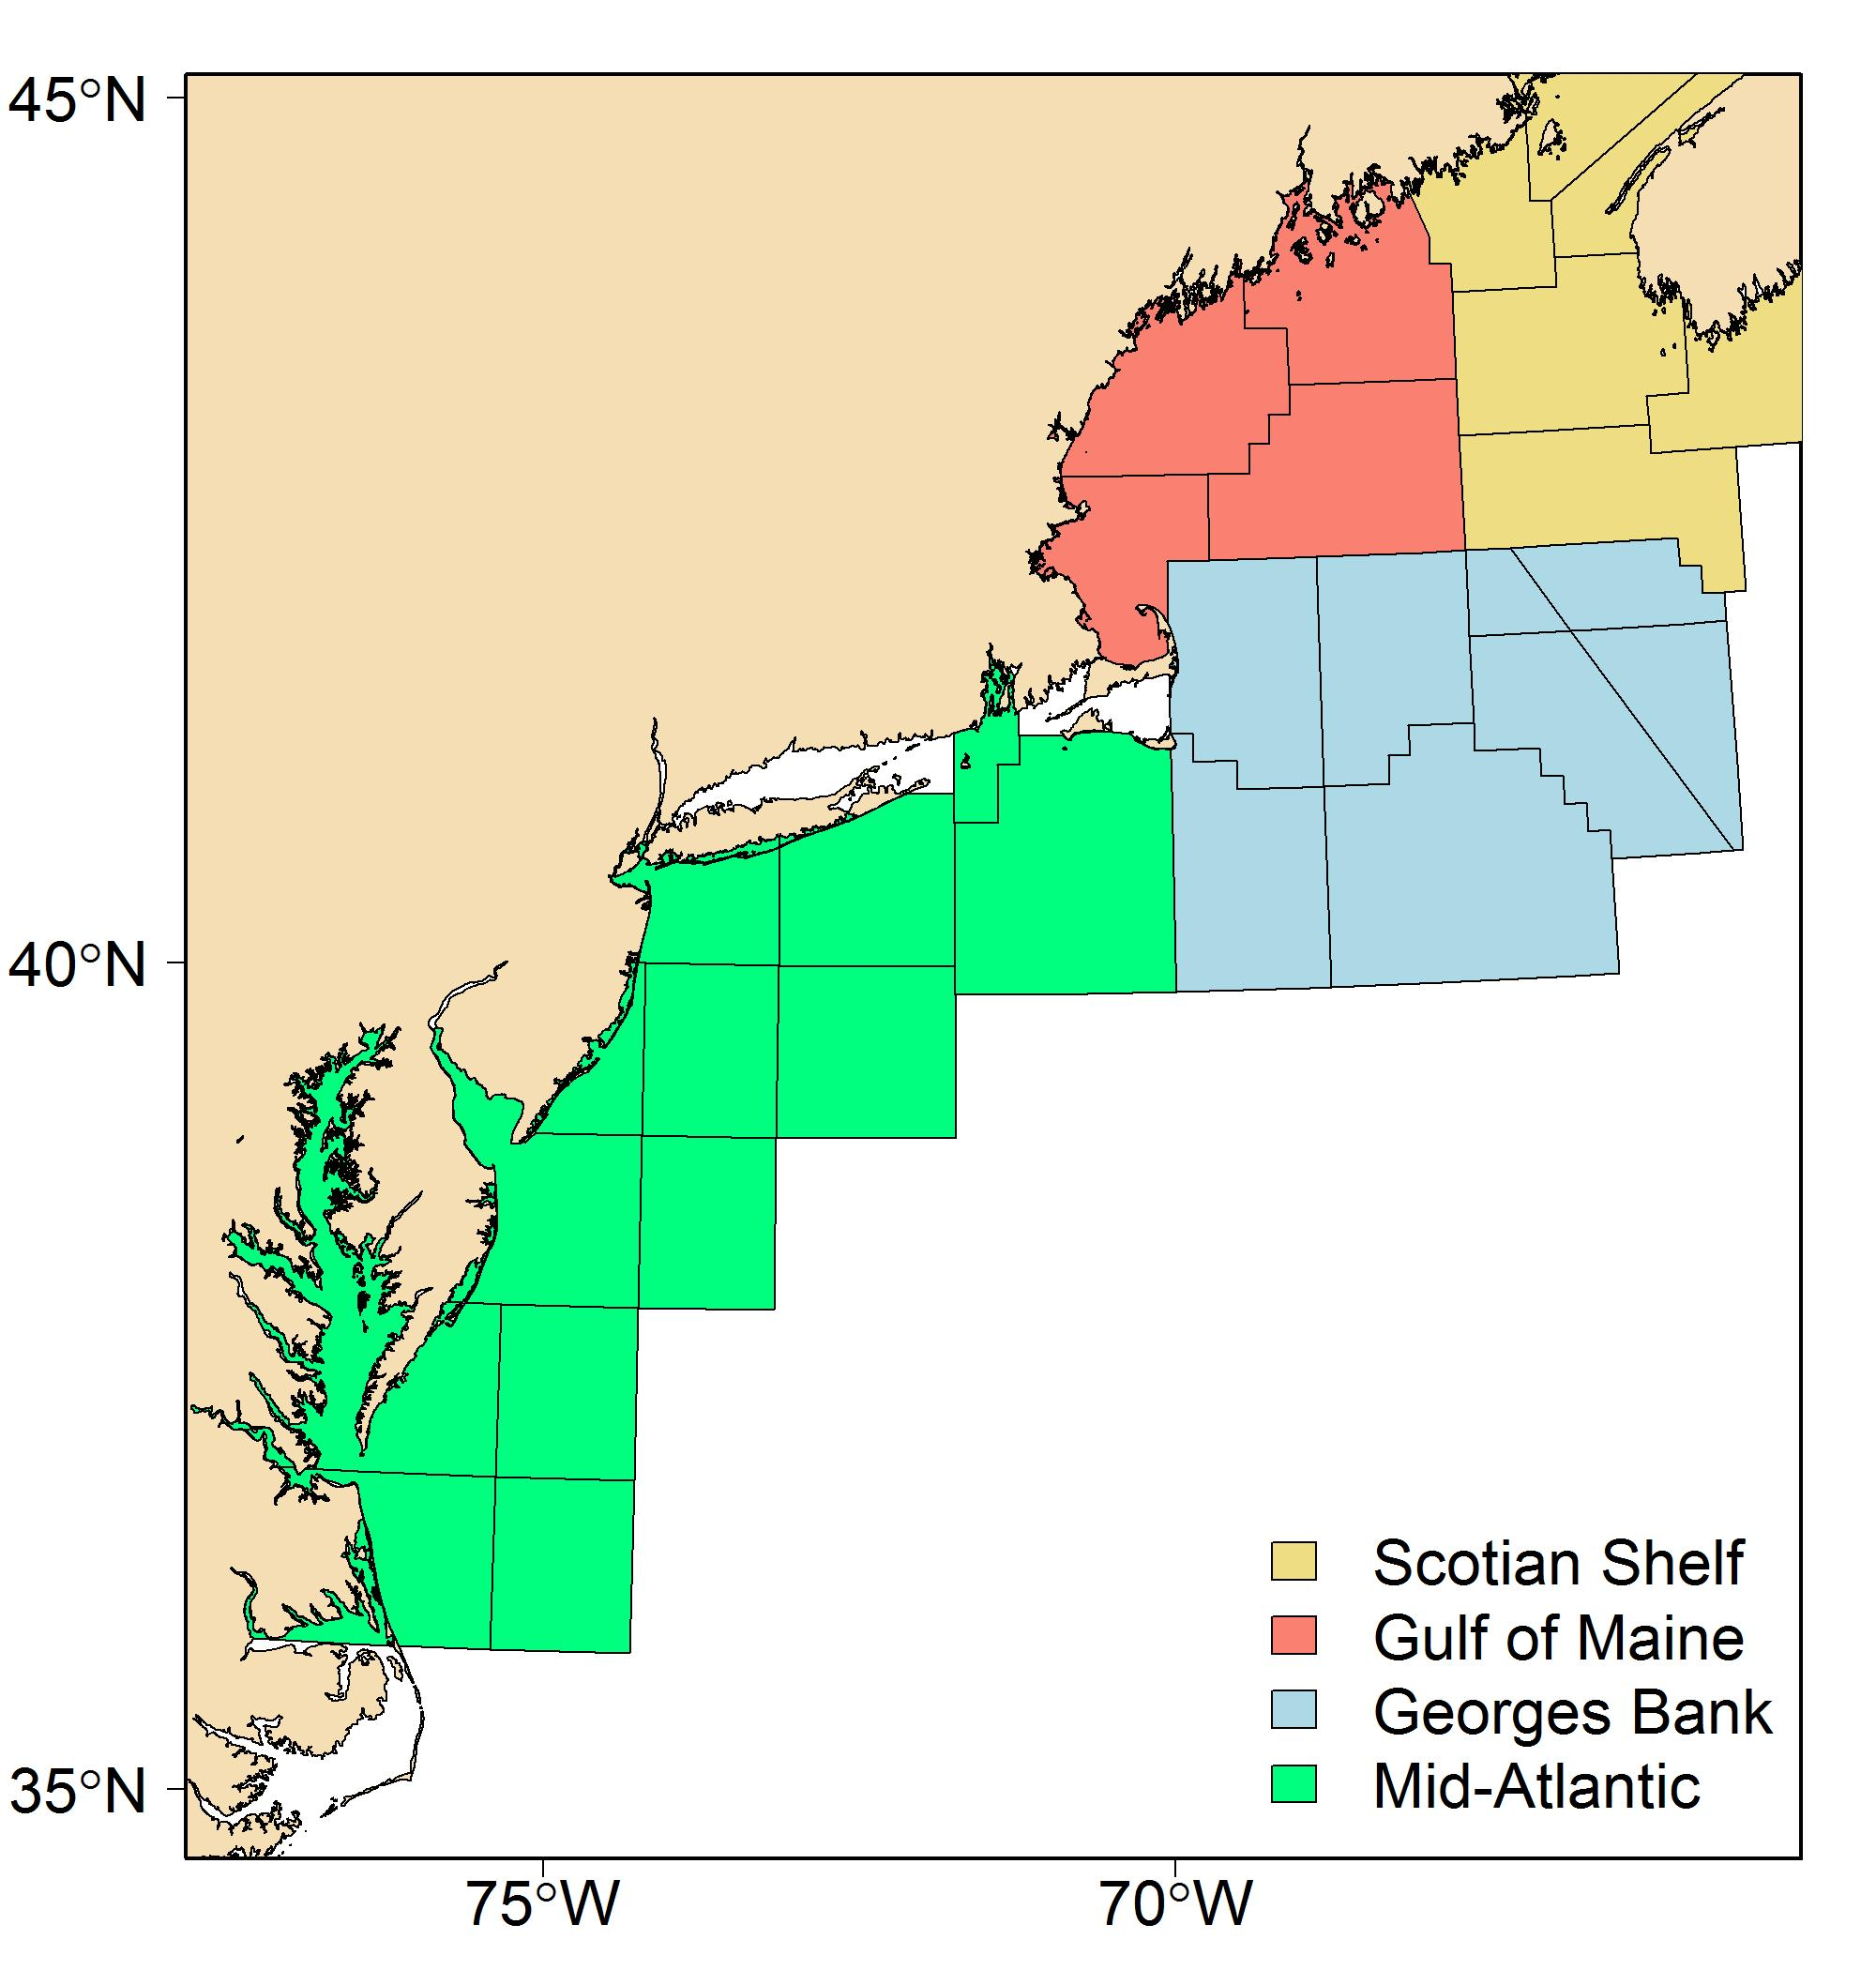
\includegraphics[width=//0.5linewidth]{/Users/seanhardison/Documents/git/tech-doc/images/Stat_Area_Map} 

}

\caption{Map of the North Atlantic Fisheries Organization (NAFO) Statistical Areas.  Colors represent the Ecological Production Unit (EPU) with which the statistical area is associated.}\label{fig:StatAreaMap}
\end{figure}

During the first section, the Comlands script pulls the temporal and
spatial information as well as vessel and gear characteristics
associated with the landings in addition to the weight, value, and
utilization code of each species in the landings record. The script
includes a toggle to use landed weights as opposed to live weights. For
all but shellfish species, live weights are used for the State of the
Ecosystem report. Due to the volume of data contained within each yearly
landings table, landings are aggregated by species, utilization code,
and area as well as by month, gear, and tonnage class. All weights are
then converted from pounds to metric tons. Landings values are also
adjusted for inflation using the Producer Price Index by Commodity for
Processed Foods and Feeds: Unprocessed and Packaged Fish. Inflation is
based on January of the terminal year of the data pull ensuring that all
values are in current dollar prices.

Several species have additional steps after the data is pulled from
CFDBS. Skates are typically landed as a species complex. In order to
segregate the catch into species, the ratio of individual skate species
in the NEFSC bottom trawl survey is used to disaggregate the landings. A
similar algorithm is used to separate silver and offshore hake which can
be mistaken for one another. Finally, Atlantic herring landings are
pulled from a separate database as the most accurate weights are housed
by the State of Maine. Comlands pulls from the State database and
replaces the less accurate numbers from the federal database.

The majority of landings data are associated with a NAFO Statistical
Area. For those that are not, Comlands attempts to assign them to an
area using similar characteristics of trips where the area is known. To
simplify this task, landings data are further aggregated into quarter
and half year, small and large vessels, and eight major gear categories
(Table @ref(tab:gears)). Landings are then proportioned to areas that
meet similar characteristics based on the proportion of landings in each
area by that temporal/vessel/gear combination. If a given attribute is
unknown, the algorithm attempts to assign it one, once again based on
matched characteristics of known trips. Statistical areas are then
assigned to their respective \protect\hyperlink{epu}{Ecological
Production Unit} (Table @ref(tab:statareas)).

\begin{table}[t]

\caption{\label{tab:gears}Gear types}
\centering
\begin{tabular}{l}
\hline
Major gear\\
\hline
Otter Trawls\\
\hline
Scallop Dredges\\
\hline
Other Dredges\\
\hline
Gillnets\\
\hline
Longlines\\
\hline
Seines\\
\hline
Pots/Traps\\
\hline
Midwater\\
\hline
Other\\
\hline
\end{tabular}
\end{table}

\begin{table}[t]

\caption{\label{tab:statareas}Statistical areas making up each EPU}
\centering
\begin{tabular}{l|l}
\hline
EPU & Stat Areas\\
\hline
Gulf of Maine & 500, 510, 512, 513, 514, 515\\
\hline
Georges Bank & 521, 522, 523, 524, 525, 526, 551, 552, 561, 562\\
\hline
Mid-Atlantic & 537, 539, 600, 612, 613, 614, 615, 616, 621, 622, 625, 626, 631, 632\\
\hline
\end{tabular}
\end{table}

The final step of Comlands is to pull the foreign landings from the
\href{https://www.nafo.int/Data/frames}{NAFO database}. US landings are
removed from this extraction so as not to be double counted. NAFO codes
and CFDBS codes differ so the script rectifies those codes to ensure
that the data is seamlessly merged into the domestic landings. Foreign
landings are flagged so that they can be removed if so desired.

\subsubsection{Data sources}\label{data-sources}

Comland is a database query of the NEFSC commercial fishery database
(CFDBS). More information about the CFDBS is available
\href{https://inport.nmfs.noaa.gov/inport/item/27401}{here}.

\subsubsection{Data extraction}\label{data-extraction}

R code used in the extraction process described above:

\begin{Shaded}
\begin{Highlighting}[]
\CommentTok{#Comland.r}
\CommentTok{#Version now controlled by git - originally part of comcatch.r}
\CommentTok{#Grab commercial landings data from US and Foreign countries (NAFO)}
\CommentTok{#Need to fix menhaden data}
\CommentTok{#SML}

\CommentTok{#Requires the following files:}
\CommentTok{# data.dir.2\textbackslash{}\textbackslash{}Comland_skates_hakes.R}
\CommentTok{# data.dir\textbackslash{}\textbackslash{}Menhaden.csv}
\CommentTok{# data.dir.3\textbackslash{}\textbackslash{}SS_NAFO_21A.csv}
\CommentTok{# data.dir.3\textbackslash{}\textbackslash{}species.txt}

\CommentTok{#User parameters}
\ControlFlowTok{if}\NormalTok{(}\KeywordTok{Sys.info}\NormalTok{()[}\StringTok{'sysname'}\NormalTok{]}\OperatorTok{==}\StringTok{"Windows"}\NormalTok{)\{}
\NormalTok{  data.dir   <-}\StringTok{ "L:}\CharTok{\textbackslash{}\textbackslash{}}\StringTok{EcoAP}\CharTok{\textbackslash{}\textbackslash{}}\StringTok{Data}\CharTok{\textbackslash{}\textbackslash{}}\StringTok{Commercial"}
\NormalTok{  data.dir.}\DecValTok{2}\NormalTok{ <-}\StringTok{ "L:}\CharTok{\textbackslash{}\textbackslash{}}\StringTok{Rworkspace}\CharTok{\textbackslash{}\textbackslash{}}\StringTok{RCom"}
\NormalTok{  data.dir.}\DecValTok{3}\NormalTok{ <-}\StringTok{ "L:}\CharTok{\textbackslash{}\textbackslash{}}\StringTok{EcoAP}\CharTok{\textbackslash{}\textbackslash{}}\StringTok{Data}\CharTok{\textbackslash{}\textbackslash{}}\StringTok{NAFO"}
\NormalTok{  out.dir    <-}\StringTok{ "L:}\CharTok{\textbackslash{}\textbackslash{}}\StringTok{EcoAP}\CharTok{\textbackslash{}\textbackslash{}}\StringTok{Data}\CharTok{\textbackslash{}\textbackslash{}}\StringTok{Commercial"}
  \KeywordTok{memory.limit}\NormalTok{(}\DecValTok{4000}\NormalTok{)}
\NormalTok{  channel <-}\StringTok{ }\KeywordTok{odbcDriverConnect}\NormalTok{()}
\NormalTok{\}}

\ControlFlowTok{if}\NormalTok{(}\KeywordTok{Sys.info}\NormalTok{()[}\StringTok{'sysname'}\NormalTok{]}\OperatorTok{==}\StringTok{"Linux"}\NormalTok{)\{}
\NormalTok{  data.dir   <-}\StringTok{ "/home/slucey/slucey/EcoAP/Data/Commercial"}
\NormalTok{  data.dir.}\DecValTok{2}\NormalTok{ <-}\StringTok{ "/home/slucey/slucey/Rworkspace/RCom"}
\NormalTok{  data.dir.}\DecValTok{3}\NormalTok{ <-}\StringTok{ "/home/slucey/slucey/EcoAP/Data/NAFO"}
\NormalTok{  out.dir    <-}\StringTok{ "/home/slucey/slucey/EcoAP/Data/Commercial"}
\NormalTok{  uid <-}\StringTok{ 'slucey'}
  \KeywordTok{cat}\NormalTok{(}\StringTok{"Oracle Password: "}\NormalTok{)}
\NormalTok{  pwd <-}\StringTok{ }\KeywordTok{scan}\NormalTok{(}\KeywordTok{stdin}\NormalTok{(), }\KeywordTok{character}\NormalTok{(), }\DataTypeTok{n =} \DecValTok{1}\NormalTok{)}
\NormalTok{\}}

\NormalTok{landed       <-}\StringTok{ 'y'} \CommentTok{#use landed weight for scallops and clams instead of live weight}
\NormalTok{foreign      <-}\StringTok{ 'y'} \CommentTok{#Mark foreign landings and keep seperate}
\NormalTok{adjust.ppi   <-}\StringTok{ 'y'} \CommentTok{#Adjust value for inflation}
\NormalTok{use.existing <-}\StringTok{ 'n'} \CommentTok{#use raw data from a previous run - saves time}
\NormalTok{sum.by       <-}\StringTok{ 'EPU'} \CommentTok{#Variable to sum landings by [EPU, stat.area]}

\CommentTok{#Final year of query}
\NormalTok{endyear <-}\StringTok{ }\DecValTok{2016}
\CommentTok{#If adjusting for inflation}
\NormalTok{refyear  <-}\StringTok{ }\DecValTok{2016}
\NormalTok{refmonth <-}\StringTok{ }\DecValTok{1}

\CommentTok{#-------------------------------------------------------------------------------}
\CommentTok{#Required packages}
\KeywordTok{library}\NormalTok{(RODBC); }\KeywordTok{library}\NormalTok{(data.table); }\KeywordTok{library}\NormalTok{(rgdal)}

\CommentTok{#-------------------------------------------------------------------------------}
\CommentTok{#User created functions }
\CommentTok{#Convert NA's to zeros}
\NormalTok{na.zero <-}\StringTok{ }\ControlFlowTok{function}\NormalTok{(x)\{}
  \ControlFlowTok{for}\NormalTok{(i }\ControlFlowTok{in} \DecValTok{1}\OperatorTok{:}\KeywordTok{length}\NormalTok{(x[}\DecValTok{1}\NormalTok{, ]))\{}
    \ControlFlowTok{if}\NormalTok{(}\KeywordTok{length}\NormalTok{(}\KeywordTok{which}\NormalTok{(}\KeywordTok{is.na}\NormalTok{(x[, i]))) }\OperatorTok{>}\StringTok{ }\DecValTok{0}\NormalTok{)\{}
\NormalTok{      x[}\KeywordTok{which}\NormalTok{(}\KeywordTok{is.na}\NormalTok{(x[, i])), i] <-}\StringTok{ }\DecValTok{0}\NormalTok{\}}
\NormalTok{    \}}
    \KeywordTok{return}\NormalTok{(x)}
\NormalTok{  \} }
  
\CommentTok{#-------------------------------------------------------------------------------}
\CommentTok{#Connect to database}
\ControlFlowTok{if}\NormalTok{(}\KeywordTok{Sys.info}\NormalTok{()[}\StringTok{'sysname'}\NormalTok{] }\OperatorTok{==}\StringTok{ "Windows"}\NormalTok{)channel <-}\StringTok{ }\KeywordTok{odbcDriverConnect}\NormalTok{()}
\ControlFlowTok{if}\NormalTok{(}\KeywordTok{Sys.info}\NormalTok{()[}\StringTok{'sysname'}\NormalTok{] }\OperatorTok{==}\StringTok{ "Linux"}\NormalTok{)  channel <-}\StringTok{ }\KeywordTok{odbcConnect}\NormalTok{(}\StringTok{'sole'}\NormalTok{, uid, pwd)}

\ControlFlowTok{if}\NormalTok{(use.existing }\OperatorTok{==}\StringTok{ 'n'}\NormalTok{)\{}
  \CommentTok{#Landings}
\NormalTok{  tables <-}\StringTok{ }\KeywordTok{c}\NormalTok{(}\KeywordTok{paste0}\NormalTok{(}\StringTok{'WOLANDS'}\NormalTok{, }\DecValTok{64}\OperatorTok{:}\DecValTok{81}\NormalTok{), }
              \KeywordTok{paste0}\NormalTok{(}\StringTok{'WODETS'}\NormalTok{,  }\DecValTok{82}\OperatorTok{:}\DecValTok{93}\NormalTok{), }
              \KeywordTok{paste0}\NormalTok{(}\StringTok{'CFDETS'}\NormalTok{,  }\DecValTok{1994}\OperatorTok{:}\NormalTok{endyear, }\StringTok{'AA'}\NormalTok{))}
  
  \CommentTok{#Generate one table}
\NormalTok{  comland <-}\StringTok{ }\KeywordTok{c}\NormalTok{()}
  \ControlFlowTok{for}\NormalTok{(i }\ControlFlowTok{in} \DecValTok{1}\OperatorTok{:}\KeywordTok{length}\NormalTok{(tables))\{}
\NormalTok{    landings.qry <-}\StringTok{ }\KeywordTok{paste}\NormalTok{(}\StringTok{"select year, month, negear, toncl1, nespp3, nespp4, area, }
\StringTok{                           spplivlb, spplndlb, sppvalue, utilcd}
\StringTok{                           from"}\NormalTok{, tables[i])}
    
\NormalTok{    comland.yr <-}\StringTok{ }\KeywordTok{as.data.table}\NormalTok{(}\KeywordTok{sqlQuery}\NormalTok{(channel, landings.qry))}
    
    \KeywordTok{setkey}\NormalTok{(comland.yr,}
\NormalTok{           YEAR,}
\NormalTok{           MONTH,}
\NormalTok{           NEGEAR,}
\NormalTok{           TONCL1,}
\NormalTok{           NESPP3,}
\NormalTok{           NESPP4,}
\NormalTok{           AREA,}
\NormalTok{           UTILCD)}
  
    \ControlFlowTok{if}\NormalTok{(landed }\OperatorTok{==}\StringTok{ 'y'}\NormalTok{) comland.yr[NESPP3 }\OperatorTok\StringTok{ }\DecValTok{743}\OperatorTok{:}\DecValTok{800}\NormalTok{, SPPLIVLB }\OperatorTok{:}\ErrorTok{=}\StringTok{ }\NormalTok{SPPLNDLB]}
    
    \CommentTok{#Sum landings and value}
    \CommentTok{#landings}
\NormalTok{    comland.yr[, V1 }\OperatorTok{:}\ErrorTok{=}\StringTok{ }\KeywordTok{sum}\NormalTok{(SPPLIVLB), by =}\StringTok{ }\KeywordTok{key}\NormalTok{(comland.yr)]}
    \CommentTok{#value}
    \CommentTok{#Fix null values}
\NormalTok{    comland.yr[}\KeywordTok{is.na}\NormalTok{(SPPVALUE), SPPVALUE }\OperatorTok{:}\ErrorTok{=}\StringTok{ }\DecValTok{0}\NormalTok{]}
\NormalTok{    comland.yr[, V2 }\OperatorTok{:}\ErrorTok{=}\StringTok{ }\KeywordTok{sum}\NormalTok{(SPPVALUE), by =}\StringTok{ }\KeywordTok{key}\NormalTok{(comland.yr)]}
    
    \CommentTok{#Remove extra rows/columns}
\NormalTok{    comland.yr <-}\StringTok{ }\KeywordTok{unique}\NormalTok{(comland.yr, }\DataTypeTok{by =} \KeywordTok{key}\NormalTok{(comland.yr))}
\NormalTok{    comland.yr[, }\KeywordTok{c}\NormalTok{(}\StringTok{'SPPLIVLB'}\NormalTok{, }\StringTok{'SPPLNDLB'}\NormalTok{, }\StringTok{'SPPVALUE'}\NormalTok{) }\OperatorTok{:}\ErrorTok{=}\StringTok{ }\OtherTok{NULL}\NormalTok{]}
    
    \CommentTok{#Rename summed columns}
    \KeywordTok{setnames}\NormalTok{(comland.yr, }\KeywordTok{c}\NormalTok{(}\StringTok{'V1'}\NormalTok{, }\StringTok{'V2'}\NormalTok{), }\KeywordTok{c}\NormalTok{(}\StringTok{'SPPLIVLB'}\NormalTok{, }\StringTok{'SPPVALUE'}\NormalTok{))}
    
\NormalTok{    comland <-}\StringTok{ }\KeywordTok{rbindlist}\NormalTok{(}\KeywordTok{list}\NormalTok{(comland, comland.yr))}
\NormalTok{  \}}
  
  \ControlFlowTok{if}\NormalTok{(landed }\OperatorTok{==}\StringTok{ 'n'}\NormalTok{) }\KeywordTok{save}\NormalTok{(comland, }\DataTypeTok{file =} \KeywordTok{file.path}\NormalTok{(out.dir, }\StringTok{"comland_raw_US.RData"}\NormalTok{))}
  \CommentTok{#Last run 8/31/16}
  \ControlFlowTok{if}\NormalTok{(landed }\OperatorTok{==}\StringTok{ 'y'}\NormalTok{) }\KeywordTok{save}\NormalTok{(comland, }\DataTypeTok{file =} \KeywordTok{file.path}\NormalTok{(out.dir, }\StringTok{"comland_raw_US_meatwt.RData"}\NormalTok{))}
  \CommentTok{#Last run 1/25/18 }
\NormalTok{\}}
\ControlFlowTok{if}\NormalTok{(use.existing }\OperatorTok{==}\StringTok{ 'y'}\NormalTok{)\{}
  \ControlFlowTok{if}\NormalTok{(landed }\OperatorTok{==}\StringTok{ 'n'}\NormalTok{) }\KeywordTok{load}\NormalTok{(}\DataTypeTok{file =} \KeywordTok{file.path}\NormalTok{(out.dir, }\StringTok{"comland_raw_US.RData"}\NormalTok{))}
  \ControlFlowTok{if}\NormalTok{(landed }\OperatorTok{==}\StringTok{ 'y'}\NormalTok{) }\KeywordTok{load}\NormalTok{(}\DataTypeTok{file =} \KeywordTok{file.path}\NormalTok{(out.dir, }\StringTok{"comland_raw_US_meatwt.RData"}\NormalTok{))  }
\NormalTok{\}}

\CommentTok{#-------------------------------------------------------------------------------}
\CommentTok{#Convert from lbs to metric tons}
\NormalTok{comland[, SPPLIVMT }\OperatorTok{:}\ErrorTok{=}\StringTok{ }\NormalTok{SPPLIVLB }\OperatorTok{*}\StringTok{ }\FloatTok{0.00045359237}\NormalTok{]}
\NormalTok{comland[, SPPLIVLB }\OperatorTok{:}\ErrorTok{=}\StringTok{ }\OtherTok{NULL}\NormalTok{]}

\CommentTok{#fix years}
\NormalTok{comland[YEAR }\OperatorTok{<}\StringTok{ }\DecValTok{100}\NormalTok{, YEAR }\OperatorTok{:}\ErrorTok{=}\StringTok{ }\NormalTok{YEAR }\OperatorTok{+}\StringTok{ }\NormalTok{1900L]}

\ControlFlowTok{if}\NormalTok{(adjust.ppi }\OperatorTok{==}\StringTok{ 'y'}\NormalTok{)\{}
    \CommentTok{#Adjust SPPVALUE for inflation}
\NormalTok{    temp <-}\StringTok{ }\KeywordTok{tempfile}\NormalTok{()}
    \KeywordTok{download.file}\NormalTok{(}\StringTok{"http://download.bls.gov/pub/time.series/wp/wp.data.3.ProcessedFoods"}\NormalTok{, temp)}
\NormalTok{    inflate <-}\StringTok{ }\KeywordTok{as.data.table}\NormalTok{(}\KeywordTok{read.delim}\NormalTok{(temp))}
    \KeywordTok{unlink}\NormalTok{(temp)}
    
\NormalTok{    inflate[, series_id }\OperatorTok{:}\ErrorTok{=}\StringTok{ }\KeywordTok{gsub}\NormalTok{(}\StringTok{" "}\NormalTok{, }\StringTok{""}\NormalTok{, inflate[, series_id])]}
\NormalTok{    deflate <-}\StringTok{ }\NormalTok{inflate[series_id }\OperatorTok{==}\StringTok{ "WPU0223"}\NormalTok{, ]}
\NormalTok{    deflate[, MONTH }\OperatorTok{:}\ErrorTok{=}\StringTok{ }\KeywordTok{as.numeric}\NormalTok{(}\KeywordTok{substr}\NormalTok{(period, }\DecValTok{2}\NormalTok{, }\DecValTok{3}\NormalTok{))]}
    \KeywordTok{setnames}\NormalTok{(deflate, }\KeywordTok{c}\NormalTok{(}\StringTok{'year'}\NormalTok{, }\StringTok{'value'}\NormalTok{), }\KeywordTok{c}\NormalTok{(}\StringTok{'YEAR'}\NormalTok{, }\StringTok{'PPI'}\NormalTok{))}
\NormalTok{    deflate <-}\StringTok{ }\NormalTok{deflate[, }\KeywordTok{list}\NormalTok{(YEAR, MONTH, PPI)]}
    
    \CommentTok{#Set yearly deflator to 0 instead of 13 to match unknown month designation}
\NormalTok{    deflate[MONTH }\OperatorTok{==}\StringTok{ }\DecValTok{13}\NormalTok{, MONTH }\OperatorTok{:}\ErrorTok{=}\StringTok{ }\DecValTok{0}\NormalTok{]}
\NormalTok{    deflate.base <-}\StringTok{ }\NormalTok{deflate[YEAR }\OperatorTok{==}\StringTok{ }\NormalTok{refyear }\OperatorTok{&}\StringTok{ }\NormalTok{MONTH }\OperatorTok{==}\StringTok{ }\NormalTok{refmonth, PPI]}
    
\NormalTok{    comland <-}\StringTok{ }\KeywordTok{merge}\NormalTok{(comland, deflate, }\DataTypeTok{by =} \KeywordTok{c}\NormalTok{(}\StringTok{'YEAR'}\NormalTok{, }\StringTok{'MONTH'}\NormalTok{), }\DataTypeTok{all.x =}\NormalTok{ T)}
\NormalTok{    comland[, SPPVALUE }\OperatorTok{:}\ErrorTok{=}\StringTok{ }\KeywordTok{round}\NormalTok{((SPPVALUE }\OperatorTok{*}\StringTok{ }\NormalTok{deflate.base) }\OperatorTok{/}\StringTok{ }\NormalTok{PPI)]}
    
    \CommentTok{#Remove extra column}
\NormalTok{    comland[, PPI }\OperatorTok{:}\ErrorTok{=}\StringTok{ }\OtherTok{NULL}\NormalTok{]}
\NormalTok{\}}
\CommentTok{#Remove market categories of parts}
\NormalTok{comland <-}\StringTok{ }\NormalTok{comland[}\OperatorTok{!}\NormalTok{NESPP4 }\OperatorTok\StringTok{ }\KeywordTok{c}\NormalTok{(}\DecValTok{119}\NormalTok{, }\DecValTok{123}\NormalTok{, }\DecValTok{125}\NormalTok{, }\DecValTok{127}\NormalTok{, }\DecValTok{812}\NormalTok{, }\DecValTok{819}\NormalTok{, }\DecValTok{828}\NormalTok{, }\DecValTok{829}\NormalTok{, }\DecValTok{1731}\NormalTok{, }\DecValTok{2351}\NormalTok{,}
                                  \DecValTok{2690}\NormalTok{, }\DecValTok{2699}\NormalTok{, }\DecValTok{3472}\NormalTok{, }\KeywordTok{as.numeric}\NormalTok{(}\KeywordTok{paste}\NormalTok{(}\DecValTok{348}\OperatorTok{:}\DecValTok{359}\NormalTok{, }\DecValTok{8}\NormalTok{, }\DataTypeTok{sep =} \StringTok{''}\NormalTok{)), }
                                  \DecValTok{3868}\NormalTok{, }\KeywordTok{as.numeric}\NormalTok{(}\KeywordTok{paste}\NormalTok{(}\DecValTok{469}\OperatorTok{:}\DecValTok{471}\NormalTok{, }\DecValTok{4}\NormalTok{, }\DataTypeTok{sep =} \StringTok{''}\NormalTok{)), }
                                  \KeywordTok{as.numeric}\NormalTok{(}\KeywordTok{paste}\NormalTok{(}\DecValTok{480}\OperatorTok{:}\DecValTok{499}\NormalTok{, }\DecValTok{8}\NormalTok{, }\DataTypeTok{sep =}\StringTok{''}\NormalTok{)), }\DecValTok{5018}\NormalTok{, }\DecValTok{5039}\NormalTok{, }
                                  \DecValTok{5261}\NormalTok{, }\DecValTok{5265}\NormalTok{), ]}

\CommentTok{#Generate NESPP3 and MKTCAT in comland data}
\NormalTok{comland[NESPP4 }\OperatorTok{<}\StringTok{ }\DecValTok{100}\NormalTok{,                MKTCAT }\OperatorTok{:}\ErrorTok{=}\StringTok{ }\KeywordTok{as.numeric}\NormalTok{(}\KeywordTok{substring}\NormalTok{(NESPP4, }\DecValTok{2}\NormalTok{, }\DecValTok{2}\NormalTok{))]}
\NormalTok{comland[NESPP4 }\OperatorTok{>}\StringTok{ }\DecValTok{99} \OperatorTok{&}\StringTok{ }\NormalTok{NESPP4 }\OperatorTok{<}\StringTok{ }\DecValTok{1000}\NormalTok{, MKTCAT }\OperatorTok{:}\ErrorTok{=}\StringTok{ }\KeywordTok{as.numeric}\NormalTok{(}\KeywordTok{substring}\NormalTok{(NESPP4, }\DecValTok{3}\NormalTok{, }\DecValTok{3}\NormalTok{))]}
\NormalTok{comland[NESPP4 }\OperatorTok{>}\StringTok{ }\DecValTok{999}\NormalTok{,                MKTCAT }\OperatorTok{:}\ErrorTok{=}\StringTok{ }\KeywordTok{as.numeric}\NormalTok{(}\KeywordTok{substring}\NormalTok{(NESPP4, }\DecValTok{4}\NormalTok{, }\DecValTok{4}\NormalTok{))]}

\CommentTok{#drop NESPP4}
\NormalTok{comland[, NESPP4 }\OperatorTok{:}\ErrorTok{=}\StringTok{ }\OtherTok{NULL}\NormalTok{]}

\CommentTok{#Deal with Hakes and Skates------------------------------------------------------------------}
\KeywordTok{source}\NormalTok{(}\KeywordTok{file.path}\NormalTok{(data.dir.}\DecValTok{2}\NormalTok{, }\StringTok{'Comland_skates_hakes.R'}\NormalTok{))}

\CommentTok{#get little skates and winter skates from skates(ns) - use survey in half years}
\CommentTok{#Generate Half year variable in comland}
\NormalTok{comland.skates <-}\StringTok{ }\NormalTok{comland[NESPP3 }\OperatorTok{==}\StringTok{ }\DecValTok{365}\NormalTok{, ]}
\NormalTok{comland.skates[MONTH }\OperatorTok\StringTok{ }\DecValTok{1}\OperatorTok{:}\DecValTok{6}\NormalTok{,  Half }\OperatorTok{:}\ErrorTok{=}\StringTok{ }\DecValTok{1}\NormalTok{]}
\NormalTok{comland.skates[MONTH }\OperatorTok\StringTok{ }\DecValTok{7}\OperatorTok{:}\DecValTok{12}\NormalTok{, Half }\OperatorTok{:}\ErrorTok{=}\StringTok{ }\DecValTok{2}\NormalTok{]}

\KeywordTok{setkey}\NormalTok{(skate.hake.us,}
\NormalTok{       YEAR,}
\NormalTok{       Half,}
\NormalTok{       AREA)}

\NormalTok{comland.skates <-}\StringTok{ }\KeywordTok{merge}\NormalTok{(comland.skates, skate.hake.us, }\DataTypeTok{by =} \KeywordTok{key}\NormalTok{(skate.hake.us), }\DataTypeTok{all.x =}\NormalTok{ T)}

\NormalTok{comland.skates[, little       }\OperatorTok{:}\ErrorTok{=}\StringTok{ }\NormalTok{little.per }\OperatorTok{*}\StringTok{ }\NormalTok{SPPLIVMT]}
\NormalTok{comland.skates[, little.value }\OperatorTok{:}\ErrorTok{=}\StringTok{ }\KeywordTok{round}\NormalTok{(little.per }\OperatorTok{*}\StringTok{ }\NormalTok{SPPVALUE)]}
\NormalTok{comland.skates[}\KeywordTok{is.na}\NormalTok{(little),       little       }\OperatorTok{:}\ErrorTok{=}\StringTok{ }\DecValTok{0}\NormalTok{]}
\NormalTok{comland.skates[}\KeywordTok{is.na}\NormalTok{(little.value), little.value }\OperatorTok{:}\ErrorTok{=}\StringTok{ }\DecValTok{0}\NormalTok{]}

\NormalTok{comland.skates[, winter       }\OperatorTok{:}\ErrorTok{=}\StringTok{ }\NormalTok{winter.per }\OperatorTok{*}\StringTok{ }\NormalTok{SPPLIVMT]}
\NormalTok{comland.skates[, winter.value }\OperatorTok{:}\ErrorTok{=}\StringTok{ }\KeywordTok{round}\NormalTok{(winter.per }\OperatorTok{*}\StringTok{ }\NormalTok{SPPVALUE)]}
\NormalTok{comland.skates[}\KeywordTok{is.na}\NormalTok{(winter),       winter       }\OperatorTok{:}\ErrorTok{=}\StringTok{ }\DecValTok{0}\NormalTok{]}
\NormalTok{comland.skates[}\KeywordTok{is.na}\NormalTok{(winter.value), winter.value }\OperatorTok{:}\ErrorTok{=}\StringTok{ }\DecValTok{0}\NormalTok{]}

\NormalTok{comland.skates[, other.skate       }\OperatorTok{:}\ErrorTok{=}\StringTok{ }\NormalTok{SPPLIVMT }\OperatorTok{-}\StringTok{ }\NormalTok{(little       }\OperatorTok{+}\StringTok{ }\NormalTok{winter)]}
\NormalTok{comland.skates[, other.skate.value }\OperatorTok{:}\ErrorTok{=}\StringTok{ }\NormalTok{SPPVALUE }\OperatorTok{-}\StringTok{ }\NormalTok{(little.value }\OperatorTok{+}\StringTok{ }\NormalTok{winter.value)]}

\CommentTok{#Little (366), winter (367), skates(ns) (365)}
\CommentTok{#put skates in comland format to merge back}
\NormalTok{little <-}\StringTok{ }\NormalTok{comland.skates[, }\KeywordTok{list}\NormalTok{(YEAR, Half, AREA, MONTH, NEGEAR,}
\NormalTok{                                TONCL1, NESPP3, UTILCD, MKTCAT, little, }
\NormalTok{                                little.value)]}
\NormalTok{little[, NESPP3 }\OperatorTok{:}\ErrorTok{=}\StringTok{ }\DecValTok{366}\NormalTok{]}
\KeywordTok{setnames}\NormalTok{(little, }\KeywordTok{c}\NormalTok{(}\StringTok{'little'}\NormalTok{, }\StringTok{'little.value'}\NormalTok{), }\KeywordTok{c}\NormalTok{(}\StringTok{'SPPLIVMT'}\NormalTok{, }\StringTok{'SPPVALUE'}\NormalTok{))}
\NormalTok{little <-}\StringTok{ }\NormalTok{little[SPPLIVMT }\OperatorTok{>}\StringTok{ }\DecValTok{0}\NormalTok{, ]}

\NormalTok{winter <-}\StringTok{ }\NormalTok{comland.skates[, }\KeywordTok{list}\NormalTok{(YEAR, Half, AREA, MONTH, NEGEAR,}
\NormalTok{                                TONCL1, NESPP3, UTILCD, MKTCAT, winter, }
\NormalTok{                                winter.value)]}
\NormalTok{winter[, NESPP3 }\OperatorTok{:}\ErrorTok{=}\StringTok{ }\DecValTok{367}\NormalTok{]}
\KeywordTok{setnames}\NormalTok{(winter, }\KeywordTok{c}\NormalTok{(}\StringTok{'winter'}\NormalTok{, }\StringTok{'winter.value'}\NormalTok{), }\KeywordTok{c}\NormalTok{(}\StringTok{'SPPLIVMT'}\NormalTok{, }\StringTok{'SPPVALUE'}\NormalTok{))}
\NormalTok{winter <-}\StringTok{ }\NormalTok{winter[SPPLIVMT }\OperatorTok{>}\StringTok{ }\DecValTok{0}\NormalTok{, ]}

\NormalTok{other <-}\StringTok{ }\NormalTok{comland.skates[, }\KeywordTok{list}\NormalTok{(YEAR, Half, AREA, MONTH, NEGEAR,}
\NormalTok{                               TONCL1, NESPP3, UTILCD, MKTCAT, other.skate, }
\NormalTok{                               other.skate.value)]}
\NormalTok{other[, NESPP3 }\OperatorTok{:}\ErrorTok{=}\StringTok{ }\DecValTok{365}\NormalTok{]}
\KeywordTok{setnames}\NormalTok{(other, }\KeywordTok{c}\NormalTok{(}\StringTok{'other.skate'}\NormalTok{, }\StringTok{'other.skate.value'}\NormalTok{), }\KeywordTok{c}\NormalTok{(}\StringTok{'SPPLIVMT'}\NormalTok{, }\StringTok{'SPPVALUE'}\NormalTok{))}
\NormalTok{other <-}\StringTok{ }\NormalTok{other[SPPLIVMT }\OperatorTok{>}\StringTok{ }\DecValTok{0}\NormalTok{, ]}

\CommentTok{#merge all three and reformat for comland}
\NormalTok{skates.add.back <-}\StringTok{ }\KeywordTok{rbindlist}\NormalTok{(}\KeywordTok{list}\NormalTok{(little, winter, other))}

\NormalTok{skates.add.back[, Half }\OperatorTok{:}\ErrorTok{=}\StringTok{ }\OtherTok{NULL}\NormalTok{]}
\KeywordTok{setcolorder}\NormalTok{(skates.add.back, }\KeywordTok{names}\NormalTok{(comland))}

\NormalTok{comland <-}\StringTok{ }\KeywordTok{rbindlist}\NormalTok{(}\KeywordTok{list}\NormalTok{(comland[NESPP3 }\OperatorTok{!=}\StringTok{ }\DecValTok{365}\NormalTok{, ], skates.add.back))  }

\CommentTok{#get silver hake from mixed hakes - use survey in half years}
\CommentTok{#Generate Half year variable in comland}
\NormalTok{comland.hakes <-}\StringTok{ }\NormalTok{comland[NESPP3 }\OperatorTok{==}\StringTok{ }\DecValTok{507}\NormalTok{, ]}
\NormalTok{comland.hakes[MONTH }\OperatorTok\StringTok{ }\DecValTok{1}\OperatorTok{:}\DecValTok{6}\NormalTok{,  Half }\OperatorTok{:}\ErrorTok{=}\StringTok{ }\DecValTok{1}\NormalTok{]}
\NormalTok{comland.hakes[MONTH }\OperatorTok\StringTok{ }\DecValTok{7}\OperatorTok{:}\DecValTok{12}\NormalTok{, Half }\OperatorTok{:}\ErrorTok{=}\StringTok{ }\DecValTok{2}\NormalTok{]}

\NormalTok{comland.hakes <-}\StringTok{ }\KeywordTok{merge}\NormalTok{(comland.hakes, skate.hake.us, }\DataTypeTok{by =} \KeywordTok{key}\NormalTok{(skate.hake.us), }\DataTypeTok{all.x =}\NormalTok{ T)}

\NormalTok{comland.hakes[, silver       }\OperatorTok{:}\ErrorTok{=}\StringTok{ }\NormalTok{silver.per }\OperatorTok{*}\StringTok{ }\NormalTok{SPPLIVMT]}
\NormalTok{comland.hakes[, silver.value }\OperatorTok{:}\ErrorTok{=}\StringTok{ }\KeywordTok{round}\NormalTok{(silver.per }\OperatorTok{*}\StringTok{ }\NormalTok{SPPVALUE)]}
\NormalTok{comland.hakes[}\KeywordTok{is.na}\NormalTok{(silver),       silver       }\OperatorTok{:}\ErrorTok{=}\StringTok{ }\DecValTok{0}\NormalTok{]}
\NormalTok{comland.hakes[}\KeywordTok{is.na}\NormalTok{(silver.value), silver.value }\OperatorTok{:}\ErrorTok{=}\StringTok{ }\DecValTok{0}\NormalTok{]}

\NormalTok{comland.hakes[, off.hake       }\OperatorTok{:}\ErrorTok{=}\StringTok{ }\NormalTok{SPPLIVMT }\OperatorTok{-}\StringTok{ }\NormalTok{silver]}
\NormalTok{comland.hakes[, off.hake.value }\OperatorTok{:}\ErrorTok{=}\StringTok{ }\NormalTok{SPPVALUE }\OperatorTok{-}\StringTok{ }\NormalTok{silver.value]}

\CommentTok{#Silver hake (509), mix hakes (507)}
\CommentTok{#put hakes in comland format to merge back}
\NormalTok{silver <-}\StringTok{ }\NormalTok{comland.hakes[, }\KeywordTok{list}\NormalTok{(YEAR, Half, AREA, MONTH, NEGEAR,}
\NormalTok{                               TONCL1, NESPP3, UTILCD, MKTCAT, silver, }
\NormalTok{                               silver.value)]}
\NormalTok{silver[, NESPP3 }\OperatorTok{:}\ErrorTok{=}\StringTok{ }\DecValTok{509}\NormalTok{]}
\KeywordTok{setnames}\NormalTok{(silver, }\KeywordTok{c}\NormalTok{(}\StringTok{'silver'}\NormalTok{, }\StringTok{'silver.value'}\NormalTok{), }\KeywordTok{c}\NormalTok{(}\StringTok{'SPPLIVMT'}\NormalTok{, }\StringTok{'SPPVALUE'}\NormalTok{))}
\NormalTok{silver <-}\StringTok{ }\NormalTok{silver[SPPLIVMT }\OperatorTok{>}\StringTok{ }\DecValTok{0}\NormalTok{, ]}

\NormalTok{offshore <-}\StringTok{ }\NormalTok{comland.hakes[, }\KeywordTok{list}\NormalTok{(YEAR, Half, AREA, MONTH, NEGEAR,}
\NormalTok{                                 TONCL1, NESPP3, UTILCD, MKTCAT, off.hake, }
\NormalTok{                                 off.hake.value)]}
\NormalTok{offshore[, NESPP3 }\OperatorTok{:}\ErrorTok{=}\StringTok{ }\DecValTok{507}\NormalTok{]}
\KeywordTok{setnames}\NormalTok{(offshore, }\KeywordTok{c}\NormalTok{(}\StringTok{'off.hake'}\NormalTok{, }\StringTok{'off.hake.value'}\NormalTok{), }\KeywordTok{c}\NormalTok{(}\StringTok{'SPPLIVMT'}\NormalTok{, }\StringTok{'SPPVALUE'}\NormalTok{))}
\NormalTok{offshore <-}\StringTok{ }\NormalTok{offshore[SPPLIVMT }\OperatorTok{>}\StringTok{ }\DecValTok{0}\NormalTok{, ]}

\CommentTok{#merge both and reformat for comland}
\NormalTok{hakes.add.back <-}\StringTok{ }\KeywordTok{rbindlist}\NormalTok{(}\KeywordTok{list}\NormalTok{(silver, offshore))}

\NormalTok{hakes.add.back[, Half }\OperatorTok{:}\ErrorTok{=}\StringTok{ }\OtherTok{NULL}\NormalTok{]}
\KeywordTok{setcolorder}\NormalTok{(hakes.add.back, }\KeywordTok{names}\NormalTok{(comland))}

\NormalTok{comland <-}\StringTok{ }\KeywordTok{rbindlist}\NormalTok{(}\KeywordTok{list}\NormalTok{(comland[NESPP3 }\OperatorTok{!=}\StringTok{ }\DecValTok{507}\NormalTok{, ], hakes.add.back))}


\CommentTok{#Herring---------------------------------------------------------------------------------}
\CommentTok{#Herring data is housed by the state of Maine.}
\NormalTok{herr.qry <-}\StringTok{ "select year, month, stock_area, negear, gearname, keptmt, discmt}
\StringTok{             from maine_herring_catch"}

\NormalTok{herr.catch <-}\StringTok{ }\KeywordTok{as.data.table}\NormalTok{(}\KeywordTok{sqlQuery}\NormalTok{(channel, herr.qry))}
\KeywordTok{setkey}\NormalTok{(herr.catch, YEAR, MONTH, STOCK_AREA, NEGEAR)}

\NormalTok{herring <-}\StringTok{ }\NormalTok{herr.catch[, }\KeywordTok{list}\NormalTok{(}\KeywordTok{sum}\NormalTok{(KEPTMT), }\KeywordTok{sum}\NormalTok{(DISCMT)), by =}\StringTok{ }\KeywordTok{key}\NormalTok{(herr.catch)]}
\KeywordTok{setnames}\NormalTok{(herring, }\KeywordTok{c}\NormalTok{(}\StringTok{'STOCK_AREA'}\NormalTok{, }\StringTok{'V1'}\NormalTok{, }\StringTok{'V2'}\NormalTok{),}
                  \KeywordTok{c}\NormalTok{(}\StringTok{'AREA'}\NormalTok{, }\StringTok{'SPPLIVMT'}\NormalTok{, }\StringTok{'DISCMT'}\NormalTok{))}

\CommentTok{#Using averages from comland to fill in categories}
\NormalTok{herring[, MKTCAT }\OperatorTok{:}\ErrorTok{=}\StringTok{ }\DecValTok{5}\NormalTok{]}
\NormalTok{herring[, TONCL1 }\OperatorTok{:}\ErrorTok{=}\StringTok{ }\DecValTok{2}\NormalTok{]}
\NormalTok{herring[, UTILCD }\OperatorTok{:}\ErrorTok{=}\StringTok{ }\DecValTok{0}\NormalTok{]}

\CommentTok{#compute price/utilization from CF tables}
\NormalTok{herring.comland <-}\StringTok{ }\NormalTok{comland[NESPP3 }\OperatorTok{==}\StringTok{ }\DecValTok{168}\NormalTok{, ]}
\CommentTok{#Price from comland}
\NormalTok{herring.price <-}\StringTok{ }\NormalTok{herring.comland[, (}\KeywordTok{sum}\NormalTok{(SPPVALUE) }\OperatorTok{/}\StringTok{ }\KeywordTok{sum}\NormalTok{(SPPLIVMT)), by =}\StringTok{ }\KeywordTok{c}\NormalTok{(}\StringTok{'YEAR'}\NormalTok{, }\StringTok{'MONTH'}\NormalTok{)]}
\KeywordTok{setnames}\NormalTok{(herring.price, }\StringTok{'V1'}\NormalTok{, }\StringTok{'price'}\NormalTok{)}
\NormalTok{herring <-}\StringTok{ }\KeywordTok{merge}\NormalTok{(herring, herring.price, }\DataTypeTok{by =} \KeywordTok{c}\NormalTok{(}\StringTok{'YEAR'}\NormalTok{, }\StringTok{'MONTH'}\NormalTok{), }\DataTypeTok{all.x =}\NormalTok{ T)}
\CommentTok{#Use 1964 prices for < 1964}
\NormalTok{herring[YEAR }\OperatorTok{<}\StringTok{ }\DecValTok{1964}\NormalTok{, price }\OperatorTok{:}\ErrorTok{=}\StringTok{ }\KeywordTok{mean}\NormalTok{(herring[YEAR }\OperatorTok{==}\StringTok{ }\DecValTok{1964}\NormalTok{, price])]}
\CommentTok{#Calculate SPPVALUE from price}
\NormalTok{herring[, SPPVALUE }\OperatorTok{:}\ErrorTok{=}\StringTok{ }\KeywordTok{round}\NormalTok{(price }\OperatorTok{*}\StringTok{ }\NormalTok{SPPLIVMT)]}

\CommentTok{#Utilization from comland}
\NormalTok{herring.util <-}\StringTok{ }\NormalTok{herring.comland[, }\KeywordTok{sum}\NormalTok{(SPPLIVMT), by =}\StringTok{ }\KeywordTok{c}\NormalTok{(}\StringTok{'YEAR'}\NormalTok{, }\StringTok{'MONTH'}\NormalTok{, }\StringTok{'UTILCD'}\NormalTok{)]}
\KeywordTok{setnames}\NormalTok{(herring.util, }\StringTok{'V1'}\NormalTok{, }\StringTok{'SPPLIVMT'}\NormalTok{)}
\NormalTok{herring.util[, SPPLIVMT.ALL }\OperatorTok{:}\ErrorTok{=}\StringTok{ }\KeywordTok{sum}\NormalTok{(SPPLIVMT), by =}\StringTok{ }\KeywordTok{c}\NormalTok{(}\StringTok{'YEAR'}\NormalTok{, }\StringTok{'MONTH'}\NormalTok{)]}
\NormalTok{herring.util[, Prop }\OperatorTok{:}\ErrorTok{=}\StringTok{ }\NormalTok{SPPLIVMT}\OperatorTok{/}\NormalTok{SPPLIVMT.ALL]}
\KeywordTok{setorder}\NormalTok{(herring.util, YEAR, MONTH, Prop)}
\NormalTok{herring.util[, cum.prop }\OperatorTok{:}\ErrorTok{=}\StringTok{ }\KeywordTok{cumsum}\NormalTok{(Prop), by =}\StringTok{ }\KeywordTok{c}\NormalTok{(}\StringTok{'YEAR'}\NormalTok{, }\StringTok{'MONTH'}\NormalTok{)]}

\CommentTok{#Apply proportions to Maine data set}
\CommentTok{#Not pulled all the time - current through 2017}
\NormalTok{herring[, Total }\OperatorTok{:}\ErrorTok{=}\StringTok{ }\KeywordTok{sum}\NormalTok{(SPPLIVMT), by =}\StringTok{ }\KeywordTok{c}\NormalTok{(}\StringTok{'YEAR'}\NormalTok{, }\StringTok{'MONTH'}\NormalTok{)]}
\NormalTok{herring[, Prop }\OperatorTok{:}\ErrorTok{=}\StringTok{ }\NormalTok{SPPLIVMT }\OperatorTok{/}\StringTok{ }\NormalTok{Total]}
\KeywordTok{setorder}\NormalTok{(herring, YEAR, MONTH, Prop)}
\NormalTok{herring[, cum.prop }\OperatorTok{:}\ErrorTok{=}\StringTok{ }\KeywordTok{cumsum}\NormalTok{(Prop), by =}\StringTok{ }\KeywordTok{c}\NormalTok{(}\StringTok{'YEAR'}\NormalTok{, }\StringTok{'MONTH'}\NormalTok{)]}

\ControlFlowTok{for}\NormalTok{(iyear }\ControlFlowTok{in} \KeywordTok{unique}\NormalTok{(herring.util[, YEAR]))\{}
  \ControlFlowTok{for}\NormalTok{(imonth }\ControlFlowTok{in} \KeywordTok{unique}\NormalTok{(herring.util[YEAR }\OperatorTok{==}\StringTok{ }\NormalTok{iyear, MONTH]))\{}
\NormalTok{    cum.prop.low <-}\StringTok{ }\DecValTok{0}
    \ControlFlowTok{for}\NormalTok{(iutil }\ControlFlowTok{in}\NormalTok{ herring.util[YEAR }\OperatorTok{==}\StringTok{ }\NormalTok{iyear }\OperatorTok{&}\StringTok{ }\NormalTok{MONTH }\OperatorTok{==}\StringTok{ }\NormalTok{imonth, UTILCD])\{}
\NormalTok{      cum.prop.high <-}\StringTok{ }\NormalTok{herring.util[YEAR }\OperatorTok{==}\StringTok{ }\NormalTok{iyear }\OperatorTok{&}\StringTok{ }\NormalTok{MONTH }\OperatorTok{==}\StringTok{ }\NormalTok{imonth }\OperatorTok{&}\StringTok{ }
\StringTok{                                      }\NormalTok{UTILCD }\OperatorTok{==}\StringTok{ }\NormalTok{iutil, cum.prop]}
\NormalTok{      herring[YEAR }\OperatorTok{==}\StringTok{ }\NormalTok{iyear }\OperatorTok{&}\StringTok{ }\NormalTok{MONTH }\OperatorTok{==}\StringTok{ }\NormalTok{imonth }\OperatorTok{&}\StringTok{ }\NormalTok{cum.prop }\OperatorTok{<=}\StringTok{ }\NormalTok{cum.prop.high }\OperatorTok{&}
\StringTok{                }\NormalTok{cum.prop }\OperatorTok{>}\StringTok{ }\NormalTok{cum.prop.low, UTILCD }\OperatorTok{:}\ErrorTok{=}\StringTok{ }\NormalTok{iutil]}
\NormalTok{      cum.prop.low <-}\StringTok{ }\NormalTok{cum.prop.high}
\NormalTok{    \}}
\NormalTok{  \}}
\NormalTok{\}}

\CommentTok{#fix column headings}
\NormalTok{herring[, }\KeywordTok{c}\NormalTok{(}\StringTok{'Total'}\NormalTok{, }\StringTok{'Prop'}\NormalTok{, }\StringTok{'cum.prop'}\NormalTok{, }\StringTok{'price'}\NormalTok{, }\StringTok{'DISCMT'}\NormalTok{) }\OperatorTok{:}\ErrorTok{=}\StringTok{ }\OtherTok{NULL}\NormalTok{]}
\NormalTok{herring[, NESPP3 }\OperatorTok{:}\ErrorTok{=}\StringTok{ }\DecValTok{168}\NormalTok{]}
\KeywordTok{setcolorder}\NormalTok{(herring, }\KeywordTok{names}\NormalTok{(comland))}

\CommentTok{#remove herring from data pull and add in Maine numbers}
\NormalTok{comland <-}\StringTok{ }\KeywordTok{rbindlist}\NormalTok{(}\KeywordTok{list}\NormalTok{(comland[NESPP3 }\OperatorTok{!=}\StringTok{ }\DecValTok{168}\NormalTok{, ], herring))}

\CommentTok{#Menhaden------------------------------------------------------------------------------------}
\NormalTok{##fix menhaden records - data from Tom Miller/ Andre Bouchheister}
\CommentTok{#menhaden <- as.data.table(read.csv(paste(data.dir, "Menhaden.csv", sep = '')))}
\CommentTok{#menhaden.mab <- menhaden[, MA.Total + CB.Total, by = Year]}
\NormalTok{##file metric is 1000s of lbs - convert to mt}
\CommentTok{#menhaden.mab[, SPPLIVMT := (V1 * 1000) *  0.00045359237]}
\CommentTok{#menhaden.mab[, V1 := NULL]}
\CommentTok{#}
\CommentTok{#menhaden.gom <- menhaden[, list(Year, NE.Total)]}
\CommentTok{#menhaden.gom[, SPPLIVMT := (NE.Total * 1000) *  0.00045359237]}
\CommentTok{#menhaden.gom[, NE.Total := NULL]}

\CommentTok{#save(comland, file = paste(out.dir, "Comland_unkA.RData", sep = ''))}

\CommentTok{#Deal with unknowns-------------------------------------------------------------------------}
\NormalTok{comland[NEGEAR }\OperatorTok{==}\StringTok{ }\DecValTok{999}\NormalTok{,  NEGEAR }\OperatorTok{:}\ErrorTok{=}\StringTok{ }\DecValTok{0}\NormalTok{]}
\NormalTok{comland[}\KeywordTok{is.na}\NormalTok{(TONCL1),  TONCL1 }\OperatorTok{:}\ErrorTok{=}\StringTok{ }\DecValTok{0}\NormalTok{]}
\NormalTok{comland[}\KeywordTok{is.na}\NormalTok{(AREA),    AREA   }\OperatorTok{:}\ErrorTok{=}\StringTok{ }\KeywordTok{as.factor}\NormalTok{(}\DecValTok{0}\NormalTok{)]}
\NormalTok{comland[AREA }\OperatorTok{==}\StringTok{ }\DecValTok{999}\NormalTok{,    AREA   }\OperatorTok{:}\ErrorTok{=}\StringTok{ }\KeywordTok{as.factor}\NormalTok{(}\DecValTok{0}\NormalTok{)]}
\NormalTok{comland[}\KeywordTok{is.na}\NormalTok{(MKTCAT),  MKTCAT }\OperatorTok{:}\ErrorTok{=}\StringTok{ }\DecValTok{0}\NormalTok{]}
\NormalTok{comland[}\KeywordTok{is.na}\NormalTok{(UTILCD),  UTILCD }\OperatorTok{:}\ErrorTok{=}\StringTok{ }\DecValTok{0}\NormalTok{]}

\CommentTok{#1 - drop unknown species/landings}
\NormalTok{comland <-}\StringTok{ }\NormalTok{comland[NESPP3 }\OperatorTok{!=}\StringTok{ }\DecValTok{0} \OperatorTok{&}\StringTok{ }\NormalTok{SPPLIVMT }\OperatorTok{!=}\StringTok{ }\DecValTok{0}\NormalTok{, ]}

\CommentTok{#Sumarry tables}
\CommentTok{#missing area}
\CommentTok{#known.area <-   comland[AREA != 0, sum(SPPLIVMT), by = NESPP3]}
\CommentTok{#unknown.area <- comland[AREA == 0, sum(SPPLIVMT), by = NESPP3]}
\CommentTok{#setnames(known.area,   "V1", "AREA.MT.known")}
\CommentTok{#setnames(unknown.area, "V1", "AREA.MT.unknown")}
\CommentTok{#missing.table <- merge(known.area, unknown.area, by = 'NESPP3', all = T)}
\CommentTok{#}
\CommentTok{#missing.table[is.na(AREA.MT.known),   AREA.MT.known   := 0]}
\CommentTok{#missing.table[is.na(AREA.MT.unknown), AREA.MT.unknown := 0]}
\CommentTok{#missing.table[, AREA.Ratio := AREA.MT.unknown / AREA.MT.known]}
\CommentTok{#}
\NormalTok{##missing month}
\CommentTok{#known.month <-   comland[MONTH != 0, sum(SPPLIVMT), by = NESPP3]}
\CommentTok{#unknown.month <- comland[MONTH == 0, sum(SPPLIVMT), by = NESPP3]}
\CommentTok{#setnames(known.month,   "V1", "MONTH.MT.known")}
\CommentTok{#setnames(unknown.month, "V1", "MONTH.MT.unknown")}
\CommentTok{#missing.table <- merge(missing.table, known.month,   by = 'NESPP3', all = T)}
\CommentTok{#missing.table <- merge(missing.table, unknown.month, by = 'NESPP3', all = T)}
\CommentTok{#}
\CommentTok{#missing.table[is.na(MONTH.MT.known),   MONTH.MT.known   := 0]}
\CommentTok{#missing.table[is.na(MONTH.MT.unknown), MONTH.MT.unknown := 0]}
\CommentTok{#missing.table[, MONTH.Ratio := MONTH.MT.unknown / MONTH.MT.known]}
\CommentTok{#}
\NormalTok{##missing gear}
\CommentTok{#known.gear <-   comland[NEGEAR != 0, sum(SPPLIVMT), by = NESPP3]}
\CommentTok{#unknown.gear <- comland[NEGEAR == 0, sum(SPPLIVMT), by = NESPP3]}
\CommentTok{#setnames(known.gear,   "V1", "GEAR.MT.known")}
\CommentTok{#setnames(unknown.gear, "V1", "GEAR.MT.unknown")}
\CommentTok{#missing.table <- merge(missing.table, known.gear,   by = 'NESPP3', all = T)}
\CommentTok{#missing.table <- merge(missing.table, unknown.gear, by = 'NESPP3', all = T)}
\CommentTok{#}
\CommentTok{#missing.table[is.na(GEAR.MT.known),   GEAR.MT.known   := 0]}
\CommentTok{#missing.table[is.na(GEAR.MT.unknown), GEAR.MT.unknown := 0]}
\CommentTok{#missing.table[, GEAR.Ratio := GEAR.MT.unknown / GEAR.MT.known]}
\CommentTok{#}
\NormalTok{##missing tonnage class}
\CommentTok{#known.tc <-   comland[TONCL1 != 0, sum(SPPLIVMT), by = NESPP3]}
\CommentTok{#unknown.tc <- comland[TONCL1 == 0, sum(SPPLIVMT), by = NESPP3]}
\CommentTok{#setnames(known.tc,   "V1", "TC.MT.known")}
\CommentTok{#setnames(unknown.tc, "V1", "TC.MT.unknown")}
\CommentTok{#missing.table <- merge(missing.table, known.tc,   by = 'NESPP3', all = T)}
\CommentTok{#missing.table <- merge(missing.table, unknown.tc, by = 'NESPP3', all = T)}
\CommentTok{#}
\CommentTok{#missing.table[is.na(TC.MT.known),   TC.MT.known   := 0]}
\CommentTok{#missing.table[is.na(TC.MT.unknown), TC.MT.unknown := 0]}
\CommentTok{#missing.table[, TC.Ratio := TC.MT.unknown / TC.MT.known]}
\CommentTok{#}
\CommentTok{#write.csv(missing.table, paste(out.dir, "\textbackslash{}\textbackslash{}Missing_table.csv", sep = ''), row.names = F)}
\CommentTok{#}

\CommentTok{#2 - aggregate by quarter year, half year, major gear, and small/large TC}
\NormalTok{comland[MONTH }\OperatorTok\StringTok{ }\DecValTok{1}\OperatorTok{:}\DecValTok{3}\NormalTok{,   QY }\OperatorTok{:}\ErrorTok{=}\StringTok{ }\DecValTok{1}\NormalTok{]}
\NormalTok{comland[MONTH }\OperatorTok\StringTok{ }\DecValTok{4}\OperatorTok{:}\DecValTok{6}\NormalTok{,   QY }\OperatorTok{:}\ErrorTok{=}\StringTok{ }\DecValTok{2}\NormalTok{]}
\NormalTok{comland[MONTH }\OperatorTok\StringTok{ }\DecValTok{7}\OperatorTok{:}\DecValTok{9}\NormalTok{,   QY }\OperatorTok{:}\ErrorTok{=}\StringTok{ }\DecValTok{3}\NormalTok{]}
\NormalTok{comland[MONTH }\OperatorTok\StringTok{ }\DecValTok{10}\OperatorTok{:}\DecValTok{12}\NormalTok{, QY }\OperatorTok{:}\ErrorTok{=}\StringTok{ }\DecValTok{4}\NormalTok{]}
\NormalTok{comland[MONTH }\OperatorTok{==}\StringTok{ }\DecValTok{0}\NormalTok{,       QY }\OperatorTok{:}\ErrorTok{=}\StringTok{ }\DecValTok{0}\NormalTok{]}

\NormalTok{comland[MONTH }\OperatorTok\StringTok{ }\DecValTok{1}\OperatorTok{:}\DecValTok{6}\NormalTok{,  HY }\OperatorTok{:}\ErrorTok{=}\StringTok{ }\DecValTok{1}\NormalTok{]}
\NormalTok{comland[MONTH }\OperatorTok\StringTok{ }\DecValTok{7}\OperatorTok{:}\DecValTok{12}\NormalTok{, HY }\OperatorTok{:}\ErrorTok{=}\StringTok{ }\DecValTok{2}\NormalTok{]}
\NormalTok{comland[MONTH }\OperatorTok{==}\StringTok{ }\DecValTok{0}\NormalTok{,      HY }\OperatorTok{:}\ErrorTok{=}\StringTok{ }\DecValTok{0}\NormalTok{]}

\NormalTok{otter     <-}\StringTok{ }\DecValTok{50}\OperatorTok{:}\DecValTok{59}
\NormalTok{dredge.sc <-}\StringTok{ }\DecValTok{131}\OperatorTok{:}\DecValTok{132}
\NormalTok{pot       <-}\StringTok{ }\KeywordTok{c}\NormalTok{(}\DecValTok{189}\OperatorTok{:}\DecValTok{190}\NormalTok{, }\DecValTok{200}\OperatorTok{:}\DecValTok{219}\NormalTok{, }\DecValTok{300}\NormalTok{, }\DecValTok{301}\NormalTok{)}
\NormalTok{longline  <-}\StringTok{ }\KeywordTok{c}\NormalTok{(}\DecValTok{10}\NormalTok{, }\DecValTok{40}\NormalTok{)}
\NormalTok{seine     <-}\StringTok{ }\KeywordTok{c}\NormalTok{(}\DecValTok{70}\OperatorTok{:}\DecValTok{79}\NormalTok{, }\DecValTok{120}\OperatorTok{:}\DecValTok{129}\NormalTok{, }\DecValTok{360}\NormalTok{)}
\NormalTok{gillnet   <-}\StringTok{ }\KeywordTok{c}\NormalTok{(}\DecValTok{100}\OperatorTok{:}\DecValTok{119}\NormalTok{, }\DecValTok{500}\NormalTok{, }\DecValTok{510}\NormalTok{, }\DecValTok{520}\NormalTok{)}
\NormalTok{midwater  <-}\StringTok{ }\KeywordTok{c}\NormalTok{(}\DecValTok{170}\NormalTok{, }\DecValTok{370}\NormalTok{)}
\NormalTok{dredge.o  <-}\StringTok{ }\KeywordTok{c}\NormalTok{(}\DecValTok{281}\NormalTok{, }\DecValTok{282}\NormalTok{, }\DecValTok{380}\OperatorTok{:}\DecValTok{400}\NormalTok{)}

\NormalTok{comland[NEGEAR }\OperatorTok\StringTok{ }\NormalTok{otter,     GEAR }\OperatorTok{:}\ErrorTok{=}\StringTok{ 'otter'}\NormalTok{]}
\NormalTok{comland[NEGEAR }\OperatorTok\StringTok{ }\NormalTok{dredge.sc, GEAR }\OperatorTok{:}\ErrorTok{=}\StringTok{ 'dredge.sc'}\NormalTok{]}
\NormalTok{comland[NEGEAR }\OperatorTok\StringTok{ }\NormalTok{pot,       GEAR }\OperatorTok{:}\ErrorTok{=}\StringTok{ 'pot'}\NormalTok{]}
\NormalTok{comland[NEGEAR }\OperatorTok\StringTok{ }\NormalTok{longline,  GEAR }\OperatorTok{:}\ErrorTok{=}\StringTok{ 'longline'}\NormalTok{]}
\NormalTok{comland[NEGEAR }\OperatorTok\StringTok{ }\NormalTok{seine,     GEAR }\OperatorTok{:}\ErrorTok{=}\StringTok{ 'seine'}\NormalTok{]}
\NormalTok{comland[NEGEAR }\OperatorTok\StringTok{ }\NormalTok{gillnet,   GEAR }\OperatorTok{:}\ErrorTok{=}\StringTok{ 'gillnet'}\NormalTok{]}
\NormalTok{comland[NEGEAR }\OperatorTok\StringTok{ }\NormalTok{midwater,  GEAR }\OperatorTok{:}\ErrorTok{=}\StringTok{ 'midwater'}\NormalTok{]}
\NormalTok{comland[NEGEAR }\OperatorTok\StringTok{ }\NormalTok{dredge.o,  GEAR }\OperatorTok{:}\ErrorTok{=}\StringTok{ 'dredge.o'}\NormalTok{]}
\NormalTok{comland[NEGEAR }\OperatorTok{==}\StringTok{ }\DecValTok{0}\NormalTok{,           GEAR }\OperatorTok{:}\ErrorTok{=}\StringTok{ 'unknown'}\NormalTok{]}
\NormalTok{comland[}\KeywordTok{is.na}\NormalTok{(GEAR),           GEAR }\OperatorTok{:}\ErrorTok{=}\StringTok{ 'other'}\NormalTok{]}
\NormalTok{comland[, GEAR }\OperatorTok{:}\ErrorTok{=}\StringTok{ }\KeywordTok{as.factor}\NormalTok{(GEAR)]}

\NormalTok{comland[TONCL1 }\OperatorTok\StringTok{ }\DecValTok{1}\OperatorTok{:}\DecValTok{3}\NormalTok{, SIZE }\OperatorTok{:}\ErrorTok{=}\StringTok{ 'small'}\NormalTok{]}
\NormalTok{comland[TONCL1 }\OperatorTok{>}\StringTok{ }\DecValTok{3}\NormalTok{,      SIZE }\OperatorTok{:}\ErrorTok{=}\StringTok{ 'large'}\NormalTok{]}
\NormalTok{comland[TONCL1 }\OperatorTok{==}\StringTok{ }\DecValTok{0}\NormalTok{,     SIZE }\OperatorTok{:}\ErrorTok{=}\StringTok{ 'unknown'}\NormalTok{]}
\NormalTok{comland[, SIZE }\OperatorTok{:}\ErrorTok{=}\StringTok{ }\KeywordTok{as.factor}\NormalTok{(SIZE)]}

\KeywordTok{setkey}\NormalTok{(comland,}
\NormalTok{       YEAR,}
\NormalTok{       QY,}
\NormalTok{       HY,}
\NormalTok{       GEAR,}
\NormalTok{       SIZE,}
\NormalTok{       AREA,}
\NormalTok{       NESPP3,}
\NormalTok{       UTILCD)}

\NormalTok{comland.agg <-}\StringTok{ }\NormalTok{comland[, }\KeywordTok{list}\NormalTok{(}\KeywordTok{sum}\NormalTok{(SPPLIVMT), }\KeywordTok{sum}\NormalTok{(SPPVALUE)), by =}\StringTok{ }\KeywordTok{key}\NormalTok{(comland)]}

\KeywordTok{setnames}\NormalTok{(comland.agg, }\KeywordTok{c}\NormalTok{(}\StringTok{'V1'}\NormalTok{, }\StringTok{'V2'}\NormalTok{), }\KeywordTok{c}\NormalTok{(}\StringTok{'SPPLIVMT'}\NormalTok{, }\StringTok{'SPPVALUE'}\NormalTok{))}

\CommentTok{#3 - Use proportions of known catch to assign unknown catch}
\CommentTok{#3.A QY/HY------------------------------------------------------------------------------}
\NormalTok{  unk.month <-}\StringTok{ }\NormalTok{comland.agg[QY }\OperatorTok{==}\StringTok{ }\DecValTok{0}\NormalTok{, ]}
\NormalTok{  k.month   <-}\StringTok{ }\NormalTok{comland.agg[QY }\OperatorTok{!=}\StringTok{ }\DecValTok{0}\NormalTok{, ]}
  
  \CommentTok{#3.A.1 - All match}
\NormalTok{  match.key <-}\StringTok{ }\KeywordTok{c}\NormalTok{(}\StringTok{'YEAR'}\NormalTok{, }\StringTok{'NESPP3'}\NormalTok{, }\StringTok{'GEAR'}\NormalTok{, }\StringTok{'SIZE'}\NormalTok{, }\StringTok{'AREA'}\NormalTok{)}
  
\NormalTok{  unk.month.all <-}\StringTok{ }\NormalTok{unk.month[GEAR }\OperatorTok{!=}\StringTok{ 'unknown'}\NormalTok{]}
\NormalTok{  unk.month.all <-}\StringTok{ }\NormalTok{unk.month.all[SIZE }\OperatorTok{!=}\StringTok{ 'unknown'}\NormalTok{, ]}
\NormalTok{  unk.month.all <-}\StringTok{ }\NormalTok{unk.month.all[AREA }\OperatorTok{!=}\StringTok{ }\DecValTok{0}\NormalTok{, ]}
  
\NormalTok{  k.month.all <-}\StringTok{ }\NormalTok{k.month[GEAR }\OperatorTok{!=}\StringTok{ 'unknown'}\NormalTok{, ]}
\NormalTok{  k.month.all <-}\StringTok{ }\NormalTok{k.month.all[SIZE }\OperatorTok{!=}\StringTok{ 'unknown'}\NormalTok{, ]}
\NormalTok{  k.month.all <-}\StringTok{ }\NormalTok{k.month.all[AREA }\OperatorTok{!=}\StringTok{ }\DecValTok{0}\NormalTok{, ]}
  
  \KeywordTok{setkeyv}\NormalTok{(unk.month.all, match.key)}
  \KeywordTok{setkeyv}\NormalTok{(k.month.all,   match.key)}
  
\NormalTok{  month.all <-}\StringTok{ }\NormalTok{k.month.all[unk.month.all]}
  
  \CommentTok{#No match - need to match with larger aggregation}
\NormalTok{  no.match  <-}\StringTok{ }\NormalTok{month.all[}\KeywordTok{is.na}\NormalTok{(SPPLIVMT), ]}
\NormalTok{  no.match[, }\KeywordTok{c}\NormalTok{(}\StringTok{'QY'}\NormalTok{, }\StringTok{'HY'}\NormalTok{, }\StringTok{'UTILCD'}\NormalTok{, }\StringTok{'SPPLIVMT'}\NormalTok{, }\StringTok{'SPPVALUE'}\NormalTok{) }\OperatorTok{:}\ErrorTok{=}\StringTok{ }\OtherTok{NULL}\NormalTok{]}
  \KeywordTok{setnames}\NormalTok{(no.match, }\KeywordTok{c}\NormalTok{(}\StringTok{'i.QY'}\NormalTok{, }\StringTok{'i.HY'}\NormalTok{, }\StringTok{'i.UTILCD'}\NormalTok{, }\StringTok{'i.SPPLIVMT'}\NormalTok{, }\StringTok{'i.SPPVALUE'}\NormalTok{), }
           \KeywordTok{c}\NormalTok{(}\StringTok{'QY'}\NormalTok{, }\StringTok{'HY'}\NormalTok{, }\StringTok{'UTILCD'}\NormalTok{, }\StringTok{'SPPLIVMT'}\NormalTok{, }\StringTok{'SPPVALUE'}\NormalTok{))}
  \CommentTok{#Drop SIZE}
  \KeywordTok{setkey}\NormalTok{(no.match, YEAR, NESPP3, AREA, GEAR)}
  \KeywordTok{setkeyv}\NormalTok{(k.month.all, }\KeywordTok{key}\NormalTok{(no.match))}
\NormalTok{  month.all.}\DecValTok{2}\NormalTok{ <-}\StringTok{ }\NormalTok{k.month.all[no.match]}
\NormalTok{  no.match.}\DecValTok{2}\NormalTok{ <-}\StringTok{ }\NormalTok{month.all.}\DecValTok{2}\NormalTok{[}\KeywordTok{is.na}\NormalTok{(SPPLIVMT), ]}
\NormalTok{  no.match.}\DecValTok{2}\NormalTok{[, }\KeywordTok{c}\NormalTok{(}\StringTok{'SIZE'}\NormalTok{, }\StringTok{'QY'}\NormalTok{, }\StringTok{'HY'}\NormalTok{, }\StringTok{'UTILCD'}\NormalTok{, }\StringTok{'SPPLIVMT'}\NormalTok{, }\StringTok{'SPPVALUE'}\NormalTok{) }\OperatorTok{:}\ErrorTok{=}\StringTok{ }\OtherTok{NULL}\NormalTok{]}
  \KeywordTok{setnames}\NormalTok{(no.match.}\DecValTok{2}\NormalTok{, }\KeywordTok{c}\NormalTok{(}\StringTok{'i.SIZE'}\NormalTok{, }\StringTok{'i.QY'}\NormalTok{, }\StringTok{'i.HY'}\NormalTok{, }\StringTok{'i.UTILCD'}\NormalTok{, }\StringTok{'i.SPPLIVMT'}\NormalTok{, }\StringTok{'i.SPPVALUE'}\NormalTok{), }
           \KeywordTok{c}\NormalTok{(}\StringTok{'SIZE'}\NormalTok{, }\StringTok{'QY'}\NormalTok{, }\StringTok{'HY'}\NormalTok{, }\StringTok{'UTILCD'}\NormalTok{, }\StringTok{'SPPLIVMT'}\NormalTok{, }\StringTok{'SPPVALUE'}\NormalTok{))}
  \CommentTok{#Drop GEAR}
  \KeywordTok{setkey}\NormalTok{(no.match.}\DecValTok{2}\NormalTok{, YEAR, NESPP3, AREA)}
  \KeywordTok{setkeyv}\NormalTok{(k.month.all, }\KeywordTok{key}\NormalTok{(no.match.}\DecValTok{2}\NormalTok{))}
\NormalTok{  month.all.}\DecValTok{3}\NormalTok{ <-}\StringTok{ }\NormalTok{k.month.all[no.match.}\DecValTok{2}\NormalTok{]}
\NormalTok{  no.match.}\DecValTok{3}\NormalTok{ <-}\StringTok{ }\NormalTok{month.all.}\DecValTok{3}\NormalTok{[}\KeywordTok{is.na}\NormalTok{(SPPLIVMT), ]}
\NormalTok{  no.match.}\DecValTok{3}\NormalTok{[, }\KeywordTok{c}\NormalTok{(}\StringTok{'GEAR'}\NormalTok{, }\StringTok{'SIZE'}\NormalTok{, }\StringTok{'QY'}\NormalTok{, }\StringTok{'HY'}\NormalTok{, }\StringTok{'UTILCD'}\NormalTok{, }\StringTok{'SPPLIVMT'}\NormalTok{, }\StringTok{'SPPVALUE'}\NormalTok{) }\OperatorTok{:}\ErrorTok{=}\StringTok{ }\OtherTok{NULL}\NormalTok{]}
  \KeywordTok{setnames}\NormalTok{(no.match.}\DecValTok{3}\NormalTok{, }\KeywordTok{c}\NormalTok{(}\StringTok{'i.GEAR'}\NormalTok{, }\StringTok{'i.SIZE'}\NormalTok{, }\StringTok{'i.QY'}\NormalTok{, }\StringTok{'i.HY'}\NormalTok{, }\StringTok{'i.UTILCD'}\NormalTok{, }\StringTok{'i.SPPLIVMT'}\NormalTok{, }\StringTok{'i.SPPVALUE'}\NormalTok{), }
                       \KeywordTok{c}\NormalTok{(}\StringTok{'GEAR'}\NormalTok{, }\StringTok{'SIZE'}\NormalTok{, }\StringTok{'QY'}\NormalTok{, }\StringTok{'HY'}\NormalTok{, }\StringTok{'UTILCD'}\NormalTok{, }\StringTok{'SPPLIVMT'}\NormalTok{, }\StringTok{'SPPVALUE'}\NormalTok{))}
  \CommentTok{#Drop AREA}
  \KeywordTok{setkey}\NormalTok{(no.match.}\DecValTok{3}\NormalTok{, YEAR, NESPP3)}
  \KeywordTok{setkeyv}\NormalTok{(k.month.all, }\KeywordTok{key}\NormalTok{(no.match.}\DecValTok{3}\NormalTok{))}
\NormalTok{  month.all.}\DecValTok{4}\NormalTok{ <-}\StringTok{ }\NormalTok{k.month.all[no.match.}\DecValTok{3}\NormalTok{]}
\NormalTok{  no.match.}\DecValTok{4}\NormalTok{ <-}\StringTok{ }\NormalTok{month.all.}\DecValTok{4}\NormalTok{[}\KeywordTok{is.na}\NormalTok{(SPPLIVMT), ]}
\NormalTok{  no.match.}\DecValTok{4}\NormalTok{[, }\KeywordTok{c}\NormalTok{(}\StringTok{'AREA'}\NormalTok{, }\StringTok{'GEAR'}\NormalTok{, }\StringTok{'SIZE'}\NormalTok{, }\StringTok{'QY'}\NormalTok{, }\StringTok{'HY'}\NormalTok{, }\StringTok{'UTILCD'}\NormalTok{, }\StringTok{'SPPLIVMT'}\NormalTok{, }\StringTok{'SPPVALUE'}\NormalTok{) }\OperatorTok{:}\ErrorTok{=}\StringTok{ }\OtherTok{NULL}\NormalTok{]}
  \KeywordTok{setnames}\NormalTok{(no.match.}\DecValTok{4}\NormalTok{, }\KeywordTok{c}\NormalTok{(}\StringTok{'i.AREA'}\NormalTok{, }\StringTok{'i.GEAR'}\NormalTok{, }\StringTok{'i.SIZE'}\NormalTok{, }\StringTok{'i.QY'}\NormalTok{, }\StringTok{'i.HY'}\NormalTok{, }\StringTok{'i.UTILCD'}\NormalTok{, }
                         \StringTok{'i.SPPLIVMT'}\NormalTok{, }\StringTok{'i.SPPVALUE'}\NormalTok{), }
                       \KeywordTok{c}\NormalTok{(}\StringTok{'AREA'}\NormalTok{, }\StringTok{'GEAR'}\NormalTok{, }\StringTok{'SIZE'}\NormalTok{, }\StringTok{'QY'}\NormalTok{, }\StringTok{'HY'}\NormalTok{, }\StringTok{'UTILCD'}\NormalTok{, }\StringTok{'SPPLIVMT'}\NormalTok{, }\StringTok{'SPPVALUE'}\NormalTok{))}
  \CommentTok{#Still no match - assign to first QY/HY}
\NormalTok{  no.match.}\DecValTok{4}\NormalTok{[, }\KeywordTok{c}\NormalTok{(}\StringTok{'QY'}\NormalTok{, }\StringTok{'HY'}\NormalTok{) }\OperatorTok{:}\ErrorTok{=}\StringTok{ }\DecValTok{1}\NormalTok{]}
  
  \CommentTok{#Merge all together and proportion catch to known months}
\NormalTok{  month.all   <-}\StringTok{ }\NormalTok{month.all  [}\OperatorTok{!}\KeywordTok{is.na}\NormalTok{(SPPLIVMT), ]}
\NormalTok{  month.all.}\DecValTok{2}\NormalTok{ <-}\StringTok{ }\NormalTok{month.all.}\DecValTok{2}\NormalTok{[}\OperatorTok{!}\KeywordTok{is.na}\NormalTok{(SPPLIVMT), ]}
\NormalTok{  month.all.}\DecValTok{2}\NormalTok{[, SIZE   }\OperatorTok{:}\ErrorTok{=}\StringTok{ }\NormalTok{i.SIZE]}
\NormalTok{  month.all.}\DecValTok{2}\NormalTok{[, i.SIZE }\OperatorTok{:}\ErrorTok{=}\StringTok{ }\OtherTok{NULL}\NormalTok{]}
  \KeywordTok{setcolorder}\NormalTok{(month.all.}\DecValTok{2}\NormalTok{, }\KeywordTok{names}\NormalTok{(month.all))}
\NormalTok{  month.all.}\DecValTok{3}\NormalTok{ <-}\StringTok{ }\NormalTok{month.all.}\DecValTok{3}\NormalTok{[}\OperatorTok{!}\KeywordTok{is.na}\NormalTok{(SPPLIVMT), ]}
\NormalTok{  month.all.}\DecValTok{3}\NormalTok{[, GEAR   }\OperatorTok{:}\ErrorTok{=}\StringTok{ }\NormalTok{i.GEAR]}
\NormalTok{  month.all.}\DecValTok{3}\NormalTok{[, SIZE   }\OperatorTok{:}\ErrorTok{=}\StringTok{ }\NormalTok{i.SIZE]}
\NormalTok{  month.all.}\DecValTok{3}\NormalTok{[, i.GEAR }\OperatorTok{:}\ErrorTok{=}\StringTok{ }\OtherTok{NULL}\NormalTok{]}
\NormalTok{  month.all.}\DecValTok{3}\NormalTok{[, i.SIZE }\OperatorTok{:}\ErrorTok{=}\StringTok{ }\OtherTok{NULL}\NormalTok{]}
  \KeywordTok{setcolorder}\NormalTok{(month.all.}\DecValTok{3}\NormalTok{, }\KeywordTok{names}\NormalTok{(month.all))}
\NormalTok{  month.all.}\DecValTok{4}\NormalTok{ <-}\StringTok{ }\NormalTok{month.all.}\DecValTok{4}\NormalTok{[}\OperatorTok{!}\KeywordTok{is.na}\NormalTok{(SPPLIVMT), ]}
\NormalTok{  month.all.}\DecValTok{4}\NormalTok{[, AREA   }\OperatorTok{:}\ErrorTok{=}\StringTok{ }\NormalTok{i.AREA]}
\NormalTok{  month.all.}\DecValTok{4}\NormalTok{[, GEAR   }\OperatorTok{:}\ErrorTok{=}\StringTok{ }\NormalTok{i.GEAR]}
\NormalTok{  month.all.}\DecValTok{4}\NormalTok{[, SIZE   }\OperatorTok{:}\ErrorTok{=}\StringTok{ }\NormalTok{i.SIZE]}
\NormalTok{  month.all.}\DecValTok{4}\NormalTok{[, i.AREA }\OperatorTok{:}\ErrorTok{=}\StringTok{ }\OtherTok{NULL}\NormalTok{]}
\NormalTok{  month.all.}\DecValTok{4}\NormalTok{[, i.GEAR }\OperatorTok{:}\ErrorTok{=}\StringTok{ }\OtherTok{NULL}\NormalTok{]}
\NormalTok{  month.all.}\DecValTok{4}\NormalTok{[, i.SIZE }\OperatorTok{:}\ErrorTok{=}\StringTok{ }\OtherTok{NULL}\NormalTok{]}
  \KeywordTok{setcolorder}\NormalTok{(month.all.}\DecValTok{4}\NormalTok{, }\KeywordTok{names}\NormalTok{(month.all))}
  
\NormalTok{  month.all <-}\StringTok{ }\KeywordTok{rbindlist}\NormalTok{(}\KeywordTok{list}\NormalTok{(month.all, month.all.}\DecValTok{2}\NormalTok{, month.all.}\DecValTok{3}\NormalTok{, month.all.}\DecValTok{4}\NormalTok{))}
  
\NormalTok{  month.all[, prop }\OperatorTok{:}\ErrorTok{=}\StringTok{ }\NormalTok{SPPLIVMT }\OperatorTok{/}\StringTok{ }\KeywordTok{sum}\NormalTok{(SPPLIVMT), by =}\StringTok{ }\NormalTok{match.key]}
\NormalTok{  month.all[, unk  }\OperatorTok{:}\ErrorTok{=}\StringTok{ }\NormalTok{i.SPPLIVMT }\OperatorTok{*}\StringTok{ }\NormalTok{prop]}
\NormalTok{  month.all[, unk2 }\OperatorTok{:}\ErrorTok{=}\StringTok{ }\NormalTok{i.SPPVALUE }\OperatorTok{*}\StringTok{ }\NormalTok{prop]}
\NormalTok{  month.all[, }\KeywordTok{c}\NormalTok{(}\StringTok{'SPPLIVMT'}\NormalTok{, }\StringTok{'SPPVALUE'}\NormalTok{, }\StringTok{'i.SPPLIVMT'}\NormalTok{, }\StringTok{'i.SPPVALUE'}\NormalTok{, }\StringTok{'i.HY'}\NormalTok{, }
                \StringTok{'i.QY'}\NormalTok{, }\StringTok{'i.UTILCD'}\NormalTok{, }\StringTok{'prop'}\NormalTok{) }\OperatorTok{:}\ErrorTok{=}\StringTok{ }\OtherTok{NULL}\NormalTok{]}
  \KeywordTok{setnames}\NormalTok{(month.all, }\KeywordTok{c}\NormalTok{(}\StringTok{'unk'}\NormalTok{, }\StringTok{'unk2'}\NormalTok{), }\KeywordTok{c}\NormalTok{(}\StringTok{'SPPLIVMT'}\NormalTok{, }\StringTok{'SPPVALUE'}\NormalTok{))}
  
  \KeywordTok{setcolorder}\NormalTok{(no.match.}\DecValTok{4}\NormalTok{, }\KeywordTok{names}\NormalTok{(month.all))}
\NormalTok{  month.solved <-}\StringTok{ }\KeywordTok{rbindlist}\NormalTok{(}\KeywordTok{list}\NormalTok{(month.all, no.match.}\DecValTok{4}\NormalTok{))}
  \KeywordTok{rm}\NormalTok{(}\DataTypeTok{list =} \KeywordTok{c}\NormalTok{(}\KeywordTok{ls}\NormalTok{(}\DataTypeTok{pattern =} \StringTok{'month.all'}\NormalTok{), }\KeywordTok{ls}\NormalTok{(}\DataTypeTok{pattern =} \StringTok{'no.match'}\NormalTok{)))}
  
  \CommentTok{#3.A.2 - GEAR/SIZE}
\NormalTok{  match.key <-}\StringTok{ }\KeywordTok{c}\NormalTok{(}\StringTok{'YEAR'}\NormalTok{, }\StringTok{'NESPP3'}\NormalTok{, }\StringTok{'GEAR'}\NormalTok{, }\StringTok{'SIZE'}\NormalTok{)}
  
\NormalTok{  unk.month.g.s <-}\StringTok{ }\NormalTok{unk.month[GEAR }\OperatorTok{!=}\StringTok{ 'unknown'}\NormalTok{]}
\NormalTok{  unk.month.g.s <-}\StringTok{ }\NormalTok{unk.month.g.s[SIZE }\OperatorTok{!=}\StringTok{ 'unknown'}\NormalTok{, ]}
\NormalTok{  unk.month.g.s <-}\StringTok{ }\NormalTok{unk.month.g.s[AREA }\OperatorTok{==}\StringTok{ }\DecValTok{0}\NormalTok{, ]}
\NormalTok{  unk.month.g.s <-}\StringTok{ }\NormalTok{unk.month.g.s[, }\KeywordTok{list}\NormalTok{(}\KeywordTok{sum}\NormalTok{(SPPLIVMT), }\KeywordTok{sum}\NormalTok{(SPPVALUE)), }
\NormalTok{                                 by =}\StringTok{ }\KeywordTok{c}\NormalTok{(match.key, }\StringTok{'QY'}\NormalTok{, }\StringTok{'HY'}\NormalTok{, }\StringTok{'UTILCD'}\NormalTok{)]}
  \KeywordTok{setnames}\NormalTok{(unk.month.g.s, }\KeywordTok{c}\NormalTok{(}\StringTok{'V1'}\NormalTok{, }\StringTok{'V2'}\NormalTok{), }\KeywordTok{c}\NormalTok{(}\StringTok{'SPPLIVMT'}\NormalTok{, }\StringTok{'SPPVALUE'}\NormalTok{))}
  
\NormalTok{  k.month.g.s <-}\StringTok{ }\NormalTok{k.month[GEAR }\OperatorTok{!=}\StringTok{ 'unknown'}\NormalTok{, ]}
\NormalTok{  k.month.g.s <-}\StringTok{ }\NormalTok{k.month.g.s[SIZE }\OperatorTok{!=}\StringTok{ 'unknown'}\NormalTok{, ]}
\NormalTok{  k.month.g.s <-}\StringTok{ }\NormalTok{k.month.g.s[, }\KeywordTok{list}\NormalTok{(}\KeywordTok{sum}\NormalTok{(SPPLIVMT), }\KeywordTok{sum}\NormalTok{(SPPVALUE)), }
\NormalTok{                             by =}\StringTok{ }\KeywordTok{c}\NormalTok{(match.key, }\StringTok{'QY'}\NormalTok{, }\StringTok{'HY'}\NormalTok{, }\StringTok{'UTILCD'}\NormalTok{)]}
  \KeywordTok{setnames}\NormalTok{(k.month.g.s, }\KeywordTok{c}\NormalTok{(}\StringTok{'V1'}\NormalTok{, }\StringTok{'V2'}\NormalTok{), }\KeywordTok{c}\NormalTok{(}\StringTok{'SPPLIVMT'}\NormalTok{, }\StringTok{'SPPVALUE'}\NormalTok{))}
  
  \KeywordTok{setkeyv}\NormalTok{(unk.month.g.s, match.key)}
  \KeywordTok{setkeyv}\NormalTok{(k.month.g.s,   match.key)}
  
\NormalTok{  month.g.s <-}\StringTok{ }\NormalTok{k.month.g.s[unk.month.g.s]}
  
  \CommentTok{#No match - need to match with larger aggregation}
\NormalTok{  no.match  <-}\StringTok{ }\NormalTok{month.g.s[}\KeywordTok{is.na}\NormalTok{(SPPLIVMT), ]}
\NormalTok{  no.match[, }\KeywordTok{c}\NormalTok{(}\StringTok{'QY'}\NormalTok{, }\StringTok{'HY'}\NormalTok{, }\StringTok{'UTILCD'}\NormalTok{, }\StringTok{'SPPLIVMT'}\NormalTok{, }\StringTok{'SPPVALUE'}\NormalTok{) }\OperatorTok{:}\ErrorTok{=}\StringTok{ }\OtherTok{NULL}\NormalTok{]}
  \KeywordTok{setnames}\NormalTok{(no.match, }\KeywordTok{c}\NormalTok{(}\StringTok{'i.QY'}\NormalTok{, }\StringTok{'i.HY'}\NormalTok{, }\StringTok{'i.UTILCD'}\NormalTok{, }\StringTok{'i.SPPLIVMT'}\NormalTok{, }\StringTok{'i.SPPVALUE'}\NormalTok{), }
           \KeywordTok{c}\NormalTok{(}\StringTok{'QY'}\NormalTok{, }\StringTok{'HY'}\NormalTok{, }\StringTok{'UTILCD'}\NormalTok{, }\StringTok{'SPPLIVMT'}\NormalTok{, }\StringTok{'SPPVALUE'}\NormalTok{))}
  \CommentTok{#Drop SIZE}
  \KeywordTok{setkey}\NormalTok{(no.match, YEAR, NESPP3, GEAR)}
  \KeywordTok{setkeyv}\NormalTok{(k.month.g.s, }\KeywordTok{key}\NormalTok{(no.match))}
\NormalTok{  month.g.s.}\DecValTok{2}\NormalTok{ <-}\StringTok{ }\NormalTok{k.month.g.s[no.match]}
\NormalTok{  no.match.}\DecValTok{2}\NormalTok{ <-}\StringTok{ }\NormalTok{month.g.s.}\DecValTok{2}\NormalTok{[}\KeywordTok{is.na}\NormalTok{(SPPLIVMT), ]}
\NormalTok{  no.match.}\DecValTok{2}\NormalTok{[, }\KeywordTok{c}\NormalTok{(}\StringTok{'SIZE'}\NormalTok{, }\StringTok{'QY'}\NormalTok{, }\StringTok{'HY'}\NormalTok{, }\StringTok{'UTILCD'}\NormalTok{, }\StringTok{'SPPLIVMT'}\NormalTok{, }\StringTok{'SPPVALUE'}\NormalTok{) }\OperatorTok{:}\ErrorTok{=}\StringTok{ }\OtherTok{NULL}\NormalTok{]}
  \KeywordTok{setnames}\NormalTok{(no.match.}\DecValTok{2}\NormalTok{, }\KeywordTok{c}\NormalTok{(}\StringTok{'i.SIZE'}\NormalTok{, }\StringTok{'i.QY'}\NormalTok{, }\StringTok{'i.HY'}\NormalTok{, }\StringTok{'i.UTILCD'}\NormalTok{, }\StringTok{'i.SPPLIVMT'}\NormalTok{, }\StringTok{'i.SPPVALUE'}\NormalTok{), }
           \KeywordTok{c}\NormalTok{(}\StringTok{'SIZE'}\NormalTok{, }\StringTok{'QY'}\NormalTok{, }\StringTok{'HY'}\NormalTok{, }\StringTok{'UTILCD'}\NormalTok{, }\StringTok{'SPPLIVMT'}\NormalTok{, }\StringTok{'SPPVALUE'}\NormalTok{))}
  \CommentTok{#Drop GEAR}
  \KeywordTok{setkey}\NormalTok{(no.match.}\DecValTok{2}\NormalTok{, YEAR, NESPP3)}
  \KeywordTok{setkeyv}\NormalTok{(k.month.g.s, }\KeywordTok{key}\NormalTok{(no.match.}\DecValTok{2}\NormalTok{))}
\NormalTok{  month.g.s.}\DecValTok{3}\NormalTok{ <-}\StringTok{ }\NormalTok{k.month.g.s[no.match.}\DecValTok{2}\NormalTok{]}
\NormalTok{  no.match.}\DecValTok{3}\NormalTok{ <-}\StringTok{ }\NormalTok{month.g.s.}\DecValTok{3}\NormalTok{[}\KeywordTok{is.na}\NormalTok{(SPPLIVMT), ]}
\NormalTok{  no.match.}\DecValTok{3}\NormalTok{[, }\KeywordTok{c}\NormalTok{(}\StringTok{'GEAR'}\NormalTok{, }\StringTok{'SIZE'}\NormalTok{, }\StringTok{'QY'}\NormalTok{, }\StringTok{'HY'}\NormalTok{, }\StringTok{'UTILCD'}\NormalTok{, }\StringTok{'SPPLIVMT'}\NormalTok{, }\StringTok{'SPPVALUE'}\NormalTok{) }\OperatorTok{:}\ErrorTok{=}\StringTok{ }\OtherTok{NULL}\NormalTok{]}
  \KeywordTok{setnames}\NormalTok{(no.match.}\DecValTok{3}\NormalTok{, }\KeywordTok{c}\NormalTok{(}\StringTok{'i.GEAR'}\NormalTok{, }\StringTok{'i.SIZE'}\NormalTok{, }\StringTok{'i.QY'}\NormalTok{, }\StringTok{'i.HY'}\NormalTok{, }\StringTok{'i.UTILCD'}\NormalTok{, }\StringTok{'i.SPPLIVMT'}\NormalTok{, }\StringTok{'i.SPPVALUE'}\NormalTok{), }
                       \KeywordTok{c}\NormalTok{(}\StringTok{'GEAR'}\NormalTok{, }\StringTok{'SIZE'}\NormalTok{, }\StringTok{'QY'}\NormalTok{, }\StringTok{'HY'}\NormalTok{, }\StringTok{'UTILCD'}\NormalTok{, }\StringTok{'SPPLIVMT'}\NormalTok{, }\StringTok{'SPPVALUE'}\NormalTok{))}
  \CommentTok{#Still no match - assign to first QY/HY}
\NormalTok{  no.match.}\DecValTok{3}\NormalTok{[, }\KeywordTok{c}\NormalTok{(}\StringTok{'QY'}\NormalTok{, }\StringTok{'HY'}\NormalTok{) }\OperatorTok{:}\ErrorTok{=}\StringTok{ }\DecValTok{1}\NormalTok{]}
\NormalTok{  no.match.}\DecValTok{3}\NormalTok{[, AREA }\OperatorTok{:}\ErrorTok{=}\StringTok{ }\DecValTok{0}\NormalTok{]}
  
  \CommentTok{#Merge all together and proportion catch to known months}
\NormalTok{  month.g.s   <-}\StringTok{ }\NormalTok{month.g.s  [}\OperatorTok{!}\KeywordTok{is.na}\NormalTok{(SPPLIVMT), ]}
\NormalTok{  month.g.s.}\DecValTok{2}\NormalTok{ <-}\StringTok{ }\NormalTok{month.g.s.}\DecValTok{2}\NormalTok{[}\OperatorTok{!}\KeywordTok{is.na}\NormalTok{(SPPLIVMT), ]}
  \ControlFlowTok{if}\NormalTok{(}\KeywordTok{nrow}\NormalTok{(month.g.s.}\DecValTok{2}\NormalTok{) }\OperatorTok{>}\StringTok{ }\DecValTok{0}\NormalTok{)\{}
\NormalTok{    month.g.s.}\DecValTok{2}\NormalTok{[, SIZE   }\OperatorTok{:}\ErrorTok{=}\StringTok{ }\NormalTok{i.SIZE]}
\NormalTok{    month.g.s.}\DecValTok{2}\NormalTok{[, i.SIZE }\OperatorTok{:}\ErrorTok{=}\StringTok{ }\OtherTok{NULL}\NormalTok{]}
    \KeywordTok{setcolorder}\NormalTok{(month.g.s.}\DecValTok{2}\NormalTok{, }\KeywordTok{names}\NormalTok{(month.g.s))}
\NormalTok{    month.g.s <-}\StringTok{ }\KeywordTok{rbindlist}\NormalTok{(}\KeywordTok{list}\NormalTok{(month.g.s, month.g.s.}\DecValTok{2}\NormalTok{))  }
\NormalTok{  \}}
\NormalTok{  month.g.s.}\DecValTok{3}\NormalTok{ <-}\StringTok{ }\NormalTok{month.g.s.}\DecValTok{3}\NormalTok{[}\OperatorTok{!}\KeywordTok{is.na}\NormalTok{(SPPLIVMT), ]}
  \ControlFlowTok{if}\NormalTok{(}\KeywordTok{nrow}\NormalTok{(month.g.s.}\DecValTok{3}\NormalTok{) }\OperatorTok{>}\StringTok{ }\DecValTok{0}\NormalTok{)\{}
\NormalTok{    month.g.s.}\DecValTok{3}\NormalTok{[, GEAR   }\OperatorTok{:}\ErrorTok{=}\StringTok{ }\NormalTok{i.GEAR]}
\NormalTok{    month.g.s.}\DecValTok{3}\NormalTok{[, SIZE   }\OperatorTok{:}\ErrorTok{=}\StringTok{ }\NormalTok{i.SIZE]}
\NormalTok{    month.g.s.}\DecValTok{3}\NormalTok{[, i.GEAR }\OperatorTok{:}\ErrorTok{=}\StringTok{ }\OtherTok{NULL}\NormalTok{]}
\NormalTok{    month.g.s.}\DecValTok{3}\NormalTok{[, i.SIZE }\OperatorTok{:}\ErrorTok{=}\StringTok{ }\OtherTok{NULL}\NormalTok{]}
    \KeywordTok{setcolorder}\NormalTok{(month.g.s.}\DecValTok{3}\NormalTok{, }\KeywordTok{names}\NormalTok{(month.g.s))}
\NormalTok{    month.g.s <-}\StringTok{ }\KeywordTok{rbindlist}\NormalTok{(}\KeywordTok{list}\NormalTok{(month.g.s, month.g.s.}\DecValTok{3}\NormalTok{))}
\NormalTok{  \}}
  
\NormalTok{  month.g.s[, prop }\OperatorTok{:}\ErrorTok{=}\StringTok{ }\NormalTok{SPPLIVMT }\OperatorTok{/}\StringTok{ }\KeywordTok{sum}\NormalTok{(SPPLIVMT), by =}\StringTok{ }\NormalTok{match.key]}
\NormalTok{  month.g.s[, unk  }\OperatorTok{:}\ErrorTok{=}\StringTok{ }\NormalTok{i.SPPLIVMT }\OperatorTok{*}\StringTok{ }\NormalTok{prop]}
\NormalTok{  month.g.s[, unk2 }\OperatorTok{:}\ErrorTok{=}\StringTok{ }\NormalTok{i.SPPVALUE }\OperatorTok{*}\StringTok{ }\NormalTok{prop]}
\NormalTok{  month.g.s[, }\KeywordTok{c}\NormalTok{(}\StringTok{'SPPLIVMT'}\NormalTok{, }\StringTok{'SPPVALUE'}\NormalTok{, }\StringTok{'i.SPPLIVMT'}\NormalTok{, }\StringTok{'i.SPPVALUE'}\NormalTok{, }\StringTok{'i.HY'}\NormalTok{, }
                \StringTok{'i.QY'}\NormalTok{, }\StringTok{'i.UTILCD'}\NormalTok{, }\StringTok{'prop'}\NormalTok{) }\OperatorTok{:}\ErrorTok{=}\StringTok{ }\OtherTok{NULL}\NormalTok{]}
  \KeywordTok{setnames}\NormalTok{(month.g.s, }\KeywordTok{c}\NormalTok{(}\StringTok{'unk'}\NormalTok{, }\StringTok{'unk2'}\NormalTok{), }\KeywordTok{c}\NormalTok{(}\StringTok{'SPPLIVMT'}\NormalTok{, }\StringTok{'SPPVALUE'}\NormalTok{))}
\NormalTok{  month.g.s[, AREA }\OperatorTok{:}\ErrorTok{=}\StringTok{ }\DecValTok{0}\NormalTok{]}
  
  \KeywordTok{setcolorder}\NormalTok{(month.g.s,  }\KeywordTok{names}\NormalTok{(month.solved))}
  \KeywordTok{setcolorder}\NormalTok{(no.match.}\DecValTok{3}\NormalTok{, }\KeywordTok{names}\NormalTok{(month.solved))}
\NormalTok{  month.solved <-}\StringTok{ }\KeywordTok{rbindlist}\NormalTok{(}\KeywordTok{list}\NormalTok{(month.solved, month.g.s, no.match.}\DecValTok{3}\NormalTok{))}
  \KeywordTok{rm}\NormalTok{(}\DataTypeTok{list =} \KeywordTok{c}\NormalTok{(}\KeywordTok{ls}\NormalTok{(}\DataTypeTok{pattern =} \StringTok{'month.g.s'}\NormalTok{), }\KeywordTok{ls}\NormalTok{(}\DataTypeTok{pattern =} \StringTok{'no.match'}\NormalTok{)))}
  
  \CommentTok{#3.A.3 - AREA/GEAR}
\NormalTok{  match.key <-}\StringTok{ }\KeywordTok{c}\NormalTok{(}\StringTok{'YEAR'}\NormalTok{, }\StringTok{'NESPP3'}\NormalTok{, }\StringTok{'GEAR'}\NormalTok{, }\StringTok{'AREA'}\NormalTok{)}
  
\NormalTok{  unk.month.a.g <-}\StringTok{ }\NormalTok{unk.month[GEAR }\OperatorTok{!=}\StringTok{ 'unknown'}\NormalTok{]}
\NormalTok{  unk.month.a.g <-}\StringTok{ }\NormalTok{unk.month.a.g[SIZE }\OperatorTok{==}\StringTok{ 'unknown'}\NormalTok{, ]}
\NormalTok{  unk.month.a.g <-}\StringTok{ }\NormalTok{unk.month.a.g[AREA }\OperatorTok{!=}\StringTok{ }\DecValTok{0}\NormalTok{, ]}
\NormalTok{  unk.month.a.g <-}\StringTok{ }\NormalTok{unk.month.a.g[, }\KeywordTok{list}\NormalTok{(}\KeywordTok{sum}\NormalTok{(SPPLIVMT), }\KeywordTok{sum}\NormalTok{(SPPVALUE)), }
\NormalTok{                                 by =}\StringTok{ }\KeywordTok{c}\NormalTok{(match.key, }\StringTok{'QY'}\NormalTok{, }\StringTok{'HY'}\NormalTok{, }\StringTok{'UTILCD'}\NormalTok{)]}
  \KeywordTok{setnames}\NormalTok{(unk.month.a.g, }\KeywordTok{c}\NormalTok{(}\StringTok{'V1'}\NormalTok{, }\StringTok{'V2'}\NormalTok{), }\KeywordTok{c}\NormalTok{(}\StringTok{'SPPLIVMT'}\NormalTok{, }\StringTok{'SPPVALUE'}\NormalTok{))}
  
\NormalTok{  k.month.a.g <-}\StringTok{ }\NormalTok{k.month[GEAR }\OperatorTok{!=}\StringTok{ 'unknown'}\NormalTok{, ]}
\NormalTok{  k.month.a.g <-}\StringTok{ }\NormalTok{k.month.a.g[AREA }\OperatorTok{!=}\StringTok{ }\DecValTok{0}\NormalTok{, ]}
\NormalTok{  k.month.a.g <-}\StringTok{ }\NormalTok{k.month.a.g[, }\KeywordTok{list}\NormalTok{(}\KeywordTok{sum}\NormalTok{(SPPLIVMT), }\KeywordTok{sum}\NormalTok{(SPPVALUE)), }
\NormalTok{                             by =}\StringTok{ }\KeywordTok{c}\NormalTok{(match.key, }\StringTok{'QY'}\NormalTok{, }\StringTok{'HY'}\NormalTok{, }\StringTok{'UTILCD'}\NormalTok{)]}
  \KeywordTok{setnames}\NormalTok{(k.month.a.g, }\KeywordTok{c}\NormalTok{(}\StringTok{'V1'}\NormalTok{, }\StringTok{'V2'}\NormalTok{), }\KeywordTok{c}\NormalTok{(}\StringTok{'SPPLIVMT'}\NormalTok{, }\StringTok{'SPPVALUE'}\NormalTok{))}
  
  \KeywordTok{setkeyv}\NormalTok{(unk.month.a.g, match.key)}
  \KeywordTok{setkeyv}\NormalTok{(k.month.a.g,   match.key)}
  
\NormalTok{  month.a.g <-}\StringTok{ }\NormalTok{k.month.a.g[unk.month.a.g]}
  
  \CommentTok{#No match - need to match with larger aggregation}
\NormalTok{  no.match  <-}\StringTok{ }\NormalTok{month.a.g[}\KeywordTok{is.na}\NormalTok{(SPPLIVMT), ]}
\NormalTok{  no.match[, }\KeywordTok{c}\NormalTok{(}\StringTok{'QY'}\NormalTok{, }\StringTok{'HY'}\NormalTok{, }\StringTok{'UTILCD'}\NormalTok{, }\StringTok{'SPPLIVMT'}\NormalTok{, }\StringTok{'SPPVALUE'}\NormalTok{) }\OperatorTok{:}\ErrorTok{=}\StringTok{ }\OtherTok{NULL}\NormalTok{]}
  \KeywordTok{setnames}\NormalTok{(no.match, }\KeywordTok{c}\NormalTok{(}\StringTok{'i.QY'}\NormalTok{, }\StringTok{'i.HY'}\NormalTok{, }\StringTok{'i.UTILCD'}\NormalTok{, }\StringTok{'i.SPPLIVMT'}\NormalTok{, }\StringTok{'i.SPPVALUE'}\NormalTok{), }
           \KeywordTok{c}\NormalTok{(}\StringTok{'QY'}\NormalTok{, }\StringTok{'HY'}\NormalTok{, }\StringTok{'UTILCD'}\NormalTok{, }\StringTok{'SPPLIVMT'}\NormalTok{, }\StringTok{'SPPVALUE'}\NormalTok{))}
  \CommentTok{#Drop GEAR}
  \KeywordTok{setkey}\NormalTok{(no.match, YEAR, NESPP3, AREA)}
  \KeywordTok{setkeyv}\NormalTok{(k.month.a.g, }\KeywordTok{key}\NormalTok{(no.match))}
\NormalTok{  month.a.g.}\DecValTok{2}\NormalTok{ <-}\StringTok{ }\NormalTok{k.month.a.g[no.match]}
\NormalTok{  no.match.}\DecValTok{2}\NormalTok{ <-}\StringTok{ }\NormalTok{month.a.g.}\DecValTok{2}\NormalTok{[}\KeywordTok{is.na}\NormalTok{(SPPLIVMT), ]}
\NormalTok{  no.match.}\DecValTok{2}\NormalTok{[, }\KeywordTok{c}\NormalTok{(}\StringTok{'GEAR'}\NormalTok{, }\StringTok{'QY'}\NormalTok{, }\StringTok{'HY'}\NormalTok{, }\StringTok{'UTILCD'}\NormalTok{, }\StringTok{'SPPLIVMT'}\NormalTok{, }\StringTok{'SPPVALUE'}\NormalTok{) }\OperatorTok{:}\ErrorTok{=}\StringTok{ }\OtherTok{NULL}\NormalTok{]}
  \KeywordTok{setnames}\NormalTok{(no.match.}\DecValTok{2}\NormalTok{, }\KeywordTok{c}\NormalTok{(}\StringTok{'i.GEAR'}\NormalTok{, }\StringTok{'i.QY'}\NormalTok{, }\StringTok{'i.HY'}\NormalTok{, }\StringTok{'i.UTILCD'}\NormalTok{, }\StringTok{'i.SPPLIVMT'}\NormalTok{, }\StringTok{'i.SPPVALUE'}\NormalTok{), }
           \KeywordTok{c}\NormalTok{(}\StringTok{'GEAR'}\NormalTok{, }\StringTok{'QY'}\NormalTok{, }\StringTok{'HY'}\NormalTok{, }\StringTok{'UTILCD'}\NormalTok{, }\StringTok{'SPPLIVMT'}\NormalTok{, }\StringTok{'SPPVALUE'}\NormalTok{))}
  \CommentTok{#Drop AREA}
  \KeywordTok{setkey}\NormalTok{(no.match.}\DecValTok{2}\NormalTok{, YEAR, NESPP3)}
  \KeywordTok{setkeyv}\NormalTok{(k.month.a.g, }\KeywordTok{key}\NormalTok{(no.match.}\DecValTok{2}\NormalTok{))}
\NormalTok{  month.a.g.}\DecValTok{3}\NormalTok{ <-}\StringTok{ }\NormalTok{k.month.a.g[no.match.}\DecValTok{2}\NormalTok{]}
\NormalTok{  no.match.}\DecValTok{3}\NormalTok{ <-}\StringTok{ }\NormalTok{month.a.g.}\DecValTok{3}\NormalTok{[}\KeywordTok{is.na}\NormalTok{(SPPLIVMT), ]}
\NormalTok{  no.match.}\DecValTok{3}\NormalTok{[, }\KeywordTok{c}\NormalTok{(}\StringTok{'AREA'}\NormalTok{, }\StringTok{'GEAR'}\NormalTok{, }\StringTok{'QY'}\NormalTok{, }\StringTok{'HY'}\NormalTok{, }\StringTok{'UTILCD'}\NormalTok{, }\StringTok{'SPPLIVMT'}\NormalTok{, }\StringTok{'SPPVALUE'}\NormalTok{) }\OperatorTok{:}\ErrorTok{=}\StringTok{ }\OtherTok{NULL}\NormalTok{]}
  \KeywordTok{setnames}\NormalTok{(no.match.}\DecValTok{3}\NormalTok{, }\KeywordTok{c}\NormalTok{(}\StringTok{'i.AREA'}\NormalTok{, }\StringTok{'i.GEAR'}\NormalTok{, }\StringTok{'i.QY'}\NormalTok{, }\StringTok{'i.HY'}\NormalTok{, }\StringTok{'i.UTILCD'}\NormalTok{, }\StringTok{'i.SPPLIVMT'}\NormalTok{, }\StringTok{'i.SPPVALUE'}\NormalTok{), }
                       \KeywordTok{c}\NormalTok{(}\StringTok{'AREA'}\NormalTok{, }\StringTok{'GEAR'}\NormalTok{, }\StringTok{'QY'}\NormalTok{, }\StringTok{'HY'}\NormalTok{, }\StringTok{'UTILCD'}\NormalTok{, }\StringTok{'SPPLIVMT'}\NormalTok{, }\StringTok{'SPPVALUE'}\NormalTok{))}
  \CommentTok{#Still no match - assign to first QY/HY}
\NormalTok{  no.match.}\DecValTok{3}\NormalTok{[, }\KeywordTok{c}\NormalTok{(}\StringTok{'QY'}\NormalTok{, }\StringTok{'HY'}\NormalTok{) }\OperatorTok{:}\ErrorTok{=}\StringTok{ }\DecValTok{1}\NormalTok{]}
\NormalTok{  no.match.}\DecValTok{3}\NormalTok{[, SIZE }\OperatorTok{:}\ErrorTok{=}\StringTok{ }\KeywordTok{factor}\NormalTok{(}\StringTok{'unknown'}\NormalTok{, }\DataTypeTok{levels =} \KeywordTok{c}\NormalTok{(}\StringTok{'large'}\NormalTok{, }\StringTok{'small'}\NormalTok{, }\StringTok{'unknown'}\NormalTok{))]}
  
  \CommentTok{#Merge all together and proportion catch to known months}
\NormalTok{  month.a.g   <-}\StringTok{ }\NormalTok{month.a.g  [}\OperatorTok{!}\KeywordTok{is.na}\NormalTok{(SPPLIVMT), ]}
\NormalTok{  month.a.g.}\DecValTok{2}\NormalTok{ <-}\StringTok{ }\NormalTok{month.a.g.}\DecValTok{2}\NormalTok{[}\OperatorTok{!}\KeywordTok{is.na}\NormalTok{(SPPLIVMT), ]}
  \ControlFlowTok{if}\NormalTok{(}\KeywordTok{nrow}\NormalTok{(month.a.g.}\DecValTok{2}\NormalTok{) }\OperatorTok{>}\StringTok{ }\DecValTok{0}\NormalTok{)\{}
\NormalTok{    month.a.g.}\DecValTok{2}\NormalTok{[, GEAR   }\OperatorTok{:}\ErrorTok{=}\StringTok{ }\NormalTok{i.GEAR]}
\NormalTok{    month.a.g.}\DecValTok{2}\NormalTok{[, i.GEAR }\OperatorTok{:}\ErrorTok{=}\StringTok{ }\OtherTok{NULL}\NormalTok{]}
    \KeywordTok{setcolorder}\NormalTok{(month.a.g.}\DecValTok{2}\NormalTok{, }\KeywordTok{names}\NormalTok{(month.a.g))}
\NormalTok{    month.a.g <-}\StringTok{ }\KeywordTok{rbindlist}\NormalTok{(}\KeywordTok{list}\NormalTok{(month.a.g, month.a.g.}\DecValTok{2}\NormalTok{))  }
\NormalTok{  \}}
\NormalTok{  month.a.g.}\DecValTok{3}\NormalTok{ <-}\StringTok{ }\NormalTok{month.a.g.}\DecValTok{3}\NormalTok{[}\OperatorTok{!}\KeywordTok{is.na}\NormalTok{(SPPLIVMT), ]}
  \ControlFlowTok{if}\NormalTok{(}\KeywordTok{nrow}\NormalTok{(month.a.g.}\DecValTok{3}\NormalTok{) }\OperatorTok{>}\StringTok{ }\DecValTok{0}\NormalTok{)\{}
\NormalTok{    month.a.g.}\DecValTok{3}\NormalTok{[, AREA   }\OperatorTok{:}\ErrorTok{=}\StringTok{ }\NormalTok{i.AREA]}
\NormalTok{    month.a.g.}\DecValTok{3}\NormalTok{[, GEAR   }\OperatorTok{:}\ErrorTok{=}\StringTok{ }\NormalTok{i.GEAR]}
\NormalTok{    month.a.g.}\DecValTok{3}\NormalTok{[, i.AREA }\OperatorTok{:}\ErrorTok{=}\StringTok{ }\OtherTok{NULL}\NormalTok{]}
\NormalTok{    month.a.g.}\DecValTok{3}\NormalTok{[, i.GEAR }\OperatorTok{:}\ErrorTok{=}\StringTok{ }\OtherTok{NULL}\NormalTok{]}
    \KeywordTok{setcolorder}\NormalTok{(month.a.g.}\DecValTok{3}\NormalTok{, }\KeywordTok{names}\NormalTok{(month.a.g))}
\NormalTok{    month.a.g <-}\StringTok{ }\KeywordTok{rbindlist}\NormalTok{(}\KeywordTok{list}\NormalTok{(month.a.g, month.a.g.}\DecValTok{3}\NormalTok{))  }
\NormalTok{  \}}
  
\NormalTok{  month.a.g[, prop }\OperatorTok{:}\ErrorTok{=}\StringTok{ }\NormalTok{SPPLIVMT }\OperatorTok{/}\StringTok{ }\KeywordTok{sum}\NormalTok{(SPPLIVMT), by =}\StringTok{ }\NormalTok{match.key]}
\NormalTok{  month.a.g[, unk  }\OperatorTok{:}\ErrorTok{=}\StringTok{ }\NormalTok{i.SPPLIVMT }\OperatorTok{*}\StringTok{ }\NormalTok{prop]}
\NormalTok{  month.a.g[, unk2 }\OperatorTok{:}\ErrorTok{=}\StringTok{ }\NormalTok{i.SPPVALUE }\OperatorTok{*}\StringTok{ }\NormalTok{prop]}
\NormalTok{  month.a.g[, }\KeywordTok{c}\NormalTok{(}\StringTok{'SPPLIVMT'}\NormalTok{, }\StringTok{'SPPVALUE'}\NormalTok{, }\StringTok{'i.SPPLIVMT'}\NormalTok{, }\StringTok{'i.SPPVALUE'}\NormalTok{, }\StringTok{'i.HY'}\NormalTok{, }
                \StringTok{'i.QY'}\NormalTok{, }\StringTok{'i.UTILCD'}\NormalTok{, }\StringTok{'prop'}\NormalTok{) }\OperatorTok{:}\ErrorTok{=}\StringTok{ }\OtherTok{NULL}\NormalTok{]}
  \KeywordTok{setnames}\NormalTok{(month.a.g, }\KeywordTok{c}\NormalTok{(}\StringTok{'unk'}\NormalTok{, }\StringTok{'unk2'}\NormalTok{), }\KeywordTok{c}\NormalTok{(}\StringTok{'SPPLIVMT'}\NormalTok{, }\StringTok{'SPPVALUE'}\NormalTok{))}
\NormalTok{  month.a.g[, SIZE }\OperatorTok{:}\ErrorTok{=}\StringTok{ }\KeywordTok{factor}\NormalTok{(}\StringTok{'unknown'}\NormalTok{, }\DataTypeTok{levels =} \KeywordTok{c}\NormalTok{(}\StringTok{'large'}\NormalTok{, }\StringTok{'small'}\NormalTok{, }\StringTok{'unknown'}\NormalTok{))]}
\end{Highlighting}
\end{Shaded}

\begin{Shaded}
\begin{Highlighting}[]
 \KeywordTok{setcolorder}\NormalTok{(month.a.g,  }\KeywordTok{names}\NormalTok{(month.solved))}
  \KeywordTok{setcolorder}\NormalTok{(no.match.}\DecValTok{3}\NormalTok{, }\KeywordTok{names}\NormalTok{(month.solved))}
\NormalTok{  month.solved <-}\StringTok{ }\KeywordTok{rbindlist}\NormalTok{(}\KeywordTok{list}\NormalTok{(month.solved, month.a.g, no.match.}\DecValTok{3}\NormalTok{))}
  \KeywordTok{rm}\NormalTok{(}\DataTypeTok{list =} \KeywordTok{c}\NormalTok{(}\KeywordTok{ls}\NormalTok{(}\DataTypeTok{pattern =} \StringTok{'month.a.g'}\NormalTok{), }\KeywordTok{ls}\NormalTok{(}\DataTypeTok{pattern =} \StringTok{'no.match'}\NormalTok{)))}
  
  \CommentTok{#3.A.4 - AREA/TC}
\NormalTok{  match.key <-}\StringTok{ }\KeywordTok{c}\NormalTok{(}\StringTok{'YEAR'}\NormalTok{, }\StringTok{'NESPP3'}\NormalTok{, }\StringTok{'SIZE'}\NormalTok{, }\StringTok{'AREA'}\NormalTok{)}
  
\NormalTok{  unk.month.a.s <-}\StringTok{ }\NormalTok{unk.month[GEAR }\OperatorTok{==}\StringTok{ 'unknown'}\NormalTok{]}
\NormalTok{  unk.month.a.s <-}\StringTok{ }\NormalTok{unk.month.a.s[SIZE }\OperatorTok{!=}\StringTok{ 'unknown'}\NormalTok{, ]}
\NormalTok{  unk.month.a.s <-}\StringTok{ }\NormalTok{unk.month.a.s[AREA }\OperatorTok{!=}\StringTok{ }\DecValTok{0}\NormalTok{, ]}
\NormalTok{  unk.month.a.s <-}\StringTok{ }\NormalTok{unk.month.a.s[, }\KeywordTok{list}\NormalTok{(}\KeywordTok{sum}\NormalTok{(SPPLIVMT), }\KeywordTok{sum}\NormalTok{(SPPVALUE)), }
\NormalTok{                                 by =}\StringTok{ }\KeywordTok{c}\NormalTok{(match.key, }\StringTok{'QY'}\NormalTok{, }\StringTok{'HY'}\NormalTok{, }\StringTok{'UTILCD'}\NormalTok{)]}
  \KeywordTok{setnames}\NormalTok{(unk.month.a.s, }\KeywordTok{c}\NormalTok{(}\StringTok{'V1'}\NormalTok{, }\StringTok{'V2'}\NormalTok{), }\KeywordTok{c}\NormalTok{(}\StringTok{'SPPLIVMT'}\NormalTok{, }\StringTok{'SPPVALUE'}\NormalTok{))}
  
\NormalTok{  k.month.a.s <-}\StringTok{ }\NormalTok{k.month[SIZE }\OperatorTok{!=}\StringTok{ 'unknown'}\NormalTok{, ]}
\NormalTok{  k.month.a.s <-}\StringTok{ }\NormalTok{k.month.a.s[AREA }\OperatorTok{!=}\StringTok{ }\DecValTok{0}\NormalTok{, ]}
\NormalTok{  k.month.a.s <-}\StringTok{ }\NormalTok{k.month.a.s[, }\KeywordTok{list}\NormalTok{(}\KeywordTok{sum}\NormalTok{(SPPLIVMT), }\KeywordTok{sum}\NormalTok{(SPPVALUE)), }
\NormalTok{                             by =}\StringTok{ }\KeywordTok{c}\NormalTok{(match.key, }\StringTok{'QY'}\NormalTok{, }\StringTok{'HY'}\NormalTok{, }\StringTok{'UTILCD'}\NormalTok{)]}
  \KeywordTok{setnames}\NormalTok{(k.month.a.s, }\KeywordTok{c}\NormalTok{(}\StringTok{'V1'}\NormalTok{, }\StringTok{'V2'}\NormalTok{), }\KeywordTok{c}\NormalTok{(}\StringTok{'SPPLIVMT'}\NormalTok{, }\StringTok{'SPPVALUE'}\NormalTok{))}
  
  \KeywordTok{setkeyv}\NormalTok{(unk.month.a.s, match.key)}
  \KeywordTok{setkeyv}\NormalTok{(k.month.a.s,   match.key)}
  
\NormalTok{  month.a.s <-}\StringTok{ }\NormalTok{k.month.a.s[unk.month.a.s]}
  
  \CommentTok{#No match - need to match with larger aggregation}
\NormalTok{  no.match  <-}\StringTok{ }\NormalTok{month.a.s[}\KeywordTok{is.na}\NormalTok{(SPPLIVMT), ]}
\NormalTok{  no.match[, }\KeywordTok{c}\NormalTok{(}\StringTok{'QY'}\NormalTok{, }\StringTok{'HY'}\NormalTok{, }\StringTok{'UTILCD'}\NormalTok{, }\StringTok{'SPPLIVMT'}\NormalTok{, }\StringTok{'SPPVALUE'}\NormalTok{) }\OperatorTok{:}\ErrorTok{=}\StringTok{ }\OtherTok{NULL}\NormalTok{]}
  \KeywordTok{setnames}\NormalTok{(no.match, }\KeywordTok{c}\NormalTok{(}\StringTok{'i.QY'}\NormalTok{, }\StringTok{'i.HY'}\NormalTok{, }\StringTok{'i.UTILCD'}\NormalTok{, }\StringTok{'i.SPPLIVMT'}\NormalTok{, }\StringTok{'i.SPPVALUE'}\NormalTok{), }
           \KeywordTok{c}\NormalTok{(}\StringTok{'QY'}\NormalTok{, }\StringTok{'HY'}\NormalTok{, }\StringTok{'UTILCD'}\NormalTok{, }\StringTok{'SPPLIVMT'}\NormalTok{, }\StringTok{'SPPVALUE'}\NormalTok{))}
  \CommentTok{#Drop SIZE}
  \KeywordTok{setkey}\NormalTok{(no.match, YEAR, NESPP3, AREA)}
  \KeywordTok{setkeyv}\NormalTok{(k.month.a.s, }\KeywordTok{key}\NormalTok{(no.match))}
\NormalTok{  month.a.s.}\DecValTok{2}\NormalTok{ <-}\StringTok{ }\NormalTok{k.month.a.s[no.match]}
\NormalTok{  no.match.}\DecValTok{2}\NormalTok{ <-}\StringTok{ }\NormalTok{month.a.s.}\DecValTok{2}\NormalTok{[}\KeywordTok{is.na}\NormalTok{(SPPLIVMT), ]}
\NormalTok{  no.match.}\DecValTok{2}\NormalTok{[, }\KeywordTok{c}\NormalTok{(}\StringTok{'SIZE'}\NormalTok{, }\StringTok{'QY'}\NormalTok{, }\StringTok{'HY'}\NormalTok{, }\StringTok{'UTILCD'}\NormalTok{, }\StringTok{'SPPLIVMT'}\NormalTok{, }\StringTok{'SPPVALUE'}\NormalTok{) }\OperatorTok{:}\ErrorTok{=}\StringTok{ }\OtherTok{NULL}\NormalTok{]}
  \KeywordTok{setnames}\NormalTok{(no.match.}\DecValTok{2}\NormalTok{, }\KeywordTok{c}\NormalTok{(}\StringTok{'i.SIZE'}\NormalTok{, }\StringTok{'i.QY'}\NormalTok{, }\StringTok{'i.HY'}\NormalTok{, }\StringTok{'i.UTILCD'}\NormalTok{, }\StringTok{'i.SPPLIVMT'}\NormalTok{, }\StringTok{'i.SPPVALUE'}\NormalTok{), }
           \KeywordTok{c}\NormalTok{(}\StringTok{'SIZE'}\NormalTok{, }\StringTok{'QY'}\NormalTok{, }\StringTok{'HY'}\NormalTok{, }\StringTok{'UTILCD'}\NormalTok{, }\StringTok{'SPPLIVMT'}\NormalTok{, }\StringTok{'SPPVALUE'}\NormalTok{))}
  \CommentTok{#Drop AREA}
  \KeywordTok{setkey}\NormalTok{(no.match.}\DecValTok{2}\NormalTok{, YEAR, NESPP3)}
  \KeywordTok{setkeyv}\NormalTok{(k.month.a.s, }\KeywordTok{key}\NormalTok{(no.match.}\DecValTok{2}\NormalTok{))}
\NormalTok{  month.a.s.}\DecValTok{3}\NormalTok{ <-}\StringTok{ }\NormalTok{k.month.a.s[no.match.}\DecValTok{2}\NormalTok{]}
\NormalTok{  no.match.}\DecValTok{3}\NormalTok{ <-}\StringTok{ }\NormalTok{month.a.s.}\DecValTok{3}\NormalTok{[}\KeywordTok{is.na}\NormalTok{(SPPLIVMT), ]}
\NormalTok{  no.match.}\DecValTok{3}\NormalTok{[, }\KeywordTok{c}\NormalTok{(}\StringTok{'AREA'}\NormalTok{, }\StringTok{'SIZE'}\NormalTok{, }\StringTok{'QY'}\NormalTok{, }\StringTok{'HY'}\NormalTok{, }\StringTok{'UTILCD'}\NormalTok{, }\StringTok{'SPPLIVMT'}\NormalTok{, }\StringTok{'SPPVALUE'}\NormalTok{) }\OperatorTok{:}\ErrorTok{=}\StringTok{ }\OtherTok{NULL}\NormalTok{]}
  \KeywordTok{setnames}\NormalTok{(no.match.}\DecValTok{3}\NormalTok{, }\KeywordTok{c}\NormalTok{(}\StringTok{'i.AREA'}\NormalTok{, }\StringTok{'i.SIZE'}\NormalTok{, }\StringTok{'i.QY'}\NormalTok{, }\StringTok{'i.HY'}\NormalTok{, }\StringTok{'i.UTILCD'}\NormalTok{, }\StringTok{'i.SPPLIVMT'}\NormalTok{, }\StringTok{'i.SPPVALUE'}\NormalTok{), }
                       \KeywordTok{c}\NormalTok{(}\StringTok{'AREA'}\NormalTok{, }\StringTok{'SIZE'}\NormalTok{, }\StringTok{'QY'}\NormalTok{, }\StringTok{'HY'}\NormalTok{, }\StringTok{'UTILCD'}\NormalTok{, }\StringTok{'SPPLIVMT'}\NormalTok{, }\StringTok{'SPPVALUE'}\NormalTok{))}
  \CommentTok{#Still no match - assign to first QY/HY}
\NormalTok{  no.match.}\DecValTok{3}\NormalTok{[, }\KeywordTok{c}\NormalTok{(}\StringTok{'QY'}\NormalTok{, }\StringTok{'HY'}\NormalTok{) }\OperatorTok{:}\ErrorTok{=}\StringTok{ }\DecValTok{1}\NormalTok{]}
\NormalTok{  no.match.}\DecValTok{3}\NormalTok{[, GEAR }\OperatorTok{:}\ErrorTok{=}\StringTok{ }\KeywordTok{factor}\NormalTok{(}\StringTok{'unknown'}\NormalTok{, }\DataTypeTok{levels =} \KeywordTok{levels}\NormalTok{(k.month[, GEAR]))]}
  
  \CommentTok{#Merge all together and proportion catch to known months}
\NormalTok{  month.a.s   <-}\StringTok{ }\NormalTok{month.a.s  [}\OperatorTok{!}\KeywordTok{is.na}\NormalTok{(SPPLIVMT), ]}
\NormalTok{  month.a.s.}\DecValTok{2}\NormalTok{ <-}\StringTok{ }\NormalTok{month.a.s.}\DecValTok{2}\NormalTok{[}\OperatorTok{!}\KeywordTok{is.na}\NormalTok{(SPPLIVMT), ]}
  \ControlFlowTok{if}\NormalTok{(}\KeywordTok{nrow}\NormalTok{(month.a.s.}\DecValTok{2}\NormalTok{) }\OperatorTok{>}\StringTok{ }\DecValTok{0}\NormalTok{)\{}
\NormalTok{    month.a.s.}\DecValTok{2}\NormalTok{[, SIZE   }\OperatorTok{:}\ErrorTok{=}\StringTok{ }\NormalTok{i.SIZE]}
\NormalTok{    month.a.s.}\DecValTok{2}\NormalTok{[, i.SIZE }\OperatorTok{:}\ErrorTok{=}\StringTok{ }\OtherTok{NULL}\NormalTok{]}
    \KeywordTok{setcolorder}\NormalTok{(month.a.s.}\DecValTok{2}\NormalTok{, }\KeywordTok{names}\NormalTok{(month.a.s))}
\NormalTok{    month.a.s <-}\StringTok{ }\KeywordTok{rbindlist}\NormalTok{(}\KeywordTok{list}\NormalTok{(month.a.s, month.a.s.}\DecValTok{2}\NormalTok{))}
\NormalTok{  \}}
\NormalTok{  month.a.s.}\DecValTok{3}\NormalTok{ <-}\StringTok{ }\NormalTok{month.a.s.}\DecValTok{3}\NormalTok{[}\OperatorTok{!}\KeywordTok{is.na}\NormalTok{(SPPLIVMT), ]}
  \ControlFlowTok{if}\NormalTok{(}\KeywordTok{nrow}\NormalTok{(month.a.s.}\DecValTok{3}\NormalTok{) }\OperatorTok{>}\StringTok{ }\DecValTok{0}\NormalTok{)\{}
\NormalTok{    month.a.s.}\DecValTok{3}\NormalTok{[, AREA   }\OperatorTok{:}\ErrorTok{=}\StringTok{ }\NormalTok{i.AREA]}
\NormalTok{    month.a.s.}\DecValTok{3}\NormalTok{[, SIZE   }\OperatorTok{:}\ErrorTok{=}\StringTok{ }\NormalTok{i.SIZE]}
\NormalTok{    month.a.s.}\DecValTok{3}\NormalTok{[, i.AREA }\OperatorTok{:}\ErrorTok{=}\StringTok{ }\OtherTok{NULL}\NormalTok{]}
\NormalTok{    month.a.s.}\DecValTok{3}\NormalTok{[, i.SIZE }\OperatorTok{:}\ErrorTok{=}\StringTok{ }\OtherTok{NULL}\NormalTok{]}
    \KeywordTok{setcolorder}\NormalTok{(month.a.s.}\DecValTok{3}\NormalTok{, }\KeywordTok{names}\NormalTok{(month.a.s))}
\NormalTok{    month.a.s <-}\StringTok{ }\KeywordTok{rbindlist}\NormalTok{(}\KeywordTok{list}\NormalTok{(month.a.s, month.a.s.}\DecValTok{3}\NormalTok{))  }
\NormalTok{  \}}
  
\NormalTok{  month.a.s[, prop }\OperatorTok{:}\ErrorTok{=}\StringTok{ }\NormalTok{SPPLIVMT }\OperatorTok{/}\StringTok{ }\KeywordTok{sum}\NormalTok{(SPPLIVMT), by =}\StringTok{ }\NormalTok{match.key]}
\NormalTok{  month.a.s[, unk  }\OperatorTok{:}\ErrorTok{=}\StringTok{ }\NormalTok{i.SPPLIVMT }\OperatorTok{*}\StringTok{ }\NormalTok{prop]}
\NormalTok{  month.a.s[, unk2 }\OperatorTok{:}\ErrorTok{=}\StringTok{ }\NormalTok{i.SPPVALUE }\OperatorTok{*}\StringTok{ }\NormalTok{prop]}
\NormalTok{  month.a.s[, }\KeywordTok{c}\NormalTok{(}\StringTok{'SPPLIVMT'}\NormalTok{, }\StringTok{'SPPVALUE'}\NormalTok{, }\StringTok{'i.SPPLIVMT'}\NormalTok{, }\StringTok{'i.SPPVALUE'}\NormalTok{, }\StringTok{'i.HY'}\NormalTok{, }
                \StringTok{'i.QY'}\NormalTok{, }\StringTok{'i.UTILCD'}\NormalTok{, }\StringTok{'prop'}\NormalTok{) }\OperatorTok{:}\ErrorTok{=}\StringTok{ }\OtherTok{NULL}\NormalTok{]}
  \KeywordTok{setnames}\NormalTok{(month.a.s, }\KeywordTok{c}\NormalTok{(}\StringTok{'unk'}\NormalTok{, }\StringTok{'unk2'}\NormalTok{), }\KeywordTok{c}\NormalTok{(}\StringTok{'SPPLIVMT'}\NormalTok{, }\StringTok{'SPPVALUE'}\NormalTok{))}
\NormalTok{  month.a.s[, GEAR }\OperatorTok{:}\ErrorTok{=}\StringTok{ }\KeywordTok{factor}\NormalTok{(}\StringTok{'unknown'}\NormalTok{, }\DataTypeTok{levels =} \KeywordTok{levels}\NormalTok{(k.month[, GEAR]))]}
  
  \KeywordTok{setcolorder}\NormalTok{(month.a.s,  }\KeywordTok{names}\NormalTok{(month.solved))}
  \KeywordTok{setcolorder}\NormalTok{(no.match.}\DecValTok{3}\NormalTok{, }\KeywordTok{names}\NormalTok{(month.solved))}
\NormalTok{  month.solved <-}\StringTok{ }\KeywordTok{rbindlist}\NormalTok{(}\KeywordTok{list}\NormalTok{(month.solved, month.a.s, no.match.}\DecValTok{3}\NormalTok{))}
  \KeywordTok{rm}\NormalTok{(}\DataTypeTok{list =} \KeywordTok{c}\NormalTok{(}\KeywordTok{ls}\NormalTok{(}\DataTypeTok{pattern =} \StringTok{'month.a.s'}\NormalTok{), }\KeywordTok{ls}\NormalTok{(}\DataTypeTok{pattern =} \StringTok{'no.match'}\NormalTok{)))}

\CommentTok{#3.A.5 - SIZE}
\NormalTok{  match.key <-}\StringTok{ }\KeywordTok{c}\NormalTok{(}\StringTok{'YEAR'}\NormalTok{, }\StringTok{'NESPP3'}\NormalTok{, }\StringTok{'SIZE'}\NormalTok{)}
  
\NormalTok{  unk.month.si <-}\StringTok{ }\NormalTok{unk.month[GEAR }\OperatorTok{==}\StringTok{ 'unknown'}\NormalTok{]}
\NormalTok{  unk.month.si <-}\StringTok{ }\NormalTok{unk.month.si[SIZE }\OperatorTok{!=}\StringTok{ 'unknown'}\NormalTok{, ]}
\NormalTok{  unk.month.si <-}\StringTok{ }\NormalTok{unk.month.si[AREA }\OperatorTok{==}\StringTok{ }\DecValTok{0}\NormalTok{, ]}
\NormalTok{  unk.month.si <-}\StringTok{ }\NormalTok{unk.month.si[, }\KeywordTok{list}\NormalTok{(}\KeywordTok{sum}\NormalTok{(SPPLIVMT), }\KeywordTok{sum}\NormalTok{(SPPVALUE)), }
\NormalTok{                               by =}\StringTok{ }\KeywordTok{c}\NormalTok{(match.key, }\StringTok{'QY'}\NormalTok{, }\StringTok{'HY'}\NormalTok{, }\StringTok{'UTILCD'}\NormalTok{)]}
  \KeywordTok{setnames}\NormalTok{(unk.month.si, }\KeywordTok{c}\NormalTok{(}\StringTok{'V1'}\NormalTok{, }\StringTok{'V2'}\NormalTok{), }\KeywordTok{c}\NormalTok{(}\StringTok{'SPPLIVMT'}\NormalTok{, }\StringTok{'SPPVALUE'}\NormalTok{))}
  
\NormalTok{  k.month.si <-}\StringTok{ }\NormalTok{k.month[SIZE }\OperatorTok{!=}\StringTok{ 'unknown'}\NormalTok{, ]}
\NormalTok{  k.month.si <-}\StringTok{ }\NormalTok{k.month.si[, }\KeywordTok{list}\NormalTok{(}\KeywordTok{sum}\NormalTok{(SPPLIVMT), }\KeywordTok{sum}\NormalTok{(SPPVALUE)), }
\NormalTok{                           by =}\StringTok{ }\KeywordTok{c}\NormalTok{(match.key, }\StringTok{'QY'}\NormalTok{, }\StringTok{'HY'}\NormalTok{, }\StringTok{'UTILCD'}\NormalTok{)]}
  \KeywordTok{setnames}\NormalTok{(k.month.si, }\KeywordTok{c}\NormalTok{(}\StringTok{'V1'}\NormalTok{, }\StringTok{'V2'}\NormalTok{), }\KeywordTok{c}\NormalTok{(}\StringTok{'SPPLIVMT'}\NormalTok{, }\StringTok{'SPPVALUE'}\NormalTok{))}
  
  \KeywordTok{setkeyv}\NormalTok{(unk.month.si, match.key)}
  \KeywordTok{setkeyv}\NormalTok{(k.month.si,   match.key)}
  
\NormalTok{  month.si <-}\StringTok{ }\NormalTok{k.month.si[unk.month.si]}
  
  \CommentTok{#No match - need to match with larger aggregation}
\NormalTok{  no.match  <-}\StringTok{ }\NormalTok{month.si[}\KeywordTok{is.na}\NormalTok{(SPPLIVMT), ]}
\NormalTok{  no.match[, }\KeywordTok{c}\NormalTok{(}\StringTok{'QY'}\NormalTok{, }\StringTok{'HY'}\NormalTok{, }\StringTok{'UTILCD'}\NormalTok{, }\StringTok{'SPPLIVMT'}\NormalTok{, }\StringTok{'SPPVALUE'}\NormalTok{) }\OperatorTok{:}\ErrorTok{=}\StringTok{ }\OtherTok{NULL}\NormalTok{]}
  \KeywordTok{setnames}\NormalTok{(no.match, }\KeywordTok{c}\NormalTok{(}\StringTok{'i.QY'}\NormalTok{, }\StringTok{'i.HY'}\NormalTok{, }\StringTok{'i.UTILCD'}\NormalTok{, }\StringTok{'i.SPPLIVMT'}\NormalTok{, }\StringTok{'i.SPPVALUE'}\NormalTok{), }
           \KeywordTok{c}\NormalTok{(}\StringTok{'QY'}\NormalTok{, }\StringTok{'HY'}\NormalTok{, }\StringTok{'UTILCD'}\NormalTok{, }\StringTok{'SPPLIVMT'}\NormalTok{, }\StringTok{'SPPVALUE'}\NormalTok{))}
  \CommentTok{#Drop SIZE}
  \KeywordTok{setkey}\NormalTok{(no.match, YEAR, NESPP3)}
  \KeywordTok{setkeyv}\NormalTok{(k.month.si, }\KeywordTok{key}\NormalTok{(no.match))}
\NormalTok{  month.si.}\DecValTok{2}\NormalTok{ <-}\StringTok{ }\NormalTok{k.month.si[no.match]}
\NormalTok{  no.match.}\DecValTok{2}\NormalTok{ <-}\StringTok{ }\NormalTok{month.si.}\DecValTok{2}\NormalTok{[}\KeywordTok{is.na}\NormalTok{(SPPLIVMT), ]}
\NormalTok{  no.match.}\DecValTok{2}\NormalTok{[, }\KeywordTok{c}\NormalTok{(}\StringTok{'SIZE'}\NormalTok{, }\StringTok{'QY'}\NormalTok{, }\StringTok{'HY'}\NormalTok{, }\StringTok{'UTILCD'}\NormalTok{, }\StringTok{'SPPLIVMT'}\NormalTok{, }\StringTok{'SPPVALUE'}\NormalTok{) }\OperatorTok{:}\ErrorTok{=}\StringTok{ }\OtherTok{NULL}\NormalTok{]}
  \KeywordTok{setnames}\NormalTok{(no.match.}\DecValTok{2}\NormalTok{, }\KeywordTok{c}\NormalTok{(}\StringTok{'i.SIZE'}\NormalTok{, }\StringTok{'i.QY'}\NormalTok{, }\StringTok{'i.HY'}\NormalTok{, }\StringTok{'i.UTILCD'}\NormalTok{, }\StringTok{'i.SPPLIVMT'}\NormalTok{, }\StringTok{'i.SPPVALUE'}\NormalTok{), }
           \KeywordTok{c}\NormalTok{(}\StringTok{'SIZE'}\NormalTok{, }\StringTok{'QY'}\NormalTok{, }\StringTok{'HY'}\NormalTok{, }\StringTok{'UTILCD'}\NormalTok{, }\StringTok{'SPPLIVMT'}\NormalTok{, }\StringTok{'SPPVALUE'}\NormalTok{))}
  \CommentTok{#Still no match - assign to first QY/HY}
\NormalTok{  no.match.}\DecValTok{2}\NormalTok{[, }\KeywordTok{c}\NormalTok{(}\StringTok{'QY'}\NormalTok{, }\StringTok{'HY'}\NormalTok{) }\OperatorTok{:}\ErrorTok{=}\StringTok{ }\DecValTok{1}\NormalTok{]}
\NormalTok{  no.match.}\DecValTok{2}\NormalTok{[, AREA }\OperatorTok{:}\ErrorTok{=}\StringTok{ }\DecValTok{0}\NormalTok{]}
\NormalTok{  no.match.}\DecValTok{2}\NormalTok{[, GEAR }\OperatorTok{:}\ErrorTok{=}\StringTok{ }\KeywordTok{factor}\NormalTok{(}\StringTok{'unknown'}\NormalTok{, }\DataTypeTok{levels =} \KeywordTok{levels}\NormalTok{(k.month[, GEAR]))]}
  
  \CommentTok{#Merge all together and proportion catch to known months}
\NormalTok{  month.si   <-}\StringTok{ }\NormalTok{month.si  [}\OperatorTok{!}\KeywordTok{is.na}\NormalTok{(SPPLIVMT), ]}
\NormalTok{  month.si.}\DecValTok{2}\NormalTok{ <-}\StringTok{ }\NormalTok{month.si.}\DecValTok{2}\NormalTok{[}\OperatorTok{!}\KeywordTok{is.na}\NormalTok{(SPPLIVMT), ]}
  \ControlFlowTok{if}\NormalTok{(}\KeywordTok{nrow}\NormalTok{(month.si.}\DecValTok{2}\NormalTok{) }\OperatorTok{>}\StringTok{ }\DecValTok{0}\NormalTok{)\{}
\NormalTok{    month.si.}\DecValTok{2}\NormalTok{[, SIZE   }\OperatorTok{:}\ErrorTok{=}\StringTok{ }\NormalTok{i.SIZE]}
\NormalTok{    month.si.}\DecValTok{2}\NormalTok{[, i.SIZE }\OperatorTok{:}\ErrorTok{=}\StringTok{ }\OtherTok{NULL}\NormalTok{]}
    \KeywordTok{setcolorder}\NormalTok{(month.si.}\DecValTok{2}\NormalTok{, }\KeywordTok{names}\NormalTok{(month.si))}
\NormalTok{    month.si <-}\StringTok{ }\KeywordTok{rbindlist}\NormalTok{(}\KeywordTok{list}\NormalTok{(month.si, month.si.}\DecValTok{2}\NormalTok{))}
\NormalTok{    \}}
   
\NormalTok{  month.si[, prop }\OperatorTok{:}\ErrorTok{=}\StringTok{ }\NormalTok{SPPLIVMT }\OperatorTok{/}\StringTok{ }\KeywordTok{sum}\NormalTok{(SPPLIVMT), by =}\StringTok{ }\NormalTok{match.key]}
\NormalTok{  month.si[, unk  }\OperatorTok{:}\ErrorTok{=}\StringTok{ }\NormalTok{i.SPPLIVMT }\OperatorTok{*}\StringTok{ }\NormalTok{prop]}
\NormalTok{  month.si[, unk2 }\OperatorTok{:}\ErrorTok{=}\StringTok{ }\NormalTok{i.SPPVALUE }\OperatorTok{*}\StringTok{ }\NormalTok{prop]}
\NormalTok{  month.si[, }\KeywordTok{c}\NormalTok{(}\StringTok{'SPPLIVMT'}\NormalTok{, }\StringTok{'SPPVALUE'}\NormalTok{, }\StringTok{'i.SPPLIVMT'}\NormalTok{, }\StringTok{'i.SPPVALUE'}\NormalTok{, }\StringTok{'i.HY'}\NormalTok{, }\StringTok{'i.QY'}\NormalTok{, }
               \StringTok{'i.UTILCD'}\NormalTok{, }\StringTok{'prop'}\NormalTok{) }\OperatorTok{:}\ErrorTok{=}\StringTok{ }\OtherTok{NULL}\NormalTok{]}
  \KeywordTok{setnames}\NormalTok{(month.si, }\KeywordTok{c}\NormalTok{(}\StringTok{'unk'}\NormalTok{, }\StringTok{'unk2'}\NormalTok{), }\KeywordTok{c}\NormalTok{(}\StringTok{'SPPLIVMT'}\NormalTok{, }\StringTok{'SPPVALUE'}\NormalTok{))}
\NormalTok{  month.si[, AREA }\OperatorTok{:}\ErrorTok{=}\StringTok{ }\DecValTok{0}\NormalTok{]}
\NormalTok{  month.si[, GEAR }\OperatorTok{:}\ErrorTok{=}\StringTok{ }\KeywordTok{factor}\NormalTok{(}\StringTok{'unknown'}\NormalTok{, }\DataTypeTok{levels =} \KeywordTok{levels}\NormalTok{(k.month[, GEAR]))]}
  
  \KeywordTok{setcolorder}\NormalTok{(month.si,  }\KeywordTok{names}\NormalTok{(month.solved))}
  \KeywordTok{setcolorder}\NormalTok{(no.match.}\DecValTok{2}\NormalTok{, }\KeywordTok{names}\NormalTok{(month.solved))}
\NormalTok{  month.solved <-}\StringTok{ }\KeywordTok{rbindlist}\NormalTok{(}\KeywordTok{list}\NormalTok{(month.solved, month.si, no.match.}\DecValTok{2}\NormalTok{))}
  \KeywordTok{rm}\NormalTok{(}\DataTypeTok{list =} \KeywordTok{c}\NormalTok{(}\KeywordTok{ls}\NormalTok{(}\DataTypeTok{pattern =} \StringTok{'month.si'}\NormalTok{), }\KeywordTok{ls}\NormalTok{(}\DataTypeTok{pattern =} \StringTok{'no.match'}\NormalTok{)))}
  
  \CommentTok{#3.A.6 - GEAR}
\NormalTok{  match.key <-}\StringTok{ }\KeywordTok{c}\NormalTok{(}\StringTok{'YEAR'}\NormalTok{, }\StringTok{'NESPP3'}\NormalTok{, }\StringTok{'GEAR'}\NormalTok{)}
  
\NormalTok{  unk.month.g <-}\StringTok{ }\NormalTok{unk.month[GEAR }\OperatorTok{!=}\StringTok{ 'unknown'}\NormalTok{]}
\NormalTok{  unk.month.g <-}\StringTok{ }\NormalTok{unk.month.g[SIZE }\OperatorTok{==}\StringTok{ 'unknown'}\NormalTok{, ]}
\NormalTok{  unk.month.g <-}\StringTok{ }\NormalTok{unk.month.g[AREA }\OperatorTok{==}\StringTok{ }\DecValTok{0}\NormalTok{, ]}
\NormalTok{  unk.month.g <-}\StringTok{ }\NormalTok{unk.month.g[, }\KeywordTok{list}\NormalTok{(}\KeywordTok{sum}\NormalTok{(SPPLIVMT), }\KeywordTok{sum}\NormalTok{(SPPVALUE)), }
\NormalTok{                             by =}\StringTok{ }\KeywordTok{c}\NormalTok{(match.key, }\StringTok{'QY'}\NormalTok{, }\StringTok{'HY'}\NormalTok{, }\StringTok{'UTILCD'}\NormalTok{)]}
  \KeywordTok{setnames}\NormalTok{(unk.month.g, }\KeywordTok{c}\NormalTok{(}\StringTok{'V1'}\NormalTok{, }\StringTok{'V2'}\NormalTok{), }\KeywordTok{c}\NormalTok{(}\StringTok{'SPPLIVMT'}\NormalTok{, }\StringTok{'SPPVALUE'}\NormalTok{))}
  
\NormalTok{  k.month.g <-}\StringTok{ }\NormalTok{k.month[GEAR }\OperatorTok{!=}\StringTok{ 'unknown'}\NormalTok{, ]}
\NormalTok{  k.month.g <-}\StringTok{ }\NormalTok{k.month.g[, }\KeywordTok{list}\NormalTok{(}\KeywordTok{sum}\NormalTok{(SPPLIVMT), }\KeywordTok{sum}\NormalTok{(SPPVALUE)), }
\NormalTok{                         by =}\StringTok{ }\KeywordTok{c}\NormalTok{(match.key, }\StringTok{'QY'}\NormalTok{, }\StringTok{'HY'}\NormalTok{, }\StringTok{'UTILCD'}\NormalTok{)]}
  \KeywordTok{setnames}\NormalTok{(k.month.g, }\KeywordTok{c}\NormalTok{(}\StringTok{'V1'}\NormalTok{, }\StringTok{'V2'}\NormalTok{), }\KeywordTok{c}\NormalTok{(}\StringTok{'SPPLIVMT'}\NormalTok{, }\StringTok{'SPPVALUE'}\NormalTok{))}
  
  \KeywordTok{setkeyv}\NormalTok{(unk.month.g, match.key)}
  \KeywordTok{setkeyv}\NormalTok{(k.month.g,   match.key)}
  
\NormalTok{  month.g <-}\StringTok{ }\NormalTok{k.month.g[unk.month.g]}
  
  \CommentTok{#No match - need to match with larger aggregation}
\NormalTok{  no.match  <-}\StringTok{ }\NormalTok{month.g[}\KeywordTok{is.na}\NormalTok{(SPPLIVMT), ]}
\NormalTok{  no.match[, }\KeywordTok{c}\NormalTok{(}\StringTok{'QY'}\NormalTok{, }\StringTok{'HY'}\NormalTok{, }\StringTok{'UTILCD'}\NormalTok{, }\StringTok{'SPPLIVMT'}\NormalTok{, }\StringTok{'SPPVALUE'}\NormalTok{) }\OperatorTok{:}\ErrorTok{=}\StringTok{ }\OtherTok{NULL}\NormalTok{]}
  \KeywordTok{setnames}\NormalTok{(no.match, }\KeywordTok{c}\NormalTok{(}\StringTok{'i.QY'}\NormalTok{, }\StringTok{'i.HY'}\NormalTok{, }\StringTok{'i.UTILCD'}\NormalTok{, }\StringTok{'i.SPPLIVMT'}\NormalTok{, }\StringTok{'i.SPPVALUE'}\NormalTok{), }
           \KeywordTok{c}\NormalTok{(}\StringTok{'QY'}\NormalTok{, }\StringTok{'HY'}\NormalTok{, }\StringTok{'UTILCD'}\NormalTok{, }\StringTok{'SPPLIVMT'}\NormalTok{, }\StringTok{'SPPVALUE'}\NormalTok{))}
  \CommentTok{#Drop GEAR}
  \KeywordTok{setkey}\NormalTok{(no.match, YEAR, NESPP3)}
  \KeywordTok{setkeyv}\NormalTok{(k.month.g, }\KeywordTok{key}\NormalTok{(no.match))}
\NormalTok{  month.g.}\DecValTok{2}\NormalTok{ <-}\StringTok{ }\NormalTok{k.month.g[no.match]}
\NormalTok{  no.match.}\DecValTok{2}\NormalTok{ <-}\StringTok{ }\NormalTok{month.g.}\DecValTok{2}\NormalTok{[}\KeywordTok{is.na}\NormalTok{(SPPLIVMT), ]}
\NormalTok{  no.match.}\DecValTok{2}\NormalTok{[, }\KeywordTok{c}\NormalTok{(}\StringTok{'GEAR'}\NormalTok{, }\StringTok{'QY'}\NormalTok{, }\StringTok{'HY'}\NormalTok{, }\StringTok{'UTILCD'}\NormalTok{, }\StringTok{'SPPLIVMT'}\NormalTok{, }\StringTok{'SPPVALUE'}\NormalTok{) }\OperatorTok{:}\ErrorTok{=}\StringTok{ }\OtherTok{NULL}\NormalTok{]}
  \KeywordTok{setnames}\NormalTok{(no.match.}\DecValTok{2}\NormalTok{, }\KeywordTok{c}\NormalTok{(}\StringTok{'i.GEAR'}\NormalTok{, }\StringTok{'i.QY'}\NormalTok{, }\StringTok{'i.HY'}\NormalTok{, }\StringTok{'i.UTILCD'}\NormalTok{, }\StringTok{'i.SPPLIVMT'}\NormalTok{, }\StringTok{'i.SPPVALUE'}\NormalTok{), }
           \KeywordTok{c}\NormalTok{(}\StringTok{'GEAR'}\NormalTok{, }\StringTok{'QY'}\NormalTok{, }\StringTok{'HY'}\NormalTok{, }\StringTok{'UTILCD'}\NormalTok{, }\StringTok{'SPPLIVMT'}\NormalTok{, }\StringTok{'SPPVALUE'}\NormalTok{))}
  \CommentTok{#Still no match - assign to first QY/HY}
\NormalTok{  no.match.}\DecValTok{2}\NormalTok{[, }\KeywordTok{c}\NormalTok{(}\StringTok{'QY'}\NormalTok{, }\StringTok{'HY'}\NormalTok{) }\OperatorTok{:}\ErrorTok{=}\StringTok{ }\DecValTok{1}\NormalTok{]}
\NormalTok{  no.match.}\DecValTok{2}\NormalTok{[, SIZE }\OperatorTok{:}\ErrorTok{=}\StringTok{ }\KeywordTok{factor}\NormalTok{(}\StringTok{'unknown'}\NormalTok{, }\DataTypeTok{levels =} \KeywordTok{c}\NormalTok{(}\StringTok{'large'}\NormalTok{, }\StringTok{'small'}\NormalTok{, }\StringTok{'unknown'}\NormalTok{))]}
\NormalTok{  no.match.}\DecValTok{2}\NormalTok{[, AREA }\OperatorTok{:}\ErrorTok{=}\StringTok{ }\DecValTok{0}\NormalTok{]}
  
  \CommentTok{#Merge all together and proportion catch to known months}
\NormalTok{  month.g   <-}\StringTok{ }\NormalTok{month.g  [}\OperatorTok{!}\KeywordTok{is.na}\NormalTok{(SPPLIVMT), ]}
\NormalTok{  month.g.}\DecValTok{2}\NormalTok{ <-}\StringTok{ }\NormalTok{month.g.}\DecValTok{2}\NormalTok{[}\OperatorTok{!}\KeywordTok{is.na}\NormalTok{(SPPLIVMT), ]}
  \ControlFlowTok{if}\NormalTok{(}\KeywordTok{nrow}\NormalTok{(month.g.}\DecValTok{2}\NormalTok{) }\OperatorTok{>}\StringTok{ }\DecValTok{0}\NormalTok{)\{}
\NormalTok{    month.g.}\DecValTok{2}\NormalTok{[, GEAR   }\OperatorTok{:}\ErrorTok{=}\StringTok{ }\NormalTok{i.GEAR]}
\NormalTok{    month.g.}\DecValTok{2}\NormalTok{[, i.GEAR }\OperatorTok{:}\ErrorTok{=}\StringTok{ }\OtherTok{NULL}\NormalTok{]}
    \KeywordTok{setcolorder}\NormalTok{(month.g.}\DecValTok{2}\NormalTok{, }\KeywordTok{names}\NormalTok{(month.g))}
\NormalTok{    month.g <-}\StringTok{ }\KeywordTok{rbindlist}\NormalTok{(}\KeywordTok{list}\NormalTok{(month.g, month.g.}\DecValTok{2}\NormalTok{))}
\NormalTok{    \}}
  
\NormalTok{  month.g[, prop }\OperatorTok{:}\ErrorTok{=}\StringTok{ }\NormalTok{SPPLIVMT }\OperatorTok{/}\StringTok{ }\KeywordTok{sum}\NormalTok{(SPPLIVMT), by =}\StringTok{ }\NormalTok{match.key]}
\NormalTok{  month.g[, unk  }\OperatorTok{:}\ErrorTok{=}\StringTok{ }\NormalTok{i.SPPLIVMT }\OperatorTok{*}\StringTok{ }\NormalTok{prop]}
\NormalTok{  month.g[, unk2 }\OperatorTok{:}\ErrorTok{=}\StringTok{ }\NormalTok{i.SPPVALUE }\OperatorTok{*}\StringTok{ }\NormalTok{prop]}
\NormalTok{  month.g[, }\KeywordTok{c}\NormalTok{(}\StringTok{'SPPLIVMT'}\NormalTok{, }\StringTok{'SPPVALUE'}\NormalTok{, }\StringTok{'i.SPPLIVMT'}\NormalTok{, }\StringTok{'i.SPPVALUE'}\NormalTok{, }\StringTok{'i.HY'}\NormalTok{, }\StringTok{'i.QY'}\NormalTok{, }
              \StringTok{'i.UTILCD'}\NormalTok{, }\StringTok{'prop'}\NormalTok{) }\OperatorTok{:}\ErrorTok{=}\StringTok{ }\OtherTok{NULL}\NormalTok{]}
  \KeywordTok{setnames}\NormalTok{(month.g, }\KeywordTok{c}\NormalTok{(}\StringTok{'unk'}\NormalTok{, }\StringTok{'unk2'}\NormalTok{), }\KeywordTok{c}\NormalTok{(}\StringTok{'SPPLIVMT'}\NormalTok{, }\StringTok{'SPPVALUE'}\NormalTok{))}
\NormalTok{  month.g[, SIZE }\OperatorTok{:}\ErrorTok{=}\StringTok{ }\KeywordTok{factor}\NormalTok{(}\StringTok{'unknown'}\NormalTok{, }\DataTypeTok{levels =} \KeywordTok{c}\NormalTok{(}\StringTok{'large'}\NormalTok{, }\StringTok{'small'}\NormalTok{, }\StringTok{'unknown'}\NormalTok{))]}
\NormalTok{  month.g[, AREA }\OperatorTok{:}\ErrorTok{=}\StringTok{ }\DecValTok{0}\NormalTok{]}
  
  \KeywordTok{setcolorder}\NormalTok{(month.g,  }\KeywordTok{names}\NormalTok{(month.solved))}
  \KeywordTok{setcolorder}\NormalTok{(no.match.}\DecValTok{2}\NormalTok{, }\KeywordTok{names}\NormalTok{(month.solved))}
\NormalTok{  month.solved <-}\StringTok{ }\KeywordTok{rbindlist}\NormalTok{(}\KeywordTok{list}\NormalTok{(month.solved, month.g, no.match.}\DecValTok{2}\NormalTok{))}
  \KeywordTok{rm}\NormalTok{(}\DataTypeTok{list =} \KeywordTok{c}\NormalTok{(}\KeywordTok{ls}\NormalTok{(}\DataTypeTok{pattern =} \StringTok{'month.g'}\NormalTok{), }\KeywordTok{ls}\NormalTok{(}\DataTypeTok{pattern =} \StringTok{'no.match'}\NormalTok{)))}
  
  \CommentTok{#3.A.7 - AREA}
\NormalTok{  match.key <-}\StringTok{ }\KeywordTok{c}\NormalTok{(}\StringTok{'YEAR'}\NormalTok{, }\StringTok{'NESPP3'}\NormalTok{, }\StringTok{'AREA'}\NormalTok{)}
  
\NormalTok{  unk.month.a <-}\StringTok{ }\NormalTok{unk.month[GEAR }\OperatorTok{==}\StringTok{ 'unknown'}\NormalTok{]}
\NormalTok{  unk.month.a <-}\StringTok{ }\NormalTok{unk.month.a[SIZE }\OperatorTok{==}\StringTok{ 'unknown'}\NormalTok{, ]}
\NormalTok{  unk.month.a <-}\StringTok{ }\NormalTok{unk.month.a[AREA }\OperatorTok{!=}\StringTok{ }\DecValTok{0}\NormalTok{, ]}
\NormalTok{  unk.month.a <-}\StringTok{ }\NormalTok{unk.month.a[, }\KeywordTok{list}\NormalTok{(}\KeywordTok{sum}\NormalTok{(SPPLIVMT), }\KeywordTok{sum}\NormalTok{(SPPVALUE)), }
\NormalTok{                             by =}\StringTok{ }\KeywordTok{c}\NormalTok{(match.key, }\StringTok{'QY'}\NormalTok{, }\StringTok{'HY'}\NormalTok{, }\StringTok{'UTILCD'}\NormalTok{)]}
  \KeywordTok{setnames}\NormalTok{(unk.month.a, }\KeywordTok{c}\NormalTok{(}\StringTok{'V1'}\NormalTok{, }\StringTok{'V2'}\NormalTok{), }\KeywordTok{c}\NormalTok{(}\StringTok{'SPPLIVMT'}\NormalTok{, }\StringTok{'SPPVALUE'}\NormalTok{))}
  
\NormalTok{  k.month.a <-}\StringTok{ }\NormalTok{k.month[AREA }\OperatorTok{!=}\StringTok{ }\DecValTok{0}\NormalTok{, ]}
\NormalTok{  k.month.a <-}\StringTok{ }\NormalTok{k.month.a[, }\KeywordTok{list}\NormalTok{(}\KeywordTok{sum}\NormalTok{(SPPLIVMT), }\KeywordTok{sum}\NormalTok{(SPPVALUE)), }
\NormalTok{                         by =}\StringTok{ }\KeywordTok{c}\NormalTok{(match.key, }\StringTok{'QY'}\NormalTok{, }\StringTok{'HY'}\NormalTok{, }\StringTok{'UTILCD'}\NormalTok{)]}
  \KeywordTok{setnames}\NormalTok{(k.month.a, }\KeywordTok{c}\NormalTok{(}\StringTok{'V1'}\NormalTok{, }\StringTok{'V2'}\NormalTok{), }\KeywordTok{c}\NormalTok{(}\StringTok{'SPPLIVMT'}\NormalTok{, }\StringTok{'SPPVALUE'}\NormalTok{))}
  
  \KeywordTok{setkeyv}\NormalTok{(unk.month.a, match.key)}
  \KeywordTok{setkeyv}\NormalTok{(k.month.a,   match.key)}
  
\NormalTok{  month.a <-}\StringTok{ }\NormalTok{k.month.a[unk.month.a]}
  
  \CommentTok{#No match - need to match with larger aggregation}
\NormalTok{  no.match  <-}\StringTok{ }\NormalTok{month.a[}\KeywordTok{is.na}\NormalTok{(SPPLIVMT), ]}
\NormalTok{  no.match[, }\KeywordTok{c}\NormalTok{(}\StringTok{'QY'}\NormalTok{, }\StringTok{'HY'}\NormalTok{, }\StringTok{'UTILCD'}\NormalTok{, }\StringTok{'SPPLIVMT'}\NormalTok{, }\StringTok{'SPPVALUE'}\NormalTok{) }\OperatorTok{:}\ErrorTok{=}\StringTok{ }\OtherTok{NULL}\NormalTok{]}
  \KeywordTok{setnames}\NormalTok{(no.match, }\KeywordTok{c}\NormalTok{(}\StringTok{'i.QY'}\NormalTok{, }\StringTok{'i.HY'}\NormalTok{, }\StringTok{'i.UTILCD'}\NormalTok{, }\StringTok{'i.SPPLIVMT'}\NormalTok{, }\StringTok{'i.SPPVALUE'}\NormalTok{), }
           \KeywordTok{c}\NormalTok{(}\StringTok{'QY'}\NormalTok{, }\StringTok{'HY'}\NormalTok{, }\StringTok{'UTILCD'}\NormalTok{, }\StringTok{'SPPLIVMT'}\NormalTok{, }\StringTok{'SPPVALUE'}\NormalTok{))}
  \CommentTok{#Drop AREA}
  \KeywordTok{setkey}\NormalTok{(no.match, YEAR, NESPP3)}
  \KeywordTok{setkeyv}\NormalTok{(k.month.a, }\KeywordTok{key}\NormalTok{(no.match))}
\NormalTok{  month.a.}\DecValTok{2}\NormalTok{ <-}\StringTok{ }\NormalTok{k.month.a[no.match]}
\NormalTok{  no.match.}\DecValTok{2}\NormalTok{ <-}\StringTok{ }\NormalTok{month.a.}\DecValTok{2}\NormalTok{[}\KeywordTok{is.na}\NormalTok{(SPPLIVMT), ]}
\NormalTok{  no.match.}\DecValTok{2}\NormalTok{[, }\KeywordTok{c}\NormalTok{(}\StringTok{'AREA'}\NormalTok{, }\StringTok{'QY'}\NormalTok{, }\StringTok{'HY'}\NormalTok{, }\StringTok{'UTILCD'}\NormalTok{, }\StringTok{'SPPLIVMT'}\NormalTok{, }\StringTok{'SPPVALUE'}\NormalTok{) }\OperatorTok{:}\ErrorTok{=}\StringTok{ }\OtherTok{NULL}\NormalTok{]}
  \KeywordTok{setnames}\NormalTok{(no.match.}\DecValTok{2}\NormalTok{, }\KeywordTok{c}\NormalTok{(}\StringTok{'i.AREA'}\NormalTok{, }\StringTok{'i.QY'}\NormalTok{, }\StringTok{'i.HY'}\NormalTok{, }\StringTok{'i.UTILCD'}\NormalTok{, }\StringTok{'i.SPPLIVMT'}\NormalTok{, }\StringTok{'i.SPPVALUE'}\NormalTok{), }
           \KeywordTok{c}\NormalTok{(}\StringTok{'AREA'}\NormalTok{, }\StringTok{'QY'}\NormalTok{, }\StringTok{'HY'}\NormalTok{, }\StringTok{'UTILCD'}\NormalTok{, }\StringTok{'SPPLIVMT'}\NormalTok{, }\StringTok{'SPPVALUE'}\NormalTok{))}
  \CommentTok{#Still no match - assign to first QY/HY}
\NormalTok{  no.match.}\DecValTok{2}\NormalTok{[, }\KeywordTok{c}\NormalTok{(}\StringTok{'QY'}\NormalTok{, }\StringTok{'HY'}\NormalTok{) }\OperatorTok{:}\ErrorTok{=}\StringTok{ }\DecValTok{1}\NormalTok{]}
\NormalTok{  no.match.}\DecValTok{2}\NormalTok{[, SIZE }\OperatorTok{:}\ErrorTok{=}\StringTok{ }\KeywordTok{factor}\NormalTok{(}\StringTok{'unknown'}\NormalTok{, }\DataTypeTok{levels =} \KeywordTok{c}\NormalTok{(}\StringTok{'large'}\NormalTok{, }\StringTok{'small'}\NormalTok{, }\StringTok{'unknown'}\NormalTok{))]}
\NormalTok{  no.match.}\DecValTok{2}\NormalTok{[, GEAR }\OperatorTok{:}\ErrorTok{=}\StringTok{ }\KeywordTok{factor}\NormalTok{(}\StringTok{'unknown'}\NormalTok{, }\DataTypeTok{levels =} \KeywordTok{levels}\NormalTok{(k.month[, GEAR]))]}
  
  \CommentTok{#Merge all together and proportion catch to known months}
\NormalTok{  month.a   <-}\StringTok{ }\NormalTok{month.a  [}\OperatorTok{!}\KeywordTok{is.na}\NormalTok{(SPPLIVMT), ]}
\NormalTok{  month.a.}\DecValTok{2}\NormalTok{ <-}\StringTok{ }\NormalTok{month.a.}\DecValTok{2}\NormalTok{[}\OperatorTok{!}\KeywordTok{is.na}\NormalTok{(SPPLIVMT), ]}
  \ControlFlowTok{if}\NormalTok{(}\KeywordTok{nrow}\NormalTok{(month.a.}\DecValTok{2}\NormalTok{) }\OperatorTok{>}\StringTok{ }\DecValTok{0}\NormalTok{)\{}
\NormalTok{    month.a.}\DecValTok{2}\NormalTok{[, AREA   }\OperatorTok{:}\ErrorTok{=}\StringTok{ }\NormalTok{i.AREA]}
\NormalTok{    month.a.}\DecValTok{2}\NormalTok{[, i.AREA }\OperatorTok{:}\ErrorTok{=}\StringTok{ }\OtherTok{NULL}\NormalTok{]}
    \KeywordTok{setcolorder}\NormalTok{(month.a.}\DecValTok{2}\NormalTok{, }\KeywordTok{names}\NormalTok{(month.a))}
\NormalTok{    month.a <-}\StringTok{ }\KeywordTok{rbindlist}\NormalTok{(}\KeywordTok{list}\NormalTok{(month.a, month.a.}\DecValTok{2}\NormalTok{))}
\NormalTok{    \}}
  
\NormalTok{  month.a[, prop }\OperatorTok{:}\ErrorTok{=}\StringTok{ }\NormalTok{SPPLIVMT }\OperatorTok{/}\StringTok{ }\KeywordTok{sum}\NormalTok{(SPPLIVMT), by =}\StringTok{ }\NormalTok{match.key]}
\NormalTok{  month.a[, unk  }\OperatorTok{:}\ErrorTok{=}\StringTok{ }\NormalTok{i.SPPLIVMT }\OperatorTok{*}\StringTok{ }\NormalTok{prop]}
\NormalTok{  month.a[, unk2 }\OperatorTok{:}\ErrorTok{=}\StringTok{ }\NormalTok{i.SPPVALUE }\OperatorTok{*}\StringTok{ }\NormalTok{prop]}
\NormalTok{  month.a[, }\KeywordTok{c}\NormalTok{(}\StringTok{'SPPLIVMT'}\NormalTok{, }\StringTok{'SPPVALUE'}\NormalTok{, }\StringTok{'i.SPPLIVMT'}\NormalTok{, }\StringTok{'i.SPPVALUE'}\NormalTok{, }\StringTok{'i.HY'}\NormalTok{, }
              \StringTok{'i.QY'}\NormalTok{, }\StringTok{'i.UTILCD'}\NormalTok{, }\StringTok{'prop'}\NormalTok{) }\OperatorTok{:}\ErrorTok{=}\StringTok{ }\OtherTok{NULL}\NormalTok{]}
  \KeywordTok{setnames}\NormalTok{(month.a, }\KeywordTok{c}\NormalTok{(}\StringTok{'unk'}\NormalTok{,}\StringTok{'unk2'}\NormalTok{), }\KeywordTok{c}\NormalTok{(}\StringTok{'SPPLIVMT'}\NormalTok{, }\StringTok{'SPPVALUE'}\NormalTok{))}
\NormalTok{  month.a[, SIZE }\OperatorTok{:}\ErrorTok{=}\StringTok{ }\KeywordTok{factor}\NormalTok{(}\StringTok{'unknown'}\NormalTok{, }\DataTypeTok{levels =} \KeywordTok{c}\NormalTok{(}\StringTok{'large'}\NormalTok{, }\StringTok{'small'}\NormalTok{, }\StringTok{'unknown'}\NormalTok{))]}
\NormalTok{  month.a[, GEAR }\OperatorTok{:}\ErrorTok{=}\StringTok{ }\KeywordTok{factor}\NormalTok{(}\StringTok{'unknown'}\NormalTok{, }\DataTypeTok{levels =} \KeywordTok{levels}\NormalTok{(k.month[, GEAR]))]}
  
  \KeywordTok{setcolorder}\NormalTok{(month.a,  }\KeywordTok{names}\NormalTok{(month.solved))}
  \KeywordTok{setcolorder}\NormalTok{(no.match.}\DecValTok{2}\NormalTok{, }\KeywordTok{names}\NormalTok{(month.solved))}
\NormalTok{  month.solved <-}\StringTok{ }\KeywordTok{rbindlist}\NormalTok{(}\KeywordTok{list}\NormalTok{(month.solved, month.a, no.match.}\DecValTok{2}\NormalTok{))}
  \KeywordTok{rm}\NormalTok{(}\DataTypeTok{list =} \KeywordTok{c}\NormalTok{(}\KeywordTok{ls}\NormalTok{(}\DataTypeTok{pattern =} \StringTok{'month.a'}\NormalTok{), }\KeywordTok{ls}\NormalTok{(}\DataTypeTok{pattern =} \StringTok{'no.match'}\NormalTok{)))}
    
  \CommentTok{#3.A.8 - Species only - no other match}
\NormalTok{  match.key <-}\StringTok{ }\KeywordTok{c}\NormalTok{(}\StringTok{'YEAR'}\NormalTok{, }\StringTok{'NESPP3'}\NormalTok{)}
  
\NormalTok{  unk.month.sp <-}\StringTok{ }\NormalTok{unk.month[GEAR }\OperatorTok{==}\StringTok{ 'unknown'}\NormalTok{]}
\NormalTok{  unk.month.sp <-}\StringTok{ }\NormalTok{unk.month.sp[SIZE }\OperatorTok{==}\StringTok{ 'unknown'}\NormalTok{, ]}
\NormalTok{  unk.month.sp <-}\StringTok{ }\NormalTok{unk.month.sp[AREA }\OperatorTok{==}\StringTok{ }\DecValTok{0}\NormalTok{, ]}
\NormalTok{  unk.month.sp <-}\StringTok{ }\NormalTok{unk.month.sp[, }\KeywordTok{list}\NormalTok{(}\KeywordTok{sum}\NormalTok{(SPPLIVMT), }\KeywordTok{sum}\NormalTok{(SPPVALUE)), }
\NormalTok{                               by =}\StringTok{ }\KeywordTok{c}\NormalTok{(match.key, }\StringTok{'QY'}\NormalTok{, }\StringTok{'HY'}\NormalTok{, }\StringTok{'UTILCD'}\NormalTok{)]}
  \KeywordTok{setnames}\NormalTok{(unk.month.sp, }\KeywordTok{c}\NormalTok{(}\StringTok{'V1'}\NormalTok{, }\StringTok{'V2'}\NormalTok{), }\KeywordTok{c}\NormalTok{(}\StringTok{'SPPLIVMT'}\NormalTok{, }\StringTok{'SPPVALUE'}\NormalTok{))}
  
\NormalTok{  k.month.sp <-}\StringTok{ }\NormalTok{k.month[, }\KeywordTok{list}\NormalTok{(}\KeywordTok{sum}\NormalTok{(SPPLIVMT), }\KeywordTok{sum}\NormalTok{(SPPVALUE)), }
\NormalTok{                        by =}\StringTok{ }\KeywordTok{c}\NormalTok{(match.key, }\StringTok{'QY'}\NormalTok{, }\StringTok{'HY'}\NormalTok{, }\StringTok{'UTILCD'}\NormalTok{)]}
  \KeywordTok{setnames}\NormalTok{(k.month.sp, }\KeywordTok{c}\NormalTok{(}\StringTok{'V1'}\NormalTok{, }\StringTok{'V2'}\NormalTok{), }\KeywordTok{c}\NormalTok{(}\StringTok{'SPPLIVMT'}\NormalTok{, }\StringTok{'SPPVALUE'}\NormalTok{))}
  
  \KeywordTok{setkeyv}\NormalTok{(unk.month.sp, match.key)}
  \KeywordTok{setkeyv}\NormalTok{(k.month.sp,   match.key)}
  
\NormalTok{  month.sp <-}\StringTok{ }\NormalTok{k.month.sp[unk.month.sp]}
  
  \CommentTok{#No match - assign to first QY/HY}
\NormalTok{  no.match  <-}\StringTok{ }\NormalTok{month.sp[}\KeywordTok{is.na}\NormalTok{(SPPLIVMT), ]}
\NormalTok{  no.match[, }\KeywordTok{c}\NormalTok{(}\StringTok{'QY'}\NormalTok{, }\StringTok{'HY'}\NormalTok{, }\StringTok{'UTILCD'}\NormalTok{, }\StringTok{'SPPLIVMT'}\NormalTok{, }\StringTok{'SPPVALUE'}\NormalTok{) }\OperatorTok{:}\ErrorTok{=}\StringTok{ }\OtherTok{NULL}\NormalTok{]}
  \KeywordTok{setnames}\NormalTok{(no.match, }\KeywordTok{c}\NormalTok{(}\StringTok{'i.QY'}\NormalTok{, }\StringTok{'i.HY'}\NormalTok{, }\StringTok{'i.UTILCD'}\NormalTok{, }\StringTok{'i.SPPLIVMT'}\NormalTok{, }\StringTok{'i.SPPVALUE'}\NormalTok{), }
           \KeywordTok{c}\NormalTok{(}\StringTok{'QY'}\NormalTok{, }\StringTok{'HY'}\NormalTok{, }\StringTok{'UTILCD'}\NormalTok{, }\StringTok{'SPPLIVMT'}\NormalTok{, }\StringTok{'SPPVALUE'}\NormalTok{))}
\NormalTok{  no.match[, }\KeywordTok{c}\NormalTok{(}\StringTok{'QY'}\NormalTok{, }\StringTok{'HY'}\NormalTok{) }\OperatorTok{:}\ErrorTok{=}\StringTok{ }\DecValTok{1}\NormalTok{]}
\NormalTok{  no.match[, AREA }\OperatorTok{:}\ErrorTok{=}\StringTok{ }\DecValTok{0}\NormalTok{]}
\NormalTok{  no.match[, GEAR }\OperatorTok{:}\ErrorTok{=}\StringTok{ }\KeywordTok{factor}\NormalTok{(}\StringTok{'unknown'}\NormalTok{, }\DataTypeTok{levels =} \KeywordTok{levels}\NormalTok{(k.month[, GEAR]))]}
\NormalTok{  no.match[, SIZE }\OperatorTok{:}\ErrorTok{=}\StringTok{ }\KeywordTok{factor}\NormalTok{(}\StringTok{'unknown'}\NormalTok{, }\DataTypeTok{levels =} \KeywordTok{c}\NormalTok{(}\StringTok{'large'}\NormalTok{, }\StringTok{'small'}\NormalTok{, }\StringTok{'unknown'}\NormalTok{))]}
  
  \CommentTok{#proportion catch to known months}
\NormalTok{  month.sp   <-}\StringTok{ }\NormalTok{month.sp  [}\OperatorTok{!}\KeywordTok{is.na}\NormalTok{(SPPLIVMT), ]}
  
\NormalTok{  month.sp[, prop }\OperatorTok{:}\ErrorTok{=}\StringTok{ }\NormalTok{SPPLIVMT }\OperatorTok{/}\StringTok{ }\KeywordTok{sum}\NormalTok{(SPPLIVMT), by =}\StringTok{ }\NormalTok{match.key]}
\NormalTok{  month.sp[, unk  }\OperatorTok{:}\ErrorTok{=}\StringTok{ }\NormalTok{i.SPPLIVMT }\OperatorTok{*}\StringTok{ }\NormalTok{prop]}
\NormalTok{  month.sp[, unk2 }\OperatorTok{:}\ErrorTok{=}\StringTok{ }\NormalTok{i.SPPVALUE }\OperatorTok{*}\StringTok{ }\NormalTok{prop]}
\NormalTok{  month.sp[, }\KeywordTok{c}\NormalTok{(}\StringTok{'SPPLIVMT'}\NormalTok{, }\StringTok{'SPPVALUE'}\NormalTok{, }\StringTok{'i.SPPLIVMT'}\NormalTok{, }\StringTok{'i.SPPVALUE'}\NormalTok{, }\StringTok{'i.HY'}\NormalTok{, }\StringTok{'i.QY'}\NormalTok{, }
               \StringTok{'i.UTILCD'}\NormalTok{, }\StringTok{'prop'}\NormalTok{) }\OperatorTok{:}\ErrorTok{=}\StringTok{ }\OtherTok{NULL}\NormalTok{]}
  \KeywordTok{setnames}\NormalTok{(month.sp, }\KeywordTok{c}\NormalTok{(}\StringTok{'unk'}\NormalTok{,}\StringTok{'unk2'}\NormalTok{), }\KeywordTok{c}\NormalTok{(}\StringTok{'SPPLIVMT'}\NormalTok{, }\StringTok{'SPPVALUE'}\NormalTok{))}
\NormalTok{  month.sp[, AREA }\OperatorTok{:}\ErrorTok{=}\StringTok{ }\DecValTok{0}\NormalTok{]}
\NormalTok{  month.sp[, GEAR }\OperatorTok{:}\ErrorTok{=}\StringTok{ }\KeywordTok{factor}\NormalTok{(}\StringTok{'unknown'}\NormalTok{, }\DataTypeTok{levels =} \KeywordTok{levels}\NormalTok{(k.month[, GEAR]))]}
\NormalTok{  month.sp[, SIZE }\OperatorTok{:}\ErrorTok{=}\StringTok{ }\KeywordTok{factor}\NormalTok{(}\StringTok{'unknown'}\NormalTok{, }\DataTypeTok{levels =} \KeywordTok{c}\NormalTok{(}\StringTok{'large'}\NormalTok{, }\StringTok{'small'}\NormalTok{, }\StringTok{'unknown'}\NormalTok{))]}
  
  \KeywordTok{setcolorder}\NormalTok{(month.sp,  }\KeywordTok{names}\NormalTok{(month.solved))}
  \KeywordTok{setcolorder}\NormalTok{(no.match, }\KeywordTok{names}\NormalTok{(month.solved))}
\NormalTok{  month.solved <-}\StringTok{ }\KeywordTok{rbindlist}\NormalTok{(}\KeywordTok{list}\NormalTok{(month.solved, month.sp, no.match))}
  \KeywordTok{rm}\NormalTok{(}\DataTypeTok{list =} \KeywordTok{c}\NormalTok{(}\KeywordTok{ls}\NormalTok{(}\DataTypeTok{pattern =} \StringTok{'month.sp'}\NormalTok{), }\KeywordTok{ls}\NormalTok{(}\DataTypeTok{pattern =} \StringTok{'no.match'}\NormalTok{)))}
  
  \CommentTok{#Merge back month.solved}
  \KeywordTok{setcolorder}\NormalTok{(month.solved, }\KeywordTok{names}\NormalTok{(comland.agg))}
\NormalTok{  comland.agg <-}\StringTok{ }\KeywordTok{rbindlist}\NormalTok{(}\KeywordTok{list}\NormalTok{(k.month, month.solved))}
  \KeywordTok{setkey}\NormalTok{(comland.agg,}
\NormalTok{         YEAR,}
\NormalTok{         QY,}
\NormalTok{         HY,}
\NormalTok{         SIZE,}
\NormalTok{         GEAR,}
\NormalTok{         AREA,}
\NormalTok{         NESPP3,}
\NormalTok{         UTILCD)}
\NormalTok{  comland.agg <-}\StringTok{ }\NormalTok{comland.agg[, }\KeywordTok{list}\NormalTok{(}\KeywordTok{sum}\NormalTok{(SPPLIVMT), }\KeywordTok{sum}\NormalTok{(SPPVALUE)), }
\NormalTok{                             by =}\StringTok{ }\KeywordTok{key}\NormalTok{(comland.agg)]}
  \KeywordTok{setnames}\NormalTok{(comland.agg, }\KeywordTok{c}\NormalTok{(}\StringTok{'V1'}\NormalTok{, }\StringTok{'V2'}\NormalTok{), }\KeywordTok{c}\NormalTok{(}\StringTok{'SPPLIVMT'}\NormalTok{, }\StringTok{'SPPVALUE'}\NormalTok{))}

\CommentTok{#3.B SIZE------------------------------------------------------------------------------}
\NormalTok{  unk.size <-}\StringTok{ }\NormalTok{comland.agg[SIZE }\OperatorTok{==}\StringTok{ 'unknown'}\NormalTok{, ]}
\NormalTok{  k.size   <-}\StringTok{ }\NormalTok{comland.agg[SIZE }\OperatorTok{!=}\StringTok{ 'unknown'}\NormalTok{, ]}
  
  \CommentTok{#3.B.1 - All match}
\NormalTok{  match.key <-}\StringTok{ }\KeywordTok{c}\NormalTok{(}\StringTok{'YEAR'}\NormalTok{, }\StringTok{'NESPP3'}\NormalTok{, }\StringTok{'QY'}\NormalTok{, }\StringTok{'HY'}\NormalTok{, }\StringTok{'GEAR'}\NormalTok{, }\StringTok{'AREA'}\NormalTok{)}
  
\NormalTok{  unk.size.all <-}\StringTok{ }\NormalTok{unk.size[GEAR }\OperatorTok{!=}\StringTok{ 'unknown'}\NormalTok{]}
\NormalTok{  unk.size.all <-}\StringTok{ }\NormalTok{unk.size.all[AREA }\OperatorTok{!=}\StringTok{ }\DecValTok{0}\NormalTok{, ]}
  
\NormalTok{  k.size.all <-}\StringTok{ }\NormalTok{k.size[GEAR }\OperatorTok{!=}\StringTok{ 'unknown'}\NormalTok{, ]}
\NormalTok{  k.size.all <-}\StringTok{ }\NormalTok{k.size.all[AREA }\OperatorTok{!=}\StringTok{ }\DecValTok{0}\NormalTok{, ]}
  
  \KeywordTok{setkeyv}\NormalTok{(unk.size.all, match.key)}
  \KeywordTok{setkeyv}\NormalTok{(k.size.all,   match.key)}
  
\NormalTok{  size.all <-}\StringTok{ }\NormalTok{k.size.all[unk.size.all]}
  
  \CommentTok{#No match - need to match with larger aggregation}
\NormalTok{  no.match  <-}\StringTok{ }\NormalTok{size.all[}\KeywordTok{is.na}\NormalTok{(SPPLIVMT), ]}
\NormalTok{  no.match[, }\KeywordTok{c}\NormalTok{(}\StringTok{'SIZE'}\NormalTok{, }\StringTok{'UTILCD'}\NormalTok{, }\StringTok{'SPPLIVMT'}\NormalTok{, }\StringTok{'SPPVALUE'}\NormalTok{) }\OperatorTok{:}\ErrorTok{=}\StringTok{ }\OtherTok{NULL}\NormalTok{]}
  \KeywordTok{setnames}\NormalTok{(no.match, }\KeywordTok{c}\NormalTok{(}\StringTok{'i.SIZE'}\NormalTok{, }\StringTok{'i.UTILCD'}\NormalTok{, }\StringTok{'i.SPPLIVMT'}\NormalTok{, }\StringTok{'i.SPPVALUE'}\NormalTok{), }
           \KeywordTok{c}\NormalTok{(}\StringTok{'SIZE'}\NormalTok{, }\StringTok{'UTILCD'}\NormalTok{, }\StringTok{'SPPLIVMT'}\NormalTok{, }\StringTok{'SPPVALUE'}\NormalTok{))}
  \CommentTok{#Drop QY}
  \KeywordTok{setkey}\NormalTok{(no.match, YEAR, NESPP3, HY, GEAR, AREA)}
  \KeywordTok{setkeyv}\NormalTok{(k.size.all, }\KeywordTok{key}\NormalTok{(no.match))}
\NormalTok{  size.all.}\DecValTok{2}\NormalTok{ <-}\StringTok{ }\NormalTok{k.size.all[no.match]}
\NormalTok{  no.match.}\DecValTok{2}\NormalTok{ <-}\StringTok{ }\NormalTok{size.all.}\DecValTok{2}\NormalTok{[}\KeywordTok{is.na}\NormalTok{(SPPLIVMT), ]}
\NormalTok{  no.match.}\DecValTok{2}\NormalTok{[, }\KeywordTok{c}\NormalTok{(}\StringTok{'SIZE'}\NormalTok{, }\StringTok{'QY'}\NormalTok{, }\StringTok{'UTILCD'}\NormalTok{, }\StringTok{'SPPLIVMT'}\NormalTok{, }\StringTok{'SPPVALUE'}\NormalTok{) }\OperatorTok{:}\ErrorTok{=}\StringTok{ }\OtherTok{NULL}\NormalTok{]}
  \KeywordTok{setnames}\NormalTok{(no.match.}\DecValTok{2}\NormalTok{, }\KeywordTok{c}\NormalTok{(}\StringTok{'i.SIZE'}\NormalTok{, }\StringTok{'i.QY'}\NormalTok{, }\StringTok{'i.UTILCD'}\NormalTok{, }\StringTok{'i.SPPLIVMT'}\NormalTok{, }\StringTok{'i.SPPVALUE'}\NormalTok{), }
           \KeywordTok{c}\NormalTok{(}\StringTok{'SIZE'}\NormalTok{, }\StringTok{'QY'}\NormalTok{, }\StringTok{'UTILCD'}\NormalTok{, }\StringTok{'SPPLIVMT'}\NormalTok{, }\StringTok{'SPPVALUE'}\NormalTok{))}
  \CommentTok{#Drop HY}
  \KeywordTok{setkey}\NormalTok{(no.match.}\DecValTok{2}\NormalTok{, YEAR, NESPP3, GEAR, AREA)}
  \KeywordTok{setkeyv}\NormalTok{(k.size.all, }\KeywordTok{key}\NormalTok{(no.match.}\DecValTok{2}\NormalTok{))}
\NormalTok{  size.all.}\DecValTok{3}\NormalTok{ <-}\StringTok{ }\NormalTok{k.size.all[no.match.}\DecValTok{2}\NormalTok{]}
\NormalTok{  no.match.}\DecValTok{3}\NormalTok{ <-}\StringTok{ }\NormalTok{size.all.}\DecValTok{3}\NormalTok{[}\KeywordTok{is.na}\NormalTok{(SPPLIVMT), ]}
\NormalTok{  no.match.}\DecValTok{3}\NormalTok{[, }\KeywordTok{c}\NormalTok{(}\StringTok{'SIZE'}\NormalTok{, }\StringTok{'QY'}\NormalTok{, }\StringTok{'HY'}\NormalTok{, }\StringTok{'UTILCD'}\NormalTok{, }\StringTok{'SPPLIVMT'}\NormalTok{, }\StringTok{'SPPVALUE'}\NormalTok{) }\OperatorTok{:}\ErrorTok{=}\StringTok{ }\OtherTok{NULL}\NormalTok{]}
  \KeywordTok{setnames}\NormalTok{(no.match.}\DecValTok{3}\NormalTok{, }\KeywordTok{c}\NormalTok{(}\StringTok{'i.SIZE'}\NormalTok{, }\StringTok{'i.QY'}\NormalTok{, }\StringTok{'i.HY'}\NormalTok{, }\StringTok{'i.UTILCD'}\NormalTok{, }\StringTok{'i.SPPLIVMT'}\NormalTok{, }\StringTok{'i.SPPVALUE'}\NormalTok{), }
           \KeywordTok{c}\NormalTok{(}\StringTok{'SIZE'}\NormalTok{, }\StringTok{'QY'}\NormalTok{, }\StringTok{'HY'}\NormalTok{, }\StringTok{'UTILCD'}\NormalTok{, }\StringTok{'SPPLIVMT'}\NormalTok{, }\StringTok{'SPPVALUE'}\NormalTok{))}
  \CommentTok{#Drop GEAR}
  \KeywordTok{setkey}\NormalTok{(no.match.}\DecValTok{3}\NormalTok{, YEAR, NESPP3, AREA)}
  \KeywordTok{setkeyv}\NormalTok{(k.size.all, }\KeywordTok{key}\NormalTok{(no.match.}\DecValTok{3}\NormalTok{))}
\NormalTok{  size.all.}\DecValTok{4}\NormalTok{ <-}\StringTok{ }\NormalTok{k.size.all[no.match.}\DecValTok{3}\NormalTok{]}
\NormalTok{  no.match.}\DecValTok{4}\NormalTok{ <-}\StringTok{ }\NormalTok{size.all.}\DecValTok{4}\NormalTok{[}\KeywordTok{is.na}\NormalTok{(SPPLIVMT), ]}
\NormalTok{  no.match.}\DecValTok{4}\NormalTok{[, }\KeywordTok{c}\NormalTok{(}\StringTok{'GEAR'}\NormalTok{, }\StringTok{'SIZE'}\NormalTok{, }\StringTok{'QY'}\NormalTok{, }\StringTok{'HY'}\NormalTok{, }\StringTok{'UTILCD'}\NormalTok{, }\StringTok{'SPPLIVMT'}\NormalTok{, }\StringTok{'SPPVALUE'}\NormalTok{) }\OperatorTok{:}\ErrorTok{=}\StringTok{ }\OtherTok{NULL}\NormalTok{]}
  \KeywordTok{setnames}\NormalTok{(no.match.}\DecValTok{4}\NormalTok{, }\KeywordTok{c}\NormalTok{(}\StringTok{'i.GEAR'}\NormalTok{, }\StringTok{'i.SIZE'}\NormalTok{, }\StringTok{'i.QY'}\NormalTok{, }\StringTok{'i.HY'}\NormalTok{, }\StringTok{'i.UTILCD'}\NormalTok{, }\StringTok{'i.SPPLIVMT'}\NormalTok{, }\StringTok{'i.SPPVALUE'}\NormalTok{), }
                       \KeywordTok{c}\NormalTok{(}\StringTok{'GEAR'}\NormalTok{,   }\StringTok{'SIZE'}\NormalTok{,   }\StringTok{'QY'}\NormalTok{,   }\StringTok{'HY'}\NormalTok{,  }\StringTok{'UTILCD'}\NormalTok{,  }\StringTok{'SPPLIVMT'}\NormalTok{, }\StringTok{'SPPVALUE'}\NormalTok{))}
  \CommentTok{#Drop AREA}
  \KeywordTok{setkey}\NormalTok{(no.match.}\DecValTok{4}\NormalTok{, YEAR, NESPP3)}
  \KeywordTok{setkeyv}\NormalTok{(k.size.all, }\KeywordTok{key}\NormalTok{(no.match.}\DecValTok{4}\NormalTok{))}
\NormalTok{  size.all.}\DecValTok{5}\NormalTok{ <-}\StringTok{ }\NormalTok{k.size.all[no.match.}\DecValTok{4}\NormalTok{]}
\NormalTok{  no.match.}\DecValTok{5}\NormalTok{ <-}\StringTok{ }\NormalTok{size.all.}\DecValTok{5}\NormalTok{[}\KeywordTok{is.na}\NormalTok{(SPPLIVMT), ]}
\NormalTok{  no.match.}\DecValTok{5}\NormalTok{[, }\KeywordTok{c}\NormalTok{(}\StringTok{'AREA'}\NormalTok{, }\StringTok{'GEAR'}\NormalTok{, }\StringTok{'SIZE'}\NormalTok{, }\StringTok{'QY'}\NormalTok{, }\StringTok{'HY'}\NormalTok{, }\StringTok{'UTILCD'}\NormalTok{, }\StringTok{'SPPLIVMT'}\NormalTok{, }\StringTok{'SPPVALUE'}\NormalTok{) }\OperatorTok{:}\ErrorTok{=}\StringTok{ }\OtherTok{NULL}\NormalTok{]}
  \KeywordTok{setnames}\NormalTok{(no.match.}\DecValTok{5}\NormalTok{, }\KeywordTok{c}\NormalTok{(}\StringTok{'i.AREA'}\NormalTok{, }\StringTok{'i.GEAR'}\NormalTok{, }\StringTok{'i.SIZE'}\NormalTok{, }\StringTok{'i.QY'}\NormalTok{, }\StringTok{'i.HY'}\NormalTok{, }\StringTok{'i.UTILCD'}\NormalTok{, }\StringTok{'i.SPPLIVMT'}\NormalTok{, }\StringTok{'i.SPPVALUE'}\NormalTok{), }
                       \KeywordTok{c}\NormalTok{(}\StringTok{'AREA'}\NormalTok{,   }\StringTok{'GEAR'}\NormalTok{,   }\StringTok{'SIZE'}\NormalTok{,   }\StringTok{'QY'}\NormalTok{,   }\StringTok{'HY'}\NormalTok{,  }\StringTok{'UTILCD'}\NormalTok{,  }\StringTok{'SPPLIVMT'}\NormalTok{, }\StringTok{'SPPVALUE'}\NormalTok{))}
  \CommentTok{#Still no match - assign to SIZE to small}
\NormalTok{  no.match.}\DecValTok{5}\NormalTok{[, SIZE }\OperatorTok{:}\ErrorTok{=}\StringTok{ }\KeywordTok{factor}\NormalTok{(}\StringTok{'small'}\NormalTok{, }\DataTypeTok{levels =} \KeywordTok{c}\NormalTok{(}\StringTok{'large'}\NormalTok{, }\StringTok{'small'}\NormalTok{, }\StringTok{'unknown'}\NormalTok{))]}
  
  \CommentTok{#Merge all together and proportion catch to known sizes}
\NormalTok{  size.all   <-}\StringTok{ }\NormalTok{size.all  [}\OperatorTok{!}\KeywordTok{is.na}\NormalTok{(SPPLIVMT), ]}
\NormalTok{  size.all.}\DecValTok{2}\NormalTok{ <-}\StringTok{ }\NormalTok{size.all.}\DecValTok{2}\NormalTok{[}\OperatorTok{!}\KeywordTok{is.na}\NormalTok{(SPPLIVMT), ]}
\NormalTok{  size.all.}\DecValTok{2}\NormalTok{[, QY   }\OperatorTok{:}\ErrorTok{=}\StringTok{ }\NormalTok{i.QY]}
\NormalTok{  size.all.}\DecValTok{2}\NormalTok{[, i.QY }\OperatorTok{:}\ErrorTok{=}\StringTok{ }\OtherTok{NULL}\NormalTok{]}
  \KeywordTok{setcolorder}\NormalTok{(size.all.}\DecValTok{2}\NormalTok{, }\KeywordTok{names}\NormalTok{(size.all))}
\NormalTok{  size.all.}\DecValTok{3}\NormalTok{ <-}\StringTok{ }\NormalTok{size.all.}\DecValTok{3}\NormalTok{[}\OperatorTok{!}\KeywordTok{is.na}\NormalTok{(SPPLIVMT), ]}
\NormalTok{  size.all.}\DecValTok{3}\NormalTok{[, QY   }\OperatorTok{:}\ErrorTok{=}\StringTok{ }\NormalTok{i.QY]}
\NormalTok{  size.all.}\DecValTok{3}\NormalTok{[, HY   }\OperatorTok{:}\ErrorTok{=}\StringTok{ }\NormalTok{i.HY]}
\NormalTok{  size.all.}\DecValTok{3}\NormalTok{[, i.QY }\OperatorTok{:}\ErrorTok{=}\StringTok{ }\OtherTok{NULL}\NormalTok{]}
\NormalTok{  size.all.}\DecValTok{3}\NormalTok{[, i.HY }\OperatorTok{:}\ErrorTok{=}\StringTok{ }\OtherTok{NULL}\NormalTok{]}
  \KeywordTok{setcolorder}\NormalTok{(size.all.}\DecValTok{3}\NormalTok{, }\KeywordTok{names}\NormalTok{(size.all))}
\NormalTok{  size.all.}\DecValTok{4}\NormalTok{ <-}\StringTok{ }\NormalTok{size.all.}\DecValTok{4}\NormalTok{[}\OperatorTok{!}\KeywordTok{is.na}\NormalTok{(SPPLIVMT), ]}
\NormalTok{  size.all.}\DecValTok{4}\NormalTok{[, QY     }\OperatorTok{:}\ErrorTok{=}\StringTok{ }\NormalTok{i.QY]}
\NormalTok{  size.all.}\DecValTok{4}\NormalTok{[, HY     }\OperatorTok{:}\ErrorTok{=}\StringTok{ }\NormalTok{i.HY]}
\NormalTok{  size.all.}\DecValTok{4}\NormalTok{[, GEAR   }\OperatorTok{:}\ErrorTok{=}\StringTok{ }\NormalTok{i.GEAR]}
\NormalTok{  size.all.}\DecValTok{4}\NormalTok{[, i.QY   }\OperatorTok{:}\ErrorTok{=}\StringTok{ }\OtherTok{NULL}\NormalTok{]}
\NormalTok{  size.all.}\DecValTok{4}\NormalTok{[, i.HY   }\OperatorTok{:}\ErrorTok{=}\StringTok{ }\OtherTok{NULL}\NormalTok{]}
\NormalTok{  size.all.}\DecValTok{4}\NormalTok{[, i.GEAR }\OperatorTok{:}\ErrorTok{=}\StringTok{ }\OtherTok{NULL}\NormalTok{]}
  \KeywordTok{setcolorder}\NormalTok{(size.all.}\DecValTok{4}\NormalTok{, }\KeywordTok{names}\NormalTok{(size.all))}
\NormalTok{  size.all.}\DecValTok{5}\NormalTok{ <-}\StringTok{ }\NormalTok{size.all.}\DecValTok{5}\NormalTok{[}\OperatorTok{!}\KeywordTok{is.na}\NormalTok{(SPPLIVMT), ]}
\NormalTok{  size.all.}\DecValTok{5}\NormalTok{[, QY     }\OperatorTok{:}\ErrorTok{=}\StringTok{ }\NormalTok{i.QY]}
\NormalTok{  size.all.}\DecValTok{5}\NormalTok{[, HY     }\OperatorTok{:}\ErrorTok{=}\StringTok{ }\NormalTok{i.HY]}
\NormalTok{  size.all.}\DecValTok{5}\NormalTok{[, GEAR   }\OperatorTok{:}\ErrorTok{=}\StringTok{ }\NormalTok{i.GEAR]}
\NormalTok{  size.all.}\DecValTok{5}\NormalTok{[, AREA   }\OperatorTok{:}\ErrorTok{=}\StringTok{ }\NormalTok{i.AREA]}
\NormalTok{  size.all.}\DecValTok{5}\NormalTok{[, i.QY   }\OperatorTok{:}\ErrorTok{=}\StringTok{ }\OtherTok{NULL}\NormalTok{]}
\NormalTok{  size.all.}\DecValTok{5}\NormalTok{[, i.HY   }\OperatorTok{:}\ErrorTok{=}\StringTok{ }\OtherTok{NULL}\NormalTok{]}
\NormalTok{  size.all.}\DecValTok{5}\NormalTok{[, i.GEAR }\OperatorTok{:}\ErrorTok{=}\StringTok{ }\OtherTok{NULL}\NormalTok{]}
\NormalTok{  size.all.}\DecValTok{5}\NormalTok{[, i.AREA }\OperatorTok{:}\ErrorTok{=}\StringTok{ }\OtherTok{NULL}\NormalTok{]}
  \KeywordTok{setcolorder}\NormalTok{(size.all.}\DecValTok{5}\NormalTok{, }\KeywordTok{names}\NormalTok{(size.all))}
  
\NormalTok{  size.all <-}\StringTok{ }\KeywordTok{rbindlist}\NormalTok{(}\KeywordTok{list}\NormalTok{(size.all, size.all.}\DecValTok{2}\NormalTok{, size.all.}\DecValTok{3}\NormalTok{, }
\NormalTok{                             size.all.}\DecValTok{4}\NormalTok{, size.all.}\DecValTok{5}\NormalTok{))}
  
\NormalTok{  size.all[, prop }\OperatorTok{:}\ErrorTok{=}\StringTok{ }\NormalTok{SPPLIVMT }\OperatorTok{/}\StringTok{ }\KeywordTok{sum}\NormalTok{(SPPLIVMT), by =}\StringTok{ }\NormalTok{match.key]}
\NormalTok{  size.all[, unk  }\OperatorTok{:}\ErrorTok{=}\StringTok{ }\NormalTok{i.SPPLIVMT }\OperatorTok{*}\StringTok{ }\NormalTok{prop]}
\NormalTok{  size.all[, unk2 }\OperatorTok{:}\ErrorTok{=}\StringTok{ }\NormalTok{i.SPPVALUE }\OperatorTok{*}\StringTok{ }\NormalTok{prop]}
\NormalTok{  size.all[, }\KeywordTok{c}\NormalTok{(}\StringTok{'SPPLIVMT'}\NormalTok{, }\StringTok{'SPPVALUE'}\NormalTok{, }\StringTok{'i.SPPLIVMT'}\NormalTok{, }\StringTok{'i.SPPVALUE'}\NormalTok{, }\StringTok{'i.SIZE'}\NormalTok{, }
               \StringTok{'i.UTILCD'}\NormalTok{, }\StringTok{'prop'}\NormalTok{) }\OperatorTok{:}\ErrorTok{=}\StringTok{ }\OtherTok{NULL}\NormalTok{]}
  \KeywordTok{setnames}\NormalTok{(size.all, }\KeywordTok{c}\NormalTok{(}\StringTok{'unk'}\NormalTok{,}\StringTok{'unk2'}\NormalTok{), }\KeywordTok{c}\NormalTok{(}\StringTok{'SPPLIVMT'}\NormalTok{, }\StringTok{'SPPVALUE'}\NormalTok{))}
  
  \KeywordTok{setcolorder}\NormalTok{(no.match.}\DecValTok{5}\NormalTok{, }\KeywordTok{names}\NormalTok{(size.all))}
\NormalTok{  size.solved <-}\StringTok{ }\KeywordTok{rbindlist}\NormalTok{(}\KeywordTok{list}\NormalTok{(size.all, no.match.}\DecValTok{5}\NormalTok{))}
  \KeywordTok{rm}\NormalTok{(}\DataTypeTok{list =} \KeywordTok{c}\NormalTok{(}\KeywordTok{ls}\NormalTok{(}\DataTypeTok{pattern =} \StringTok{'size.all'}\NormalTok{), }\KeywordTok{ls}\NormalTok{(}\DataTypeTok{pattern =} \StringTok{'no.match'}\NormalTok{)))}
  
  \CommentTok{#3.B.2 - GEAR}
\NormalTok{  match.key <-}\StringTok{ }\KeywordTok{c}\NormalTok{(}\StringTok{'YEAR'}\NormalTok{, }\StringTok{'NESPP3'}\NormalTok{, }\StringTok{'QY'}\NormalTok{, }\StringTok{'HY'}\NormalTok{, }\StringTok{'GEAR'}\NormalTok{)}
  
\NormalTok{  unk.size.g <-}\StringTok{ }\NormalTok{unk.size[GEAR }\OperatorTok{!=}\StringTok{ 'unknown'}\NormalTok{]}
\NormalTok{  unk.size.g <-}\StringTok{ }\NormalTok{unk.size.g[AREA }\OperatorTok{==}\StringTok{ }\DecValTok{0}\NormalTok{, ]}
\NormalTok{  unk.size.g[, AREA }\OperatorTok{:}\ErrorTok{=}\StringTok{ }\OtherTok{NULL}\NormalTok{]}
  
\NormalTok{  k.size.g <-}\StringTok{ }\NormalTok{k.size[GEAR }\OperatorTok{!=}\StringTok{ 'unknown'}\NormalTok{, ]}
\NormalTok{  k.size.g <-}\StringTok{ }\NormalTok{k.size.g[, }\KeywordTok{list}\NormalTok{(}\KeywordTok{sum}\NormalTok{(SPPLIVMT), }\KeywordTok{sum}\NormalTok{(SPPVALUE)), }
\NormalTok{                       by =}\StringTok{ }\KeywordTok{c}\NormalTok{(match.key, }\StringTok{'SIZE'}\NormalTok{, }\StringTok{'UTILCD'}\NormalTok{)]}
  \KeywordTok{setnames}\NormalTok{(k.size.g, }\KeywordTok{c}\NormalTok{(}\StringTok{'V1'}\NormalTok{, }\StringTok{'V2'}\NormalTok{), }\KeywordTok{c}\NormalTok{(}\StringTok{'SPPLIVMT'}\NormalTok{, }\StringTok{'SPPVALUE'}\NormalTok{))}
  
  \KeywordTok{setkeyv}\NormalTok{(unk.size.g, match.key)}
  \KeywordTok{setkeyv}\NormalTok{(k.size.g,   match.key)}
  
\NormalTok{  size.g <-}\StringTok{ }\NormalTok{k.size.g[unk.size.g]}
  
  \CommentTok{#No match - need to match with larger aggregation}
\NormalTok{  no.match  <-}\StringTok{ }\NormalTok{size.g[}\KeywordTok{is.na}\NormalTok{(SPPLIVMT), ]}
\NormalTok{  no.match[, }\KeywordTok{c}\NormalTok{(}\StringTok{'SIZE'}\NormalTok{, }\StringTok{'UTILCD'}\NormalTok{, }\StringTok{'SPPLIVMT'}\NormalTok{, }\StringTok{'SPPVALUE'}\NormalTok{) }\OperatorTok{:}\ErrorTok{=}\StringTok{ }\OtherTok{NULL}\NormalTok{]}
  \KeywordTok{setnames}\NormalTok{(no.match, }\KeywordTok{c}\NormalTok{(}\StringTok{'i.SIZE'}\NormalTok{, }\StringTok{'i.UTILCD'}\NormalTok{, }\StringTok{'i.SPPLIVMT'}\NormalTok{, }\StringTok{'i.SPPVALUE'}\NormalTok{), }
           \KeywordTok{c}\NormalTok{(}\StringTok{'SIZE'}\NormalTok{, }\StringTok{'UTILCD'}\NormalTok{, }\StringTok{'SPPLIVMT'}\NormalTok{, }\StringTok{'SPPVALUE'}\NormalTok{))}
  \CommentTok{#Drop QY}
  \KeywordTok{setkey}\NormalTok{(no.match, YEAR, NESPP3, HY, GEAR)}
  \KeywordTok{setkeyv}\NormalTok{(k.size.g, }\KeywordTok{key}\NormalTok{(no.match))}
\NormalTok{  size.g.}\DecValTok{2}\NormalTok{ <-}\StringTok{ }\NormalTok{k.size.g[no.match]}
\NormalTok{  no.match.}\DecValTok{2}\NormalTok{ <-}\StringTok{ }\NormalTok{size.g.}\DecValTok{2}\NormalTok{[}\KeywordTok{is.na}\NormalTok{(SPPLIVMT), ]}
\NormalTok{  no.match.}\DecValTok{2}\NormalTok{[, }\KeywordTok{c}\NormalTok{(}\StringTok{'SIZE'}\NormalTok{, }\StringTok{'QY'}\NormalTok{, }\StringTok{'UTILCD'}\NormalTok{, }\StringTok{'SPPLIVMT'}\NormalTok{, }\StringTok{'SPPVALUE'}\NormalTok{) }\OperatorTok{:}\ErrorTok{=}\StringTok{ }\OtherTok{NULL}\NormalTok{]}
  \KeywordTok{setnames}\NormalTok{(no.match.}\DecValTok{2}\NormalTok{, }\KeywordTok{c}\NormalTok{(}\StringTok{'i.SIZE'}\NormalTok{, }\StringTok{'i.QY'}\NormalTok{, }\StringTok{'i.UTILCD'}\NormalTok{, }\StringTok{'i.SPPLIVMT'}\NormalTok{, }\StringTok{'i.SPPVALUE'}\NormalTok{), }
           \KeywordTok{c}\NormalTok{(}\StringTok{'SIZE'}\NormalTok{, }\StringTok{'QY'}\NormalTok{, }\StringTok{'UTILCD'}\NormalTok{, }\StringTok{'SPPLIVMT'}\NormalTok{, }\StringTok{'SPPVALUE'}\NormalTok{))}
  \CommentTok{#Drop HY}
  \KeywordTok{setkey}\NormalTok{(no.match.}\DecValTok{2}\NormalTok{, YEAR, NESPP3, GEAR)}
  \KeywordTok{setkeyv}\NormalTok{(k.size.g, }\KeywordTok{key}\NormalTok{(no.match.}\DecValTok{2}\NormalTok{))}
\NormalTok{  size.g.}\DecValTok{3}\NormalTok{ <-}\StringTok{ }\NormalTok{k.size.g[no.match.}\DecValTok{2}\NormalTok{]}
\NormalTok{  no.match.}\DecValTok{3}\NormalTok{ <-}\StringTok{ }\NormalTok{size.g.}\DecValTok{3}\NormalTok{[}\KeywordTok{is.na}\NormalTok{(SPPLIVMT), ]}
\NormalTok{  no.match.}\DecValTok{3}\NormalTok{[, }\KeywordTok{c}\NormalTok{(}\StringTok{'SIZE'}\NormalTok{, }\StringTok{'QY'}\NormalTok{, }\StringTok{'HY'}\NormalTok{, }\StringTok{'UTILCD'}\NormalTok{, }\StringTok{'SPPLIVMT'}\NormalTok{, }\StringTok{'SPPVALUE'}\NormalTok{) }\OperatorTok{:}\ErrorTok{=}\StringTok{ }\OtherTok{NULL}\NormalTok{]}
  \KeywordTok{setnames}\NormalTok{(no.match.}\DecValTok{3}\NormalTok{, }\KeywordTok{c}\NormalTok{(}\StringTok{'i.SIZE'}\NormalTok{, }\StringTok{'i.QY'}\NormalTok{, }\StringTok{'i.HY'}\NormalTok{, }\StringTok{'i.UTILCD'}\NormalTok{, }\StringTok{'i.SPPLIVMT'}\NormalTok{, }\StringTok{'i.SPPVALUE'}\NormalTok{), }
                       \KeywordTok{c}\NormalTok{(}\StringTok{'SIZE'}\NormalTok{,   }\StringTok{'QY'}\NormalTok{,   }\StringTok{'HY'}\NormalTok{,  }\StringTok{'UTILCD'}\NormalTok{,  }\StringTok{'SPPLIVMT'}\NormalTok{, }\StringTok{'SPPVALUE'}\NormalTok{))}
  \CommentTok{#Drop GEAR}
  \KeywordTok{setkey}\NormalTok{(no.match.}\DecValTok{3}\NormalTok{, YEAR, NESPP3)}
  \KeywordTok{setkeyv}\NormalTok{(k.size.g, }\KeywordTok{key}\NormalTok{(no.match.}\DecValTok{3}\NormalTok{))}
\NormalTok{  size.g.}\DecValTok{4}\NormalTok{ <-}\StringTok{ }\NormalTok{k.size.g[no.match.}\DecValTok{3}\NormalTok{]}
\NormalTok{  no.match.}\DecValTok{4}\NormalTok{ <-}\StringTok{ }\NormalTok{size.g.}\DecValTok{4}\NormalTok{[}\KeywordTok{is.na}\NormalTok{(SPPLIVMT), ]}
\NormalTok{  no.match.}\DecValTok{4}\NormalTok{[, }\KeywordTok{c}\NormalTok{(}\StringTok{'GEAR'}\NormalTok{, }\StringTok{'SIZE'}\NormalTok{, }\StringTok{'QY'}\NormalTok{, }\StringTok{'HY'}\NormalTok{, }\StringTok{'UTILCD'}\NormalTok{, }\StringTok{'SPPLIVMT'}\NormalTok{, }\StringTok{'SPPVALUE'}\NormalTok{) }\OperatorTok{:}\ErrorTok{=}\StringTok{ }\OtherTok{NULL}\NormalTok{]}
  \KeywordTok{setnames}\NormalTok{(no.match.}\DecValTok{4}\NormalTok{, }\KeywordTok{c}\NormalTok{(}\StringTok{'i.GEAR'}\NormalTok{, }\StringTok{'i.SIZE'}\NormalTok{, }\StringTok{'i.QY'}\NormalTok{, }\StringTok{'i.HY'}\NormalTok{, }\StringTok{'i.UTILCD'}\NormalTok{, }\StringTok{'i.SPPLIVMT'}\NormalTok{, }\StringTok{'i.SPPVALUE'}\NormalTok{), }
                       \KeywordTok{c}\NormalTok{(}\StringTok{'GEAR'}\NormalTok{,   }\StringTok{'SIZE'}\NormalTok{,   }\StringTok{'QY'}\NormalTok{,   }\StringTok{'HY'}\NormalTok{,  }\StringTok{'UTILCD'}\NormalTok{,  }\StringTok{'SPPLIVMT'}\NormalTok{, }\StringTok{'SPPVALUE'}\NormalTok{))}
  \CommentTok{#Still no match - assign to SIZE to small}
\NormalTok{  no.match.}\DecValTok{4}\NormalTok{[, SIZE }\OperatorTok{:}\ErrorTok{=}\StringTok{ }\KeywordTok{factor}\NormalTok{(}\StringTok{'small'}\NormalTok{, }\DataTypeTok{levels =} \KeywordTok{c}\NormalTok{(}\StringTok{'large'}\NormalTok{, }\StringTok{'small'}\NormalTok{, }\StringTok{'unknown'}\NormalTok{))]}
\NormalTok{  no.match.}\DecValTok{4}\NormalTok{[, AREA }\OperatorTok{:}\ErrorTok{=}\StringTok{ }\DecValTok{0}\NormalTok{]}
  
  \CommentTok{#Merge all together and proportion catch to known sizes}
\NormalTok{  size.g   <-}\StringTok{ }\NormalTok{size.g  [}\OperatorTok{!}\KeywordTok{is.na}\NormalTok{(SPPLIVMT), ]}
\NormalTok{  size.g.}\DecValTok{2}\NormalTok{ <-}\StringTok{ }\NormalTok{size.g.}\DecValTok{2}\NormalTok{[}\OperatorTok{!}\KeywordTok{is.na}\NormalTok{(SPPLIVMT), ]}
\NormalTok{  size.g.}\DecValTok{2}\NormalTok{[, QY   }\OperatorTok{:}\ErrorTok{=}\StringTok{ }\NormalTok{i.QY]}
\NormalTok{  size.g.}\DecValTok{2}\NormalTok{[, i.QY }\OperatorTok{:}\ErrorTok{=}\StringTok{ }\OtherTok{NULL}\NormalTok{]}
  \KeywordTok{setcolorder}\NormalTok{(size.g.}\DecValTok{2}\NormalTok{, }\KeywordTok{names}\NormalTok{(size.g))}
\NormalTok{  size.g.}\DecValTok{3}\NormalTok{ <-}\StringTok{ }\NormalTok{size.g.}\DecValTok{3}\NormalTok{[}\OperatorTok{!}\KeywordTok{is.na}\NormalTok{(SPPLIVMT), ]}
\NormalTok{  size.g.}\DecValTok{3}\NormalTok{[, QY   }\OperatorTok{:}\ErrorTok{=}\StringTok{ }\NormalTok{i.QY]}
\NormalTok{  size.g.}\DecValTok{3}\NormalTok{[, HY   }\OperatorTok{:}\ErrorTok{=}\StringTok{ }\NormalTok{i.HY]}
\NormalTok{  size.g.}\DecValTok{3}\NormalTok{[, i.QY }\OperatorTok{:}\ErrorTok{=}\StringTok{ }\OtherTok{NULL}\NormalTok{]}
\NormalTok{  size.g.}\DecValTok{3}\NormalTok{[, i.HY }\OperatorTok{:}\ErrorTok{=}\StringTok{ }\OtherTok{NULL}\NormalTok{]}
  \KeywordTok{setcolorder}\NormalTok{(size.g.}\DecValTok{3}\NormalTok{, }\KeywordTok{names}\NormalTok{(size.g))}
\NormalTok{  size.g.}\DecValTok{4}\NormalTok{ <-}\StringTok{ }\NormalTok{size.g.}\DecValTok{4}\NormalTok{[}\OperatorTok{!}\KeywordTok{is.na}\NormalTok{(SPPLIVMT), ]}
\NormalTok{  size.g.}\DecValTok{4}\NormalTok{[, QY     }\OperatorTok{:}\ErrorTok{=}\StringTok{ }\NormalTok{i.QY]}
\NormalTok{  size.g.}\DecValTok{4}\NormalTok{[, HY     }\OperatorTok{:}\ErrorTok{=}\StringTok{ }\NormalTok{i.HY]}
\NormalTok{  size.g.}\DecValTok{4}\NormalTok{[, GEAR   }\OperatorTok{:}\ErrorTok{=}\StringTok{ }\NormalTok{i.GEAR]}
\NormalTok{  size.g.}\DecValTok{4}\NormalTok{[, i.QY   }\OperatorTok{:}\ErrorTok{=}\StringTok{ }\OtherTok{NULL}\NormalTok{]}
\NormalTok{  size.g.}\DecValTok{4}\NormalTok{[, i.HY   }\OperatorTok{:}\ErrorTok{=}\StringTok{ }\OtherTok{NULL}\NormalTok{]}
\NormalTok{  size.g.}\DecValTok{4}\NormalTok{[, i.GEAR }\OperatorTok{:}\ErrorTok{=}\StringTok{ }\OtherTok{NULL}\NormalTok{]}
  \KeywordTok{setcolorder}\NormalTok{(size.g.}\DecValTok{4}\NormalTok{, }\KeywordTok{names}\NormalTok{(size.g))}
  
\NormalTok{  size.g <-}\StringTok{ }\KeywordTok{rbindlist}\NormalTok{(}\KeywordTok{list}\NormalTok{(size.g, size.g.}\DecValTok{2}\NormalTok{, size.g.}\DecValTok{3}\NormalTok{, size.g.}\DecValTok{4}\NormalTok{))}
  
\NormalTok{  size.g[, prop }\OperatorTok{:}\ErrorTok{=}\StringTok{ }\NormalTok{SPPLIVMT }\OperatorTok{/}\StringTok{ }\KeywordTok{sum}\NormalTok{(SPPLIVMT), by =}\StringTok{ }\NormalTok{match.key]}
\NormalTok{  size.g[, unk  }\OperatorTok{:}\ErrorTok{=}\StringTok{ }\NormalTok{i.SPPLIVMT }\OperatorTok{*}\StringTok{ }\NormalTok{prop]}
\NormalTok{  size.g[, unk2 }\OperatorTok{:}\ErrorTok{=}\StringTok{ }\NormalTok{i.SPPVALUE }\OperatorTok{*}\StringTok{ }\NormalTok{prop]}
\NormalTok{  size.g[, }\KeywordTok{c}\NormalTok{(}\StringTok{'SPPLIVMT'}\NormalTok{, }\StringTok{'SPPVALUE'}\NormalTok{, }\StringTok{'i.SPPLIVMT'}\NormalTok{, }\StringTok{'i.SPPVALUE'}\NormalTok{, }\StringTok{'i.SIZE'}\NormalTok{, }
             \StringTok{'i.UTILCD'}\NormalTok{, }\StringTok{'prop'}\NormalTok{) }\OperatorTok{:}\ErrorTok{=}\StringTok{ }\OtherTok{NULL}\NormalTok{]}
  \KeywordTok{setnames}\NormalTok{(size.g, }\KeywordTok{c}\NormalTok{(}\StringTok{'unk'}\NormalTok{,}\StringTok{'unk2'}\NormalTok{), }\KeywordTok{c}\NormalTok{(}\StringTok{'SPPLIVMT'}\NormalTok{, }\StringTok{'SPPVALUE'}\NormalTok{))}
\NormalTok{  size.g[, AREA }\OperatorTok{:}\ErrorTok{=}\StringTok{ }\DecValTok{0}\NormalTok{]}
  
  \KeywordTok{setcolorder}\NormalTok{(size.g,     }\KeywordTok{names}\NormalTok{(size.solved))}
  \KeywordTok{setcolorder}\NormalTok{(no.match.}\DecValTok{4}\NormalTok{, }\KeywordTok{names}\NormalTok{(size.g))}
\NormalTok{  size.solved <-}\StringTok{ }\KeywordTok{rbindlist}\NormalTok{(}\KeywordTok{list}\NormalTok{(size.solved, size.g, no.match.}\DecValTok{4}\NormalTok{))}
  \KeywordTok{rm}\NormalTok{(}\DataTypeTok{list =} \KeywordTok{c}\NormalTok{(}\KeywordTok{ls}\NormalTok{(}\DataTypeTok{pattern =} \StringTok{'size.g'}\NormalTok{), }\KeywordTok{ls}\NormalTok{(}\DataTypeTok{pattern =} \StringTok{'no.match'}\NormalTok{)))         }

  \CommentTok{#3.B.3 - AREA}
\NormalTok{  match.key <-}\StringTok{ }\KeywordTok{c}\NormalTok{(}\StringTok{'YEAR'}\NormalTok{, }\StringTok{'NESPP3'}\NormalTok{, }\StringTok{'QY'}\NormalTok{, }\StringTok{'HY'}\NormalTok{, }\StringTok{'AREA'}\NormalTok{)}
  
\NormalTok{  unk.size.a <-}\StringTok{ }\NormalTok{unk.size[GEAR }\OperatorTok{==}\StringTok{ 'unknown'}\NormalTok{]}
\NormalTok{  unk.size.a <-}\StringTok{ }\NormalTok{unk.size.a[AREA }\OperatorTok{!=}\StringTok{ }\DecValTok{0}\NormalTok{, ]}
\NormalTok{  unk.size.a[, GEAR }\OperatorTok{:}\ErrorTok{=}\StringTok{ }\OtherTok{NULL}\NormalTok{]}
  
\NormalTok{  k.size.a <-}\StringTok{ }\NormalTok{k.size[AREA }\OperatorTok{!=}\StringTok{ }\DecValTok{0}\NormalTok{, ]}
\NormalTok{  k.size.a <-}\StringTok{ }\NormalTok{k.size.a[, }\KeywordTok{list}\NormalTok{(}\KeywordTok{sum}\NormalTok{(SPPLIVMT), }\KeywordTok{sum}\NormalTok{(SPPVALUE)), }
\NormalTok{                       by =}\StringTok{ }\KeywordTok{c}\NormalTok{(match.key, }\StringTok{'SIZE'}\NormalTok{, }\StringTok{'UTILCD'}\NormalTok{)]}
  \KeywordTok{setnames}\NormalTok{(k.size.a, }\KeywordTok{c}\NormalTok{(}\StringTok{'V1'}\NormalTok{, }\StringTok{'V2'}\NormalTok{), }\KeywordTok{c}\NormalTok{(}\StringTok{'SPPLIVMT'}\NormalTok{, }\StringTok{'SPPVALUE'}\NormalTok{))}
  
  \KeywordTok{setkeyv}\NormalTok{(unk.size.a, match.key)}
  \KeywordTok{setkeyv}\NormalTok{(k.size.a,   match.key)}
  
\NormalTok{  size.a <-}\StringTok{ }\NormalTok{k.size.a[unk.size.a]}
  
  \CommentTok{#No match - need to match with larger aggregation}
\NormalTok{  no.match  <-}\StringTok{ }\NormalTok{size.a[}\KeywordTok{is.na}\NormalTok{(SPPLIVMT), ]}
\NormalTok{  no.match[, }\KeywordTok{c}\NormalTok{(}\StringTok{'SIZE'}\NormalTok{, }\StringTok{'UTILCD'}\NormalTok{, }\StringTok{'SPPLIVMT'}\NormalTok{, }\StringTok{'SPPVALUE'}\NormalTok{) }\OperatorTok{:}\ErrorTok{=}\StringTok{ }\OtherTok{NULL}\NormalTok{]}
  \KeywordTok{setnames}\NormalTok{(no.match, }\KeywordTok{c}\NormalTok{(}\StringTok{'i.SIZE'}\NormalTok{, }\StringTok{'i.UTILCD'}\NormalTok{, }\StringTok{'i.SPPLIVMT'}\NormalTok{, }\StringTok{'i.SPPVALUE'}\NormalTok{), }
           \KeywordTok{c}\NormalTok{(}\StringTok{'SIZE'}\NormalTok{, }\StringTok{'UTILCD'}\NormalTok{, }\StringTok{'SPPLIVMT'}\NormalTok{, }\StringTok{'SPPVALUE'}\NormalTok{))}
  \CommentTok{#Drop QY}
  \KeywordTok{setkey}\NormalTok{(no.match, YEAR, NESPP3, HY, AREA)}
  \KeywordTok{setkeyv}\NormalTok{(k.size.a, }\KeywordTok{key}\NormalTok{(no.match))}
\NormalTok{  size.a.}\DecValTok{2}\NormalTok{ <-}\StringTok{ }\NormalTok{k.size.a[no.match]}
\NormalTok{  no.match.}\DecValTok{2}\NormalTok{ <-}\StringTok{ }\NormalTok{size.a.}\DecValTok{2}\NormalTok{[}\KeywordTok{is.na}\NormalTok{(SPPLIVMT), ]}
\NormalTok{  no.match.}\DecValTok{2}\NormalTok{[, }\KeywordTok{c}\NormalTok{(}\StringTok{'SIZE'}\NormalTok{, }\StringTok{'QY'}\NormalTok{, }\StringTok{'UTILCD'}\NormalTok{, }\StringTok{'SPPLIVMT'}\NormalTok{, }\StringTok{'SPPVALUE'}\NormalTok{) }\OperatorTok{:}\ErrorTok{=}\StringTok{ }\OtherTok{NULL}\NormalTok{]}
  \KeywordTok{setnames}\NormalTok{(no.match.}\DecValTok{2}\NormalTok{, }\KeywordTok{c}\NormalTok{(}\StringTok{'i.SIZE'}\NormalTok{, }\StringTok{'i.QY'}\NormalTok{, }\StringTok{'i.UTILCD'}\NormalTok{, }\StringTok{'i.SPPLIVMT'}\NormalTok{, }\StringTok{'i.SPPVALUE'}\NormalTok{), }
           \KeywordTok{c}\NormalTok{(}\StringTok{'SIZE'}\NormalTok{, }\StringTok{'QY'}\NormalTok{, }\StringTok{'UTILCD'}\NormalTok{, }\StringTok{'SPPLIVMT'}\NormalTok{, }\StringTok{'SPPVALUE'}\NormalTok{))}
  \CommentTok{#Drop HY}
  \KeywordTok{setkey}\NormalTok{(no.match.}\DecValTok{2}\NormalTok{, YEAR, NESPP3, AREA)}
  \KeywordTok{setkeyv}\NormalTok{(k.size.a, }\KeywordTok{key}\NormalTok{(no.match.}\DecValTok{2}\NormalTok{))}
\NormalTok{  size.a.}\DecValTok{3}\NormalTok{ <-}\StringTok{ }\NormalTok{k.size.a[no.match.}\DecValTok{2}\NormalTok{]}
\NormalTok{  no.match.}\DecValTok{3}\NormalTok{ <-}\StringTok{ }\NormalTok{size.a.}\DecValTok{3}\NormalTok{[}\KeywordTok{is.na}\NormalTok{(SPPLIVMT), ]}
\NormalTok{  no.match.}\DecValTok{3}\NormalTok{[, }\KeywordTok{c}\NormalTok{(}\StringTok{'SIZE'}\NormalTok{, }\StringTok{'QY'}\NormalTok{, }\StringTok{'HY'}\NormalTok{, }\StringTok{'UTILCD'}\NormalTok{, }\StringTok{'SPPLIVMT'}\NormalTok{, }\StringTok{'SPPVALUE'}\NormalTok{) }\OperatorTok{:}\ErrorTok{=}\StringTok{ }\OtherTok{NULL}\NormalTok{]}
  \KeywordTok{setnames}\NormalTok{(no.match.}\DecValTok{3}\NormalTok{, }\KeywordTok{c}\NormalTok{(}\StringTok{'i.SIZE'}\NormalTok{, }\StringTok{'i.QY'}\NormalTok{, }\StringTok{'i.HY'}\NormalTok{, }\StringTok{'i.UTILCD'}\NormalTok{, }\StringTok{'i.SPPLIVMT'}\NormalTok{, }\StringTok{'i.SPPVALUE'}\NormalTok{), }
                       \KeywordTok{c}\NormalTok{(}\StringTok{'SIZE'}\NormalTok{,   }\StringTok{'QY'}\NormalTok{,   }\StringTok{'HY'}\NormalTok{,  }\StringTok{'UTILCD'}\NormalTok{,  }\StringTok{'SPPLIVMT'}\NormalTok{, }\StringTok{'SPPVALUE'}\NormalTok{))}
  \CommentTok{#Drop AREA}
  \KeywordTok{setkey}\NormalTok{(no.match.}\DecValTok{3}\NormalTok{, YEAR, NESPP3)}
  \KeywordTok{setkeyv}\NormalTok{(k.size.a, }\KeywordTok{key}\NormalTok{(no.match.}\DecValTok{3}\NormalTok{))}
\NormalTok{  size.a.}\DecValTok{4}\NormalTok{ <-}\StringTok{ }\NormalTok{k.size.a[no.match.}\DecValTok{3}\NormalTok{]}
\NormalTok{  no.match.}\DecValTok{4}\NormalTok{ <-}\StringTok{ }\NormalTok{size.a.}\DecValTok{4}\NormalTok{[}\KeywordTok{is.na}\NormalTok{(SPPLIVMT), ]}
\NormalTok{  no.match.}\DecValTok{4}\NormalTok{[, }\KeywordTok{c}\NormalTok{(}\StringTok{'AREA'}\NormalTok{, }\StringTok{'SIZE'}\NormalTok{, }\StringTok{'QY'}\NormalTok{, }\StringTok{'HY'}\NormalTok{, }\StringTok{'UTILCD'}\NormalTok{, }\StringTok{'SPPLIVMT'}\NormalTok{, }\StringTok{'SPPVALUE'}\NormalTok{) }\OperatorTok{:}\ErrorTok{=}\StringTok{ }\OtherTok{NULL}\NormalTok{]}
  \KeywordTok{setnames}\NormalTok{(no.match.}\DecValTok{4}\NormalTok{, }\KeywordTok{c}\NormalTok{(}\StringTok{'i.AREA'}\NormalTok{, }\StringTok{'i.SIZE'}\NormalTok{, }\StringTok{'i.QY'}\NormalTok{, }\StringTok{'i.HY'}\NormalTok{, }\StringTok{'i.UTILCD'}\NormalTok{, }\StringTok{'i.SPPLIVMT'}\NormalTok{, }\StringTok{'i.SPPVALUE'}\NormalTok{), }
                       \KeywordTok{c}\NormalTok{(}\StringTok{'AREA'}\NormalTok{,   }\StringTok{'SIZE'}\NormalTok{,   }\StringTok{'QY'}\NormalTok{,   }\StringTok{'HY'}\NormalTok{,  }\StringTok{'UTILCD'}\NormalTok{,  }\StringTok{'SPPLIVMT'}\NormalTok{, }\StringTok{'SPPVALUE'}\NormalTok{))}
  \CommentTok{#Still no match - assign to SIZE to small}
\NormalTok{  no.match.}\DecValTok{4}\NormalTok{[, SIZE }\OperatorTok{:}\ErrorTok{=}\StringTok{ }\KeywordTok{factor}\NormalTok{(}\StringTok{'small'}\NormalTok{,   }\DataTypeTok{levels =} \KeywordTok{c}\NormalTok{(}\StringTok{'large'}\NormalTok{, }\StringTok{'small'}\NormalTok{, }\StringTok{'unknown'}\NormalTok{))]}
\NormalTok{  no.match.}\DecValTok{4}\NormalTok{[, GEAR }\OperatorTok{:}\ErrorTok{=}\StringTok{ }\KeywordTok{factor}\NormalTok{(}\StringTok{'unknown'}\NormalTok{, }\DataTypeTok{levels =} \KeywordTok{levels}\NormalTok{(k.size[, GEAR]))]}
  
  \CommentTok{#Merge all together and proportion catch to known sizes}
\NormalTok{  size.a   <-}\StringTok{ }\NormalTok{size.a  [}\OperatorTok{!}\KeywordTok{is.na}\NormalTok{(SPPLIVMT), ]}
\NormalTok{  size.a.}\DecValTok{2}\NormalTok{ <-}\StringTok{ }\NormalTok{size.a.}\DecValTok{2}\NormalTok{[}\OperatorTok{!}\KeywordTok{is.na}\NormalTok{(SPPLIVMT), ]}
\NormalTok{  size.a.}\DecValTok{2}\NormalTok{[, QY   }\OperatorTok{:}\ErrorTok{=}\StringTok{ }\NormalTok{i.QY]}
\NormalTok{  size.a.}\DecValTok{2}\NormalTok{[, i.QY }\OperatorTok{:}\ErrorTok{=}\StringTok{ }\OtherTok{NULL}\NormalTok{]}
  \KeywordTok{setcolorder}\NormalTok{(size.a.}\DecValTok{2}\NormalTok{, }\KeywordTok{names}\NormalTok{(size.a))}
\NormalTok{  size.a.}\DecValTok{3}\NormalTok{ <-}\StringTok{ }\NormalTok{size.a.}\DecValTok{3}\NormalTok{[}\OperatorTok{!}\KeywordTok{is.na}\NormalTok{(SPPLIVMT), ]}
\NormalTok{  size.a.}\DecValTok{3}\NormalTok{[, QY     }\OperatorTok{:}\ErrorTok{=}\StringTok{ }\NormalTok{i.QY]}
\NormalTok{  size.a.}\DecValTok{3}\NormalTok{[, HY     }\OperatorTok{:}\ErrorTok{=}\StringTok{ }\NormalTok{i.HY]}
\NormalTok{  size.a.}\DecValTok{3}\NormalTok{[, i.QY }\OperatorTok{:}\ErrorTok{=}\StringTok{ }\OtherTok{NULL}\NormalTok{]}
\NormalTok{  size.a.}\DecValTok{3}\NormalTok{[, i.HY }\OperatorTok{:}\ErrorTok{=}\StringTok{ }\OtherTok{NULL}\NormalTok{]}
  \KeywordTok{setcolorder}\NormalTok{(size.a.}\DecValTok{3}\NormalTok{, }\KeywordTok{names}\NormalTok{(size.a))}
\NormalTok{  size.a.}\DecValTok{4}\NormalTok{ <-}\StringTok{ }\NormalTok{size.a.}\DecValTok{4}\NormalTok{[}\OperatorTok{!}\KeywordTok{is.na}\NormalTok{(SPPLIVMT), ]}
\NormalTok{  size.a.}\DecValTok{4}\NormalTok{[, QY     }\OperatorTok{:}\ErrorTok{=}\StringTok{ }\NormalTok{i.QY]}
\NormalTok{  size.a.}\DecValTok{4}\NormalTok{[, HY     }\OperatorTok{:}\ErrorTok{=}\StringTok{ }\NormalTok{i.HY]}
\NormalTok{  size.a.}\DecValTok{4}\NormalTok{[, AREA   }\OperatorTok{:}\ErrorTok{=}\StringTok{ }\NormalTok{i.AREA]}
\NormalTok{  size.a.}\DecValTok{4}\NormalTok{[, i.QY   }\OperatorTok{:}\ErrorTok{=}\StringTok{ }\OtherTok{NULL}\NormalTok{]}
\NormalTok{  size.a.}\DecValTok{4}\NormalTok{[, i.HY   }\OperatorTok{:}\ErrorTok{=}\StringTok{ }\OtherTok{NULL}\NormalTok{]}
\NormalTok{  size.a.}\DecValTok{4}\NormalTok{[, i.AREA }\OperatorTok{:}\ErrorTok{=}\StringTok{ }\OtherTok{NULL}\NormalTok{]}
  \KeywordTok{setcolorder}\NormalTok{(size.a.}\DecValTok{4}\NormalTok{, }\KeywordTok{names}\NormalTok{(size.a))}
  
\NormalTok{  size.a <-}\StringTok{ }\KeywordTok{rbindlist}\NormalTok{(}\KeywordTok{list}\NormalTok{(size.a, size.a.}\DecValTok{2}\NormalTok{, size.a.}\DecValTok{3}\NormalTok{, size.a.}\DecValTok{4}\NormalTok{))}
  
\NormalTok{  size.a[, prop }\OperatorTok{:}\ErrorTok{=}\StringTok{ }\NormalTok{SPPLIVMT }\OperatorTok{/}\StringTok{ }\KeywordTok{sum}\NormalTok{(SPPLIVMT), by =}\StringTok{ }\NormalTok{match.key]}
\NormalTok{  size.a[, unk  }\OperatorTok{:}\ErrorTok{=}\StringTok{ }\NormalTok{i.SPPLIVMT }\OperatorTok{*}\StringTok{ }\NormalTok{prop]}
\NormalTok{  size.a[, unk2 }\OperatorTok{:}\ErrorTok{=}\StringTok{ }\NormalTok{i.SPPVALUE }\OperatorTok{*}\StringTok{ }\NormalTok{prop]}
\NormalTok{  size.a[, }\KeywordTok{c}\NormalTok{(}\StringTok{'SPPLIVMT'}\NormalTok{, }\StringTok{'SPPVALUE'}\NormalTok{, }\StringTok{'i.SPPLIVMT'}\NormalTok{, }\StringTok{'i.SPPVALUE'}\NormalTok{, }\StringTok{'i.SIZE'}\NormalTok{, }
             \StringTok{'i.UTILCD'}\NormalTok{, }\StringTok{'prop'}\NormalTok{) }\OperatorTok{:}\ErrorTok{=}\StringTok{ }\OtherTok{NULL}\NormalTok{]}
  \KeywordTok{setnames}\NormalTok{(size.a, }\KeywordTok{c}\NormalTok{(}\StringTok{'unk'}\NormalTok{,}\StringTok{'unk2'}\NormalTok{), }\KeywordTok{c}\NormalTok{(}\StringTok{'SPPLIVMT'}\NormalTok{, }\StringTok{'SPPVALUE'}\NormalTok{))}
\NormalTok{  size.a[, GEAR }\OperatorTok{:}\ErrorTok{=}\StringTok{ }\KeywordTok{factor}\NormalTok{(}\StringTok{'unknown'}\NormalTok{, }\DataTypeTok{levels =} \KeywordTok{levels}\NormalTok{(k.size[, GEAR]))]}
  
  \KeywordTok{setcolorder}\NormalTok{(size.a,     }\KeywordTok{names}\NormalTok{(size.solved))}
  \KeywordTok{setcolorder}\NormalTok{(no.match.}\DecValTok{4}\NormalTok{, }\KeywordTok{names}\NormalTok{(size.a))}
\NormalTok{  size.solved <-}\StringTok{ }\KeywordTok{rbindlist}\NormalTok{(}\KeywordTok{list}\NormalTok{(size.solved, size.a, no.match.}\DecValTok{4}\NormalTok{))}
  \KeywordTok{rm}\NormalTok{(}\DataTypeTok{list =} \KeywordTok{c}\NormalTok{(}\KeywordTok{ls}\NormalTok{(}\DataTypeTok{pattern =} \StringTok{'size.a'}\NormalTok{), }\KeywordTok{ls}\NormalTok{(}\DataTypeTok{pattern =} \StringTok{'no.match'}\NormalTok{)))         }
  
  \CommentTok{#3.B.4 - Species only - no other match}
\NormalTok{  match.key <-}\StringTok{ }\KeywordTok{c}\NormalTok{(}\StringTok{'YEAR'}\NormalTok{, }\StringTok{'NESPP3'}\NormalTok{, }\StringTok{'QY'}\NormalTok{, }\StringTok{'HY'}\NormalTok{)}
  
\NormalTok{  unk.size.sp <-}\StringTok{ }\NormalTok{unk.size[GEAR }\OperatorTok{==}\StringTok{ 'unknown'}\NormalTok{]}
\NormalTok{  unk.size.sp <-}\StringTok{ }\NormalTok{unk.size.sp[SIZE }\OperatorTok{==}\StringTok{ 'unknown'}\NormalTok{, ]}
\NormalTok{  unk.size.sp <-}\StringTok{ }\NormalTok{unk.size.sp[AREA }\OperatorTok{==}\StringTok{ }\DecValTok{0}\NormalTok{, ]}
\NormalTok{  unk.size.sp[, }\KeywordTok{c}\NormalTok{(}\StringTok{'GEAR'}\NormalTok{, }\StringTok{'AREA'}\NormalTok{) }\OperatorTok{:}\ErrorTok{=}\StringTok{ }\OtherTok{NULL}\NormalTok{]}
  
\NormalTok{  k.size.sp <-}\StringTok{ }\NormalTok{k.size[, }\KeywordTok{list}\NormalTok{(}\KeywordTok{sum}\NormalTok{(SPPLIVMT), }\KeywordTok{sum}\NormalTok{(SPPVALUE)), }
\NormalTok{                      by =}\StringTok{ }\KeywordTok{c}\NormalTok{(match.key, }\StringTok{'SIZE'}\NormalTok{, }\StringTok{'UTILCD'}\NormalTok{)]}
  \KeywordTok{setnames}\NormalTok{(k.size.sp, }\KeywordTok{c}\NormalTok{(}\StringTok{'V1'}\NormalTok{, }\StringTok{'V2'}\NormalTok{), }\KeywordTok{c}\NormalTok{(}\StringTok{'SPPLIVMT'}\NormalTok{, }\StringTok{'SPPVALUE'}\NormalTok{))}
  
  \KeywordTok{setkeyv}\NormalTok{(unk.size.sp, match.key)}
  \KeywordTok{setkeyv}\NormalTok{(k.size.sp,   match.key)}
  
\NormalTok{  size.sp <-}\StringTok{ }\NormalTok{k.size.sp[unk.size.sp]}
  
  \CommentTok{#No match - need to match with larger aggregation}
\NormalTok{  no.match  <-}\StringTok{ }\NormalTok{size.sp[}\KeywordTok{is.na}\NormalTok{(SPPLIVMT), ]}
\NormalTok{  no.match[, }\KeywordTok{c}\NormalTok{(}\StringTok{'SIZE'}\NormalTok{, }\StringTok{'UTILCD'}\NormalTok{, }\StringTok{'SPPLIVMT'}\NormalTok{, }\StringTok{'SPPVALUE'}\NormalTok{) }\OperatorTok{:}\ErrorTok{=}\StringTok{ }\OtherTok{NULL}\NormalTok{]}
  \KeywordTok{setnames}\NormalTok{(no.match, }\KeywordTok{c}\NormalTok{(}\StringTok{'i.SIZE'}\NormalTok{, }\StringTok{'i.UTILCD'}\NormalTok{, }\StringTok{'i.SPPLIVMT'}\NormalTok{, }\StringTok{'i.SPPVALUE'}\NormalTok{), }
           \KeywordTok{c}\NormalTok{(}\StringTok{'SIZE'}\NormalTok{, }\StringTok{'UTILCD'}\NormalTok{, }\StringTok{'SPPLIVMT'}\NormalTok{, }\StringTok{'SPPVALUE'}\NormalTok{))}
  \CommentTok{#Drop QY}
  \KeywordTok{setkey}\NormalTok{(no.match, YEAR, NESPP3, HY)}
  \KeywordTok{setkeyv}\NormalTok{(k.size.sp, }\KeywordTok{key}\NormalTok{(no.match))}
\NormalTok{  size.sp.}\DecValTok{2}\NormalTok{ <-}\StringTok{ }\NormalTok{k.size.sp[no.match]}
\NormalTok{  no.match.}\DecValTok{2}\NormalTok{ <-}\StringTok{ }\NormalTok{size.sp.}\DecValTok{2}\NormalTok{[}\KeywordTok{is.na}\NormalTok{(SPPLIVMT), ]}
\NormalTok{  no.match.}\DecValTok{2}\NormalTok{[, }\KeywordTok{c}\NormalTok{(}\StringTok{'SIZE'}\NormalTok{, }\StringTok{'QY'}\NormalTok{, }\StringTok{'UTILCD'}\NormalTok{, }\StringTok{'SPPLIVMT'}\NormalTok{, }\StringTok{'SPPVALUE'}\NormalTok{) }\OperatorTok{:}\ErrorTok{=}\StringTok{ }\OtherTok{NULL}\NormalTok{]}
  \KeywordTok{setnames}\NormalTok{(no.match.}\DecValTok{2}\NormalTok{, }\KeywordTok{c}\NormalTok{(}\StringTok{'i.SIZE'}\NormalTok{, }\StringTok{'i.QY'}\NormalTok{, }\StringTok{'i.UTILCD'}\NormalTok{, }\StringTok{'i.SPPLIVMT'}\NormalTok{, }\StringTok{'i.SPPVALUE'}\NormalTok{), }
           \KeywordTok{c}\NormalTok{(}\StringTok{'SIZE'}\NormalTok{, }\StringTok{'QY'}\NormalTok{, }\StringTok{'UTILCD'}\NormalTok{, }\StringTok{'SPPLIVMT'}\NormalTok{, }\StringTok{'SPPVALUE'}\NormalTok{))}
  \CommentTok{#Drop HY}
  \KeywordTok{setkey}\NormalTok{(no.match.}\DecValTok{2}\NormalTok{, YEAR, NESPP3)}
  \KeywordTok{setkeyv}\NormalTok{(k.size.sp, }\KeywordTok{key}\NormalTok{(no.match.}\DecValTok{2}\NormalTok{))}
\NormalTok{  size.sp.}\DecValTok{3}\NormalTok{ <-}\StringTok{ }\NormalTok{k.size.sp[no.match.}\DecValTok{2}\NormalTok{]}
\NormalTok{  no.match.}\DecValTok{3}\NormalTok{ <-}\StringTok{ }\NormalTok{size.sp.}\DecValTok{3}\NormalTok{[}\KeywordTok{is.na}\NormalTok{(SPPLIVMT), ]}
\NormalTok{  no.match.}\DecValTok{3}\NormalTok{[, }\KeywordTok{c}\NormalTok{(}\StringTok{'SIZE'}\NormalTok{, }\StringTok{'QY'}\NormalTok{, }\StringTok{'HY'}\NormalTok{, }\StringTok{'UTILCD'}\NormalTok{, }\StringTok{'SPPLIVMT'}\NormalTok{, }\StringTok{'SPPVALUE'}\NormalTok{) }\OperatorTok{:}\ErrorTok{=}\StringTok{ }\OtherTok{NULL}\NormalTok{]}
  \KeywordTok{setnames}\NormalTok{(no.match.}\DecValTok{3}\NormalTok{, }\KeywordTok{c}\NormalTok{(}\StringTok{'i.SIZE'}\NormalTok{, }\StringTok{'i.QY'}\NormalTok{, }\StringTok{'i.HY'}\NormalTok{, }\StringTok{'i.UTILCD'}\NormalTok{, }\StringTok{'i.SPPLIVMT'}\NormalTok{, }\StringTok{'i.SPPVALUE'}\NormalTok{), }
                       \KeywordTok{c}\NormalTok{(}\StringTok{'SIZE'}\NormalTok{,   }\StringTok{'QY'}\NormalTok{,   }\StringTok{'HY'}\NormalTok{,  }\StringTok{'UTILCD'}\NormalTok{,  }\StringTok{'SPPLIVMT'}\NormalTok{, }\StringTok{'SPPVALUE'}\NormalTok{))}
  \CommentTok{#Still no match - assign to SIZE to small}
\NormalTok{  no.match.}\DecValTok{3}\NormalTok{[, SIZE }\OperatorTok{:}\ErrorTok{=}\StringTok{ }\KeywordTok{factor}\NormalTok{(}\StringTok{'small'}\NormalTok{, }\DataTypeTok{levels =} \KeywordTok{c}\NormalTok{(}\StringTok{'large'}\NormalTok{, }\StringTok{'small'}\NormalTok{, }\StringTok{'unknown'}\NormalTok{))]}
\NormalTok{  no.match.}\DecValTok{3}\NormalTok{[, GEAR }\OperatorTok{:}\ErrorTok{=}\StringTok{ }\KeywordTok{factor}\NormalTok{(}\StringTok{'unknown'}\NormalTok{, }\DataTypeTok{levels =} \KeywordTok{levels}\NormalTok{(k.size[, GEAR]))]}
\NormalTok{  no.match.}\DecValTok{3}\NormalTok{[, AREA }\OperatorTok{:}\ErrorTok{=}\StringTok{ }\DecValTok{0}\NormalTok{]}
  
  \CommentTok{#Merge together and proportion catch to known sizes}
\NormalTok{  size.sp   <-}\StringTok{ }\NormalTok{size.sp  [}\OperatorTok{!}\KeywordTok{is.na}\NormalTok{(SPPLIVMT), ]}
\NormalTok{  size.sp.}\DecValTok{2}\NormalTok{ <-}\StringTok{ }\NormalTok{size.sp.}\DecValTok{2}\NormalTok{[}\OperatorTok{!}\KeywordTok{is.na}\NormalTok{(SPPLIVMT), ]}
\NormalTok{  size.sp.}\DecValTok{2}\NormalTok{[, QY   }\OperatorTok{:}\ErrorTok{=}\StringTok{ }\NormalTok{i.QY]}
\NormalTok{  size.sp.}\DecValTok{2}\NormalTok{[, i.QY }\OperatorTok{:}\ErrorTok{=}\StringTok{ }\OtherTok{NULL}\NormalTok{]}
  \KeywordTok{setcolorder}\NormalTok{(size.sp.}\DecValTok{2}\NormalTok{, }\KeywordTok{names}\NormalTok{(size.sp))}
\NormalTok{  size.sp.}\DecValTok{3}\NormalTok{ <-}\StringTok{ }\NormalTok{size.sp.}\DecValTok{3}\NormalTok{[}\OperatorTok{!}\KeywordTok{is.na}\NormalTok{(SPPLIVMT), ]}
\NormalTok{  size.sp.}\DecValTok{3}\NormalTok{[, QY     }\OperatorTok{:}\ErrorTok{=}\StringTok{ }\NormalTok{i.QY]}
\NormalTok{  size.sp.}\DecValTok{3}\NormalTok{[, HY     }\OperatorTok{:}\ErrorTok{=}\StringTok{ }\NormalTok{i.HY]}
\NormalTok{  size.sp.}\DecValTok{3}\NormalTok{[, i.QY }\OperatorTok{:}\ErrorTok{=}\StringTok{ }\OtherTok{NULL}\NormalTok{]}
\NormalTok{  size.sp.}\DecValTok{3}\NormalTok{[, i.HY }\OperatorTok{:}\ErrorTok{=}\StringTok{ }\OtherTok{NULL}\NormalTok{]}
  \KeywordTok{setcolorder}\NormalTok{(size.sp.}\DecValTok{3}\NormalTok{, }\KeywordTok{names}\NormalTok{(size.sp))}
  
\NormalTok{  size.sp <-}\StringTok{ }\KeywordTok{rbindlist}\NormalTok{(}\KeywordTok{list}\NormalTok{(size.sp, size.sp.}\DecValTok{2}\NormalTok{, size.sp.}\DecValTok{3}\NormalTok{))}
  
\NormalTok{  size.sp[, prop }\OperatorTok{:}\ErrorTok{=}\StringTok{ }\NormalTok{SPPLIVMT }\OperatorTok{/}\StringTok{ }\KeywordTok{sum}\NormalTok{(SPPLIVMT), by =}\StringTok{ }\NormalTok{match.key]}
\NormalTok{  size.sp[, unk  }\OperatorTok{:}\ErrorTok{=}\StringTok{ }\NormalTok{i.SPPLIVMT }\OperatorTok{*}\StringTok{ }\NormalTok{prop]}
\NormalTok{  size.sp[, unk2 }\OperatorTok{:}\ErrorTok{=}\StringTok{ }\NormalTok{i.SPPVALUE }\OperatorTok{*}\StringTok{ }\NormalTok{prop]}
\NormalTok{  size.sp[, }\KeywordTok{c}\NormalTok{(}\StringTok{'SPPLIVMT'}\NormalTok{, }\StringTok{'SPPVALUE'}\NormalTok{, }\StringTok{'i.SPPLIVMT'}\NormalTok{, }\StringTok{'i.SPPVALUE'}\NormalTok{, }\StringTok{'i.SIZE'}\NormalTok{, }
              \StringTok{'i.UTILCD'}\NormalTok{, }\StringTok{'prop'}\NormalTok{) }\OperatorTok{:}\ErrorTok{=}\StringTok{ }\OtherTok{NULL}\NormalTok{]}
  \KeywordTok{setnames}\NormalTok{(size.sp, }\KeywordTok{c}\NormalTok{(}\StringTok{'unk'}\NormalTok{,}\StringTok{'unk2'}\NormalTok{), }\KeywordTok{c}\NormalTok{(}\StringTok{'SPPLIVMT'}\NormalTok{, }\StringTok{'SPPVALUE'}\NormalTok{))}
\NormalTok{  size.sp[, AREA }\OperatorTok{:}\ErrorTok{=}\StringTok{ }\DecValTok{0}\NormalTok{]}
\NormalTok{  size.sp[, GEAR }\OperatorTok{:}\ErrorTok{=}\StringTok{ }\KeywordTok{factor}\NormalTok{(}\StringTok{'unknown'}\NormalTok{, }\DataTypeTok{levels =} \KeywordTok{levels}\NormalTok{(k.size[, GEAR]))]}
  
  \KeywordTok{setcolorder}\NormalTok{(size.sp,    }\KeywordTok{names}\NormalTok{(size.solved))}
  \KeywordTok{setcolorder}\NormalTok{(no.match.}\DecValTok{3}\NormalTok{, }\KeywordTok{names}\NormalTok{(size.solved))}
\NormalTok{  size.solved <-}\StringTok{ }\KeywordTok{rbindlist}\NormalTok{(}\KeywordTok{list}\NormalTok{(size.solved, size.sp, no.match.}\DecValTok{3}\NormalTok{))}
  \KeywordTok{rm}\NormalTok{(}\DataTypeTok{list =} \KeywordTok{c}\NormalTok{(}\KeywordTok{ls}\NormalTok{(}\DataTypeTok{pattern =} \StringTok{'size.sp'}\NormalTok{), }\KeywordTok{ls}\NormalTok{(}\DataTypeTok{pattern =} \StringTok{'no.match'}\NormalTok{)))}
  
  \CommentTok{#Merge back size.solved}
  \KeywordTok{setcolorder}\NormalTok{(size.solved, }\KeywordTok{names}\NormalTok{(comland.agg))}
\NormalTok{  comland.agg <-}\StringTok{ }\KeywordTok{rbindlist}\NormalTok{(}\KeywordTok{list}\NormalTok{(k.size, size.solved))}
  \KeywordTok{setkey}\NormalTok{(comland.agg,}
\NormalTok{         YEAR,}
\NormalTok{         QY,}
\NormalTok{         HY,}
\NormalTok{         SIZE,}
\NormalTok{         GEAR,}
\NormalTok{         AREA,}
\NormalTok{         NESPP3,}
\NormalTok{         UTILCD)}
\NormalTok{  comland.agg <-}\StringTok{ }\NormalTok{comland.agg[, }\KeywordTok{list}\NormalTok{(}\KeywordTok{sum}\NormalTok{(SPPLIVMT), }\KeywordTok{sum}\NormalTok{(SPPVALUE)), }
\NormalTok{                             by =}\StringTok{ }\KeywordTok{key}\NormalTok{(comland.agg)]}
  \KeywordTok{setnames}\NormalTok{(comland.agg, }\KeywordTok{c}\NormalTok{(}\StringTok{'V1'}\NormalTok{, }\StringTok{'V2'}\NormalTok{), }\KeywordTok{c}\NormalTok{(}\StringTok{'SPPLIVMT'}\NormalTok{, }\StringTok{'SPPVALUE'}\NormalTok{))}
  
\CommentTok{#3.C GEAR------------------------------------------------------------------------------}
\NormalTok{  unk.gear <-}\StringTok{ }\NormalTok{comland.agg[GEAR }\OperatorTok{==}\StringTok{ 'unknown'}\NormalTok{, ]}
\NormalTok{  k.gear   <-}\StringTok{ }\NormalTok{comland.agg[GEAR }\OperatorTok{!=}\StringTok{ 'unknown'}\NormalTok{, ]}
  
  \CommentTok{#3.C.1 - All match}
\NormalTok{  match.key <-}\StringTok{ }\KeywordTok{c}\NormalTok{(}\StringTok{'YEAR'}\NormalTok{, }\StringTok{'NESPP3'}\NormalTok{, }\StringTok{'QY'}\NormalTok{, }\StringTok{'HY'}\NormalTok{, }\StringTok{'SIZE'}\NormalTok{, }\StringTok{'AREA'}\NormalTok{)}
  
\NormalTok{  unk.gear.all <-}\StringTok{ }\NormalTok{unk.gear[AREA }\OperatorTok{!=}\StringTok{ }\DecValTok{0}\NormalTok{, ]}
  
\NormalTok{  k.gear.all <-}\StringTok{ }\NormalTok{k.gear[AREA }\OperatorTok{!=}\StringTok{ }\DecValTok{0}\NormalTok{, ]}
  
  \KeywordTok{setkeyv}\NormalTok{(unk.gear.all, match.key)}
  \KeywordTok{setkeyv}\NormalTok{(k.gear.all,   match.key)}
  
\NormalTok{  gear.all <-}\StringTok{ }\NormalTok{k.gear.all[unk.gear.all]}
\end{Highlighting}
\end{Shaded}

\begin{Shaded}
\begin{Highlighting}[]
  \CommentTok{#No match - need to match with larger aggregation}
\NormalTok{  no.match  <-}\StringTok{ }\NormalTok{gear.all[}\KeywordTok{is.na}\NormalTok{(SPPLIVMT), ]}
\NormalTok{  no.match[, }\KeywordTok{c}\NormalTok{(}\StringTok{'GEAR'}\NormalTok{, }\StringTok{'UTILCD'}\NormalTok{, }\StringTok{'SPPLIVMT'}\NormalTok{, }\StringTok{'SPPVALUE'}\NormalTok{) }\OperatorTok{:}\ErrorTok{=}\StringTok{ }\OtherTok{NULL}\NormalTok{]}
  \KeywordTok{setnames}\NormalTok{(no.match, }\KeywordTok{c}\NormalTok{(}\StringTok{'i.GEAR'}\NormalTok{, }\StringTok{'i.UTILCD'}\NormalTok{, }\StringTok{'i.SPPLIVMT'}\NormalTok{, }\StringTok{'i.SPPVALUE'}\NormalTok{), }
           \KeywordTok{c}\NormalTok{(}\StringTok{'GEAR'}\NormalTok{, }\StringTok{'UTILCD'}\NormalTok{, }\StringTok{'SPPLIVMT'}\NormalTok{, }\StringTok{'SPPVALUE'}\NormalTok{))}
  \CommentTok{#Drop QY}
  \KeywordTok{setkey}\NormalTok{(no.match, YEAR, NESPP3, HY, SIZE, AREA)}
  \KeywordTok{setkeyv}\NormalTok{(k.gear.all, }\KeywordTok{key}\NormalTok{(no.match))}
\NormalTok{  gear.all.}\DecValTok{2}\NormalTok{ <-}\StringTok{ }\NormalTok{k.gear.all[no.match]}
\NormalTok{  no.match.}\DecValTok{2}\NormalTok{ <-}\StringTok{ }\NormalTok{gear.all.}\DecValTok{2}\NormalTok{[}\KeywordTok{is.na}\NormalTok{(SPPLIVMT), ]}
\NormalTok{  no.match.}\DecValTok{2}\NormalTok{[, }\KeywordTok{c}\NormalTok{(}\StringTok{'GEAR'}\NormalTok{, }\StringTok{'QY'}\NormalTok{, }\StringTok{'UTILCD'}\NormalTok{, }\StringTok{'SPPLIVMT'}\NormalTok{, }\StringTok{'SPPVALUE'}\NormalTok{) }\OperatorTok{:}\ErrorTok{=}\StringTok{ }\OtherTok{NULL}\NormalTok{]}
  \KeywordTok{setnames}\NormalTok{(no.match.}\DecValTok{2}\NormalTok{, }\KeywordTok{c}\NormalTok{(}\StringTok{'i.GEAR'}\NormalTok{, }\StringTok{'i.QY'}\NormalTok{, }\StringTok{'i.UTILCD'}\NormalTok{, }\StringTok{'i.SPPLIVMT'}\NormalTok{, }\StringTok{'i.SPPVALUE'}\NormalTok{), }
           \KeywordTok{c}\NormalTok{(}\StringTok{'GEAR'}\NormalTok{, }\StringTok{'QY'}\NormalTok{, }\StringTok{'UTILCD'}\NormalTok{, }\StringTok{'SPPLIVMT'}\NormalTok{, }\StringTok{'SPPVALUE'}\NormalTok{))}
  \CommentTok{#Drop HY}
  \KeywordTok{setkey}\NormalTok{(no.match.}\DecValTok{2}\NormalTok{, YEAR, NESPP3, SIZE, AREA)}
  \KeywordTok{setkeyv}\NormalTok{(k.gear.all, }\KeywordTok{key}\NormalTok{(no.match.}\DecValTok{2}\NormalTok{))}
\NormalTok{  gear.all.}\DecValTok{3}\NormalTok{ <-}\StringTok{ }\NormalTok{k.gear.all[no.match.}\DecValTok{2}\NormalTok{]}
\NormalTok{  no.match.}\DecValTok{3}\NormalTok{ <-}\StringTok{ }\NormalTok{gear.all.}\DecValTok{3}\NormalTok{[}\KeywordTok{is.na}\NormalTok{(SPPLIVMT), ]}
\NormalTok{  no.match.}\DecValTok{3}\NormalTok{[, }\KeywordTok{c}\NormalTok{(}\StringTok{'GEAR'}\NormalTok{, }\StringTok{'QY'}\NormalTok{, }\StringTok{'HY'}\NormalTok{, }\StringTok{'UTILCD'}\NormalTok{, }\StringTok{'SPPLIVMT'}\NormalTok{, }\StringTok{'SPPVALUE'}\NormalTok{) }\OperatorTok{:}\ErrorTok{=}\StringTok{ }\OtherTok{NULL}\NormalTok{]}
  \KeywordTok{setnames}\NormalTok{(no.match.}\DecValTok{3}\NormalTok{, }\KeywordTok{c}\NormalTok{(}\StringTok{'i.GEAR'}\NormalTok{, }\StringTok{'i.QY'}\NormalTok{, }\StringTok{'i.HY'}\NormalTok{, }\StringTok{'i.UTILCD'}\NormalTok{, }\StringTok{'i.SPPLIVMT'}\NormalTok{, }\StringTok{'i.SPPVALUE'}\NormalTok{), }
           \KeywordTok{c}\NormalTok{(}\StringTok{'GEAR'}\NormalTok{, }\StringTok{'QY'}\NormalTok{, }\StringTok{'HY'}\NormalTok{, }\StringTok{'UTILCD'}\NormalTok{, }\StringTok{'SPPLIVMT'}\NormalTok{, }\StringTok{'SPPVALUE'}\NormalTok{))}
  \CommentTok{#Drop SIZE}
  \KeywordTok{setkey}\NormalTok{(no.match.}\DecValTok{3}\NormalTok{, YEAR, NESPP3, AREA)}
  \KeywordTok{setkeyv}\NormalTok{(k.gear.all, }\KeywordTok{key}\NormalTok{(no.match.}\DecValTok{3}\NormalTok{))}
\NormalTok{  gear.all.}\DecValTok{4}\NormalTok{ <-}\StringTok{ }\NormalTok{k.gear.all[no.match.}\DecValTok{3}\NormalTok{]}
\NormalTok{  no.match.}\DecValTok{4}\NormalTok{ <-}\StringTok{ }\NormalTok{gear.all.}\DecValTok{4}\NormalTok{[}\KeywordTok{is.na}\NormalTok{(SPPLIVMT), ]}
\NormalTok{  no.match.}\DecValTok{4}\NormalTok{[, }\KeywordTok{c}\NormalTok{(}\StringTok{'GEAR'}\NormalTok{, }\StringTok{'SIZE'}\NormalTok{, }\StringTok{'QY'}\NormalTok{, }\StringTok{'HY'}\NormalTok{, }\StringTok{'UTILCD'}\NormalTok{, }\StringTok{'SPPLIVMT'}\NormalTok{, }\StringTok{'SPPVALUE'}\NormalTok{) }\OperatorTok{:}\ErrorTok{=}\StringTok{ }\OtherTok{NULL}\NormalTok{]}
  \KeywordTok{setnames}\NormalTok{(no.match.}\DecValTok{4}\NormalTok{, }\KeywordTok{c}\NormalTok{(}\StringTok{'i.GEAR'}\NormalTok{, }\StringTok{'i.SIZE'}\NormalTok{, }\StringTok{'i.QY'}\NormalTok{, }\StringTok{'i.HY'}\NormalTok{, }\StringTok{'i.UTILCD'}\NormalTok{, }\StringTok{'i.SPPLIVMT'}\NormalTok{, }\StringTok{'i.SPPVALUE'}\NormalTok{), }
                       \KeywordTok{c}\NormalTok{(}\StringTok{'GEAR'}\NormalTok{,   }\StringTok{'SIZE'}\NormalTok{,   }\StringTok{'QY'}\NormalTok{,   }\StringTok{'HY'}\NormalTok{,  }\StringTok{'UTILCD'}\NormalTok{,  }\StringTok{'SPPLIVMT'}\NormalTok{, }\StringTok{'SPPVALUE'}\NormalTok{))}
  \CommentTok{#Drop AREA}
  \KeywordTok{setkey}\NormalTok{(no.match.}\DecValTok{4}\NormalTok{, YEAR, NESPP3)}
  \KeywordTok{setkeyv}\NormalTok{(k.gear.all, }\KeywordTok{key}\NormalTok{(no.match.}\DecValTok{4}\NormalTok{))}
\NormalTok{  gear.all.}\DecValTok{5}\NormalTok{ <-}\StringTok{ }\NormalTok{k.gear.all[no.match.}\DecValTok{4}\NormalTok{]}
\NormalTok{  no.match.}\DecValTok{5}\NormalTok{ <-}\StringTok{ }\NormalTok{gear.all.}\DecValTok{5}\NormalTok{[}\KeywordTok{is.na}\NormalTok{(SPPLIVMT), ]}
\NormalTok{  no.match.}\DecValTok{5}\NormalTok{[, }\KeywordTok{c}\NormalTok{(}\StringTok{'AREA'}\NormalTok{, }\StringTok{'GEAR'}\NormalTok{, }\StringTok{'SIZE'}\NormalTok{, }\StringTok{'QY'}\NormalTok{, }\StringTok{'HY'}\NormalTok{, }\StringTok{'UTILCD'}\NormalTok{, }\StringTok{'SPPLIVMT'}\NormalTok{, }\StringTok{'SPPVALUE'}\NormalTok{) }\OperatorTok{:}\ErrorTok{=}\StringTok{ }\OtherTok{NULL}\NormalTok{]}
  \KeywordTok{setnames}\NormalTok{(no.match.}\DecValTok{5}\NormalTok{, }\KeywordTok{c}\NormalTok{(}\StringTok{'i.AREA'}\NormalTok{, }\StringTok{'i.GEAR'}\NormalTok{, }\StringTok{'i.SIZE'}\NormalTok{, }\StringTok{'i.QY'}\NormalTok{, }\StringTok{'i.HY'}\NormalTok{, }\StringTok{'i.UTILCD'}\NormalTok{,}
                         \StringTok{'i.SPPLIVMT'}\NormalTok{, }\StringTok{'i.SPPVALUE'}\NormalTok{), }
                       \KeywordTok{c}\NormalTok{(}\StringTok{'AREA'}\NormalTok{, }\StringTok{'GEAR'}\NormalTok{, }\StringTok{'SIZE'}\NormalTok{, }\StringTok{'QY'}\NormalTok{, }\StringTok{'HY'}\NormalTok{, }\StringTok{'UTILCD'}\NormalTok{, }\StringTok{'SPPLIVMT'}\NormalTok{, }\StringTok{'SPPVALUE'}\NormalTok{))}
  \CommentTok{#Still no match - assign to GEAR to other}
\NormalTok{  no.match.}\DecValTok{5}\NormalTok{[, GEAR }\OperatorTok{:}\ErrorTok{=}\StringTok{ }\KeywordTok{factor}\NormalTok{(}\StringTok{'other'}\NormalTok{, }\DataTypeTok{levels =} \KeywordTok{levels}\NormalTok{(k.gear[, GEAR]))]}
  
  \CommentTok{#Merge all together and proportion catch to known gears}
\NormalTok{  gear.all   <-}\StringTok{ }\NormalTok{gear.all  [}\OperatorTok{!}\KeywordTok{is.na}\NormalTok{(SPPLIVMT), ]}
\NormalTok{  gear.all.}\DecValTok{2}\NormalTok{ <-}\StringTok{ }\NormalTok{gear.all.}\DecValTok{2}\NormalTok{[}\OperatorTok{!}\KeywordTok{is.na}\NormalTok{(SPPLIVMT), ]}
\NormalTok{  gear.all.}\DecValTok{2}\NormalTok{[, QY   }\OperatorTok{:}\ErrorTok{=}\StringTok{ }\NormalTok{i.QY]}
\NormalTok{  gear.all.}\DecValTok{2}\NormalTok{[, i.QY }\OperatorTok{:}\ErrorTok{=}\StringTok{ }\OtherTok{NULL}\NormalTok{]}
  \KeywordTok{setcolorder}\NormalTok{(gear.all.}\DecValTok{2}\NormalTok{, }\KeywordTok{names}\NormalTok{(gear.all))}
\NormalTok{  gear.all.}\DecValTok{3}\NormalTok{ <-}\StringTok{ }\NormalTok{gear.all.}\DecValTok{3}\NormalTok{[}\OperatorTok{!}\KeywordTok{is.na}\NormalTok{(SPPLIVMT), ]}
\NormalTok{  gear.all.}\DecValTok{3}\NormalTok{[, QY   }\OperatorTok{:}\ErrorTok{=}\StringTok{ }\NormalTok{i.QY]}
\NormalTok{  gear.all.}\DecValTok{3}\NormalTok{[, HY   }\OperatorTok{:}\ErrorTok{=}\StringTok{ }\NormalTok{i.HY]}
\NormalTok{  gear.all.}\DecValTok{3}\NormalTok{[, i.QY }\OperatorTok{:}\ErrorTok{=}\StringTok{ }\OtherTok{NULL}\NormalTok{]}
\NormalTok{  gear.all.}\DecValTok{3}\NormalTok{[, i.HY }\OperatorTok{:}\ErrorTok{=}\StringTok{ }\OtherTok{NULL}\NormalTok{]}
  \KeywordTok{setcolorder}\NormalTok{(gear.all.}\DecValTok{3}\NormalTok{, }\KeywordTok{names}\NormalTok{(gear.all))}
\NormalTok{  gear.all.}\DecValTok{4}\NormalTok{ <-}\StringTok{ }\NormalTok{gear.all.}\DecValTok{4}\NormalTok{[}\OperatorTok{!}\KeywordTok{is.na}\NormalTok{(SPPLIVMT), ]}
\NormalTok{  gear.all.}\DecValTok{4}\NormalTok{[, QY     }\OperatorTok{:}\ErrorTok{=}\StringTok{ }\NormalTok{i.QY]}
\NormalTok{  gear.all.}\DecValTok{4}\NormalTok{[, HY     }\OperatorTok{:}\ErrorTok{=}\StringTok{ }\NormalTok{i.HY]}
\NormalTok{  gear.all.}\DecValTok{4}\NormalTok{[, SIZE   }\OperatorTok{:}\ErrorTok{=}\StringTok{ }\NormalTok{i.SIZE]}
\NormalTok{  gear.all.}\DecValTok{4}\NormalTok{[, i.QY   }\OperatorTok{:}\ErrorTok{=}\StringTok{ }\OtherTok{NULL}\NormalTok{]}
\NormalTok{  gear.all.}\DecValTok{4}\NormalTok{[, i.HY   }\OperatorTok{:}\ErrorTok{=}\StringTok{ }\OtherTok{NULL}\NormalTok{]}
\NormalTok{  gear.all.}\DecValTok{4}\NormalTok{[, i.SIZE }\OperatorTok{:}\ErrorTok{=}\StringTok{ }\OtherTok{NULL}\NormalTok{]}
  \KeywordTok{setcolorder}\NormalTok{(gear.all.}\DecValTok{4}\NormalTok{, }\KeywordTok{names}\NormalTok{(gear.all))}
\NormalTok{  gear.all.}\DecValTok{5}\NormalTok{ <-}\StringTok{ }\NormalTok{gear.all.}\DecValTok{5}\NormalTok{[}\OperatorTok{!}\KeywordTok{is.na}\NormalTok{(SPPLIVMT), ]}
\NormalTok{  gear.all.}\DecValTok{5}\NormalTok{[, QY     }\OperatorTok{:}\ErrorTok{=}\StringTok{ }\NormalTok{i.QY]}
\NormalTok{  gear.all.}\DecValTok{5}\NormalTok{[, HY     }\OperatorTok{:}\ErrorTok{=}\StringTok{ }\NormalTok{i.HY]}
\NormalTok{  gear.all.}\DecValTok{5}\NormalTok{[, SIZE   }\OperatorTok{:}\ErrorTok{=}\StringTok{ }\NormalTok{i.SIZE]}
\NormalTok{  gear.all.}\DecValTok{5}\NormalTok{[, AREA   }\OperatorTok{:}\ErrorTok{=}\StringTok{ }\NormalTok{i.AREA]}
\NormalTok{  gear.all.}\DecValTok{5}\NormalTok{[, i.QY   }\OperatorTok{:}\ErrorTok{=}\StringTok{ }\OtherTok{NULL}\NormalTok{]}
\NormalTok{  gear.all.}\DecValTok{5}\NormalTok{[, i.HY   }\OperatorTok{:}\ErrorTok{=}\StringTok{ }\OtherTok{NULL}\NormalTok{]}
\NormalTok{  gear.all.}\DecValTok{5}\NormalTok{[, i.SIZE }\OperatorTok{:}\ErrorTok{=}\StringTok{ }\OtherTok{NULL}\NormalTok{]}
\NormalTok{  gear.all.}\DecValTok{5}\NormalTok{[, i.AREA }\OperatorTok{:}\ErrorTok{=}\StringTok{ }\OtherTok{NULL}\NormalTok{]}
  \KeywordTok{setcolorder}\NormalTok{(gear.all.}\DecValTok{5}\NormalTok{, }\KeywordTok{names}\NormalTok{(gear.all))}
  
\NormalTok{  gear.all <-}\StringTok{ }\KeywordTok{rbindlist}\NormalTok{(}\KeywordTok{list}\NormalTok{(gear.all, gear.all.}\DecValTok{2}\NormalTok{, gear.all.}\DecValTok{3}\NormalTok{, }
\NormalTok{                             gear.all.}\DecValTok{4}\NormalTok{, gear.all.}\DecValTok{5}\NormalTok{))}
  
\NormalTok{  gear.all[, prop }\OperatorTok{:}\ErrorTok{=}\StringTok{ }\NormalTok{SPPLIVMT }\OperatorTok{/}\StringTok{ }\KeywordTok{sum}\NormalTok{(SPPLIVMT), by =}\StringTok{ }\NormalTok{match.key]}
\NormalTok{  gear.all[, unk  }\OperatorTok{:}\ErrorTok{=}\StringTok{ }\NormalTok{i.SPPLIVMT }\OperatorTok{*}\StringTok{ }\NormalTok{prop]}
\NormalTok{  gear.all[, unk2 }\OperatorTok{:}\ErrorTok{=}\StringTok{ }\NormalTok{i.SPPVALUE }\OperatorTok{*}\StringTok{ }\NormalTok{prop]}
\NormalTok{  gear.all[, }\KeywordTok{c}\NormalTok{(}\StringTok{'SPPLIVMT'}\NormalTok{, }\StringTok{'SPPVALUE'}\NormalTok{, }\StringTok{'i.SPPLIVMT'}\NormalTok{, }\StringTok{'i.SPPVALUE'}\NormalTok{, }\StringTok{'i.GEAR'}\NormalTok{, }
               \StringTok{'i.UTILCD'}\NormalTok{, }\StringTok{'prop'}\NormalTok{) }\OperatorTok{:}\ErrorTok{=}\StringTok{ }\OtherTok{NULL}\NormalTok{]}
  \KeywordTok{setnames}\NormalTok{(gear.all, }\KeywordTok{c}\NormalTok{(}\StringTok{'unk'}\NormalTok{,}\StringTok{'unk2'}\NormalTok{), }\KeywordTok{c}\NormalTok{(}\StringTok{'SPPLIVMT'}\NormalTok{, }\StringTok{'SPPVALUE'}\NormalTok{))}
  
  \KeywordTok{setcolorder}\NormalTok{(no.match.}\DecValTok{5}\NormalTok{, }\KeywordTok{names}\NormalTok{(gear.all))}
\NormalTok{  gear.solved <-}\StringTok{ }\KeywordTok{rbindlist}\NormalTok{(}\KeywordTok{list}\NormalTok{(gear.all, no.match.}\DecValTok{5}\NormalTok{))}
  \KeywordTok{rm}\NormalTok{(}\DataTypeTok{list =} \KeywordTok{c}\NormalTok{(}\KeywordTok{ls}\NormalTok{(}\DataTypeTok{pattern =} \StringTok{'gear.all'}\NormalTok{), }\KeywordTok{ls}\NormalTok{(}\DataTypeTok{pattern =} \StringTok{'no.match'}\NormalTok{)))}
  
  \CommentTok{#3.C.2 - Species only - no other match}
\NormalTok{  match.key <-}\StringTok{ }\KeywordTok{c}\NormalTok{(}\StringTok{'YEAR'}\NormalTok{, }\StringTok{'NESPP3'}\NormalTok{, }\StringTok{'QY'}\NormalTok{, }\StringTok{'HY'}\NormalTok{, }\StringTok{'SIZE'}\NormalTok{)}
  
\NormalTok{  unk.gear.sp <-}\StringTok{ }\NormalTok{unk.gear[AREA }\OperatorTok{==}\StringTok{ }\DecValTok{0}\NormalTok{, ]}
\NormalTok{  unk.gear.sp[, }\StringTok{'AREA'} \OperatorTok{:}\ErrorTok{=}\StringTok{ }\OtherTok{NULL}\NormalTok{]}
  
\NormalTok{  k.gear.sp <-}\StringTok{ }\NormalTok{k.gear[, }\KeywordTok{list}\NormalTok{(}\KeywordTok{sum}\NormalTok{(SPPLIVMT), }\KeywordTok{sum}\NormalTok{(SPPVALUE)), }
\NormalTok{                      by =}\StringTok{ }\KeywordTok{c}\NormalTok{(match.key, }\StringTok{'GEAR'}\NormalTok{, }\StringTok{'UTILCD'}\NormalTok{)]}
  \KeywordTok{setnames}\NormalTok{(k.gear.sp, }\KeywordTok{c}\NormalTok{(}\StringTok{'V1'}\NormalTok{, }\StringTok{'V2'}\NormalTok{), }\KeywordTok{c}\NormalTok{(}\StringTok{'SPPLIVMT'}\NormalTok{, }\StringTok{'SPPVALUE'}\NormalTok{))}
  
  \KeywordTok{setkeyv}\NormalTok{(unk.gear.sp, match.key)}
  \KeywordTok{setkeyv}\NormalTok{(k.gear.sp,   match.key)}
  
\NormalTok{  gear.sp <-}\StringTok{ }\NormalTok{k.gear.sp[unk.gear.sp]}
  
  \CommentTok{#No match - need to match with larger aggregation}
\NormalTok{  no.match  <-}\StringTok{ }\NormalTok{gear.sp[}\KeywordTok{is.na}\NormalTok{(SPPLIVMT), ]}
\NormalTok{  no.match[, }\KeywordTok{c}\NormalTok{(}\StringTok{'GEAR'}\NormalTok{, }\StringTok{'UTILCD'}\NormalTok{, }\StringTok{'SPPLIVMT'}\NormalTok{, }\StringTok{'SPPVALUE'}\NormalTok{) }\OperatorTok{:}\ErrorTok{=}\StringTok{ }\OtherTok{NULL}\NormalTok{]}
  \KeywordTok{setnames}\NormalTok{(no.match, }\KeywordTok{c}\NormalTok{(}\StringTok{'i.GEAR'}\NormalTok{, }\StringTok{'i.UTILCD'}\NormalTok{, }\StringTok{'i.SPPLIVMT'}\NormalTok{, }\StringTok{'i.SPPVALUE'}\NormalTok{), }
           \KeywordTok{c}\NormalTok{(}\StringTok{'GEAR'}\NormalTok{, }\StringTok{'UTILCD'}\NormalTok{, }\StringTok{'SPPLIVMT'}\NormalTok{, }\StringTok{'SPPVALUE'}\NormalTok{))}
  \CommentTok{#Drop QY}
  \KeywordTok{setkey}\NormalTok{(no.match, YEAR, NESPP3, HY, SIZE)}
  \KeywordTok{setkeyv}\NormalTok{(k.gear.sp, }\KeywordTok{key}\NormalTok{(no.match))}
\NormalTok{  gear.sp.}\DecValTok{2}\NormalTok{ <-}\StringTok{ }\NormalTok{k.gear.sp[no.match]}
\NormalTok{  no.match.}\DecValTok{2}\NormalTok{ <-}\StringTok{ }\NormalTok{gear.sp.}\DecValTok{2}\NormalTok{[}\KeywordTok{is.na}\NormalTok{(SPPLIVMT), ]}
\NormalTok{  no.match.}\DecValTok{2}\NormalTok{[, }\KeywordTok{c}\NormalTok{(}\StringTok{'GEAR'}\NormalTok{, }\StringTok{'QY'}\NormalTok{, }\StringTok{'UTILCD'}\NormalTok{, }\StringTok{'SPPLIVMT'}\NormalTok{, }\StringTok{'SPPVALUE'}\NormalTok{) }\OperatorTok{:}\ErrorTok{=}\StringTok{ }\OtherTok{NULL}\NormalTok{]}
  \KeywordTok{setnames}\NormalTok{(no.match.}\DecValTok{2}\NormalTok{, }\KeywordTok{c}\NormalTok{(}\StringTok{'i.GEAR'}\NormalTok{, }\StringTok{'i.QY'}\NormalTok{, }\StringTok{'i.UTILCD'}\NormalTok{, }\StringTok{'i.SPPLIVMT'}\NormalTok{, }\StringTok{'i.SPPVALUE'}\NormalTok{), }
           \KeywordTok{c}\NormalTok{(}\StringTok{'GEAR'}\NormalTok{, }\StringTok{'QY'}\NormalTok{, }\StringTok{'UTILCD'}\NormalTok{, }\StringTok{'SPPLIVMT'}\NormalTok{, }\StringTok{'SPPVALUE'}\NormalTok{))}
  \CommentTok{#Drop HY}
  \KeywordTok{setkey}\NormalTok{(no.match.}\DecValTok{2}\NormalTok{, YEAR, NESPP3, SIZE)}
  \KeywordTok{setkeyv}\NormalTok{(k.gear.sp, }\KeywordTok{key}\NormalTok{(no.match.}\DecValTok{2}\NormalTok{))}
\NormalTok{  gear.sp.}\DecValTok{3}\NormalTok{ <-}\StringTok{ }\NormalTok{k.gear.sp[no.match.}\DecValTok{2}\NormalTok{]}
\NormalTok{  no.match.}\DecValTok{3}\NormalTok{ <-}\StringTok{ }\NormalTok{gear.sp.}\DecValTok{3}\NormalTok{[}\KeywordTok{is.na}\NormalTok{(SPPLIVMT), ]}
\NormalTok{  no.match.}\DecValTok{3}\NormalTok{[, }\KeywordTok{c}\NormalTok{(}\StringTok{'GEAR'}\NormalTok{, }\StringTok{'QY'}\NormalTok{, }\StringTok{'HY'}\NormalTok{, }\StringTok{'UTILCD'}\NormalTok{, }\StringTok{'SPPLIVMT'}\NormalTok{, }\StringTok{'SPPVALUE'}\NormalTok{) }\OperatorTok{:}\ErrorTok{=}\StringTok{ }\OtherTok{NULL}\NormalTok{]}
  \KeywordTok{setnames}\NormalTok{(no.match.}\DecValTok{3}\NormalTok{, }\KeywordTok{c}\NormalTok{(}\StringTok{'i.GEAR'}\NormalTok{, }\StringTok{'i.QY'}\NormalTok{, }\StringTok{'i.HY'}\NormalTok{, }\StringTok{'i.UTILCD'}\NormalTok{, }\StringTok{'i.SPPLIVMT'}\NormalTok{, }\StringTok{'i.SPPVALUE'}\NormalTok{), }
           \KeywordTok{c}\NormalTok{(}\StringTok{'GEAR'}\NormalTok{, }\StringTok{'QY'}\NormalTok{, }\StringTok{'HY'}\NormalTok{, }\StringTok{'UTILCD'}\NormalTok{, }\StringTok{'SPPLIVMT'}\NormalTok{, }\StringTok{'SPPVALUE'}\NormalTok{))}
  \CommentTok{#Drop SIZE}
  \KeywordTok{setkey}\NormalTok{(no.match.}\DecValTok{3}\NormalTok{, YEAR, NESPP3)}
  \KeywordTok{setkeyv}\NormalTok{(k.gear.sp, }\KeywordTok{key}\NormalTok{(no.match.}\DecValTok{3}\NormalTok{))}
\NormalTok{  gear.sp.}\DecValTok{4}\NormalTok{ <-}\StringTok{ }\NormalTok{k.gear.sp[no.match.}\DecValTok{3}\NormalTok{]}
\NormalTok{  no.match.}\DecValTok{4}\NormalTok{ <-}\StringTok{ }\NormalTok{gear.sp.}\DecValTok{4}\NormalTok{[}\KeywordTok{is.na}\NormalTok{(SPPLIVMT), ]}
\NormalTok{  no.match.}\DecValTok{4}\NormalTok{[, }\KeywordTok{c}\NormalTok{(}\StringTok{'GEAR'}\NormalTok{, }\StringTok{'SIZE'}\NormalTok{, }\StringTok{'QY'}\NormalTok{, }\StringTok{'HY'}\NormalTok{, }\StringTok{'UTILCD'}\NormalTok{, }\StringTok{'SPPLIVMT'}\NormalTok{, }\StringTok{'SPPVALUE'}\NormalTok{) }\OperatorTok{:}\ErrorTok{=}\StringTok{ }\OtherTok{NULL}\NormalTok{]}
  \KeywordTok{setnames}\NormalTok{(no.match.}\DecValTok{4}\NormalTok{, }\KeywordTok{c}\NormalTok{(}\StringTok{'i.GEAR'}\NormalTok{, }\StringTok{'i.SIZE'}\NormalTok{, }\StringTok{'i.QY'}\NormalTok{, }\StringTok{'i.HY'}\NormalTok{, }\StringTok{'i.UTILCD'}\NormalTok{, }\StringTok{'i.SPPLIVMT'}\NormalTok{, }\StringTok{'i.SPPVALUE'}\NormalTok{), }
                       \KeywordTok{c}\NormalTok{(}\StringTok{'GEAR'}\NormalTok{,   }\StringTok{'SIZE'}\NormalTok{,   }\StringTok{'QY'}\NormalTok{,   }\StringTok{'HY'}\NormalTok{,  }\StringTok{'UTILCD'}\NormalTok{,  }\StringTok{'SPPLIVMT'}\NormalTok{, }\StringTok{'SPPVALUE'}\NormalTok{))}
  \CommentTok{#Still no match - assign to GEAR to other}
\NormalTok{  no.match.}\DecValTok{4}\NormalTok{[, GEAR }\OperatorTok{:}\ErrorTok{=}\StringTok{ }\KeywordTok{factor}\NormalTok{(}\StringTok{'other'}\NormalTok{, }\DataTypeTok{levels =} \KeywordTok{levels}\NormalTok{(k.gear[, GEAR]))]}
\NormalTok{  no.match.}\DecValTok{4}\NormalTok{[, AREA }\OperatorTok{:}\ErrorTok{=}\StringTok{ }\DecValTok{0}\NormalTok{]}
  
  \CommentTok{#Merge all together and proportion catch to known gears}
\NormalTok{  gear.sp   <-}\StringTok{ }\NormalTok{gear.sp  [}\OperatorTok{!}\KeywordTok{is.na}\NormalTok{(SPPLIVMT), ]}
\NormalTok{  gear.sp.}\DecValTok{2}\NormalTok{ <-}\StringTok{ }\NormalTok{gear.sp.}\DecValTok{2}\NormalTok{[}\OperatorTok{!}\KeywordTok{is.na}\NormalTok{(SPPLIVMT), ]}
\NormalTok{  gear.sp.}\DecValTok{2}\NormalTok{[, QY   }\OperatorTok{:}\ErrorTok{=}\StringTok{ }\NormalTok{i.QY]}
\NormalTok{  gear.sp.}\DecValTok{2}\NormalTok{[, i.QY }\OperatorTok{:}\ErrorTok{=}\StringTok{ }\OtherTok{NULL}\NormalTok{]}
  \KeywordTok{setcolorder}\NormalTok{(gear.sp.}\DecValTok{2}\NormalTok{, }\KeywordTok{names}\NormalTok{(gear.sp))}
\NormalTok{  gear.sp.}\DecValTok{3}\NormalTok{ <-}\StringTok{ }\NormalTok{gear.sp.}\DecValTok{3}\NormalTok{[}\OperatorTok{!}\KeywordTok{is.na}\NormalTok{(SPPLIVMT), ]}
\NormalTok{  gear.sp.}\DecValTok{3}\NormalTok{[, QY     }\OperatorTok{:}\ErrorTok{=}\StringTok{ }\NormalTok{i.QY]}
\NormalTok{  gear.sp.}\DecValTok{3}\NormalTok{[, HY     }\OperatorTok{:}\ErrorTok{=}\StringTok{ }\NormalTok{i.HY]}
\NormalTok{  gear.sp.}\DecValTok{3}\NormalTok{[, i.QY }\OperatorTok{:}\ErrorTok{=}\StringTok{ }\OtherTok{NULL}\NormalTok{]}
\NormalTok{  gear.sp.}\DecValTok{3}\NormalTok{[, i.HY }\OperatorTok{:}\ErrorTok{=}\StringTok{ }\OtherTok{NULL}\NormalTok{]}
  \KeywordTok{setcolorder}\NormalTok{(gear.sp.}\DecValTok{3}\NormalTok{, }\KeywordTok{names}\NormalTok{(gear.sp))}
\NormalTok{  gear.sp.}\DecValTok{4}\NormalTok{ <-}\StringTok{ }\NormalTok{gear.sp.}\DecValTok{4}\NormalTok{[}\OperatorTok{!}\KeywordTok{is.na}\NormalTok{(SPPLIVMT), ]}
\NormalTok{  gear.sp.}\DecValTok{4}\NormalTok{[, QY     }\OperatorTok{:}\ErrorTok{=}\StringTok{ }\NormalTok{i.QY]}
\NormalTok{  gear.sp.}\DecValTok{4}\NormalTok{[, HY     }\OperatorTok{:}\ErrorTok{=}\StringTok{ }\NormalTok{i.HY]}
\NormalTok{  gear.sp.}\DecValTok{4}\NormalTok{[, SIZE   }\OperatorTok{:}\ErrorTok{=}\StringTok{ }\NormalTok{i.SIZE]}
\NormalTok{  gear.sp.}\DecValTok{4}\NormalTok{[, i.QY   }\OperatorTok{:}\ErrorTok{=}\StringTok{ }\OtherTok{NULL}\NormalTok{]}
\NormalTok{  gear.sp.}\DecValTok{4}\NormalTok{[, i.HY   }\OperatorTok{:}\ErrorTok{=}\StringTok{ }\OtherTok{NULL}\NormalTok{]}
\NormalTok{  gear.sp.}\DecValTok{4}\NormalTok{[, i.SIZE }\OperatorTok{:}\ErrorTok{=}\StringTok{ }\OtherTok{NULL}\NormalTok{]}
  \KeywordTok{setcolorder}\NormalTok{(gear.sp.}\DecValTok{4}\NormalTok{, }\KeywordTok{names}\NormalTok{(gear.sp))}
  
\NormalTok{  gear.sp <-}\StringTok{ }\KeywordTok{rbindlist}\NormalTok{(}\KeywordTok{list}\NormalTok{(gear.sp, gear.sp.}\DecValTok{2}\NormalTok{, gear.sp.}\DecValTok{3}\NormalTok{, gear.sp.}\DecValTok{4}\NormalTok{))}
  
\NormalTok{  gear.sp[, prop }\OperatorTok{:}\ErrorTok{=}\StringTok{ }\NormalTok{SPPLIVMT }\OperatorTok{/}\StringTok{ }\KeywordTok{sum}\NormalTok{(SPPLIVMT), by =}\StringTok{ }\NormalTok{match.key]}
\NormalTok{  gear.sp[, unk  }\OperatorTok{:}\ErrorTok{=}\StringTok{ }\NormalTok{i.SPPLIVMT }\OperatorTok{*}\StringTok{ }\NormalTok{prop]}
\NormalTok{  gear.sp[, unk2 }\OperatorTok{:}\ErrorTok{=}\StringTok{ }\NormalTok{i.SPPVALUE }\OperatorTok{*}\StringTok{ }\NormalTok{prop]}
\NormalTok{  gear.sp[, }\KeywordTok{c}\NormalTok{(}\StringTok{'SPPLIVMT'}\NormalTok{, }\StringTok{'SPPVALUE'}\NormalTok{, }\StringTok{'i.SPPLIVMT'}\NormalTok{, }\StringTok{'i.SPPVALUE'}\NormalTok{, }\StringTok{'i.GEAR'}\NormalTok{, }
              \StringTok{'i.UTILCD'}\NormalTok{, }\StringTok{'prop'}\NormalTok{) }\OperatorTok{:}\ErrorTok{=}\StringTok{ }\OtherTok{NULL}\NormalTok{]}
  \KeywordTok{setnames}\NormalTok{(gear.sp, }\KeywordTok{c}\NormalTok{(}\StringTok{'unk'}\NormalTok{,}\StringTok{'unk2'}\NormalTok{), }\KeywordTok{c}\NormalTok{(}\StringTok{'SPPLIVMT'}\NormalTok{, }\StringTok{'SPPVALUE'}\NormalTok{))}
\NormalTok{  gear.sp[, AREA }\OperatorTok{:}\ErrorTok{=}\StringTok{ }\DecValTok{0}\NormalTok{]}
  
  \KeywordTok{setcolorder}\NormalTok{(gear.sp,    }\KeywordTok{names}\NormalTok{(gear.solved))}
  \KeywordTok{setcolorder}\NormalTok{(no.match.}\DecValTok{4}\NormalTok{, }\KeywordTok{names}\NormalTok{(gear.solved))}
\NormalTok{  gear.solved <-}\StringTok{ }\KeywordTok{rbindlist}\NormalTok{(}\KeywordTok{list}\NormalTok{(gear.solved, gear.sp, no.match.}\DecValTok{4}\NormalTok{))}
  \KeywordTok{rm}\NormalTok{(}\DataTypeTok{list =} \KeywordTok{c}\NormalTok{(}\KeywordTok{ls}\NormalTok{(}\DataTypeTok{pattern =} \StringTok{'gear.sp'}\NormalTok{), }\KeywordTok{ls}\NormalTok{(}\DataTypeTok{pattern =} \StringTok{'no.match'}\NormalTok{)))}
  
  \CommentTok{#Merge back gear.solved}
  \KeywordTok{setcolorder}\NormalTok{(gear.solved, }\KeywordTok{names}\NormalTok{(comland.agg))}
\NormalTok{  comland.agg <-}\StringTok{ }\KeywordTok{rbindlist}\NormalTok{(}\KeywordTok{list}\NormalTok{(k.gear, gear.solved))}
  \KeywordTok{setkey}\NormalTok{(comland.agg,}
\NormalTok{         YEAR,}
\NormalTok{         QY,}
\NormalTok{         HY,}
\NormalTok{         SIZE,}
\NormalTok{         GEAR,}
\NormalTok{         AREA,}
\NormalTok{         NESPP3,}
\NormalTok{         UTILCD)}
\NormalTok{  comland.agg <-}\StringTok{ }\NormalTok{comland.agg[, }\KeywordTok{list}\NormalTok{(}\KeywordTok{sum}\NormalTok{(SPPLIVMT), }\KeywordTok{sum}\NormalTok{(SPPVALUE)), }
\NormalTok{                             by =}\StringTok{ }\KeywordTok{key}\NormalTok{(comland.agg)]}
  \KeywordTok{setnames}\NormalTok{(comland.agg, }\KeywordTok{c}\NormalTok{(}\StringTok{'V1'}\NormalTok{, }\StringTok{'V2'}\NormalTok{), }\KeywordTok{c}\NormalTok{(}\StringTok{'SPPLIVMT'}\NormalTok{, }\StringTok{'SPPVALUE'}\NormalTok{))}
    
\CommentTok{#3.D AREA------------------------------------------------------------------------------}
\NormalTok{  unk.area <-}\StringTok{ }\NormalTok{comland.agg[AREA }\OperatorTok{==}\StringTok{ }\DecValTok{0}\NormalTok{, ]}
\NormalTok{  k.area   <-}\StringTok{ }\NormalTok{comland.agg[AREA }\OperatorTok{!=}\StringTok{ }\DecValTok{0}\NormalTok{, ]}
  
  \CommentTok{#3.C.1 - All match}
\NormalTok{  match.key <-}\StringTok{ }\KeywordTok{c}\NormalTok{(}\StringTok{'YEAR'}\NormalTok{, }\StringTok{'NESPP3'}\NormalTok{, }\StringTok{'QY'}\NormalTok{, }\StringTok{'HY'}\NormalTok{, }\StringTok{'SIZE'}\NormalTok{, }\StringTok{'GEAR'}\NormalTok{)}
  
\NormalTok{  unk.area.all <-}\StringTok{ }\NormalTok{unk.area}
  
\NormalTok{  k.area.all <-}\StringTok{ }\NormalTok{k.area}
  
  \KeywordTok{setkeyv}\NormalTok{(unk.area.all, match.key)}
  \KeywordTok{setkeyv}\NormalTok{(k.area.all,   match.key)}
  
\NormalTok{  area.all <-}\StringTok{ }\NormalTok{k.area.all[unk.area.all]}
  
  \CommentTok{#No match - need to match with larger aggregation}
\NormalTok{  no.match  <-}\StringTok{ }\NormalTok{area.all[}\KeywordTok{is.na}\NormalTok{(SPPLIVMT), ]}
\NormalTok{  no.match[, }\KeywordTok{c}\NormalTok{(}\StringTok{'AREA'}\NormalTok{, }\StringTok{'UTILCD'}\NormalTok{, }\StringTok{'SPPLIVMT'}\NormalTok{, }\StringTok{'SPPVALUE'}\NormalTok{) }\OperatorTok{:}\ErrorTok{=}\StringTok{ }\OtherTok{NULL}\NormalTok{]}
  \KeywordTok{setnames}\NormalTok{(no.match, }\KeywordTok{c}\NormalTok{(}\StringTok{'i.AREA'}\NormalTok{, }\StringTok{'i.UTILCD'}\NormalTok{, }\StringTok{'i.SPPLIVMT'}\NormalTok{, }\StringTok{'i.SPPVALUE'}\NormalTok{), }
           \KeywordTok{c}\NormalTok{(}\StringTok{'AREA'}\NormalTok{, }\StringTok{'UTILCD'}\NormalTok{, }\StringTok{'SPPLIVMT'}\NormalTok{, }\StringTok{'SPPVALUE'}\NormalTok{))}
  \CommentTok{#Drop QY}
  \KeywordTok{setkey}\NormalTok{(no.match, YEAR, NESPP3, HY, SIZE, GEAR)}
  \KeywordTok{setkeyv}\NormalTok{(k.area.all, }\KeywordTok{key}\NormalTok{(no.match))}
\NormalTok{  area.all.}\DecValTok{2}\NormalTok{ <-}\StringTok{ }\NormalTok{k.area.all[no.match]}
\NormalTok{  no.match.}\DecValTok{2}\NormalTok{ <-}\StringTok{ }\NormalTok{area.all.}\DecValTok{2}\NormalTok{[}\KeywordTok{is.na}\NormalTok{(SPPLIVMT), ]}
\NormalTok{  no.match.}\DecValTok{2}\NormalTok{[, }\KeywordTok{c}\NormalTok{(}\StringTok{'AREA'}\NormalTok{, }\StringTok{'QY'}\NormalTok{, }\StringTok{'UTILCD'}\NormalTok{, }\StringTok{'SPPLIVMT'}\NormalTok{, }\StringTok{'SPPVALUE'}\NormalTok{) }\OperatorTok{:}\ErrorTok{=}\StringTok{ }\OtherTok{NULL}\NormalTok{]}
  \KeywordTok{setnames}\NormalTok{(no.match.}\DecValTok{2}\NormalTok{, }\KeywordTok{c}\NormalTok{(}\StringTok{'i.AREA'}\NormalTok{, }\StringTok{'i.QY'}\NormalTok{, }\StringTok{'i.UTILCD'}\NormalTok{, }\StringTok{'i.SPPLIVMT'}\NormalTok{, }\StringTok{'i.SPPVALUE'}\NormalTok{), }
           \KeywordTok{c}\NormalTok{(}\StringTok{'AREA'}\NormalTok{, }\StringTok{'QY'}\NormalTok{, }\StringTok{'UTILCD'}\NormalTok{, }\StringTok{'SPPLIVMT'}\NormalTok{, }\StringTok{'SPPVALUE'}\NormalTok{))}
  \CommentTok{#Drop HY}
  \KeywordTok{setkey}\NormalTok{(no.match.}\DecValTok{2}\NormalTok{, YEAR, NESPP3, SIZE, GEAR)}
  \KeywordTok{setkeyv}\NormalTok{(k.area.all, }\KeywordTok{key}\NormalTok{(no.match.}\DecValTok{2}\NormalTok{))}
\NormalTok{  area.all.}\DecValTok{3}\NormalTok{ <-}\StringTok{ }\NormalTok{k.area.all[no.match.}\DecValTok{2}\NormalTok{]}
\NormalTok{  no.match.}\DecValTok{3}\NormalTok{ <-}\StringTok{ }\NormalTok{area.all.}\DecValTok{3}\NormalTok{[}\KeywordTok{is.na}\NormalTok{(SPPLIVMT), ]}
\NormalTok{  no.match.}\DecValTok{3}\NormalTok{[, }\KeywordTok{c}\NormalTok{(}\StringTok{'AREA'}\NormalTok{, }\StringTok{'QY'}\NormalTok{, }\StringTok{'HY'}\NormalTok{, }\StringTok{'UTILCD'}\NormalTok{, }\StringTok{'SPPLIVMT'}\NormalTok{, }\StringTok{'SPPVALUE'}\NormalTok{) }\OperatorTok{:}\ErrorTok{=}\StringTok{ }\OtherTok{NULL}\NormalTok{]}
  \KeywordTok{setnames}\NormalTok{(no.match.}\DecValTok{3}\NormalTok{, }\KeywordTok{c}\NormalTok{(}\StringTok{'i.AREA'}\NormalTok{, }\StringTok{'i.QY'}\NormalTok{, }\StringTok{'i.HY'}\NormalTok{, }\StringTok{'i.UTILCD'}\NormalTok{, }\StringTok{'i.SPPLIVMT'}\NormalTok{, }\StringTok{'i.SPPVALUE'}\NormalTok{), }
           \KeywordTok{c}\NormalTok{(}\StringTok{'AREA'}\NormalTok{, }\StringTok{'QY'}\NormalTok{, }\StringTok{'HY'}\NormalTok{, }\StringTok{'UTILCD'}\NormalTok{, }\StringTok{'SPPLIVMT'}\NormalTok{, }\StringTok{'SPPVALUE'}\NormalTok{))}
  \CommentTok{#Drop SIZE}
  \KeywordTok{setkey}\NormalTok{(no.match.}\DecValTok{3}\NormalTok{, YEAR, NESPP3, GEAR)}
  \KeywordTok{setkeyv}\NormalTok{(k.area.all, }\KeywordTok{key}\NormalTok{(no.match.}\DecValTok{3}\NormalTok{))}
\NormalTok{  area.all.}\DecValTok{4}\NormalTok{ <-}\StringTok{ }\NormalTok{k.area.all[no.match.}\DecValTok{3}\NormalTok{]}
\NormalTok{  no.match.}\DecValTok{4}\NormalTok{ <-}\StringTok{ }\NormalTok{area.all.}\DecValTok{4}\NormalTok{[}\KeywordTok{is.na}\NormalTok{(SPPLIVMT), ]}
\NormalTok{  no.match.}\DecValTok{4}\NormalTok{[, }\KeywordTok{c}\NormalTok{(}\StringTok{'AREA'}\NormalTok{, }\StringTok{'SIZE'}\NormalTok{, }\StringTok{'QY'}\NormalTok{, }\StringTok{'HY'}\NormalTok{, }\StringTok{'UTILCD'}\NormalTok{, }\StringTok{'SPPLIVMT'}\NormalTok{, }\StringTok{'SPPVALUE'}\NormalTok{) }\OperatorTok{:}\ErrorTok{=}\StringTok{ }\OtherTok{NULL}\NormalTok{]}
  \KeywordTok{setnames}\NormalTok{(no.match.}\DecValTok{4}\NormalTok{, }\KeywordTok{c}\NormalTok{(}\StringTok{'i.AREA'}\NormalTok{, }\StringTok{'i.SIZE'}\NormalTok{, }\StringTok{'i.QY'}\NormalTok{, }\StringTok{'i.HY'}\NormalTok{, }\StringTok{'i.UTILCD'}\NormalTok{, }\StringTok{'i.SPPLIVMT'}\NormalTok{, }\StringTok{'i.SPPVALUE'}\NormalTok{), }
                       \KeywordTok{c}\NormalTok{(}\StringTok{'AREA'}\NormalTok{,   }\StringTok{'SIZE'}\NormalTok{,   }\StringTok{'QY'}\NormalTok{,   }\StringTok{'HY'}\NormalTok{,  }\StringTok{'UTILCD'}\NormalTok{,  }\StringTok{'SPPLIVMT'}\NormalTok{, }\StringTok{'SPPVALUE'}\NormalTok{))}
  \CommentTok{#Drop GEAR}
  \KeywordTok{setkey}\NormalTok{(no.match.}\DecValTok{4}\NormalTok{, YEAR, NESPP3)}
  \KeywordTok{setkeyv}\NormalTok{(k.area.all, }\KeywordTok{key}\NormalTok{(no.match.}\DecValTok{4}\NormalTok{))}
\NormalTok{  area.all.}\DecValTok{5}\NormalTok{ <-}\StringTok{ }\NormalTok{k.area.all[no.match.}\DecValTok{4}\NormalTok{]}
\NormalTok{  no.match.}\DecValTok{5}\NormalTok{ <-}\StringTok{ }\NormalTok{area.all.}\DecValTok{5}\NormalTok{[}\KeywordTok{is.na}\NormalTok{(SPPLIVMT), ]}
\NormalTok{  no.match.}\DecValTok{5}\NormalTok{[, }\KeywordTok{c}\NormalTok{(}\StringTok{'AREA'}\NormalTok{, }\StringTok{'GEAR'}\NormalTok{, }\StringTok{'SIZE'}\NormalTok{, }\StringTok{'QY'}\NormalTok{, }\StringTok{'HY'}\NormalTok{, }\StringTok{'UTILCD'}\NormalTok{, }\StringTok{'SPPLIVMT'}\NormalTok{, }\StringTok{'SPPVALUE'}\NormalTok{) }\OperatorTok{:}\ErrorTok{=}\StringTok{ }\OtherTok{NULL}\NormalTok{]}
  \KeywordTok{setnames}\NormalTok{(no.match.}\DecValTok{5}\NormalTok{, }\KeywordTok{c}\NormalTok{(}\StringTok{'i.AREA'}\NormalTok{, }\StringTok{'i.GEAR'}\NormalTok{, }\StringTok{'i.SIZE'}\NormalTok{, }\StringTok{'i.QY'}\NormalTok{, }\StringTok{'i.HY'}\NormalTok{, }\StringTok{'i.UTILCD'}\NormalTok{, }
                         \StringTok{'i.SPPLIVMT'}\NormalTok{, }\StringTok{'i.SPPVALUE'}\NormalTok{), }
                       \KeywordTok{c}\NormalTok{(}\StringTok{'AREA'}\NormalTok{, }\StringTok{'GEAR'}\NormalTok{, }\StringTok{'SIZE'}\NormalTok{, }\StringTok{'QY'}\NormalTok{, }\StringTok{'HY'}\NormalTok{, }\StringTok{'UTILCD'}\NormalTok{, }\StringTok{'SPPLIVMT'}\NormalTok{, }\StringTok{'SPPVALUE'}\NormalTok{))}
  \CommentTok{#Still no match - use 3 or 5 year window then drop year}
\NormalTok{  years <-}\StringTok{ }\KeywordTok{unique}\NormalTok{(no.match.}\DecValTok{5}\NormalTok{[, YEAR], }\DataTypeTok{by =} \KeywordTok{key}\NormalTok{(no.match.}\DecValTok{5}\NormalTok{))}
\NormalTok{  no.match.}\DecValTok{6}\NormalTok{ <-}\StringTok{ }\KeywordTok{c}\NormalTok{()}
\NormalTok{  area.all.}\DecValTok{6}\NormalTok{ <-}\StringTok{ }\KeywordTok{c}\NormalTok{()}
  \ControlFlowTok{for}\NormalTok{(i }\ControlFlowTok{in} \DecValTok{1}\OperatorTok{:}\KeywordTok{length}\NormalTok{(years))\{}
    \CommentTok{#3 year window}
\NormalTok{    k.area.3y <-}\StringTok{ }\NormalTok{comland.agg[AREA }\OperatorTok{!=}\StringTok{ }\DecValTok{0} \OperatorTok{&}\StringTok{ }\NormalTok{YEAR }\OperatorTok\StringTok{ }\NormalTok{(years[i] }\OperatorTok{-}\StringTok{ }\DecValTok{1}\NormalTok{)}\OperatorTok{:}\NormalTok{(years[i] }\OperatorTok{+}\StringTok{ }\DecValTok{1}\NormalTok{), ]}
    \KeywordTok{setkey}\NormalTok{(k.area.3y, NESPP3, AREA)}
\NormalTok{    k.area.3y <-}\StringTok{ }\NormalTok{k.area.3y[, }\KeywordTok{list}\NormalTok{(}\KeywordTok{sum}\NormalTok{(SPPLIVMT), }\KeywordTok{sum}\NormalTok{(SPPVALUE)), }
\NormalTok{                           by =}\StringTok{ }\KeywordTok{c}\NormalTok{(}\KeywordTok{key}\NormalTok{(k.area.3y), }\StringTok{'UTILCD'}\NormalTok{)]}
    \KeywordTok{setnames}\NormalTok{(k.area.3y, }\KeywordTok{c}\NormalTok{(}\StringTok{'V1'}\NormalTok{, }\StringTok{'V2'}\NormalTok{), }\KeywordTok{c}\NormalTok{(}\StringTok{'SPPLIVMT'}\NormalTok{, }\StringTok{'SPPVALUE'}\NormalTok{))}
    
\NormalTok{    unk.area.3y <-}\StringTok{ }\NormalTok{no.match.}\DecValTok{5}\NormalTok{[YEAR }\OperatorTok{==}\StringTok{ }\NormalTok{years[i], ]}
    
    \KeywordTok{setkey}\NormalTok{(unk.area.3y, NESPP3)}
    \KeywordTok{setkey}\NormalTok{(k.area.3y,   NESPP3)}
\NormalTok{    area.3y <-}\StringTok{ }\NormalTok{k.area.3y[unk.area.3y]}
    
\NormalTok{    no.match.3y <-}\StringTok{ }\NormalTok{area.3y[}\KeywordTok{is.na}\NormalTok{(SPPLIVMT), ]}
\NormalTok{    no.match.3y[, }\KeywordTok{c}\NormalTok{(}\StringTok{'AREA'}\NormalTok{, }\StringTok{'UTILCD'}\NormalTok{, }\StringTok{'SPPLIVMT'}\NormalTok{, }\StringTok{'SPPVALUE'}\NormalTok{) }\OperatorTok{:}\ErrorTok{=}\StringTok{ }\OtherTok{NULL}\NormalTok{]}
    \KeywordTok{setnames}\NormalTok{(no.match.3y, }\KeywordTok{c}\NormalTok{(}\StringTok{'i.AREA'}\NormalTok{, }\StringTok{'i.UTILCD'}\NormalTok{, }\StringTok{'i.SPPLIVMT'}\NormalTok{, }\StringTok{'i.SPPVALUE'}\NormalTok{), }
             \KeywordTok{c}\NormalTok{(}\StringTok{'AREA'}\NormalTok{, }\StringTok{'UTILCD'}\NormalTok{, }\StringTok{'SPPLIVMT'}\NormalTok{, }\StringTok{'SPPVALUE'}\NormalTok{))}
\NormalTok{    no.match.}\DecValTok{6}\NormalTok{ <-}\StringTok{ }\KeywordTok{rbindlist}\NormalTok{(}\KeywordTok{list}\NormalTok{(no.match.}\DecValTok{6}\NormalTok{, no.match.3y))}
\NormalTok{    area.all.}\DecValTok{6}\NormalTok{ <-}\StringTok{ }\KeywordTok{rbindlist}\NormalTok{(}\KeywordTok{list}\NormalTok{(area.all.}\DecValTok{6}\NormalTok{, area.3y))}
\NormalTok{    \}}

\NormalTok{  years <-}\StringTok{ }\KeywordTok{unique}\NormalTok{(no.match.}\DecValTok{6}\NormalTok{[, YEAR], }\DataTypeTok{by =} \KeywordTok{key}\NormalTok{(no.match.}\DecValTok{6}\NormalTok{))  }
\NormalTok{  no.match.}\DecValTok{7}\NormalTok{ <-}\StringTok{ }\KeywordTok{c}\NormalTok{()}
\NormalTok{  area.all.}\DecValTok{7}\NormalTok{ <-}\StringTok{ }\KeywordTok{c}\NormalTok{()  }
  \ControlFlowTok{for}\NormalTok{(i }\ControlFlowTok{in} \DecValTok{1}\OperatorTok{:}\KeywordTok{length}\NormalTok{(years))\{    }
    \CommentTok{#5 year window}
\NormalTok{    k.area.5y <-}\StringTok{ }\NormalTok{comland.agg[AREA }\OperatorTok{!=}\StringTok{ }\DecValTok{0} \OperatorTok{&}\StringTok{ }\NormalTok{YEAR }\OperatorTok\StringTok{ }\NormalTok{(years[i] }\OperatorTok{-}\StringTok{ }\DecValTok{2}\NormalTok{)}\OperatorTok{:}\NormalTok{(years[i] }\OperatorTok{+}\StringTok{ }\DecValTok{2}\NormalTok{), ]}
    \KeywordTok{setkey}\NormalTok{(k.area.5y, NESPP3, AREA)}
\NormalTok{    k.area.5y <-}\StringTok{ }\NormalTok{k.area.5y[, }\KeywordTok{list}\NormalTok{(}\KeywordTok{sum}\NormalTok{(SPPLIVMT), }\KeywordTok{sum}\NormalTok{(SPPVALUE)), }
\NormalTok{                           by =}\StringTok{ }\KeywordTok{c}\NormalTok{(}\KeywordTok{key}\NormalTok{(k.area.5y), }\StringTok{'UTILCD'}\NormalTok{)]}
    \KeywordTok{setnames}\NormalTok{(k.area.5y, }\KeywordTok{c}\NormalTok{(}\StringTok{'V1'}\NormalTok{, }\StringTok{'V2'}\NormalTok{), }\KeywordTok{c}\NormalTok{(}\StringTok{'SPPLIVMT'}\NormalTok{, }\StringTok{'SPPVALUE'}\NormalTok{))}
    
\NormalTok{    unk.area.5y <-}\StringTok{ }\NormalTok{no.match.}\DecValTok{6}\NormalTok{[YEAR }\OperatorTok{==}\StringTok{ }\NormalTok{years[i], ]}
    
    \KeywordTok{setkey}\NormalTok{(unk.area.5y, NESPP3)}
    \KeywordTok{setkey}\NormalTok{(k.area.5y,   NESPP3)}
\NormalTok{    area.5y <-}\StringTok{ }\NormalTok{k.area.5y[unk.area.5y] }
    
\NormalTok{    no.match.5y <-}\StringTok{ }\NormalTok{area.5y[}\KeywordTok{is.na}\NormalTok{(SPPLIVMT), ]}
\NormalTok{    no.match.5y[, }\KeywordTok{c}\NormalTok{(}\StringTok{'AREA'}\NormalTok{, }\StringTok{'UTILCD'}\NormalTok{, }\StringTok{'SPPLIVMT'}\NormalTok{, }\StringTok{'SPPVALUE'}\NormalTok{) }\OperatorTok{:}\ErrorTok{=}\StringTok{ }\OtherTok{NULL}\NormalTok{]}
    \KeywordTok{setnames}\NormalTok{(no.match.5y, }\KeywordTok{c}\NormalTok{(}\StringTok{'i.AREA'}\NormalTok{, }\StringTok{'i.UTILCD'}\NormalTok{, }\StringTok{'i.SPPLIVMT'}\NormalTok{, }\StringTok{'i.SPPVALUE'}\NormalTok{), }
             \KeywordTok{c}\NormalTok{(}\StringTok{'AREA'}\NormalTok{, }\StringTok{'UTILCD'}\NormalTok{, }\StringTok{'SPPLIVMT'}\NormalTok{, }\StringTok{'SPPVALUE'}\NormalTok{))}
    
\NormalTok{    no.match.}\DecValTok{7}\NormalTok{ <-}\StringTok{ }\KeywordTok{rbindlist}\NormalTok{(}\KeywordTok{list}\NormalTok{(no.match.}\DecValTok{7}\NormalTok{, no.match.5y))}
\NormalTok{    area.all.}\DecValTok{7}\NormalTok{ <-}\StringTok{ }\KeywordTok{rbindlist}\NormalTok{(}\KeywordTok{list}\NormalTok{(area.all.}\DecValTok{7}\NormalTok{, area.5y))}
\NormalTok{    \}   }
  \CommentTok{#Drop year}
  \KeywordTok{setkey}\NormalTok{(no.match.}\DecValTok{7}\NormalTok{, NESPP3)}
\NormalTok{  k.area.all <-}\StringTok{ }\NormalTok{k.area.all[, }\KeywordTok{list}\NormalTok{(}\KeywordTok{sum}\NormalTok{(SPPLIVMT), }\KeywordTok{sum}\NormalTok{(SPPVALUE)), }
\NormalTok{                           by =}\StringTok{ }\KeywordTok{c}\NormalTok{(}\StringTok{'NESPP3'}\NormalTok{, }\StringTok{'AREA'}\NormalTok{, }\StringTok{'UTILCD'}\NormalTok{)]}
  \KeywordTok{setnames}\NormalTok{(k.area.all, }\KeywordTok{c}\NormalTok{(}\StringTok{'V1'}\NormalTok{, }\StringTok{'V2'}\NormalTok{), }\KeywordTok{c}\NormalTok{(}\StringTok{'SPPLIVMT'}\NormalTok{, }\StringTok{'SPPVALUE'}\NormalTok{))}
  \KeywordTok{setkey}\NormalTok{(k.area.all, NESPP3)}
  
\NormalTok{  area.all.}\DecValTok{8}\NormalTok{ <-}\StringTok{ }\NormalTok{k.area.all[no.match.}\DecValTok{7}\NormalTok{]}
\NormalTok{  no.match.}\DecValTok{8}\NormalTok{ <-}\StringTok{ }\NormalTok{area.all.}\DecValTok{8}\NormalTok{[}\KeywordTok{is.na}\NormalTok{(SPPLIVMT), ]}
\NormalTok{  no.match.}\DecValTok{8}\NormalTok{[, }\KeywordTok{c}\NormalTok{(}\StringTok{'AREA'}\NormalTok{, }\StringTok{'UTILCD'}\NormalTok{, }\StringTok{'SPPLIVMT'}\NormalTok{, }\StringTok{'SPPVALUE'}\NormalTok{) }\OperatorTok{:}\ErrorTok{=}\StringTok{ }\OtherTok{NULL}\NormalTok{]}
  \KeywordTok{setnames}\NormalTok{(no.match.}\DecValTok{8}\NormalTok{, }\KeywordTok{c}\NormalTok{(}\StringTok{'i.AREA'}\NormalTok{, }\StringTok{'i.UTILCD'}\NormalTok{, }\StringTok{'i.SPPLIVMT'}\NormalTok{, }\StringTok{'i.SPPVALUE'}\NormalTok{), }
           \KeywordTok{c}\NormalTok{(}\StringTok{'AREA'}\NormalTok{, }\StringTok{'UTILCD'}\NormalTok{, }\StringTok{'SPPLIVMT'}\NormalTok{, }\StringTok{'SPPVALUE'}\NormalTok{))}
  \CommentTok{#If still no match - leave as unknown}

  
  \CommentTok{#Merge all together and proportion catch to known areas}
\NormalTok{  area.all   <-}\StringTok{ }\NormalTok{area.all  [}\OperatorTok{!}\KeywordTok{is.na}\NormalTok{(SPPLIVMT), ]}
\NormalTok{  area.all.}\DecValTok{2}\NormalTok{ <-}\StringTok{ }\NormalTok{area.all.}\DecValTok{2}\NormalTok{[}\OperatorTok{!}\KeywordTok{is.na}\NormalTok{(SPPLIVMT), ]}
\NormalTok{  area.all.}\DecValTok{2}\NormalTok{[, QY   }\OperatorTok{:}\ErrorTok{=}\StringTok{ }\NormalTok{i.QY]}
\NormalTok{  area.all.}\DecValTok{2}\NormalTok{[, i.QY }\OperatorTok{:}\ErrorTok{=}\StringTok{ }\OtherTok{NULL}\NormalTok{]}
  \KeywordTok{setcolorder}\NormalTok{(area.all.}\DecValTok{2}\NormalTok{, }\KeywordTok{names}\NormalTok{(area.all))}
\NormalTok{  area.all.}\DecValTok{3}\NormalTok{ <-}\StringTok{ }\NormalTok{area.all.}\DecValTok{3}\NormalTok{[}\OperatorTok{!}\KeywordTok{is.na}\NormalTok{(SPPLIVMT), ]}
\NormalTok{  area.all.}\DecValTok{3}\NormalTok{[, QY   }\OperatorTok{:}\ErrorTok{=}\StringTok{ }\NormalTok{i.QY]}
\NormalTok{  area.all.}\DecValTok{3}\NormalTok{[, HY   }\OperatorTok{:}\ErrorTok{=}\StringTok{ }\NormalTok{i.HY]}
\NormalTok{  area.all.}\DecValTok{3}\NormalTok{[, i.QY }\OperatorTok{:}\ErrorTok{=}\StringTok{ }\OtherTok{NULL}\NormalTok{]}
\NormalTok{  area.all.}\DecValTok{3}\NormalTok{[, i.HY }\OperatorTok{:}\ErrorTok{=}\StringTok{ }\OtherTok{NULL}\NormalTok{]}
  \KeywordTok{setcolorder}\NormalTok{(area.all.}\DecValTok{3}\NormalTok{, }\KeywordTok{names}\NormalTok{(area.all))}
\NormalTok{  area.all.}\DecValTok{4}\NormalTok{ <-}\StringTok{ }\NormalTok{area.all.}\DecValTok{4}\NormalTok{[}\OperatorTok{!}\KeywordTok{is.na}\NormalTok{(SPPLIVMT), ]}
\NormalTok{  area.all.}\DecValTok{4}\NormalTok{[, QY     }\OperatorTok{:}\ErrorTok{=}\StringTok{ }\NormalTok{i.QY]}
\NormalTok{  area.all.}\DecValTok{4}\NormalTok{[, HY     }\OperatorTok{:}\ErrorTok{=}\StringTok{ }\NormalTok{i.HY]}
\NormalTok{  area.all.}\DecValTok{4}\NormalTok{[, SIZE   }\OperatorTok{:}\ErrorTok{=}\StringTok{ }\NormalTok{i.SIZE]}
\NormalTok{  area.all.}\DecValTok{4}\NormalTok{[, i.QY   }\OperatorTok{:}\ErrorTok{=}\StringTok{ }\OtherTok{NULL}\NormalTok{]}
\NormalTok{  area.all.}\DecValTok{4}\NormalTok{[, i.HY   }\OperatorTok{:}\ErrorTok{=}\StringTok{ }\OtherTok{NULL}\NormalTok{]}
\NormalTok{  area.all.}\DecValTok{4}\NormalTok{[, i.SIZE }\OperatorTok{:}\ErrorTok{=}\StringTok{ }\OtherTok{NULL}\NormalTok{]}
  \KeywordTok{setcolorder}\NormalTok{(area.all.}\DecValTok{4}\NormalTok{, }\KeywordTok{names}\NormalTok{(area.all))}
\NormalTok{  area.all.}\DecValTok{5}\NormalTok{ <-}\StringTok{ }\NormalTok{area.all.}\DecValTok{5}\NormalTok{[}\OperatorTok{!}\KeywordTok{is.na}\NormalTok{(SPPLIVMT), ]}
\NormalTok{  area.all.}\DecValTok{5}\NormalTok{[, QY     }\OperatorTok{:}\ErrorTok{=}\StringTok{ }\NormalTok{i.QY]}
\NormalTok{  area.all.}\DecValTok{5}\NormalTok{[, HY     }\OperatorTok{:}\ErrorTok{=}\StringTok{ }\NormalTok{i.HY]}
\NormalTok{  area.all.}\DecValTok{5}\NormalTok{[, SIZE   }\OperatorTok{:}\ErrorTok{=}\StringTok{ }\NormalTok{i.SIZE]}
\NormalTok{  area.all.}\DecValTok{5}\NormalTok{[, GEAR   }\OperatorTok{:}\ErrorTok{=}\StringTok{ }\NormalTok{i.GEAR]}
\NormalTok{  area.all.}\DecValTok{5}\NormalTok{[, i.QY   }\OperatorTok{:}\ErrorTok{=}\StringTok{ }\OtherTok{NULL}\NormalTok{]}
\NormalTok{  area.all.}\DecValTok{5}\NormalTok{[, i.HY   }\OperatorTok{:}\ErrorTok{=}\StringTok{ }\OtherTok{NULL}\NormalTok{]}
\NormalTok{  area.all.}\DecValTok{5}\NormalTok{[, i.SIZE }\OperatorTok{:}\ErrorTok{=}\StringTok{ }\OtherTok{NULL}\NormalTok{]}
\NormalTok{  area.all.}\DecValTok{5}\NormalTok{[, i.GEAR }\OperatorTok{:}\ErrorTok{=}\StringTok{ }\OtherTok{NULL}\NormalTok{]}
  \KeywordTok{setcolorder}\NormalTok{(area.all.}\DecValTok{5}\NormalTok{, }\KeywordTok{names}\NormalTok{(area.all))}
\NormalTok{  area.all.}\DecValTok{6}\NormalTok{ <-}\StringTok{ }\NormalTok{area.all.}\DecValTok{6}\NormalTok{[}\OperatorTok{!}\KeywordTok{is.na}\NormalTok{(SPPLIVMT), ]}
  \KeywordTok{setcolorder}\NormalTok{(area.all.}\DecValTok{6}\NormalTok{, }\KeywordTok{names}\NormalTok{(area.all))}
\NormalTok{  area.all.}\DecValTok{7}\NormalTok{ <-}\StringTok{ }\NormalTok{area.all.}\DecValTok{7}\NormalTok{[}\OperatorTok{!}\KeywordTok{is.na}\NormalTok{(SPPLIVMT), ]}
  \KeywordTok{setcolorder}\NormalTok{(area.all.}\DecValTok{7}\NormalTok{, }\KeywordTok{names}\NormalTok{(area.all))}
\NormalTok{  area.all.}\DecValTok{8}\NormalTok{ <-}\StringTok{ }\NormalTok{area.all.}\DecValTok{8}\NormalTok{[}\OperatorTok{!}\KeywordTok{is.na}\NormalTok{(SPPLIVMT), ]}
  \KeywordTok{setcolorder}\NormalTok{(area.all.}\DecValTok{8}\NormalTok{, }\KeywordTok{names}\NormalTok{(area.all))}
  
\NormalTok{  area.all <-}\StringTok{ }\KeywordTok{rbindlist}\NormalTok{(}\KeywordTok{list}\NormalTok{(area.all,   area.all.}\DecValTok{2}\NormalTok{, area.all.}\DecValTok{3}\NormalTok{, area.all.}\DecValTok{4}\NormalTok{, }
\NormalTok{                             area.all.}\DecValTok{5}\NormalTok{, area.all.}\DecValTok{6}\NormalTok{, area.all.}\DecValTok{7}\NormalTok{, area.all.}\DecValTok{8}\NormalTok{))}
  
\NormalTok{  area.all[, prop }\OperatorTok{:}\ErrorTok{=}\StringTok{ }\NormalTok{SPPLIVMT }\OperatorTok{/}\StringTok{ }\KeywordTok{sum}\NormalTok{(SPPLIVMT), by =}\StringTok{ }\NormalTok{match.key]}
\NormalTok{  area.all[, unk  }\OperatorTok{:}\ErrorTok{=}\StringTok{ }\NormalTok{i.SPPLIVMT }\OperatorTok{*}\StringTok{ }\NormalTok{prop]}
\NormalTok{  area.all[, unk2 }\OperatorTok{:}\ErrorTok{=}\StringTok{ }\NormalTok{i.SPPVALUE }\OperatorTok{*}\StringTok{ }\NormalTok{prop]}
\NormalTok{  area.all[, }\KeywordTok{c}\NormalTok{(}\StringTok{'SPPLIVMT'}\NormalTok{, }\StringTok{'SPPVALUE'}\NormalTok{, }\StringTok{'i.SPPLIVMT'}\NormalTok{, }\StringTok{'i.SPPVALUE'}\NormalTok{, }\StringTok{'i.AREA'}\NormalTok{, }
               \StringTok{'i.UTILCD'}\NormalTok{, }\StringTok{'prop'}\NormalTok{) }\OperatorTok{:}\ErrorTok{=}\StringTok{ }\OtherTok{NULL}\NormalTok{]}
  \KeywordTok{setnames}\NormalTok{(area.all, }\KeywordTok{c}\NormalTok{(}\StringTok{'unk'}\NormalTok{,}\StringTok{'unk2'}\NormalTok{), }\KeywordTok{c}\NormalTok{(}\StringTok{'SPPLIVMT'}\NormalTok{, }\StringTok{'SPPVALUE'}\NormalTok{))}
  
  \KeywordTok{setcolorder}\NormalTok{(no.match.}\DecValTok{8}\NormalTok{, }\KeywordTok{names}\NormalTok{(area.all))}
\NormalTok{  area.solved <-}\StringTok{ }\KeywordTok{rbindlist}\NormalTok{(}\KeywordTok{list}\NormalTok{(area.all, no.match.}\DecValTok{8}\NormalTok{))}
  \KeywordTok{rm}\NormalTok{(}\DataTypeTok{list =} \KeywordTok{c}\NormalTok{(}\KeywordTok{ls}\NormalTok{(}\DataTypeTok{pattern =} \StringTok{'area.all'}\NormalTok{), }\KeywordTok{ls}\NormalTok{(}\DataTypeTok{pattern =} \StringTok{'no.match'}\NormalTok{)))}
  
  \CommentTok{#Merge back area.solved}
  \KeywordTok{setcolorder}\NormalTok{(area.solved, }\KeywordTok{names}\NormalTok{(comland.agg))}
\NormalTok{  comland.agg <-}\StringTok{ }\KeywordTok{rbindlist}\NormalTok{(}\KeywordTok{list}\NormalTok{(k.area, area.solved))}
  \KeywordTok{setkey}\NormalTok{(comland.agg,}
\NormalTok{         YEAR,}
\NormalTok{         QY,}
\NormalTok{         HY,}
\NormalTok{         SIZE,}
\NormalTok{         GEAR,}
\NormalTok{         AREA,}
\NormalTok{         NESPP3,}
\NormalTok{         UTILCD)}
\NormalTok{  comland.agg <-}\StringTok{ }\NormalTok{comland.agg[, }\KeywordTok{list}\NormalTok{(}\KeywordTok{sum}\NormalTok{(SPPLIVMT), }\KeywordTok{sum}\NormalTok{(SPPVALUE)), }
\NormalTok{                             by =}\StringTok{ }\KeywordTok{key}\NormalTok{(comland.agg)]}
  \KeywordTok{setnames}\NormalTok{(comland.agg, }\KeywordTok{c}\NormalTok{(}\StringTok{'V1'}\NormalTok{, }\StringTok{'V2'}\NormalTok{), }\KeywordTok{c}\NormalTok{(}\StringTok{'SPPLIVMT'}\NormalTok{, }\StringTok{'SPPVALUE'}\NormalTok{))  }

\CommentTok{#-------------------------------------------------------------------------------}
\ControlFlowTok{if}\NormalTok{(sum.by }\OperatorTok{==}\StringTok{ 'EPU'}\NormalTok{)\{}
  \CommentTok{#Assign EPU based on statarea}
\NormalTok{  gom<-}\KeywordTok{c}\NormalTok{(}\DecValTok{500}\NormalTok{, }\DecValTok{510}\NormalTok{, }\DecValTok{512}\OperatorTok{:}\DecValTok{515}\NormalTok{)}
\NormalTok{  gb<-}\KeywordTok{c}\NormalTok{(}\DecValTok{521}\OperatorTok{:}\DecValTok{526}\NormalTok{, }\DecValTok{551}\NormalTok{, }\DecValTok{552}\NormalTok{, }\DecValTok{561}\NormalTok{, }\DecValTok{562}\NormalTok{)}
\NormalTok{  mab<-}\KeywordTok{c}\NormalTok{(}\DecValTok{537}\NormalTok{, }\DecValTok{539}\NormalTok{, }\DecValTok{600}\NormalTok{, }\DecValTok{612}\OperatorTok{:}\DecValTok{616}\NormalTok{, }\DecValTok{621}\NormalTok{, }\DecValTok{622}\NormalTok{, }\DecValTok{625}\NormalTok{, }\DecValTok{626}\NormalTok{, }\DecValTok{631}\NormalTok{, }\DecValTok{632}\NormalTok{)}
\NormalTok{  ss<-}\KeywordTok{c}\NormalTok{(}\DecValTok{463}\OperatorTok{:}\DecValTok{467}\NormalTok{, }\DecValTok{511}\NormalTok{)}

\NormalTok{  comland.agg[AREA }\OperatorTok\StringTok{ }\NormalTok{gom, EPU }\OperatorTok{:}\ErrorTok{=}\StringTok{ 'GOM'}\NormalTok{]}
\NormalTok{  comland.agg[AREA }\OperatorTok\StringTok{ }\NormalTok{gb,  EPU }\OperatorTok{:}\ErrorTok{=}\StringTok{ 'GB'}\NormalTok{]}
\NormalTok{  comland.agg[AREA }\OperatorTok\StringTok{ }\NormalTok{mab, EPU }\OperatorTok{:}\ErrorTok{=}\StringTok{ 'MAB'}\NormalTok{]}
\NormalTok{  comland.agg[AREA }\OperatorTok\StringTok{ }\NormalTok{ss,  EPU }\OperatorTok{:}\ErrorTok{=}\StringTok{ 'SS'}\NormalTok{]}
\NormalTok{  comland.agg[}\KeywordTok{is.na}\NormalTok{(EPU),    EPU }\OperatorTok{:}\ErrorTok{=}\StringTok{ 'OTHER'}\NormalTok{]}
\NormalTok{  comland.agg[, EPU }\OperatorTok{:}\ErrorTok{=}\StringTok{ }\KeywordTok{factor}\NormalTok{(EPU, }\DataTypeTok{levels =} \KeywordTok{c}\NormalTok{(}\StringTok{'GOM'}\NormalTok{, }\StringTok{'GB'}\NormalTok{, }\StringTok{'MAB'}\NormalTok{, }\StringTok{'SS'}\NormalTok{, }\StringTok{'OTHER'}\NormalTok{))]}
 
  \KeywordTok{setkey}\NormalTok{(comland.agg,}
\NormalTok{         YEAR,}
\NormalTok{         NESPP3,}
\NormalTok{         QY,}
\NormalTok{         GEAR,}
\NormalTok{         SIZE,}
\NormalTok{         EPU,}
\NormalTok{         UTILCD)}

\NormalTok{  comland.agg <-}\StringTok{ }\NormalTok{comland.agg[, }\KeywordTok{list}\NormalTok{(}\KeywordTok{sum}\NormalTok{(SPPLIVMT), }\KeywordTok{sum}\NormalTok{(SPPVALUE)), by =}\StringTok{ }\KeywordTok{key}\NormalTok{(comland.agg)]}
            
  \KeywordTok{setnames}\NormalTok{(comland.agg, }\KeywordTok{c}\NormalTok{(}\StringTok{'V1'}\NormalTok{, }\StringTok{'V2'}\NormalTok{), }\KeywordTok{c}\NormalTok{(}\StringTok{'SPPLIVMT'}\NormalTok{, }\StringTok{'SPPVALUE'}\NormalTok{))}
  
  \CommentTok{#Note - NAFO landings by division only so not available in sum.by = "stat.area"}
  \CommentTok{#Add NAFO foreign landings - Data from http://www.nafo.int/data/frames/data.html}
\NormalTok{  temp <-}\StringTok{ }\KeywordTok{tempfile}\NormalTok{()}
  \KeywordTok{download.file}\NormalTok{(}\StringTok{"https://www.nafo.int/Portals/0/Stats/nafo-21b-60-69.zip?ver=2016-08-03-063915-850"}\NormalTok{,temp)}
\NormalTok{  nafo.}\DecValTok{60}\NormalTok{ <-}\StringTok{ }\KeywordTok{as.data.table}\NormalTok{(}\KeywordTok{read.csv}\NormalTok{(}\KeywordTok{unz}\NormalTok{(temp, }\StringTok{"NAFO21B-60-69.txt"}\NormalTok{)))}
  \KeywordTok{unlink}\NormalTok{(temp)}
  \KeywordTok{download.file}\NormalTok{(}\StringTok{"https://www.nafo.int/Portals/0/Stats/nafo-21b-70-79.zip?ver=2016-08-03-063915-850"}\NormalTok{,temp)}
\NormalTok{  nafo.}\DecValTok{70}\NormalTok{ <-}\StringTok{ }\KeywordTok{as.data.table}\NormalTok{(}\KeywordTok{read.csv}\NormalTok{(}\KeywordTok{unz}\NormalTok{(temp, }\StringTok{"NAFO21B-70-79.txt"}\NormalTok{)))}
  \KeywordTok{unlink}\NormalTok{(temp)}
  \KeywordTok{download.file}\NormalTok{(}\StringTok{"https://www.nafo.int/Portals/0/Stats/nafo-21b-80-89.zip?ver=2016-08-03-063915-850"}\NormalTok{,temp)}
\NormalTok{  nafo.}\DecValTok{80}\NormalTok{ <-}\StringTok{ }\KeywordTok{as.data.table}\NormalTok{(}\KeywordTok{read.csv}\NormalTok{(}\KeywordTok{unz}\NormalTok{(temp, }\StringTok{"NAFO21B-80-89.txt"}\NormalTok{)))}
  \KeywordTok{unlink}\NormalTok{(temp)}
  \KeywordTok{download.file}\NormalTok{(}\StringTok{"https://www.nafo.int/Portals/0/Stats/nafo-21b-90-99.zip?ver=2016-08-03-063915-850"}\NormalTok{,temp)}
\NormalTok{  nafo.}\DecValTok{90}\NormalTok{ <-}\StringTok{ }\KeywordTok{as.data.table}\NormalTok{(}\KeywordTok{read.csv}\NormalTok{(}\KeywordTok{unz}\NormalTok{(temp, }\StringTok{"NAFO21B-90-99.txt"}\NormalTok{)))}
  \KeywordTok{unlink}\NormalTok{(temp)}
  \KeywordTok{download.file}\NormalTok{(}\StringTok{"https://www.nafo.int/Portals/0/Stats/nafo-21b-2000-09.zip?ver=2016-08-03-063915-850"}\NormalTok{,temp)}
\NormalTok{  nafo.}\DecValTok{00}\NormalTok{ <-}\StringTok{ }\KeywordTok{as.data.table}\NormalTok{(}\KeywordTok{read.csv}\NormalTok{(}\KeywordTok{unz}\NormalTok{(temp, }\StringTok{"NAFO21B-2000-09.txt"}\NormalTok{)))}
  \KeywordTok{unlink}\NormalTok{(temp)}
  \KeywordTok{download.file}\NormalTok{(}\StringTok{"https://www.nafo.int/Portals/0/Stats/nafo-21b-2010-15.zip?ver=2017-06-01-164323-460"}\NormalTok{,temp)}
\NormalTok{  nafo.}\DecValTok{10}\NormalTok{ <-}\StringTok{ }\KeywordTok{as.data.table}\NormalTok{(}\KeywordTok{read.csv}\NormalTok{(}\KeywordTok{unz}\NormalTok{(temp, }\StringTok{"nafo-21b-2010-15/NAFO21B-2010-15.csv"}\NormalTok{)))}
  \KeywordTok{unlink}\NormalTok{(temp)}
  
  \CommentTok{#2010 + data have different column headers}
  \KeywordTok{setnames}\NormalTok{(nafo.}\DecValTok{10}\NormalTok{,}
          \KeywordTok{c}\NormalTok{(}\StringTok{'Gear'}\NormalTok{, }\StringTok{'AreaCode'}\NormalTok{, }\StringTok{'SpeciesEffort'}\NormalTok{),}
          \KeywordTok{c}\NormalTok{(}\StringTok{'GearCode'}\NormalTok{, }\StringTok{'Divcode'}\NormalTok{, }\StringTok{'Code'}\NormalTok{))}
          
\NormalTok{  nafo <-}\StringTok{ }\KeywordTok{rbindlist}\NormalTok{(}\KeywordTok{list}\NormalTok{(nafo.}\DecValTok{60}\NormalTok{, nafo.}\DecValTok{70}\NormalTok{, nafo.}\DecValTok{80}\NormalTok{, nafo.}\DecValTok{90}\NormalTok{, nafo.}\DecValTok{00}\NormalTok{, nafo.}\DecValTok{10}\NormalTok{))}
  
  \CommentTok{#Remove US landings (Country code 22), extra divisions (use only 47, 51:56, 61:63),}
  \CommentTok{#and effort codes (1:3)}
\NormalTok{  nafo <-}\StringTok{ }\NormalTok{nafo[Country }\OperatorTok{!=}\StringTok{ }\DecValTok{22} \OperatorTok{&}\StringTok{ }\NormalTok{Divcode }\OperatorTok\StringTok{ }\KeywordTok{c}\NormalTok{(}\DecValTok{47}\NormalTok{, }\DecValTok{51}\OperatorTok{:}\DecValTok{56}\NormalTok{, }\DecValTok{61}\OperatorTok{:}\DecValTok{63}\NormalTok{) }\OperatorTok{&}\StringTok{ }\NormalTok{Code }\OperatorTok{>}\StringTok{ }\DecValTok{3}\NormalTok{, ]}
  
  \CommentTok{#Deal with unknown monthly catch?????}
  
  \CommentTok{#Get nafo code in a similar format to comland}
\NormalTok{  nafoland <-}\StringTok{ }\NormalTok{nafo[, }\KeywordTok{list}\NormalTok{(Year, GearCode, Tonnage, Divcode, Code, Catches)]}
\NormalTok{  nafoland[, MONTH }\OperatorTok{:}\ErrorTok{=}\StringTok{ }\DecValTok{0}\NormalTok{]}
  \KeywordTok{setnames}\NormalTok{(nafoland, }\StringTok{'Catches'}\NormalTok{, }\StringTok{'SPPLIVMT'}\NormalTok{)}
  
\NormalTok{  month <-}\StringTok{ }\KeywordTok{c}\NormalTok{(}\StringTok{'Jan'}\NormalTok{, }\StringTok{'Feb'}\NormalTok{, }\StringTok{'Mar'}\NormalTok{, }\StringTok{'Apr'}\NormalTok{, }\StringTok{'May'}\NormalTok{, }\StringTok{'Jun'}\NormalTok{, }\StringTok{'Jul'}\NormalTok{, }\StringTok{'Aug'}\NormalTok{, }\StringTok{'Sep'}\NormalTok{, }\StringTok{'Oct'}\NormalTok{, }\StringTok{'Nov'}\NormalTok{, }\StringTok{'Dec'}\NormalTok{)}
  \ControlFlowTok{for}\NormalTok{(i }\ControlFlowTok{in} \DecValTok{1}\OperatorTok{:}\DecValTok{12}\NormalTok{)\{}
\NormalTok{    nafoland.month <-}\StringTok{ }\NormalTok{nafo[, }\KeywordTok{list}\NormalTok{(Year, GearCode, Tonnage, Divcode, Code, }\KeywordTok{get}\NormalTok{(month[i]))]}
\NormalTok{    nafoland.month[, MONTH }\OperatorTok{:}\ErrorTok{=}\StringTok{ }\NormalTok{i]}
    \KeywordTok{setnames}\NormalTok{(nafoland.month,}
            \KeywordTok{names}\NormalTok{(nafoland.month)[}\DecValTok{6}\NormalTok{],}
            \StringTok{'SPPLIVMT'}\NormalTok{)}
\NormalTok{    nafoland <-}\StringTok{ }\KeywordTok{rbindlist}\NormalTok{(}\KeywordTok{list}\NormalTok{(nafoland, nafoland.month))}
\NormalTok{    \}}
  
\NormalTok{  nafoland <-}\StringTok{ }\NormalTok{nafoland[SPPLIVMT }\OperatorTok{!=}\StringTok{ }\DecValTok{0}\NormalTok{,]}
  
\NormalTok{  nafoland[, EPU }\OperatorTok{:}\ErrorTok{=}\StringTok{ }\KeywordTok{factor}\NormalTok{(}\OtherTok{NA}\NormalTok{, }\DataTypeTok{levels =} \KeywordTok{c}\NormalTok{(}\StringTok{'GOM'}\NormalTok{, }\StringTok{'GB'}\NormalTok{, }\StringTok{'MAB'}\NormalTok{, }\StringTok{'SS'}\NormalTok{, }\StringTok{'OTHER'}\NormalTok{))]}
\NormalTok{  nafoland[Divcode }\OperatorTok{==}\StringTok{ }\DecValTok{47}\NormalTok{,             EPU }\OperatorTok{:}\ErrorTok{=}\StringTok{ 'SS'}\NormalTok{]}
\NormalTok{  nafoland[Divcode }\OperatorTok{==}\StringTok{ }\DecValTok{51}\NormalTok{,             EPU }\OperatorTok{:}\ErrorTok{=}\StringTok{ 'GOM'}\NormalTok{]}
\NormalTok{  nafoland[Divcode }\OperatorTok\StringTok{ }\KeywordTok{c}\NormalTok{(}\DecValTok{52}\NormalTok{, }\DecValTok{54}\OperatorTok{:}\DecValTok{56}\NormalTok{), EPU }\OperatorTok{:}\ErrorTok{=}\StringTok{ 'GB'}\NormalTok{]}
\NormalTok{  nafoland[Divcode }\OperatorTok\StringTok{ }\KeywordTok{c}\NormalTok{(}\DecValTok{53}\NormalTok{, }\DecValTok{61}\OperatorTok{:}\DecValTok{63}\NormalTok{), EPU }\OperatorTok{:}\ErrorTok{=}\StringTok{ 'MAB'}\NormalTok{]}
\NormalTok{  nafoland[}\KeywordTok{is.na}\NormalTok{(EPU),                EPU }\OperatorTok{:}\ErrorTok{=}\StringTok{ 'OTHER'}\NormalTok{]}
  
\NormalTok{  nafoland[, Divcode }\OperatorTok{:}\ErrorTok{=}\StringTok{ }\OtherTok{NULL}\NormalTok{]}
  
\NormalTok{  ##Fix missing Scotian Shelf data from 21B}
\NormalTok{  SS.nafo <-}\StringTok{ }\KeywordTok{as.data.table}\NormalTok{(}\KeywordTok{read.csv}\NormalTok{(}\KeywordTok{file.path}\NormalTok{(data.dir.}\DecValTok{3}\NormalTok{, }\StringTok{"SS_NAFO_21A.csv"}\NormalTok{), }\DataTypeTok{skip =} \DecValTok{8}\NormalTok{))}
  
  \CommentTok{#Add NAFOSPP code to SS.nafo}
\NormalTok{  nafo.spp <-}\StringTok{ }\KeywordTok{as.data.table}\NormalTok{(}\KeywordTok{read.csv}\NormalTok{(}\KeywordTok{file.path}\NormalTok{(data.dir.}\DecValTok{3}\NormalTok{, }\StringTok{'species.txt'}\NormalTok{)))}
  \KeywordTok{setnames}\NormalTok{(nafo.spp, }\StringTok{"Abbreviation"}\NormalTok{, }\StringTok{"Species_ASFIS"}\NormalTok{)}
\NormalTok{  nafo.spp <-}\StringTok{ }\NormalTok{nafo.spp[, }\KeywordTok{list}\NormalTok{(Code, Species_ASFIS)]}
  
\NormalTok{  SS.nafo <-}\StringTok{ }\KeywordTok{merge}\NormalTok{(SS.nafo, nafo.spp, }\DataTypeTok{by =} \StringTok{'Species_ASFIS'}\NormalTok{, }\DataTypeTok{all.x =}\NormalTok{ T)}
  
  \CommentTok{#Only grab missing data}
\NormalTok{  SS.nafo <-}\StringTok{ }\NormalTok{SS.nafo[Year }\OperatorTok\StringTok{ }\KeywordTok{c}\NormalTok{(}\DecValTok{2003}\NormalTok{, }\DecValTok{2008}\NormalTok{, }\DecValTok{2009}\NormalTok{), ]}
  
  \KeywordTok{setkey}\NormalTok{(SS.nafo,}
\NormalTok{         Year,}
\NormalTok{         Code)}
  
\NormalTok{  SS.land <-}\StringTok{ }\NormalTok{SS.nafo[, }\KeywordTok{sum}\NormalTok{(Catch...}\FloatTok{000.}\NormalTok{Kg.), by =}\StringTok{ }\KeywordTok{key}\NormalTok{(SS.nafo)]}
  
  \KeywordTok{setnames}\NormalTok{(SS.land, }\StringTok{"V1"}\NormalTok{, }\StringTok{"SPPLIVMT"}\NormalTok{)}
  
  \CommentTok{#Add GearCode, Tonnage, Month, and EPU }
\NormalTok{  SS.land[, GearCode }\OperatorTok{:}\ErrorTok{=}\StringTok{ }\DecValTok{99}\NormalTok{]}
\NormalTok{  SS.land[, Tonnage  }\OperatorTok{:}\ErrorTok{=}\StringTok{ }\DecValTok{0}\NormalTok{]}
\NormalTok{  SS.land[, MONTH    }\OperatorTok{:}\ErrorTok{=}\StringTok{ }\DecValTok{0}\NormalTok{]}
\NormalTok{  SS.land[, EPU      }\OperatorTok{:}\ErrorTok{=}\StringTok{ 'SS'}\NormalTok{]}
  
  \KeywordTok{setcolorder}\NormalTok{(SS.land, }\KeywordTok{names}\NormalTok{(nafoland))}
  
\NormalTok{  nafoland <-}\StringTok{ }\KeywordTok{rbindlist}\NormalTok{(}\KeywordTok{list}\NormalTok{(nafoland, SS.land))}
  
  \CommentTok{#Rectify NAFO codes with US codes}
  \CommentTok{#Species}
  \KeywordTok{setnames}\NormalTok{(nafoland,}
          \KeywordTok{c}\NormalTok{(}\StringTok{'Year'}\NormalTok{, }\StringTok{'GearCode'}\NormalTok{, }\StringTok{'Tonnage'}\NormalTok{, }\StringTok{'Code'}\NormalTok{),}
          \KeywordTok{c}\NormalTok{(}\StringTok{'YEAR'}\NormalTok{, }\StringTok{'NAFOGEAR'}\NormalTok{, }\StringTok{'TONCL1'}\NormalTok{, }\StringTok{'NAFOSPP'}\NormalTok{))}
  
\NormalTok{  spp <-}\StringTok{ }\KeywordTok{as.data.table}\NormalTok{(}\KeywordTok{sqlQuery}\NormalTok{(channel, }\StringTok{"select NAFOSPP, NESPP3 from CFSPP"}\NormalTok{))}
  
  \CommentTok{#Fix missing NAFO codes}
\NormalTok{  missing.spp <-}\StringTok{ }\KeywordTok{data.table}\NormalTok{(}\DataTypeTok{NAFOSPP =} \KeywordTok{c}\NormalTok{(}\DecValTok{110}\NormalTok{, }\DecValTok{141}\NormalTok{, }\DecValTok{189}\NormalTok{, }\DecValTok{480}\NormalTok{, }\DecValTok{484}\NormalTok{, }\DecValTok{487}\NormalTok{, }\DecValTok{488}\NormalTok{, }\DecValTok{489}\NormalTok{),}
                            \DataTypeTok{NESPP3  =} \KeywordTok{c}\NormalTok{(}\DecValTok{240}\NormalTok{, }\DecValTok{509}\NormalTok{, }\DecValTok{512}\NormalTok{, }\DecValTok{366}\NormalTok{, }\DecValTok{368}\NormalTok{, }\DecValTok{367}\NormalTok{, }\DecValTok{370}\NormalTok{, }\DecValTok{369}\NormalTok{))}
\NormalTok{  spp <-}\StringTok{ }\KeywordTok{rbindlist}\NormalTok{(}\KeywordTok{list}\NormalTok{(spp, missing.spp))}
  
  \KeywordTok{setkey}\NormalTok{(spp, NAFOSPP)}
\NormalTok{  spp <-}\StringTok{ }\KeywordTok{unique}\NormalTok{(spp, }\DataTypeTok{by =} \KeywordTok{key}\NormalTok{(spp))}
  
  \CommentTok{#Fix many to one relationships}
\NormalTok{  spp[NAFOSPP }\OperatorTok{==}\StringTok{ }\DecValTok{199}\NormalTok{, NESPP3 }\OperatorTok{:}\ErrorTok{=}\StringTok{ }\DecValTok{524}\NormalTok{]}
\NormalTok{  spp[NAFOSPP }\OperatorTok{==}\StringTok{ }\DecValTok{299}\NormalTok{, NESPP3 }\OperatorTok{:}\ErrorTok{=}\StringTok{ }\DecValTok{525}\NormalTok{]}
\NormalTok{  spp[NAFOSPP }\OperatorTok{==}\StringTok{ }\DecValTok{469}\NormalTok{, NESPP3 }\OperatorTok{:}\ErrorTok{=}\StringTok{ }\DecValTok{359}\NormalTok{]}
\NormalTok{  spp[NAFOSPP }\OperatorTok{==}\StringTok{ }\DecValTok{499}\NormalTok{, NESPP3 }\OperatorTok{:}\ErrorTok{=}\StringTok{ }\DecValTok{526}\NormalTok{]}
\NormalTok{  spp[NAFOSPP }\OperatorTok{==}\StringTok{ }\DecValTok{529}\NormalTok{, NESPP3 }\OperatorTok{:}\ErrorTok{=}\StringTok{ }\DecValTok{764}\NormalTok{]}
\NormalTok{  spp[NAFOSPP }\OperatorTok{==}\StringTok{ }\DecValTok{699}\NormalTok{, NESPP3 }\OperatorTok{:}\ErrorTok{=}\StringTok{ }\DecValTok{899}\NormalTok{]}
  
\NormalTok{  nafoland <-}\StringTok{ }\KeywordTok{merge}\NormalTok{(nafoland, spp, }\DataTypeTok{by =} \StringTok{'NAFOSPP'}\NormalTok{, }\DataTypeTok{all.x =}\NormalTok{ T)}
  
  \CommentTok{#fix codes}
\NormalTok{  nafoland[NAFOSPP }\OperatorTok{==}\StringTok{ }\DecValTok{309}\NormalTok{, NESPP3 }\OperatorTok{:}\ErrorTok{=}\StringTok{ }\NormalTok{150L]}
\NormalTok{  nafoland[NAFOSPP }\OperatorTok{==}\StringTok{ }\DecValTok{462}\NormalTok{, NESPP3 }\OperatorTok{:}\ErrorTok{=}\StringTok{ }\NormalTok{481L]}
\NormalTok{  nafoland[NAFOSPP }\OperatorTok{==}\StringTok{ }\DecValTok{464}\NormalTok{, NESPP3 }\OperatorTok{:}\ErrorTok{=}\StringTok{ }\NormalTok{355L]}
\NormalTok{  nafoland[NAFOSPP }\OperatorTok{==}\StringTok{ }\DecValTok{468}\NormalTok{, NESPP3 }\OperatorTok{:}\ErrorTok{=}\StringTok{ }\NormalTok{493L]}
\NormalTok{  nafoland[NAFOSPP }\OperatorTok{==}\StringTok{ }\DecValTok{704}\NormalTok{, NESPP3 }\OperatorTok{:}\ErrorTok{=}\StringTok{ }\NormalTok{817L]}
  
  \CommentTok{#remove species without a match}
\NormalTok{  nafoland <-}\StringTok{ }\NormalTok{nafoland[}\OperatorTok{!}\KeywordTok{is.na}\NormalTok{(NESPP3), ]}
  
  \CommentTok{#Remove herring catch - already included from Maine Data earlier}
\NormalTok{  nafoland <-}\StringTok{ }\NormalTok{nafoland[NESPP3 }\OperatorTok{!=}\StringTok{ }\DecValTok{168}\NormalTok{, ]}
  
  \CommentTok{#Gearcodes}
\NormalTok{  gear <-}\StringTok{ }\KeywordTok{as.data.table}\NormalTok{(}\KeywordTok{sqlQuery}\NormalTok{(channel, }\StringTok{"select NEGEAR, NAFOGEAR from Gear"}\NormalTok{))}
\NormalTok{  gear <-}\StringTok{ }\KeywordTok{unique}\NormalTok{(gear, }\DataTypeTok{by =} \StringTok{'NAFOGEAR'}\NormalTok{)}
  
\NormalTok{  nafoland <-}\StringTok{ }\KeywordTok{merge}\NormalTok{(nafoland, gear, }\DataTypeTok{by =} \StringTok{'NAFOGEAR'}\NormalTok{, }\DataTypeTok{all.x =}\NormalTok{ T)}
  
  \CommentTok{#fix codes}
\NormalTok{  nafoland[NAFOGEAR }\OperatorTok{==}\StringTok{ }\DecValTok{8}\NormalTok{,  NEGEAR }\OperatorTok{:}\ErrorTok{=}\StringTok{ }\NormalTok{50L]}
\NormalTok{  nafoland[NAFOGEAR }\OperatorTok{==}\StringTok{ }\DecValTok{9}\NormalTok{,  NEGEAR }\OperatorTok{:}\ErrorTok{=}\StringTok{ }\NormalTok{370L]}
\NormalTok{  nafoland[NAFOGEAR }\OperatorTok{==}\StringTok{ }\DecValTok{19}\NormalTok{, NEGEAR }\OperatorTok{:}\ErrorTok{=}\StringTok{ }\NormalTok{58L]}
\NormalTok{  nafoland[NAFOGEAR }\OperatorTok{==}\StringTok{ }\DecValTok{49}\NormalTok{, NEGEAR }\OperatorTok{:}\ErrorTok{=}\StringTok{ }\NormalTok{60L]}
\NormalTok{  nafoland[NAFOGEAR }\OperatorTok{==}\StringTok{ }\DecValTok{56}\NormalTok{, NEGEAR }\OperatorTok{:}\ErrorTok{=}\StringTok{ }\NormalTok{21L]}
  
  \CommentTok{#Tonnage}
\NormalTok{  nafoland[TONCL1 }\OperatorTok{==}\StringTok{ }\DecValTok{7}\NormalTok{, TONCL1 }\OperatorTok{:}\ErrorTok{=}\StringTok{ }\NormalTok{6L]}
  
  \CommentTok{#Drop NAFO codes}
\NormalTok{  nafoland[, }\KeywordTok{c}\NormalTok{(}\StringTok{'NAFOGEAR'}\NormalTok{, }\StringTok{'NAFOSPP'}\NormalTok{) }\OperatorTok{:}\ErrorTok{=}\StringTok{ }\OtherTok{NULL}\NormalTok{]}
  
  \CommentTok{#Fix skates}
  \CommentTok{#get little skates and winter skates from skates(ns) - use survey in half years}
  \CommentTok{#Generate Half year variable in comland}
\NormalTok{  nafoland.skates <-}\StringTok{ }\NormalTok{nafoland[NESPP3 }\OperatorTok{==}\StringTok{ }\DecValTok{365}\NormalTok{, ]}
\NormalTok{  nafoland.skates[MONTH }\OperatorTok\StringTok{ }\DecValTok{1}\OperatorTok{:}\DecValTok{6}\NormalTok{, Half }\OperatorTok{:}\ErrorTok{=}\StringTok{ }\DecValTok{1}\NormalTok{]}
\NormalTok{  nafoland.skates[MONTH }\OperatorTok\StringTok{ }\DecValTok{7}\OperatorTok{:}\DecValTok{12}\NormalTok{, Half }\OperatorTok{:}\ErrorTok{=}\StringTok{ }\DecValTok{2}\NormalTok{]}
  
  \KeywordTok{setkey}\NormalTok{(skate.hake.nafo,}
\NormalTok{         YEAR,}
\NormalTok{         Half,}
\NormalTok{         EPU)}
  
\NormalTok{  nafoland.skates <-}\StringTok{ }\KeywordTok{merge}\NormalTok{(nafoland.skates, skate.hake.nafo, }\DataTypeTok{by =} \KeywordTok{key}\NormalTok{(skate.hake.nafo), }\DataTypeTok{all.x =}\NormalTok{ T)}
  
\NormalTok{  nafoland.skates[NESPP3 }\OperatorTok{==}\StringTok{ }\DecValTok{365}\NormalTok{, little }\OperatorTok{:}\ErrorTok{=}\StringTok{ }\NormalTok{little.per }\OperatorTok{*}\StringTok{ }\NormalTok{SPPLIVMT]}
\NormalTok{  nafoland.skates[}\KeywordTok{is.na}\NormalTok{(little), little }\OperatorTok{:}\ErrorTok{=}\StringTok{ }\DecValTok{0}\NormalTok{]}
  
\NormalTok{  nafoland.skates[NESPP3 }\OperatorTok{==}\StringTok{ }\DecValTok{365}\NormalTok{, winter }\OperatorTok{:}\ErrorTok{=}\StringTok{ }\NormalTok{winter.per }\OperatorTok{*}\StringTok{ }\NormalTok{SPPLIVMT]}
\NormalTok{  nafoland.skates[}\KeywordTok{is.na}\NormalTok{(winter), winter }\OperatorTok{:}\ErrorTok{=}\StringTok{ }\DecValTok{0}\NormalTok{]}
  
\NormalTok{  nafoland.skates[NESPP3 }\OperatorTok{==}\StringTok{ }\DecValTok{365}\NormalTok{, other.skate }\OperatorTok{:}\ErrorTok{=}\StringTok{ }\NormalTok{SPPLIVMT }\OperatorTok{-}\StringTok{ }\NormalTok{(little }\OperatorTok{+}\StringTok{ }\NormalTok{winter)]}
  
  \CommentTok{#Little (366), winter (367), skates(ns) (365)}
  \CommentTok{#put skates in nafoland format to merge back}
\NormalTok{  little <-}\StringTok{ }\NormalTok{nafoland.skates[, }\KeywordTok{list}\NormalTok{(YEAR, Half, EPU, TONCL1, MONTH, }
\NormalTok{                                   NESPP3, NEGEAR, little)]}
\NormalTok{  little[, NESPP3 }\OperatorTok{:}\ErrorTok{=}\StringTok{ }\NormalTok{366L]}
  \KeywordTok{setnames}\NormalTok{(little, }\StringTok{"little"}\NormalTok{, }\StringTok{"SPPLIVMT"}\NormalTok{)}
\NormalTok{  little <-}\StringTok{ }\NormalTok{little[SPPLIVMT }\OperatorTok{>}\StringTok{ }\DecValTok{0}\NormalTok{, ]}
  
\NormalTok{  winter <-}\StringTok{ }\NormalTok{nafoland.skates[, }\KeywordTok{list}\NormalTok{(YEAR, Half, EPU, TONCL1, MONTH, }
\NormalTok{                                   NESPP3, NEGEAR, winter)]}
\NormalTok{  winter[, NESPP3 }\OperatorTok{:}\ErrorTok{=}\StringTok{ }\NormalTok{367L]}
  \KeywordTok{setnames}\NormalTok{(winter, }\StringTok{"winter"}\NormalTok{, }\StringTok{"SPPLIVMT"}\NormalTok{)}
\NormalTok{  winter <-}\StringTok{ }\NormalTok{winter[SPPLIVMT }\OperatorTok{>}\StringTok{ }\DecValTok{0}\NormalTok{, ]}
  
\NormalTok{  other <-}\StringTok{ }\NormalTok{nafoland.skates[, }\KeywordTok{list}\NormalTok{(YEAR, Half, EPU, TONCL1, MONTH, }
\NormalTok{                                  NESPP3, NEGEAR, other.skate)]}
\NormalTok{  other[, NESPP3 }\OperatorTok{:}\ErrorTok{=}\StringTok{ }\NormalTok{365L]}
  \KeywordTok{setnames}\NormalTok{(other, }\StringTok{"other.skate"}\NormalTok{, }\StringTok{"SPPLIVMT"}\NormalTok{)}
\NormalTok{  other <-}\StringTok{ }\NormalTok{other[SPPLIVMT }\OperatorTok{>}\StringTok{ }\DecValTok{0}\NormalTok{, ]}
  
  \CommentTok{#merge all three and reformat for nafoland}
\NormalTok{  skates.add.back <-}\StringTok{ }\KeywordTok{rbindlist}\NormalTok{(}\KeywordTok{list}\NormalTok{(little, winter, other))}
  
\NormalTok{  skates.add.back[, Half }\OperatorTok{:}\ErrorTok{=}\StringTok{ }\OtherTok{NULL}\NormalTok{]}
  \KeywordTok{setcolorder}\NormalTok{(skates.add.back, }\KeywordTok{names}\NormalTok{(nafoland))}
  
\NormalTok{  nafoland <-}\StringTok{ }\KeywordTok{rbindlist}\NormalTok{(}\KeywordTok{list}\NormalTok{(nafoland[NESPP3 }\OperatorTok{!=}\StringTok{ }\DecValTok{365}\NormalTok{, ], skates.add.back))  }
  
  \CommentTok{#aggregate nafo landings}
  \CommentTok{#2 - aggregate by quarter year, half year, major gear, and small/large TC}
\NormalTok{  nafoland[MONTH }\OperatorTok\StringTok{ }\DecValTok{1}\OperatorTok{:}\DecValTok{3}\NormalTok{,   QY }\OperatorTok{:}\ErrorTok{=}\StringTok{ }\DecValTok{1}\NormalTok{]}
\NormalTok{  nafoland[MONTH }\OperatorTok\StringTok{ }\DecValTok{4}\OperatorTok{:}\DecValTok{6}\NormalTok{,   QY }\OperatorTok{:}\ErrorTok{=}\StringTok{ }\DecValTok{2}\NormalTok{]}
\NormalTok{  nafoland[MONTH }\OperatorTok\StringTok{ }\DecValTok{7}\OperatorTok{:}\DecValTok{9}\NormalTok{,   QY }\OperatorTok{:}\ErrorTok{=}\StringTok{ }\DecValTok{3}\NormalTok{]}
\NormalTok{  nafoland[MONTH }\OperatorTok\StringTok{ }\DecValTok{10}\OperatorTok{:}\DecValTok{12}\NormalTok{, QY }\OperatorTok{:}\ErrorTok{=}\StringTok{ }\DecValTok{4}\NormalTok{]}
\NormalTok{  nafoland[MONTH }\OperatorTok{==}\StringTok{ }\DecValTok{0}\NormalTok{,       QY }\OperatorTok{:}\ErrorTok{=}\StringTok{ }\DecValTok{1}\NormalTok{]}
  
\NormalTok{  nafoland[NEGEAR }\OperatorTok\StringTok{ }\NormalTok{otter,     GEAR }\OperatorTok{:}\ErrorTok{=}\StringTok{ 'otter'}\NormalTok{]}
\NormalTok{  nafoland[NEGEAR }\OperatorTok\StringTok{ }\NormalTok{dredge.sc, GEAR }\OperatorTok{:}\ErrorTok{=}\StringTok{ 'dredge.sc'}\NormalTok{]}
\NormalTok{  nafoland[NEGEAR }\OperatorTok\StringTok{ }\NormalTok{pot,       GEAR }\OperatorTok{:}\ErrorTok{=}\StringTok{ 'pot'}\NormalTok{]}
\NormalTok{  nafoland[NEGEAR }\OperatorTok\StringTok{ }\NormalTok{longline,  GEAR }\OperatorTok{:}\ErrorTok{=}\StringTok{ 'longline'}\NormalTok{]}
\NormalTok{  nafoland[NEGEAR }\OperatorTok\StringTok{ }\NormalTok{seine,     GEAR }\OperatorTok{:}\ErrorTok{=}\StringTok{ 'seine'}\NormalTok{]}
\NormalTok{  nafoland[NEGEAR }\OperatorTok\StringTok{ }\NormalTok{gillnet,   GEAR }\OperatorTok{:}\ErrorTok{=}\StringTok{ 'gillnet'}\NormalTok{]}
\NormalTok{  nafoland[NEGEAR }\OperatorTok\StringTok{ }\NormalTok{midwater,  GEAR }\OperatorTok{:}\ErrorTok{=}\StringTok{ 'midwater'}\NormalTok{]}
\NormalTok{  nafoland[NEGEAR }\OperatorTok\StringTok{ }\NormalTok{dredge.o,  GEAR }\OperatorTok{:}\ErrorTok{=}\StringTok{ 'dredge.o'}\NormalTok{]}
\NormalTok{  nafoland[NEGEAR }\OperatorTok{==}\StringTok{ }\DecValTok{99}\NormalTok{,          GEAR }\OperatorTok{:}\ErrorTok{=}\StringTok{ 'unknown'}\NormalTok{]}
\NormalTok{  nafoland[}\KeywordTok{is.na}\NormalTok{(GEAR),           GEAR }\OperatorTok{:}\ErrorTok{=}\StringTok{ 'other'}\NormalTok{]}
\NormalTok{  nafoland[, GEAR }\OperatorTok{:}\ErrorTok{=}\StringTok{ }\KeywordTok{as.factor}\NormalTok{(GEAR)]}
  
\NormalTok{  nafoland[TONCL1 }\OperatorTok\StringTok{ }\DecValTok{1}\OperatorTok{:}\DecValTok{3}\NormalTok{, SIZE }\OperatorTok{:}\ErrorTok{=}\StringTok{ 'small'}\NormalTok{]}
\NormalTok{  nafoland[TONCL1 }\OperatorTok{>}\StringTok{ }\DecValTok{3}\NormalTok{,      SIZE }\OperatorTok{:}\ErrorTok{=}\StringTok{ 'large'}\NormalTok{]}
\NormalTok{  nafoland[TONCL1 }\OperatorTok{==}\StringTok{ }\DecValTok{0}\NormalTok{,     SIZE }\OperatorTok{:}\ErrorTok{=}\StringTok{ 'unknown'}\NormalTok{]}
\NormalTok{  nafoland[, SIZE }\OperatorTok{:}\ErrorTok{=}\StringTok{ }\KeywordTok{as.factor}\NormalTok{(SIZE)]}
  
  \KeywordTok{setkey}\NormalTok{(nafoland,}
\NormalTok{         YEAR,}
\NormalTok{         QY,}
\NormalTok{         GEAR,}
\NormalTok{         SIZE,}
\NormalTok{         EPU,}
\NormalTok{         NESPP3)}
  
\NormalTok{  nafoland.agg <-}\StringTok{ }\NormalTok{nafoland[, }\KeywordTok{sum}\NormalTok{(SPPLIVMT), by =}\StringTok{ }\KeywordTok{key}\NormalTok{(nafoland)]}
  
  \KeywordTok{setnames}\NormalTok{(nafoland.agg, }\StringTok{"V1"}\NormalTok{, }\StringTok{"SPPLIVMT"}\NormalTok{)}
  
  \CommentTok{#Create dummy variable for value}
\NormalTok{  nafoland.agg[, SPPVALUE }\OperatorTok{:}\ErrorTok{=}\StringTok{ }\DecValTok{0}\NormalTok{]}
\NormalTok{  nafoland.agg[, UTILCD }\OperatorTok{:}\ErrorTok{=}\StringTok{ }\DecValTok{0}\NormalTok{]}
  
  \CommentTok{#Merge comland and nafoland}
  \KeywordTok{setcolorder}\NormalTok{(nafoland.agg, }\KeywordTok{names}\NormalTok{(comland.agg))       }
  
  \ControlFlowTok{if}\NormalTok{(foreign }\OperatorTok{==}\StringTok{ 'y'}\NormalTok{)\{}
\NormalTok{    comland.agg[,  US }\OperatorTok{:}\ErrorTok{=}\StringTok{ }\NormalTok{T]}
\NormalTok{    nafoland.agg[, US }\OperatorTok{:}\ErrorTok{=}\StringTok{ }\NormalTok{F]}
\NormalTok{  \}}
  
\NormalTok{  comland.nafo <-}\StringTok{ }\KeywordTok{rbindlist}\NormalTok{(}\KeywordTok{list}\NormalTok{(comland.agg, nafoland.agg))}
  
  \CommentTok{#Remove Menhaden data}
  \CommentTok{#save(comland.nafo, file = paste(out.dir, "comland_Menhaden.RData", sep = ''))}
\NormalTok{  comland <-}\StringTok{ }\NormalTok{comland.nafo[NESPP3 }\OperatorTok{!=}\StringTok{ }\DecValTok{221}\NormalTok{, ]}
\NormalTok{\}}

\ControlFlowTok{if}\NormalTok{(sum.by }\OperatorTok{==}\StringTok{ 'stat.area'}\NormalTok{) comland <-}\StringTok{ }\NormalTok{comland.agg}
  
\CommentTok{#Output file}
\ControlFlowTok{if}\NormalTok{(landed     }\OperatorTok{==}\StringTok{ 'n'}\NormalTok{) file.landed <-}\StringTok{ ''} \ControlFlowTok{else}\NormalTok{ file.landed <-}\StringTok{ '_meatwt'}
\ControlFlowTok{if}\NormalTok{(adjust.ppi }\OperatorTok{==}\StringTok{ 'n'}\NormalTok{) file.adjust <-}\StringTok{ ''} \ControlFlowTok{else}\NormalTok{ file.adjust <-}\StringTok{ '_deflated'}
\ControlFlowTok{if}\NormalTok{(sum.by }\OperatorTok{==}\StringTok{ 'EPU'}\NormalTok{) file.by <-}\StringTok{ ''} \ControlFlowTok{else}\NormalTok{ file.by <-}\StringTok{ '_stat_areas'}
\NormalTok{file.name <-}\StringTok{ }\KeywordTok{paste0}\NormalTok{(}\StringTok{'comland'}\NormalTok{, file.landed, file.adjust, file.by, }\StringTok{'.RData'}\NormalTok{)}

\KeywordTok{save}\NormalTok{(comland, }\DataTypeTok{file =} \KeywordTok{file.path}\NormalTok{(out.dir, file.name))}
\end{Highlighting}
\end{Shaded}

\subsubsection{Data analysis}\label{data-analysis}

Fisheries dependent data from Comlands is used in several indicators for
the State of the Ecosystem report; the more complicated analyses are
detailed in their own sections. The most straightforward use of this
data are the aggregate landings indicators. These are calculated by
first assigning the various species into
\protect\hyperlink{aggroups}{aggregate groups}. Species are also marked
by which management body manages them. Landings are then summed by year,
\protect\hyperlink{epu}{EPU}, aggregate group, and whether they are
managed or not. Both managed and unmanaged totals are added together to
get the final amount of total landings for that aggregate group within
its respective region. Both the total and those landings managed by the
management body receiving the report are reported. Proportions of
managed landings to total landings are also reported in tabular form.

\subsubsection{Plotting}\label{plotting}

\begin{Shaded}
\begin{Highlighting}[]
\CommentTok{# Relative working directories}
\NormalTok{data.dir  <-}\StringTok{ }\NormalTok{here}\OperatorTok{::}\KeywordTok{here}\NormalTok{(}\StringTok{'data'}\NormalTok{)}
\NormalTok{r.dir <-}\StringTok{ }\NormalTok{here}\OperatorTok{::}\KeywordTok{here}\NormalTok{(}\StringTok{'R'}\NormalTok{)}

\CommentTok{# Load data}
\KeywordTok{load}\NormalTok{(}\KeywordTok{file.path}\NormalTok{(data.dir,}\StringTok{"SOE_data_erddap.Rdata"}\NormalTok{))}

\CommentTok{# Source plotting functions}
\KeywordTok{source}\NormalTok{(}\KeywordTok{file.path}\NormalTok{(r.dir,}\StringTok{"BasePlot_source.R"}\NormalTok{))}

\NormalTok{## Ecosystem-wide and managed species total landings}
\NormalTok{opar <-}\StringTok{ }\KeywordTok{par}\NormalTok{(}\DataTypeTok{mfrow =} \KeywordTok{c}\NormalTok{(}\DecValTok{5}\NormalTok{, }\DecValTok{1}\NormalTok{), }\DataTypeTok{mar =} \KeywordTok{c}\NormalTok{(}\DecValTok{0}\NormalTok{, }\DecValTok{0}\NormalTok{, }\DecValTok{0}\NormalTok{, }\DecValTok{0}\NormalTok{), }\DataTypeTok{oma =} \KeywordTok{c}\NormalTok{(}\DecValTok{4}\NormalTok{, }\FloatTok{6.5}\NormalTok{, }\DecValTok{2}\NormalTok{, }\DecValTok{6}\NormalTok{))}

\KeywordTok{soe.plot}\NormalTok{(SOE.data, }\StringTok{"Time"}\NormalTok{,}\StringTok{"Apex Predator Landings GB"}\NormalTok{, }\DataTypeTok{stacked =} \StringTok{"A"}\NormalTok{,}\DataTypeTok{status =}\NormalTok{ F,}
         \DataTypeTok{endshade =}\NormalTok{ T, }\DataTypeTok{rel.y.num =} \FloatTok{1.1}\NormalTok{, }\DataTypeTok{full.trend =}\NormalTok{ T, }\DataTypeTok{scale.axis =} \DecValTok{10}\OperatorTok{^}\DecValTok{3}\NormalTok{,}\DataTypeTok{end.start =} \DecValTok{2007}\NormalTok{, }\DataTypeTok{x.start =} \DecValTok{1986}\NormalTok{,}
         \DataTypeTok{ymin =} \OtherTok{FALSE}\NormalTok{, }\DataTypeTok{y.lower =} \DecValTok{0}\NormalTok{,}\DataTypeTok{cex.stacked =} \FloatTok{1.5}\NormalTok{ )}

\KeywordTok{soe.plot}\NormalTok{(SOE.data, }\StringTok{"Time"}\NormalTok{, }\StringTok{"Piscivore Landings GB"}\NormalTok{, }\DataTypeTok{stacked =} \StringTok{"B"}\NormalTok{,}\DataTypeTok{status =}\NormalTok{ F,}
         \DataTypeTok{endshade =}\NormalTok{ T, }\DataTypeTok{rel.y.num =} \FloatTok{1.1}\NormalTok{, }\DataTypeTok{full.trend =}\NormalTok{ T, }\DataTypeTok{scale.axis =} \DecValTok{10}\OperatorTok{^}\DecValTok{3}\NormalTok{,}\DataTypeTok{end.start =} \DecValTok{2007}\NormalTok{, }\DataTypeTok{x.start =} \DecValTok{1986}\NormalTok{,}
         \DataTypeTok{ymin =} \OtherTok{FALSE}\NormalTok{, }\DataTypeTok{y.lower =} \DecValTok{0}\NormalTok{ , }\DataTypeTok{extra =} \OtherTok{TRUE}\NormalTok{, }\DataTypeTok{x.var2 =} \StringTok{"Time"}\NormalTok{, }
         \DataTypeTok{y.var2 =} \StringTok{"Piscivore NEFMC managed species sea food GB"}\NormalTok{,}\DataTypeTok{cex.stacked =} \FloatTok{1.5}\NormalTok{)}

\KeywordTok{soe.plot}\NormalTok{(SOE.data, }\StringTok{"Time"}\NormalTok{, }\StringTok{"Planktivore Landings GB"}\NormalTok{, }\DataTypeTok{stacked =} \StringTok{"C"}\NormalTok{,}\DataTypeTok{status =}\NormalTok{ F,}
         \DataTypeTok{endshade =}\NormalTok{ T, }\DataTypeTok{rel.y.num =} \FloatTok{1.1}\NormalTok{, }\DataTypeTok{full.trend =}\NormalTok{ T, }\DataTypeTok{scale.axis =} \DecValTok{10}\OperatorTok{^}\DecValTok{3}\NormalTok{,}\DataTypeTok{end.start =} \DecValTok{2007}\NormalTok{, }\DataTypeTok{x.start =} \DecValTok{1986}\NormalTok{,}
         \DataTypeTok{ymin =} \OtherTok{FALSE}\NormalTok{, }\DataTypeTok{y.lower =} \DecValTok{0}\NormalTok{ , }\DataTypeTok{extra =} \OtherTok{TRUE}\NormalTok{, }\DataTypeTok{x.var2 =} \StringTok{"Time"}\NormalTok{, }
         \DataTypeTok{y.var2 =} \StringTok{"Planktivore NEFMC managed species sea food GB"}\NormalTok{,}\DataTypeTok{cex.stacked =} \FloatTok{1.5}\NormalTok{)}

\KeywordTok{soe.plot}\NormalTok{(SOE.data, }\StringTok{"Time"}\NormalTok{, }\StringTok{"Benthivore Landings GB"}\NormalTok{, }\DataTypeTok{stacked =} \StringTok{"D"}\NormalTok{,}\DataTypeTok{status =}\NormalTok{ F,}
         \DataTypeTok{endshade =}\NormalTok{ T, }\DataTypeTok{rel.y.num =} \FloatTok{1.1}\NormalTok{, }\DataTypeTok{full.trend =}\NormalTok{ T, }\DataTypeTok{scale.axis =} \DecValTok{10}\OperatorTok{^}\DecValTok{3}\NormalTok{,}\DataTypeTok{end.start =} \DecValTok{2007}\NormalTok{, }\DataTypeTok{x.start =} \DecValTok{1986}\NormalTok{,}
         \DataTypeTok{ymin =} \OtherTok{FALSE}\NormalTok{, }\DataTypeTok{y.lower =} \DecValTok{0}\NormalTok{ , }\DataTypeTok{extra =} \OtherTok{TRUE}\NormalTok{, }\DataTypeTok{x.var2 =} \StringTok{"Time"}\NormalTok{, }
         \DataTypeTok{y.var2 =} \StringTok{"Benthivore NEFMC managed species sea food GB"}\NormalTok{,}\DataTypeTok{cex.stacked =} \FloatTok{1.5}\NormalTok{)}

\KeywordTok{soe.plot}\NormalTok{(SOE.data, }\StringTok{"Time"}\NormalTok{, }\StringTok{"Benthos Landings GB"}\NormalTok{, }\DataTypeTok{stacked =} \StringTok{"E"}\NormalTok{,}\DataTypeTok{status =}\NormalTok{ F,}
         \DataTypeTok{endshade =}\NormalTok{ T, }\DataTypeTok{rel.y.num =} \FloatTok{1.1}\NormalTok{, }\DataTypeTok{full.trend =}\NormalTok{ T, }\DataTypeTok{scale.axis =} \DecValTok{10}\OperatorTok{^}\DecValTok{3}\NormalTok{,}\DataTypeTok{end.start =} \DecValTok{2007}\NormalTok{, }\DataTypeTok{x.start =} \DecValTok{1986}\NormalTok{,}
         \DataTypeTok{ymin =} \OtherTok{FALSE}\NormalTok{, }\DataTypeTok{y.lower =} \DecValTok{0}\NormalTok{ , }\DataTypeTok{extra =} \OtherTok{TRUE}\NormalTok{, }\DataTypeTok{x.var2 =} \StringTok{"Time"}\NormalTok{, }
         \DataTypeTok{y.var2 =} \StringTok{"Benthos NEFMC managed species sea food GB"}\NormalTok{,}\DataTypeTok{cex.stacked =} \FloatTok{1.5}\NormalTok{)}

\KeywordTok{soe.stacked.axis}\NormalTok{(}\StringTok{"Year"}\NormalTok{, }\KeywordTok{expression}\NormalTok{(}\StringTok{"Landings, 10"}\OperatorTok{^}\DecValTok{3}\OperatorTok{*}\StringTok{"metric tons"}\NormalTok{), }\DataTypeTok{x.line =} \FloatTok{2.7}\NormalTok{)}
\end{Highlighting}
\end{Shaded}

\begin{figure}

{\centering 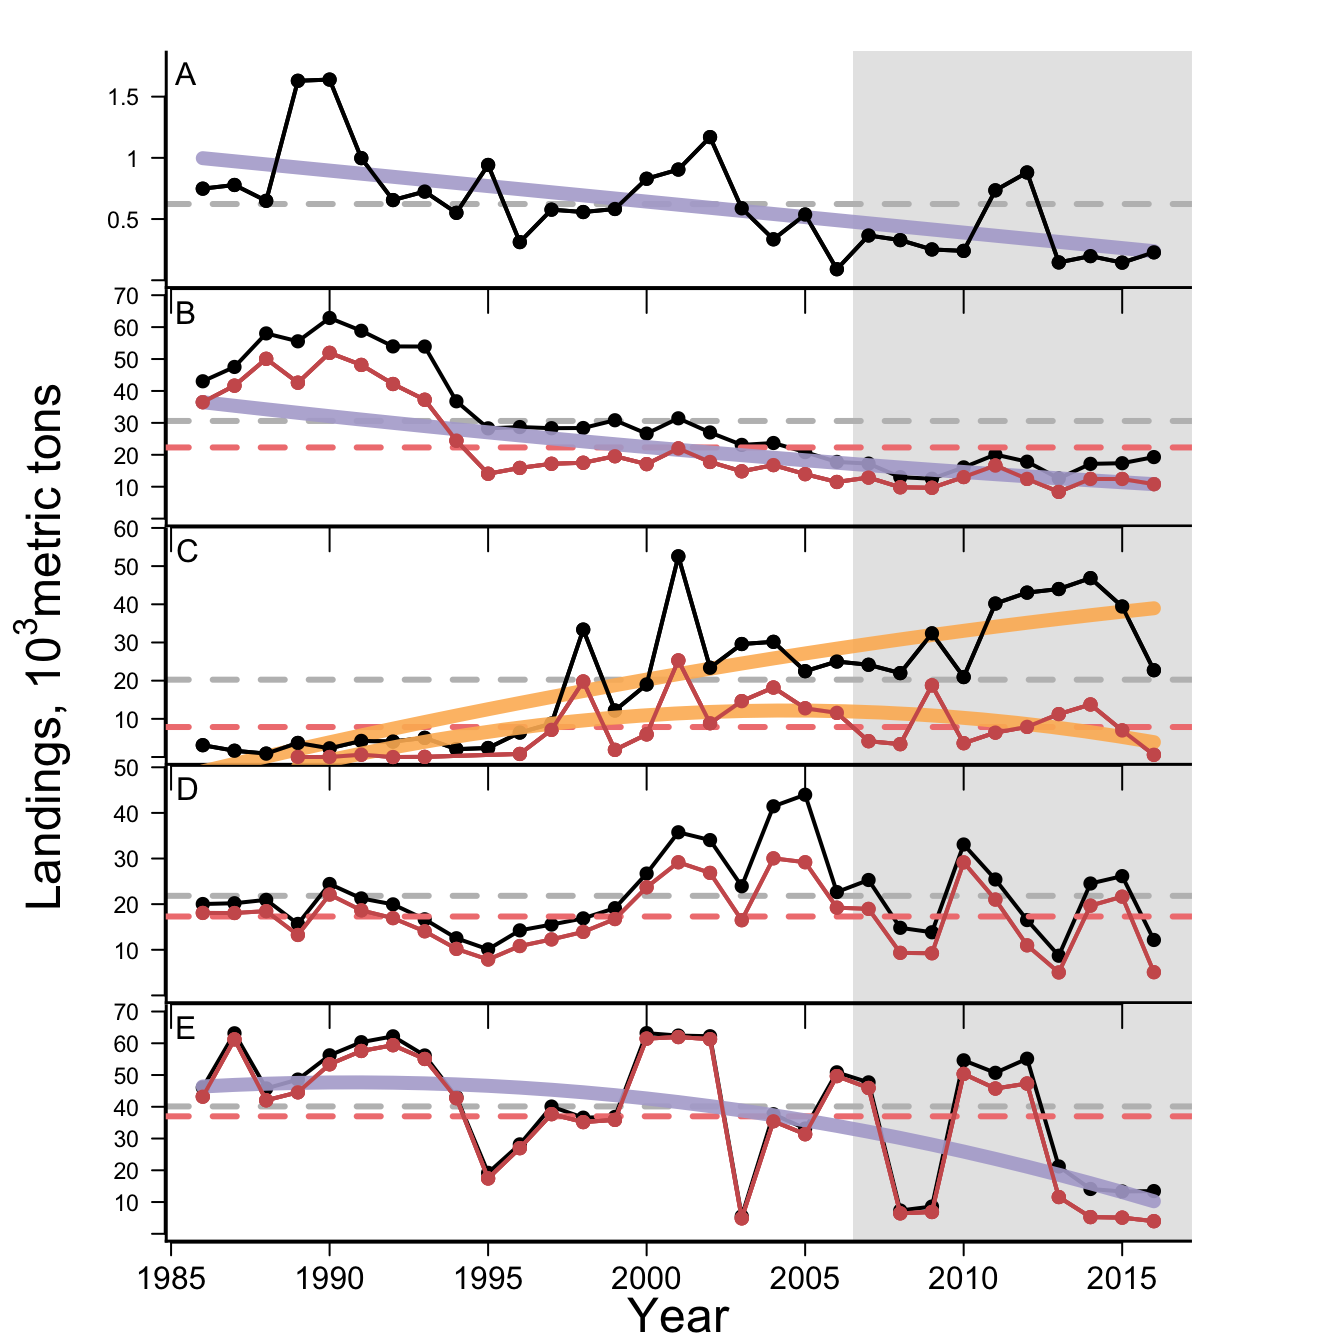
\includegraphics{landings_data_files/figure-latex/seafood-landings-1} 

}

\caption{NEFMC seafood specific landings (red) and total commericial landings (black) in Georges Bank (A: Apex predators, B: Piscivore, C: Planktivore, D: Benthivore, E: Benthos).}\label{fig:seafood-landings}
\end{figure}


\end{document}
